\documentclass{beamer}
\usepackage{tikz}
\usetikzlibrary{decorations.pathmorphing, shapes.misc, calc}
\usepackage{pgfplots}
\usepackage{pgfpages}
\usepackage{xcolor}
\usepackage{bm}


\usefonttheme{professionalfonts}%requiredformathspec
\usepackage[charter]{mathdesign}

% ubuntu fix for fira font...
% \usepackage{amsmath}
% \usepackage[no-math]{fontspec}
% \usepackage[charter]{mathdesign}
% \usefonttheme{professionalfonts} %required for mathspec
% \setsansfont[
%     Extension      = .otf,
%     UprightFont    = *-Light,
%     ItalicFont     = *-LightItalic,
%     BoldFont       = *-Regular,
%     BoldItalicFont = *-RegularItalic
% ]{FiraSans}
% \setmonofont[
%     Extension   = .otf,
%     UprightFont = *-Regular,
%     BoldFont    = *-Medium
% ]{FiraMono}

\setbeamercolor{background canvas}{bg=white}

\usetheme[
  sectionpage=progressbar,
  numbering=fraction,
  block=fill,
  progressbar=foot
]{metropolis}           % Use metropolis theme


%%% Section page template with picture

\makeatletter
\defbeamertemplate*{section page}{mytheme}[1][]{
  \centering
  \begin{minipage}{22em}
    \raggedright
    \usebeamercolor[fg]{section title}
    \usebeamerfont{section title}
    \insertsectionhead\\[-1ex]
    \usebeamertemplate*{progress bar in section page}
    \par
    \ifx\insertsubsectionhead\@empty\else%
      \usebeamercolor[fg]{subsection title}%
      \usebeamerfont{subsection title}%
      \insertsubsectionhead
    \fi
    \vskip0.5cm
    \ifstrempty{#1}{}{%
        #1%
    }
  \end{minipage}
  \par
  \vspace{\baselineskip}
}
\makeatother

%%% Define a command to include picture in section,
%%% make section, and revert to old template

\newcommand{\sectionpic}[2]{
   \setbeamertemplate{section page}[mytheme][#2]
   \section{#1}
   \setbeamertemplate{section page}[mytheme]
}

\definecolor{fc}{HTML}{1E90FF}
\definecolor{h}{HTML}{228B22}
\definecolor{bias}{HTML}{87CEFA}
\definecolor{noise}{HTML}{8B008B}
\definecolor{conv}{HTML}{FFA500}
\definecolor{pool}{HTML}{B22222}
\definecolor{up}{HTML}{B22222}
\definecolor{view}{HTML}{FFFFFF}
\definecolor{bn}{HTML}{FFD700}
\tikzset{fc/.style={black,draw=black,fill=fc,rectangle,minimum height=1cm}}
\tikzset{h/.style={black,draw=black,fill=h,rectangle,minimum height=1cm}}
\tikzset{bias/.style={black,draw=black,fill=bias,rectangle,minimum height=1cm}}
\tikzset{noise/.style={black,draw=black,fill=noise,rectangle,minimum height=1cm}}
\tikzset{conv/.style={black,draw=black,fill=conv,rectangle,minimum height=1cm}}
\tikzset{pool/.style={black,draw=black,fill=pool,rectangle,minimum height=1cm}}
\tikzset{up/.style={black,draw=black,fill=up,rectangle,minimum height=1cm}}
\tikzset{view/.style={black,draw=black,fill=view,rectangle,minimum height=1cm}}
\tikzset{bn/.style={black,draw=black,fill=bn,rectangle,minimum height=1cm}}


%% enable \pause in \align environments
\makeatletter
\let\save@measuring@true\measuring@true
\def\measuring@true{%
  \save@measuring@true
  \def\beamer@sortzero##1{\beamer@ifnextcharospec{\beamer@sortzeroread{##1}}{}}%
  \def\beamer@sortzeroread##1<##2>{}%
  \def\beamer@finalnospec{}%
}
\makeatother

% some equation stuff
\newcommand{\half}{\frac{1}{2}}
\renewcommand{\x}{\bm{x}}
\newcommand{\xh}{\hat{\bm{x}}}
\newcommand{\e}{\bm{e}}
\newcommand{\z}{\bm{z}}
\newcommand{\mz}{\bm{\mu}_{z}}
\newcommand{\w}{\bm{w}}
\newcommand{\bo}{\bm{b}}
\newcommand{\A}{\bm{A}}

\newcommand{\se}{\sigma_e}
\newcommand{\sz}{\bm{\sigma_z}}
\newcommand{\laz}{\bm{\lambda}_z}

\newcommand{\X}{\bm{X}}
\newcommand{\Z}{\bm{Z}}
\newcommand{\N}{\mathcal{N}}
\newcommand{\E}[2]{\text{E}_{#1}\left[#2\right]}
\newcommand{\KL}{\text{KL}}


\title{Rodent - Relevant ODE identifier}
\date{\today}
\author{
  Niklas Heim, Tom\'a\v s Pevn\'y , V\'aclav \v Sm\'idl\\
}
\institute{Artificial Intelligence Center}

\begin{document}

\maketitle

\begin{frame}{Rodent}
  \centering
  \begin{figure}
    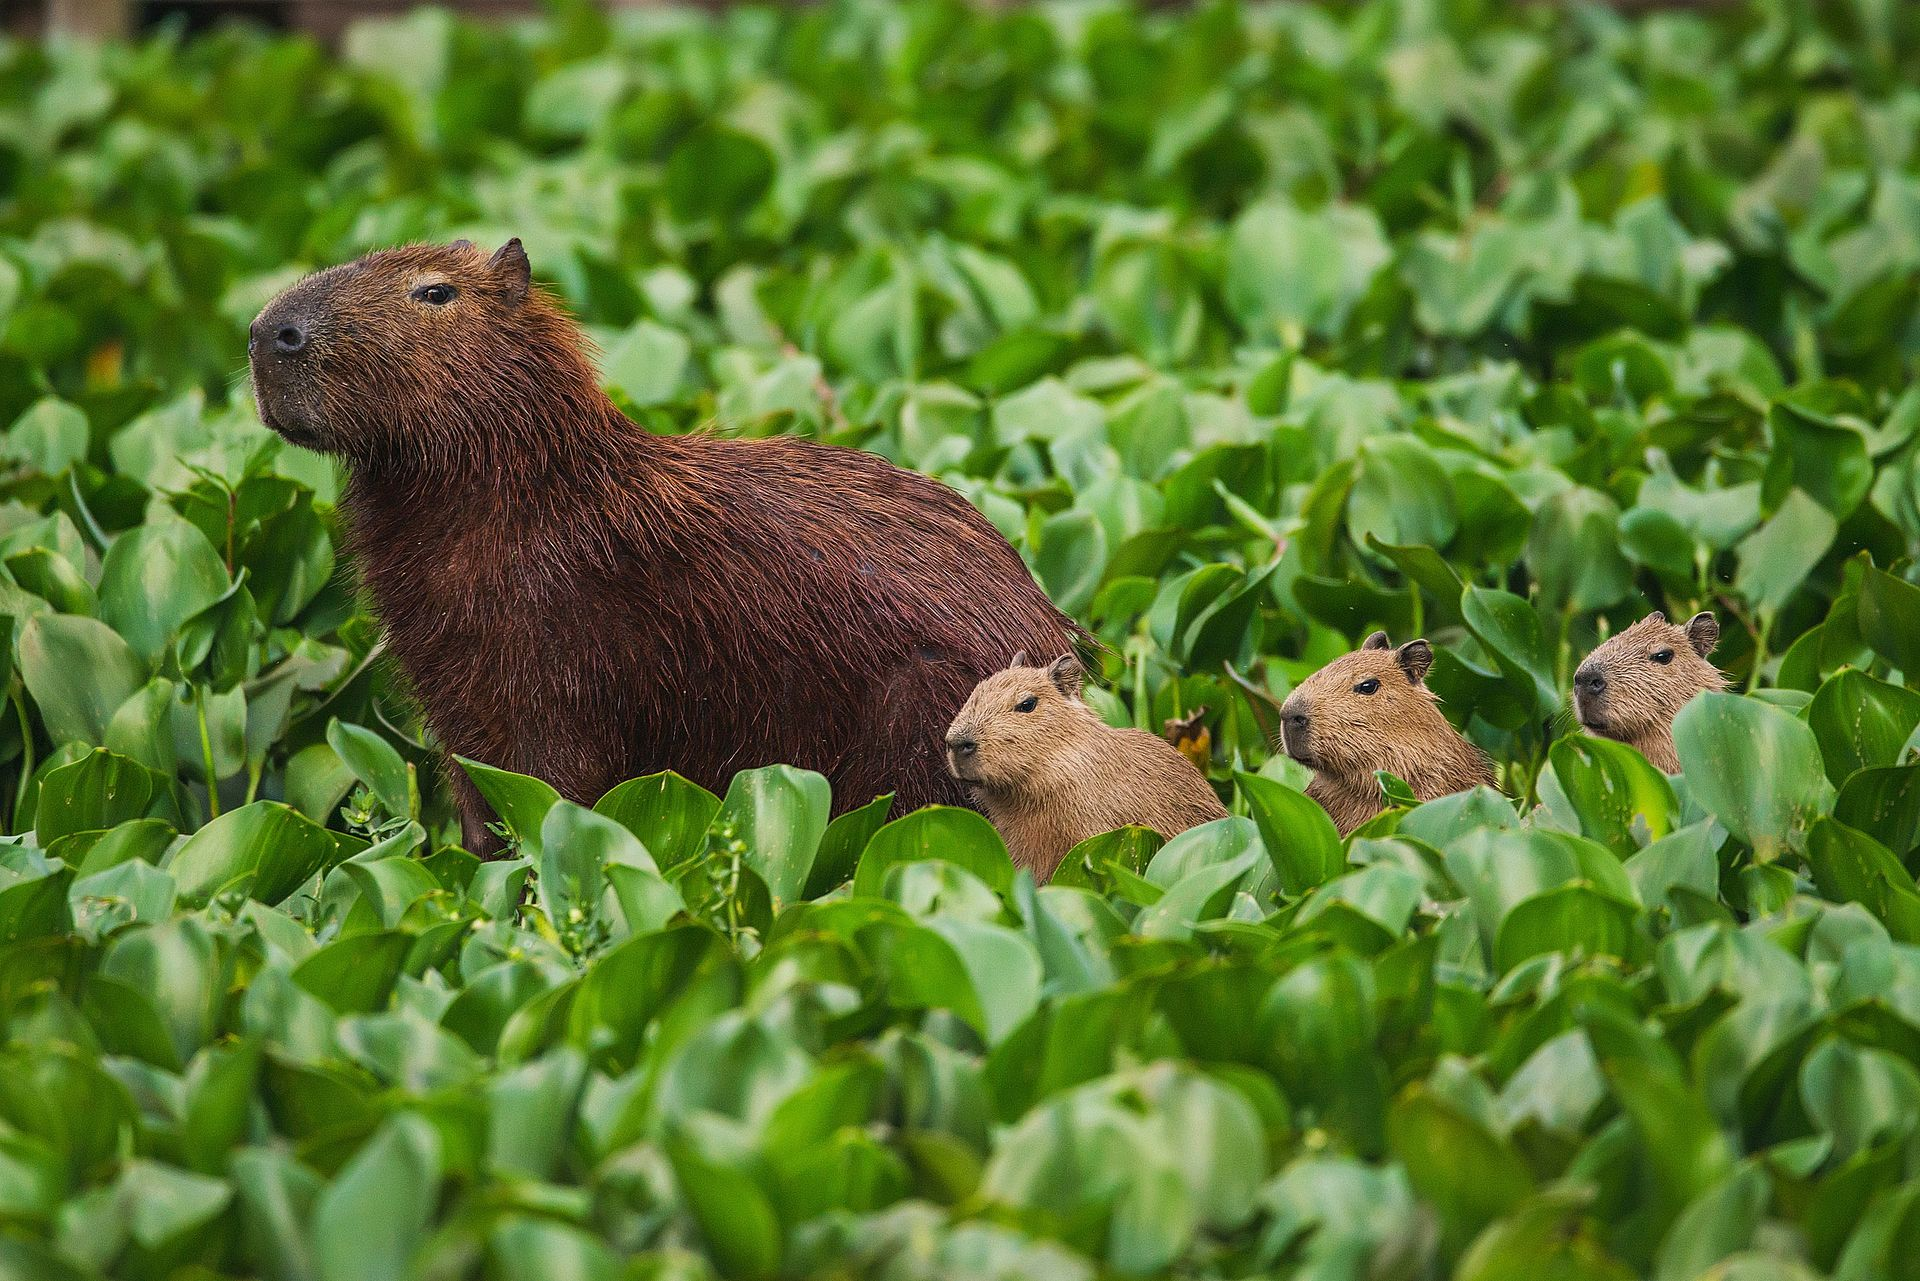
\includegraphics[width=0.8\linewidth]{figs/rodent.jpg}
  \end{figure}
  \color{black}
  \textbf{Rodent}: \textbf{R}elevant \textbf{o}rdinary differential equation
  i\textbf{dent}ifier
\end{frame}
\note{
  Today we will talk about rodents, which are a very investigative species,
  just like the framework we propose for model identification.\\

  Also, they are very agile on land and feel equally at home in the water, so
  they are in many ways very similar to ODEs and their generality.
}

\begin{frame}{Chirping fusion plasmas}
  \begin{figure}
    \centering
    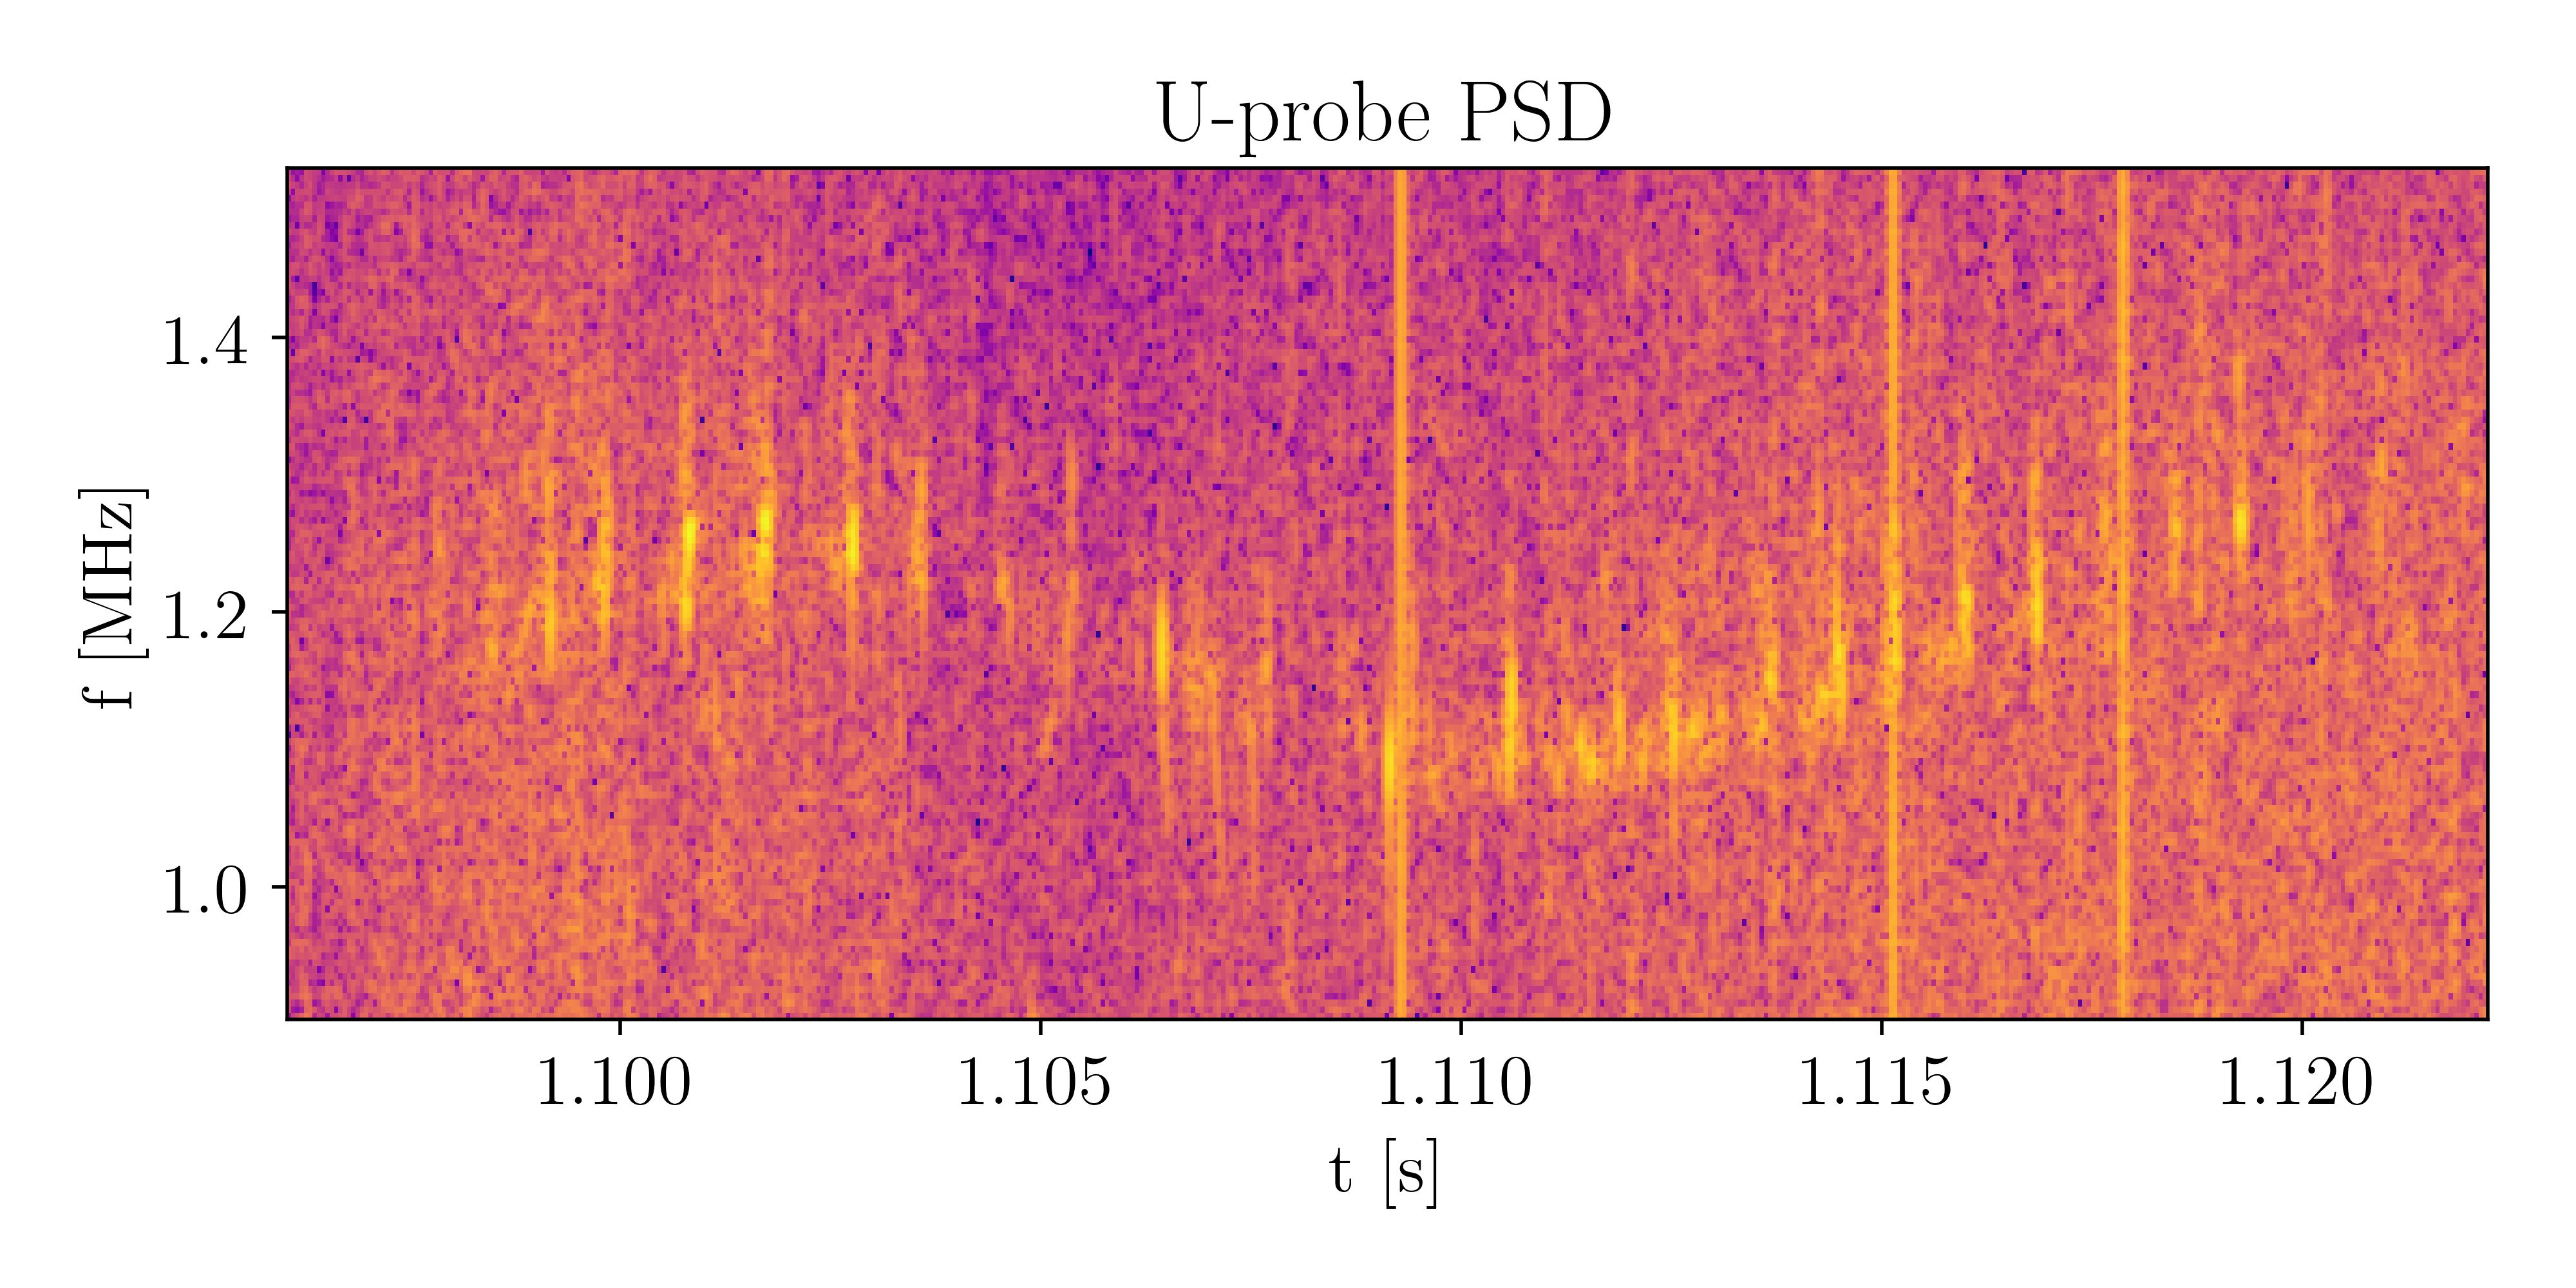
\includegraphics[width=.8\linewidth]{figs/alfven_patch_psd.png}
  \end{figure}
  \begin{itemize}
    \item scalar time-series that rarely contains \alert{Alfven modes}
    \item Alfvens are poorly understood
  \end{itemize}
\end{frame} 
\note{
  \begin{itemize}
    \item Alfven modes in Tokamaks
    \item poorly understood, anomalous frequencies, in the plasma
    \item typical problem of physicists: loads of data, few labels
    \item Physicists are interested in finding more alfvens in their data,
      but even better would be an \alert{interpretable/explainable} model
  \end{itemize}
}

\begin{frame}{Chirping fusion plasmas}
  \centering
  \resizebox{!}{.4\textwidth}{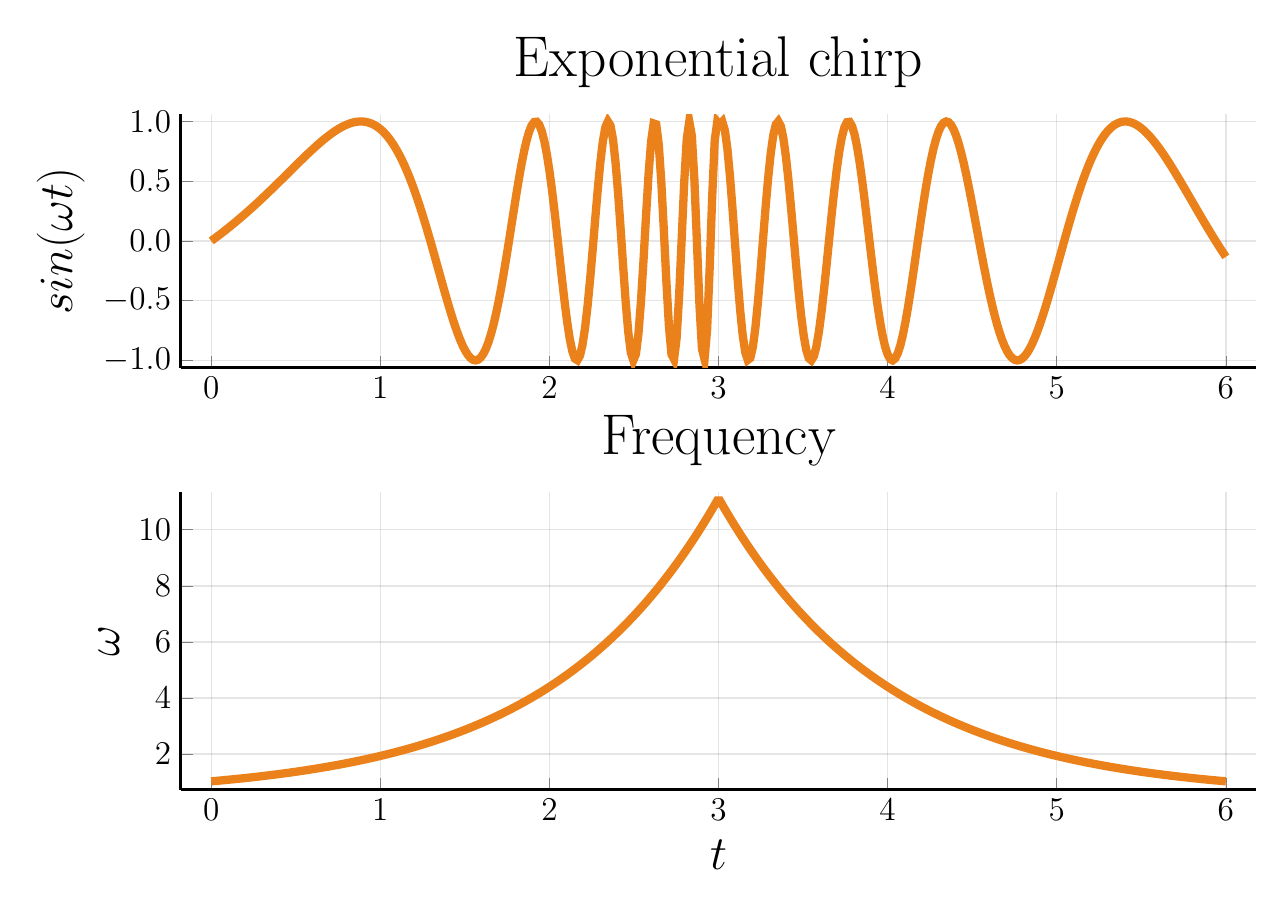
\begin{tikzpicture}[]
\begin{axis}[height = {47.977777777777774mm}, ylabel = {$\text{sin}(\omega t)$}, title = {Exponential chirp}, xmin = {-0.18}, xmax = {6.18}, ymax = {1.0599784777093217}, xlabel = {}, unbounded coords=jump,scaled x ticks = false,xlabel style = {font = {\fontsize{16 pt}{20.8 pt}\selectfont}, color = {rgb,1:red,0.00000000;green,0.00000000;blue,0.00000000}, draw opacity = 1.0, rotate = 0.0},xmajorgrids = true,xtick = {0.0,1.0,2.0,3.0,4.0,5.0,6.0},xticklabels = {$0$,$1$,$2$,$3$,$4$,$5$,$6$},xtick align = inside,xticklabel style = {font = {\fontsize{12 pt}{15.600000000000001 pt}\selectfont}, color = {rgb,1:red,0.00000000;green,0.00000000;blue,0.00000000}, draw opacity = 1.0, rotate = 0.0},x grid style = {color = {rgb,1:red,0.00000000;green,0.00000000;blue,0.00000000},
draw opacity = 0.1,
line width = 0.5,
solid},axis x line* = left,x axis line style = {color = {rgb,1:red,0.00000000;green,0.00000000;blue,0.00000000},
draw opacity = 1.0,
line width = 1,
solid},scaled y ticks = false,ylabel style = {font = {\fontsize{16 pt}{20.8 pt}\selectfont}, color = {rgb,1:red,0.00000000;green,0.00000000;blue,0.00000000}, draw opacity = 1.0, rotate = 0.0},ymajorgrids = true,ytick = {-1.0,-0.5,0.0,0.5,1.0},yticklabels = {$-1.0$,$-0.5$,$0.0$,$0.5$,$1.0$},ytick align = inside,yticklabel style = {font = {\fontsize{12 pt}{15.600000000000001 pt}\selectfont}, color = {rgb,1:red,0.00000000;green,0.00000000;blue,0.00000000}, draw opacity = 1.0, rotate = 0.0},y grid style = {color = {rgb,1:red,0.00000000;green,0.00000000;blue,0.00000000},
draw opacity = 0.1,
line width = 0.5,
solid},axis y line* = left,y axis line style = {color = {rgb,1:red,0.00000000;green,0.00000000;blue,0.00000000},
draw opacity = 1.0,
line width = 1,
solid},    xshift = 0.0mm,
    yshift = 53.62mm,
    axis background/.style={fill={rgb,1:red,1.00000000;green,1.00000000;blue,1.00000000}}
,title style = {font = {\fontsize{21 pt}{27.3 pt}\selectfont}, color = {rgb,1:red,0.00000000;green,0.00000000;blue,0.00000000}, draw opacity = 1.0, rotate = 0.0},legend style = {color = {rgb,1:red,0.00000000;green,0.00000000;blue,0.00000000},
draw opacity = 1.0,
line width = 1,
solid,fill = {rgb,1:red,1.00000000;green,1.00000000;blue,1.00000000},font = {\fontsize{12 pt}{15.600000000000001 pt}\selectfont}},colorbar style={title=}, ymin = {-1.0599945967550304}, width = {152.4mm}]\addplot+ [color = {rgb,1:red,0.92156863;green,0.50588235;blue,0.10588235},
draw opacity = 1.0,
line width = 3,
solid,mark = none,
mark size = 2.0,
mark options = {
    color = {rgb,1:red,0.00000000;green,0.00000000;blue,0.00000000}, draw opacity = 1.0,
    fill = {rgb,1:red,0.92156863;green,0.50588235;blue,0.10588235}, fill opacity = 1.0,
    line width = 1,
    rotate = 0,
    solid
},forget plot]coordinates {
(0.0, 0.0)
(0.015037593984962405, 0.015532826934182514)
(0.03007518796992481, 0.03130526617823803)
(0.045112781954887216, 0.047318661897177074)
(0.06015037593984962, 0.06357407772146233)
(0.07518796992481203, 0.08007226964905839)
(0.09022556390977443, 0.09681365715301653)
(0.10526315789473684, 0.11379829240290266)
(0.12030075187969924, 0.13102582750608235)
(0.13533834586466165, 0.1484954796728512)
(0.15037593984962405, 0.16620599420770338)
(0.16541353383458646, 0.18415560522773072)
(0.18045112781954886, 0.2023419940083206)
(0.19548872180451127, 0.2207622448560536)
(0.21052631578947367, 0.23941279840909224)
(0.22556390977443608, 0.2582894022665019)
(0.24060150375939848, 0.2773870588499827)
(0.2556390977443609, 0.2966999704045399)
(0.2706766917293233, 0.3162214810488342)
(0.2857142857142857, 0.33594401579149585)
(0.3007518796992481, 0.3558590164367359)
(0.3157894736842105, 0.37595687431134317)
(0.3308270676691729, 0.3962268597558394)
(0.3458646616541353, 0.4166570483354127)
(0.3609022556390977, 0.43723424374152886)
(0.37593984962406013, 0.4579438973731105)
(0.39097744360902253, 0.4787700246071993)
(0.40601503759398494, 0.49969511779340026)
(0.42105263157894735, 0.5207000560345325)
(0.43609022556390975, 0.5417640118481573)
(0.45112781954887216, 0.5628643548404639)
(0.46616541353383456, 0.5839765525658058)
(0.48120300751879697, 0.6050740687924953)
(0.49624060150375937, 0.6261282594487936)
(0.5112781954887218, 0.6471082665829252)
(0.5263157894736842, 0.667980910737974)
(0.5413533834586466, 0.6887105822172939)
(0.556390977443609, 0.7092591317992085)
(0.5714285714285714, 0.7295857615519312)
(0.5864661654135338, 0.749646916501473)
(0.6015037593984962, 0.7693961780174857)
(0.6165413533834586, 0.7887841599051835)
(0.631578947368421, 0.8077584083263425)
(0.6466165413533834, 0.826263306819547)
(0.6616541353383458, 0.8442399878498895)
(0.6766917293233082, 0.8616262524918057)
(0.6917293233082706, 0.8783565000360443)
(0.706766917293233, 0.8943616695132987)
(0.7218045112781954, 0.9095691953429426)
(0.7368421052631579, 0.9239029795456272)
(0.7518796992481203, 0.9372833832030251)
(0.7669172932330827, 0.949627240106241)
(0.7819548872180451, 0.9608478958055848)
(0.7969924812030075, 0.970855275557292)
(0.8120300751879699, 0.9795559849557516)
(0.8270676691729323, 0.9868534473406548)
(0.8421052631578947, 0.9926480823743746)
(0.8571428571428571, 0.9968375304922752)
(0.8721804511278195, 0.9993169282331045)
(0.8872180451127819, 0.9999792397527835)
(0.9022556390977443, 0.9987156501062855)
(0.9172932330827067, 0.9954160261411861)
(0.9323308270676691, 0.9899694510737646)
(0.9473684210526315, 0.982264839003581)
(0.9624060150375939, 0.97219163575289)
(0.9774436090225563, 0.9596406124788228)
(0.9924812030075187, 0.9445047584826931)
(1.0075187969924813, 0.9266802795135551)
(1.0225563909774436, 0.9060677076114131)
(1.037593984962406, 0.8825731281359228)
(1.0526315789473684, 0.8561095290531223)
(1.0676691729323309, 0.8265982767771378)
(1.0827067669172932, 0.7939707218547606)
(1.0977443609022557, 0.7581699365045353)
(1.112781954887218, 0.7191525844424433)
(1.1278195488721805, 0.6768909215051653)
(1.1428571428571428, 0.6313749232794169)
(1.1578947368421053, 0.5826145332210013)
(1.1729323308270676, 0.5306420215589108)
(1.1879699248120301, 0.4755144415876872)
(1.2030075187969924, 0.417316165717291)
(1.218045112781955, 0.3561614788397306)
(1.2330827067669172, 0.292197201157696)
(1.2481203007518797, 0.2256053065827704)
(1.263157894736842, 0.1566054961418234)
(1.2781954887218046, 0.08545767853705642)
(1.2932330827067668, 0.012464302114806355)
(1.3082706766917294, -0.062027525938608934)
(1.3233082706766917, -0.13762420625849595)
(1.3383458646616542, -0.21388418215813657)
(1.3533834586466165, -0.29031693446173673)
(1.368421052631579, -0.3663825375247599)
(1.3834586466165413, -0.44149188680142315)
(1.3984962406015038, -0.5150077168594409)
(1.413533834586466, -0.5862465362728423)
(1.4285714285714286, -0.6544816118646459)
(1.443609022556391, -0.7189471387565369)
(1.4586466165413534, -0.7788437339563152)
(1.4736842105263157, -0.8333453890266109)
(1.4887218045112782, -0.8816080108891875)
(1.5037593984962405, -0.9227796680995308)
(1.518796992481203, -0.956012641971665)
(1.5338345864661653, -0.9804773566795417)
(1.5488721804511278, -0.9953782288128883)
(1.5639097744360901, -0.9999714337308522)
(1.5789473684210527, -0.993584532398999)
(1.593984962406015, -0.9756378372952637)
(1.6090225563909775, -0.9456673187076763)
(1.6240601503759398, -0.9033487628966544)
(1.6390977443609023, -0.8485227911461123)
(1.6541353383458646, -0.7812202342185036)
(1.669172932330827, -0.7016872314008702)
(1.6842105263157894, -0.6104092892981984)
(1.699248120300752, -0.5081333959701588)
(1.7142857142857142, -0.3958871453357203)
(1.7293233082706767, -0.27499369083269687)
(1.744360902255639, -0.14708122355307338)
(1.7593984962406015, -0.01408556763524969)
(1.7744360902255638, 0.12175558447802236)
(1.7894736842105263, 0.25791829950811074)
(1.8045112781954886, 0.3916193620321292)
(1.8195488721804511, 0.5198559238626532)
(1.8345864661654134, 0.6394590031626903)
(1.849624060150376, 0.7471616840348845)
(1.8646616541353382, 0.839682435609116)
(1.8796992481203008, 0.9138234013740115)
(1.894736842105263, 0.9665827955800265)
(1.9097744360902256, 0.9952796810728297)
(1.9248120300751879, 0.9976883975645149)
(1.9398496240601504, 0.9721787780547089)
(1.9548872180451127, 0.9178570649247716)
(1.9699248120300752, 0.8347011641223049)
(1.9849624060150375, 0.7236826232502497)
(2.0, 0.5868665760062134)
(2.0150375939849625, 0.4274799720900777)
(2.030075187969925, 0.24993784040852512)
(2.045112781954887, 0.0598172641813605)
(2.0601503759398496, -0.13623065865015058)
(2.075187969924812, -0.3306391733325086)
(2.0902255639097747, -0.5151604444874551)
(2.1052631578947367, -0.6811787438005676)
(2.1203007518796992, -0.8200999632635048)
(2.1353383458646618, -0.9238093270588845)
(2.1503759398496243, -0.9851822927189389)
(2.1654135338345863, -0.9986259683357568)
(2.180451127819549, -0.960620354520633)
(2.1954887218045114, -0.8702209615014255)
(2.210526315789474, -0.7294776604445877)
(2.225563909774436, -0.5437199903914526)
(2.2406015037593985, -0.32165768244256954)
(2.255639097744361, -0.07524806646969605)
(2.2706766917293235, 0.18070957805701907)
(2.2857142857142856, 0.4292778640622669)
(2.300751879699248, 0.6523867672179474)
(2.3157894736842106, 0.8321157128420925)
(2.330827067669173, 0.9521931173271634)
(2.345864661654135, 0.9996165186857917)
(2.3609022556390977, 0.9662585798294699)
(2.3759398496240602, 0.8502909361192742)
(2.3909774436090228, 0.6572348897771381)
(2.406015037593985, 0.40044183621943436)
(2.4210526315789473, 0.10082354046157166)
(2.43609022556391, -0.21430157513492132)
(2.4511278195488724, -0.5133020121132731)
(2.4661654135338344, -0.7632133927133492)
(2.481203007518797, -0.9334177626719975)
(2.4962406015037595, -0.9996876247340242)
(2.511278195488722, -0.9481202593210727)
(2.526315789473684, -0.7783802034843558)
(2.5413533834586466, -0.5056219346202308)
(2.556390977443609, -0.16051007408165835)
(2.5714285714285716, 0.2130862124035105)
(2.5864661654135337, 0.5628651094024236)
(2.601503759398496, 0.8350765392001415)
(2.6165413533834587, 0.9829993114362737)
(2.6315789473684212, 0.975724254567175)
(2.6466165413533833, 0.8056863182407257)
(2.661654135338346, 0.49322897820786576)
(2.6766917293233083, 0.08664365412408687)
(2.691729323308271, -0.34332116073400437)
(2.706766917293233, -0.7145371158448738)
(2.7218045112781954, -0.9489642509756696)
(2.736842105263158, -0.9899731184656595)
(2.7518796992481205, -0.8178698259059823)
(2.7669172932330826, -0.45946596191795297)
(2.781954887218045, 0.012013762694011696)
(2.7969924812030076, 0.4887810389760934)
(2.81203007518797, 0.851484786571285)
(2.827067669172932, 0.9994133990758663)
(2.8421052631578947, 0.880789640511838)
(2.857142857142857, 0.5141654072065032)
(2.8721804511278197, -0.007611700498730116)
(2.887218045112782, -0.5359200347134692)
(2.9022556390977443, -0.9061586238764959)
(2.917293233082707, -0.9898568639373141)
(2.9323308270676693, -0.7433683941003963)
(2.9473684210526314, -0.23461357116844359)
(2.962406015037594, 0.3669899626645943)
(2.9774436090225564, 0.8414121801457386)
(2.992481203007519, 0.9978912708404066)
(3.007518796992481, 0.973428267169813)
(3.0225563909774436, 0.9968211438661343)
(3.037593984962406, 0.9256186532147884)
(3.0526315789473686, 0.7686438944112862)
(3.0676691729323307, 0.5423170123435654)
(3.082706766917293, 0.2687418959530862)
(3.0977443609022557, -0.0265985987018163)
(3.112781954887218, -0.3172951928720133)
(3.1278195488721803, -0.5783785428695778)
(3.142857142857143, -0.788395867783239)
(3.1578947368421053, -0.9310399965721582)
(3.172932330827068, -0.9962278573373212)
(3.18796992481203, -0.9805833511037563)
(3.2030075187969924, -0.887334937385833)
(3.218045112781955, -0.7256865224124585)
(3.2330827067669174, -0.5097580659466348)
(3.2481203007518795, -0.25721777371352844)
(3.263157894736842, 0.012259767849738593)
(3.2781954887218046, 0.2785750202944956)
(3.293233082706767, 0.522700634640275)
(3.308270676691729, 0.727989628495187)
(3.3233082706766917, 0.881214989493283)
(3.338345864661654, 0.97328931762714)
(3.3533834586466167, 0.9996418930642754)
(3.3684210526315788, 0.9602576092252377)
(3.3834586466165413, 0.8594057310665701)
(3.398496240601504, 0.7051051460568958)
(3.4135338345864663, 0.5083859399763372)
(3.4285714285714284, 0.28241454045986575)
(3.443609022556391, 0.04155157069191223)
(3.4586466165413534, -0.19959145005504358)
(3.473684210526316, -0.42703746614550664)
(3.488721804511278, -0.628222271253056)
(3.5037593984962405, -0.792628878061333)
(3.518796992481203, -0.9122537036146814)
(3.5338345864661656, -0.9818932012884349)
(3.5488721804511276, -0.9992514877324773)
(3.56390977443609, -0.9648799194313006)
(3.5789473684210527, -0.8819680314824266)
(3.593984962406015, -0.7560115132193609)
(3.6090225563909772, -0.5943868886887679)
(3.6240601503759398, -0.4058643730465767)
(3.6390977443609023, -0.20009018831928807)
(3.654135338345865, 0.012932267701030212)
(3.669172932330827, 0.22333625223568615)
(3.6842105263157894, 0.4218385928449833)
(3.699248120300752, 0.6001226186582591)
(3.7142857142857144, 0.7511451509226682)
(3.7293233082706765, 0.8693606639293622)
(3.744360902255639, 0.9508604908504611)
(3.7593984962406015, 0.9934292051608885)
(3.774436090225564, 0.9965239124747339)
(3.789473684210526, 0.9611850518633793)
(3.8045112781954886, 0.8898893941220399)
(3.819548872180451, 0.786357246319125)
(3.8345864661654137, 0.655326473755281)
(3.8496240601503757, 0.5023059071196672)
(3.8646616541353382, 0.333320108947774)
(3.8796992481203008, 0.15465643594078543)
(3.8947368421052633, -0.02737603681463521)
(3.9097744360902253, -0.20666775811386157)
(3.924812030075188, -0.37750385384492463)
(3.9398496240601504, -0.5347286816058793)
(3.954887218045113, -0.6738769745508376)
(3.969924812030075, -0.7912703469571135)
(3.9849624060150375, -0.8840793569855778)
(4.0, -0.9503525490905652)
(4.015037593984962, -0.9890149089596318)
(4.030075187969925, -0.999838949470701)
(4.045112781954887, -0.9833922092578732)
(4.06015037593985, -0.9409652970638644)
(4.075187969924812, -0.8744847728360857)
(4.090225563909774, -0.7864151430430624)
(4.105263157894737, -0.6796540885759792)
(4.120300751879699, -0.5574247659956576)
(4.135338345864661, -0.42316865408915166)
(4.150375939849624, -0.28044198406583487)
(4.165413533834586, -0.13281831778838596)
(4.180451127819549, 0.016200653715995546)
(4.195488721804511, 0.1632645103713014)
(4.2105263157894735, 0.30524259474879145)
(4.225563909774436, 0.43928093229649945)
(4.2406015037593985, 0.5628473211671823)
(4.2556390977443606, 0.6737646900169978)
(4.2706766917293235, 0.7702331284023703)
(4.285714285714286, 0.8508412477190186)
(4.3007518796992485, 0.9145677311412197)
(4.315789473684211, 0.9607740805385716)
(4.330827067669173, 0.9891896700024728)
(4.345864661654136, 0.9998902735297539)
(4.360902255639098, 0.9932712533965303)
(4.37593984962406, 0.9700165810352858)
(4.390977443609023, 0.9310648192005695)
(4.406015037593985, 0.8775731282454001)
(4.421052631578948, 0.8108802756138016)
(4.43609022556391, 0.7324695310496274)
(4.451127819548872, 0.6439322249818736)
(4.466165413533835, 0.5469326380502957)
(4.481203007518797, 0.44317477924943227)
(4.496240601503759, 0.33437150163385104)
(4.511278195488722, 0.2222163003615532)
(4.526315789473684, 0.10835803997265916)
(4.541353383458647, -0.005621232347021047)
(4.556390977443609, -0.11822531216719173)
(4.571428571428571, -0.2280596985496731)
(4.586466165413534, -0.3338443491398682)
(4.601503759398496, -0.43442344130329763)
(4.616541353383458, -0.5287722942231361)
(4.631578947368421, -0.6160016410799706)
(4.646616541353383, -0.6953594661937494)
(4.661654135338346, -0.7662306400023337)
(4.676691729323308, -0.8281345957366776)
(4.69172932330827, -0.8807212964267205)
(4.706766917293233, -0.923765740247333)
(4.7218045112781954, -0.957161246995341)
(4.7368421052631575, -0.9809117594568726)
(4.7518796992481205, -0.9951233813197677)
(4.7669172932330826, -0.9999953587984921)
(4.7819548872180455, -0.9958106969016352)
(4.796992481203008, -0.9829265838543432)
(4.81203007518797, -0.9617647790947956)
(4.827067669172933, -0.9328021019345961)
(4.842105263157895, -0.8965611397830378)
(4.857142857142857, -0.853601277098296)
(4.87218045112782, -0.80451012920035)
(4.887218045112782, -0.749895448962599)
(4.902255639097745, -0.6903775593443785)
(4.917293233082707, -0.6265823508433268)
(4.932330827067669, -0.5591348703044314)
(4.947368421052632, -0.4886535161568236)
(4.962406015037594, -0.4157448450667665)
(4.977443609022556, -0.3409989861776801)
(4.992481203007519, -0.2649856515173895)
(5.007518796992481, -0.18825072473570106)
(5.022556390977444, -0.11131340502512047)
(5.037593984962406, -0.03466387879928122)
(5.052631578947368, 0.041238511623961596)
(5.067669172932331, 0.11596663554987802)
(5.082706766917293, 0.18912651254233262)
(5.097744360902255, 0.26035785805447637)
(5.112781954887218, 0.32933427232205026)
(5.12781954887218, 0.3957631086389847)
(5.142857142857143, 0.4593850565367375)
(5.157894736842105, 0.5199734744122114)
(5.172932330827067, 0.577333504862032)
(5.18796992481203, 0.6313010044449311)
(5.203007518796992, 0.6817413178657785)
(5.2180451127819545, 0.7285479247048048)
(5.2330827067669174, 0.7716409848492226)
(5.2481203007518795, 0.8109658067613341)
(5.2631578947368425, 0.8464912606720285)
(5.2781954887218046, 0.8782081567510531)
(5.293233082706767, 0.9061276063006024)
(5.30827067669173, 0.9302793820676837)
(5.323308270676692, 0.9507102918902995)
(5.338345864661654, 0.9674825780962438)
(5.353383458646617, 0.9806723533717112)
(5.368421052631579, 0.9903680822173186)
(5.383458646616542, 0.9966691156167322)
(5.398496240601504, 0.9996842851606856)
(5.413533834586466, 0.9995305615978256)
(5.428571428571429, 0.9963317816229608)
(5.443609022556391, 0.9902174456610201)
(5.458646616541353, 0.9813215884583921)
(5.473684210526316, 0.9697817234484266)
(5.488721804511278, 0.9557378611102062)
(5.503759398496241, 0.9393316008841542)
(5.518796992481203, 0.9207052956391706)
(5.533834586466165, 0.9000012871981566)
(5.548872180451128, 0.8773612110160696)
(5.56390977443609, 0.8529253677613159)
(5.578947368421052, 0.8268321592714455)
(5.593984962406015, 0.7992175861320514)
(5.609022556390977, 0.770214803958095)
(5.62406015037594, 0.7399537353340361)
(5.639097744360902, 0.7085607342883233)
(5.654135338345864, 0.6761583001339674)
(5.669172932330827, 0.6428648374956816)
(5.684210526315789, 0.6087944593611432)
(5.6992481203007515, 0.5740568300354553)
(5.714285714285714, 0.5387570449400877)
(5.7293233082706765, 0.5029955442773281)
(5.7443609022556394, 0.4668680576753804)
(5.7593984962406015, 0.43046557703499155)
(5.774436090225564, 0.39387435491346967)
(5.7894736842105265, 0.357175925903798)
(5.804511278195489, 0.3204471485934218)
(5.819548872180451, 0.2837602658173166)
(5.834586466165414, 0.24718298105166026)
(5.849624060150376, 0.21077854892646988)
(5.864661654135339, 0.17460587796675744)
(5.879699248120301, 0.13871964380114893)
(5.894736842105263, 0.10317041120359485)
(5.909774436090226, 0.0680047634572169)
(5.924812030075188, 0.03326543764868806)
(5.93984962406015, -0.0010085353833143176)
(5.954887218045113, -0.03478168761178161)
(5.969924812030075, -0.06802196795803657)
(5.984962406015038, -0.10070059496208163)
(6.0, -0.1327919088525176)
};
\end{axis}
\begin{axis}[height = {53.62222222222222mm}, ylabel = {$\omega$}, title = {Frequency}, xmin = {-0.18}, xmax = {6.18}, ymax = {11.345504091213732}, xlabel = {$t$}, unbounded coords=jump,scaled x ticks = false,xlabel style = {font = {\fontsize{16 pt}{20.8 pt}\selectfont}, color = {rgb,1:red,0.00000000;green,0.00000000;blue,0.00000000}, draw opacity = 1.0, rotate = 0.0},xmajorgrids = true,xtick = {0.0,1.0,2.0,3.0,4.0,5.0,6.0},xticklabels = {$0$,$1$,$2$,$3$,$4$,$5$,$6$},xtick align = inside,xticklabel style = {font = {\fontsize{12 pt}{15.600000000000001 pt}\selectfont}, color = {rgb,1:red,0.00000000;green,0.00000000;blue,0.00000000}, draw opacity = 1.0, rotate = 0.0},x grid style = {color = {rgb,1:red,0.00000000;green,0.00000000;blue,0.00000000},
draw opacity = 0.1,
line width = 0.5,
solid},axis x line* = left,x axis line style = {color = {rgb,1:red,0.00000000;green,0.00000000;blue,0.00000000},
draw opacity = 1.0,
line width = 1,
solid},scaled y ticks = false,ylabel style = {font = {\fontsize{16 pt}{20.8 pt}\selectfont}, color = {rgb,1:red,0.00000000;green,0.00000000;blue,0.00000000}, draw opacity = 1.0, rotate = 0.0},ymajorgrids = true,ytick = {2.0,4.0,6.0,8.0,10.0},yticklabels = {$2$,$4$,$6$,$8$,$10$},ytick align = inside,yticklabel style = {font = {\fontsize{12 pt}{15.600000000000001 pt}\selectfont}, color = {rgb,1:red,0.00000000;green,0.00000000;blue,0.00000000}, draw opacity = 1.0, rotate = 0.0},y grid style = {color = {rgb,1:red,0.00000000;green,0.00000000;blue,0.00000000},
draw opacity = 0.1,
line width = 0.5,
solid},axis y line* = left,y axis line style = {color = {rgb,1:red,0.00000000;green,0.00000000;blue,0.00000000},
draw opacity = 1.0,
line width = 1,
solid},    xshift = 0.0mm,
    yshift = 0.0mm,
    axis background/.style={fill={rgb,1:red,1.00000000;green,1.00000000;blue,1.00000000}}
,title style = {font = {\fontsize{21 pt}{27.3 pt}\selectfont}, color = {rgb,1:red,0.00000000;green,0.00000000;blue,0.00000000}, draw opacity = 1.0, rotate = 0.0},legend style = {color = {rgb,1:red,0.00000000;green,0.00000000;blue,0.00000000},
draw opacity = 1.0,
line width = 1,
solid,fill = {rgb,1:red,1.00000000;green,1.00000000;blue,1.00000000},font = {\fontsize{12 pt}{15.600000000000001 pt}\selectfont}},colorbar style={title=}, ymin = {0.7244027934597941}, width = {152.4mm}]\addplot+ [color = {rgb,1:red,0.92156863;green,0.50588235;blue,0.10588235},
draw opacity = 1.0,
line width = 3,
solid,mark = none,
mark size = 2.0,
mark options = {
    color = {rgb,1:red,0.00000000;green,0.00000000;blue,0.00000000}, draw opacity = 1.0,
    fill = {rgb,1:red,0.92156863;green,0.50588235;blue,0.10588235}, fill opacity = 1.0,
    line width = 1,
    rotate = 0,
    solid
},forget plot]coordinates {
(0.0, 1.025)
(0.015037593984962405, 1.0329745313688474)
(0.03007518796992481, 1.0410701925482715)
(0.045112781954887216, 1.0492888234496516)
(0.06015037593984962, 1.0576322919318546)
(0.07518796992481203, 1.0661024942257458)
(0.09022556390977443, 1.0747013553651477)
(0.10526315789473684, 1.083430829624345)
(0.12030075187969924, 1.0922929009622346)
(0.13533834586466165, 1.101289583473223)
(0.15037593984962405, 1.1104229218449726)
(0.16541353383458646, 1.1196949918230987)
(0.18045112781954886, 1.1291079006829292)
(0.19548872180451127, 1.1386637877084258)
(0.21052631578947367, 1.1483648246783835)
(0.22556390977443608, 1.1582132163600123)
(0.24060150375939848, 1.1682112010100179)
(0.2556390977443609, 1.1783610508832933)
(0.2706766917293233, 1.1886650727493375)
(0.2857142857142857, 1.199125608416517)
(0.3007518796992481, 1.2097450352642922)
(0.3157894736842105, 1.220525766783528)
(0.3308270676691729, 1.2314702531250104)
(0.3458646616541353, 1.2425809816562945)
(0.3609022556390977, 1.253860477527014)
(0.37593984962406013, 1.2653113042427728)
(0.39097744360902253, 1.2769360642477587)
(0.40601503759398494, 1.2887373995162017)
(0.42105263157894735, 1.3007179921528214)
(0.43609022556390975, 1.3128805650023891)
(0.45112781954887216, 1.3252278822685568)
(0.46616541353383456, 1.337762750142077)
(0.48120300751879697, 1.3504880174385723)
(0.49624060150375937, 1.3634065762459873)
(0.5112781954887218, 1.3765213625818782)
(0.5263157894736842, 1.389835357060686)
(0.5413533834586466, 1.4033515855711431)
(0.556390977443609, 1.417073119963972)
(0.5714285714285714, 1.4310030787500283)
(0.5864661654135338, 1.4451446278090487)
(0.6015037593984962, 1.4595009811091646)
(0.6165413533834586, 1.4740754014373456)
(0.631578947368421, 1.4888712011409355)
(0.6466165413533834, 1.5038917428804561)
(0.6616541353383458, 1.5191404403938413)
(0.6766917293233082, 1.5346207592722827)
(0.6917293233082706, 1.550336217747859)
(0.706766917293233, 1.566290387493129)
(0.7218045112781954, 1.5824868944328712)
(0.7368421052631579, 1.5989294195681496)
(0.7518796992481203, 1.6156216998129032)
(0.7669172932330827, 1.6325675288432362)
(0.7819548872180451, 1.6497707579596141)
(0.7969924812030075, 1.6672352969621522)
(0.8120300751879699, 1.684965115039201)
(0.8270676691729323, 1.70296424166943)
(0.8421052631578947, 1.7212367675376103)
(0.8571428571428571, 1.7397868454643122)
(0.8721804511278195, 1.758618691349721)
(0.8872180451127819, 1.7777365851317894)
(0.9022556390977443, 1.7971448717589469)
(0.9172932330827067, 1.816847962177578)
(0.9323308270676691, 1.8368503343345075)
(0.9473684210526315, 1.857156534194707)
(0.9624060150375939, 1.8777711767744631)
(0.9774436090225563, 1.8986989471902382)
(0.9924812030075187, 1.9199446017234618)
(1.0075187969924813, 1.9415129689014987)
(1.0225563909774436, 1.963408950595033)
(1.037593984962406, 1.9856375231321228)
(1.0526315789473684, 2.008203738429178)
(1.0676691729323309, 2.0311127251391143)
(1.0827067669172932, 2.0543696898169497)
(1.0977443609022557, 2.077979918103104)
(1.112781954887218, 2.101948775924674)
(1.1278195488721805, 2.126281710714956)
(1.1428571428571428, 2.1509842526514884)
(1.1578947368421053, 2.176062015912903)
(1.1729323308270676, 2.201520699954867)
(1.1879699248120301, 2.2273660908054067)
(1.2030075187969924, 2.2536040623799036)
(1.218045112781955, 2.2802405778160697)
(1.2330827067669172, 2.307281690829192)
(1.2481203007518797, 2.334733547087975)
(1.263157894736842, 2.36260238561127)
(1.2781954887218046, 2.390894540186027)
(1.2932330827067668, 2.419616440806781)
(1.3082706766917294, 2.4487746151370073)
(1.3233082706766917, 2.4783756899926717)
(1.3383458646616542, 2.508426392848313)
(1.3533834586466165, 2.5389335533660087)
(1.368421052631579, 2.569904104947557)
(1.3834586466165413, 2.6013450863102436)
(1.3984962406015038, 2.6332636430865377)
(1.413533834586466, 2.6656670294480906)
(1.4285714285714286, 2.6985626097544007)
(1.443609022556391, 2.7319578602265175)
(1.4586466165413534, 2.7658603706461786)
(1.4736842105263157, 2.800277846080743)
(1.4887218045112782, 2.8352181086343347)
(1.5037593984962405, 2.8706890992255834)
(1.518796992481203, 2.9066988793923625)
(1.5338345864661653, 2.9432556331239517)
(1.5488721804511278, 2.9803676687210188)
(1.5639097744360901, 3.018043420683858)
(1.5789473684210527, 3.056291451629313)
(1.593984962406015, 3.0951204542368074)
(1.6090225563909775, 3.134539253223948)
(1.6240601503759398, 3.1745568073521278)
(1.6390977443609023, 3.2151822114625928)
(1.6541353383458646, 3.256424698543441)
(1.669172932330827, 3.2982936418280135)
(1.6842105263157894, 3.3407985569251637)
(1.699248120300752, 3.38394910398188)
(1.7142857142857142, 3.427755089878762)
(1.7293233082706767, 3.472226470458841)
(1.744360902255639, 3.5173733527902553)
(1.7593984962406015, 3.5632059974633035)
(1.7744360902255638, 3.6097348209223754)
(1.7894736842105263, 3.6569703978333146)
(1.8045112781954886, 3.704923463486733)
(1.8195488721804511, 3.7536049162378378)
(1.8345864661654134, 3.803025819983314)
(1.849624060150376, 3.8531974066758283)
(1.8646616541353382, 3.9041310788767323)
(1.8796992481203008, 3.955838412347534)
(1.894736842105263, 4.008331158680741)
(1.9097744360902256, 4.061621247970654)
(1.9248120300751879, 4.1157207915247405)
(1.9398496240601504, 4.170642084616185)
(1.9548872180451127, 4.226397609278249)
(1.9699248120300752, 4.283000037141082)
(1.9849624060150375, 4.34046223231162)
(2.0, 4.398797254297225)
(2.0150375939849625, 4.458018360973741)
(2.030075187969925, 4.518139011598613)
(2.045112781954887, 4.5791728698698195)
(2.0601503759398496, 4.641133807031208)
(2.075187969924812, 4.704035905025045)
(2.0902255639097747, 4.767893459692443)
(2.1052631578947367, 4.8327209840223775)
(2.1203007518796992, 4.8985332114500935)
(2.1353383458646618, 4.965345099205572)
(2.1503759398496243, 5.0331718317128935)
(2.1654135338345863, 5.102028824041218)
(2.180451127819549, 5.171931725408182)
(2.1954887218045114, 5.2428964227365285)
(2.210526315789474, 5.314939044264732)
(2.225563909774436, 5.388075963212498)
(2.2406015037593985, 5.462323801501922)
(2.255639097744361, 5.5376994335351695)
(2.2706766917293235, 5.614219990029554)
(2.2857142857142856, 5.691902861910846)
(2.300751879699248, 5.7707657042657345)
(2.3157894736842106, 5.8508264403543295)
(2.330827067669173, 5.932103265683593)
(2.345864661654135, 6.014614652142666)
(2.3609022556390977, 6.098379352200986)
(2.3759398496240602, 6.183416403170193)
(2.3909774436090228, 6.2697451315307715)
(2.406015037593985, 6.357385157324384)
(2.4210526315789473, 6.446356398612965)
(2.43609022556391, 6.536679076005511)
(2.4511278195488724, 6.628373717253645)
(2.4661654135338344, 6.721461161916998)
(2.481203007518797, 6.8159625660994205)
(2.4962406015037595, 6.911899407257186)
(2.511278195488722, 7.0092934890801715)
(2.526315789473684, 7.108166946447226)
(2.5413533834586466, 7.208542250456797)
(2.556390977443609, 7.310442213533953)
(2.5714285714285716, 7.4138899946149985)
(2.5864661654135337, 7.518909104410843)
(2.601503759398496, 7.625523410750296)
(2.6165413533834587, 7.733757144004554)
(2.6315789473684212, 7.843634902594058)
(2.6466165413533833, 7.955181658579007)
(2.661654135338346, 8.068422763334809)
(2.6766917293233083, 8.183383953313687)
(2.691729323308271, 8.300091355893878)
(2.706766917293233, 8.418571495317597)
(2.7218045112781954, 8.538851298719255)
(2.736842105263158, 8.660958102245232)
(2.7518796992481205, 8.78491965726657)
(2.7669172932330826, 8.910764136686103)
(2.781954887218045, 9.038520141341305)
(2.7969924812030076, 9.168216706504468)
(2.81203007518797, 9.29988330848159)
(2.827067669172932, 9.43354987131146)
(2.8421052631578947, 9.56924677356658)
(2.857142857142857, 9.707004855257296)
(2.8721804511278197, 9.846855424840875)
(2.887218045112782, 9.98883026633702)
(2.9022556390977443, 10.132961646551443)
(2.917293233082707, 10.279282322409216)
(2.9323308270676693, 10.427825548399442)
(2.9473684210526314, 10.578625084133071)
(2.962406015037594, 10.731715202015495)
(2.9774436090225564, 10.887130695035657)
(2.992481203007519, 11.044906884673527)
(3.007518796992481, 11.044906884673527)
(3.0225563909774436, 10.887130695035657)
(3.037593984962406, 10.731715202015495)
(3.0526315789473686, 10.578625084133071)
(3.0676691729323307, 10.427825548399442)
(3.082706766917293, 10.279282322409216)
(3.0977443609022557, 10.132961646551443)
(3.112781954887218, 9.98883026633702)
(3.1278195488721803, 9.846855424840875)
(3.142857142857143, 9.707004855257296)
(3.1578947368421053, 9.56924677356658)
(3.172932330827068, 9.43354987131146)
(3.18796992481203, 9.29988330848159)
(3.2030075187969924, 9.168216706504468)
(3.218045112781955, 9.038520141341305)
(3.2330827067669174, 8.910764136686103)
(3.2481203007518795, 8.78491965726657)
(3.263157894736842, 8.660958102245232)
(3.2781954887218046, 8.538851298719255)
(3.293233082706767, 8.418571495317597)
(3.308270676691729, 8.300091355893878)
(3.3233082706766917, 8.183383953313687)
(3.338345864661654, 8.068422763334809)
(3.3533834586466167, 7.955181658579007)
(3.3684210526315788, 7.843634902594058)
(3.3834586466165413, 7.733757144004554)
(3.398496240601504, 7.625523410750296)
(3.4135338345864663, 7.518909104410843)
(3.4285714285714284, 7.4138899946149985)
(3.443609022556391, 7.310442213533953)
(3.4586466165413534, 7.208542250456797)
(3.473684210526316, 7.108166946447226)
(3.488721804511278, 7.0092934890801715)
(3.5037593984962405, 6.911899407257186)
(3.518796992481203, 6.8159625660994205)
(3.5338345864661656, 6.721461161916998)
(3.5488721804511276, 6.628373717253645)
(3.56390977443609, 6.536679076005511)
(3.5789473684210527, 6.446356398612965)
(3.593984962406015, 6.357385157324384)
(3.6090225563909772, 6.2697451315307715)
(3.6240601503759398, 6.183416403170193)
(3.6390977443609023, 6.098379352200986)
(3.654135338345865, 6.014614652142666)
(3.669172932330827, 5.932103265683593)
(3.6842105263157894, 5.8508264403543295)
(3.699248120300752, 5.7707657042657345)
(3.7142857142857144, 5.691902861910846)
(3.7293233082706765, 5.614219990029554)
(3.744360902255639, 5.5376994335351695)
(3.7593984962406015, 5.462323801501922)
(3.774436090225564, 5.388075963212498)
(3.789473684210526, 5.314939044264732)
(3.8045112781954886, 5.2428964227365285)
(3.819548872180451, 5.171931725408182)
(3.8345864661654137, 5.102028824041218)
(3.8496240601503757, 5.0331718317128935)
(3.8646616541353382, 4.965345099205572)
(3.8796992481203008, 4.8985332114500935)
(3.8947368421052633, 4.8327209840223775)
(3.9097744360902253, 4.767893459692443)
(3.924812030075188, 4.704035905025045)
(3.9398496240601504, 4.641133807031208)
(3.954887218045113, 4.5791728698698195)
(3.969924812030075, 4.518139011598613)
(3.9849624060150375, 4.458018360973741)
(4.0, 4.398797254297225)
(4.015037593984962, 4.34046223231162)
(4.030075187969925, 4.283000037141082)
(4.045112781954887, 4.226397609278249)
(4.06015037593985, 4.170642084616185)
(4.075187969924812, 4.1157207915247405)
(4.090225563909774, 4.061621247970654)
(4.105263157894737, 4.008331158680741)
(4.120300751879699, 3.955838412347534)
(4.135338345864661, 3.9041310788767323)
(4.150375939849624, 3.8531974066758283)
(4.165413533834586, 3.803025819983314)
(4.180451127819549, 3.7536049162378378)
(4.195488721804511, 3.704923463486733)
(4.2105263157894735, 3.6569703978333146)
(4.225563909774436, 3.6097348209223754)
(4.2406015037593985, 3.5632059974633035)
(4.2556390977443606, 3.5173733527902553)
(4.2706766917293235, 3.472226470458841)
(4.285714285714286, 3.427755089878762)
(4.3007518796992485, 3.38394910398188)
(4.315789473684211, 3.3407985569251637)
(4.330827067669173, 3.2982936418280135)
(4.345864661654136, 3.256424698543441)
(4.360902255639098, 3.2151822114625928)
(4.37593984962406, 3.1745568073521278)
(4.390977443609023, 3.134539253223948)
(4.406015037593985, 3.0951204542368074)
(4.421052631578948, 3.056291451629313)
(4.43609022556391, 3.018043420683858)
(4.451127819548872, 2.9803676687210188)
(4.466165413533835, 2.9432556331239517)
(4.481203007518797, 2.9066988793923625)
(4.496240601503759, 2.8706890992255834)
(4.511278195488722, 2.8352181086343347)
(4.526315789473684, 2.800277846080743)
(4.541353383458647, 2.7658603706461786)
(4.556390977443609, 2.7319578602265175)
(4.571428571428571, 2.6985626097544007)
(4.586466165413534, 2.6656670294480906)
(4.601503759398496, 2.6332636430865377)
(4.616541353383458, 2.6013450863102436)
(4.631578947368421, 2.569904104947557)
(4.646616541353383, 2.5389335533660087)
(4.661654135338346, 2.508426392848313)
(4.676691729323308, 2.4783756899926717)
(4.69172932330827, 2.4487746151370073)
(4.706766917293233, 2.419616440806781)
(4.7218045112781954, 2.390894540186027)
(4.7368421052631575, 2.36260238561127)
(4.7518796992481205, 2.334733547087975)
(4.7669172932330826, 2.307281690829192)
(4.7819548872180455, 2.2802405778160697)
(4.796992481203008, 2.2536040623799036)
(4.81203007518797, 2.2273660908054067)
(4.827067669172933, 2.201520699954867)
(4.842105263157895, 2.176062015912903)
(4.857142857142857, 2.1509842526514884)
(4.87218045112782, 2.126281710714956)
(4.887218045112782, 2.101948775924674)
(4.902255639097745, 2.077979918103104)
(4.917293233082707, 2.0543696898169497)
(4.932330827067669, 2.0311127251391143)
(4.947368421052632, 2.008203738429178)
(4.962406015037594, 1.9856375231321228)
(4.977443609022556, 1.963408950595033)
(4.992481203007519, 1.9415129689014987)
(5.007518796992481, 1.9199446017234618)
(5.022556390977444, 1.8986989471902382)
(5.037593984962406, 1.8777711767744631)
(5.052631578947368, 1.857156534194707)
(5.067669172932331, 1.8368503343345075)
(5.082706766917293, 1.816847962177578)
(5.097744360902255, 1.7971448717589469)
(5.112781954887218, 1.7777365851317894)
(5.12781954887218, 1.758618691349721)
(5.142857142857143, 1.7397868454643122)
(5.157894736842105, 1.7212367675376103)
(5.172932330827067, 1.70296424166943)
(5.18796992481203, 1.684965115039201)
(5.203007518796992, 1.6672352969621522)
(5.2180451127819545, 1.6497707579596141)
(5.2330827067669174, 1.6325675288432362)
(5.2481203007518795, 1.6156216998129032)
(5.2631578947368425, 1.5989294195681496)
(5.2781954887218046, 1.5824868944328712)
(5.293233082706767, 1.566290387493129)
(5.30827067669173, 1.550336217747859)
(5.323308270676692, 1.5346207592722827)
(5.338345864661654, 1.5191404403938413)
(5.353383458646617, 1.5038917428804561)
(5.368421052631579, 1.4888712011409355)
(5.383458646616542, 1.4740754014373456)
(5.398496240601504, 1.4595009811091646)
(5.413533834586466, 1.4451446278090487)
(5.428571428571429, 1.4310030787500283)
(5.443609022556391, 1.417073119963972)
(5.458646616541353, 1.4033515855711431)
(5.473684210526316, 1.389835357060686)
(5.488721804511278, 1.3765213625818782)
(5.503759398496241, 1.3634065762459873)
(5.518796992481203, 1.3504880174385723)
(5.533834586466165, 1.337762750142077)
(5.548872180451128, 1.3252278822685568)
(5.56390977443609, 1.3128805650023891)
(5.578947368421052, 1.3007179921528214)
(5.593984962406015, 1.2887373995162017)
(5.609022556390977, 1.2769360642477587)
(5.62406015037594, 1.2653113042427728)
(5.639097744360902, 1.253860477527014)
(5.654135338345864, 1.2425809816562945)
(5.669172932330827, 1.2314702531250104)
(5.684210526315789, 1.220525766783528)
(5.6992481203007515, 1.2097450352642922)
(5.714285714285714, 1.199125608416517)
(5.7293233082706765, 1.1886650727493375)
(5.7443609022556394, 1.1783610508832933)
(5.7593984962406015, 1.1682112010100179)
(5.774436090225564, 1.1582132163600123)
(5.7894736842105265, 1.1483648246783835)
(5.804511278195489, 1.1386637877084258)
(5.819548872180451, 1.1291079006829292)
(5.834586466165414, 1.1196949918230987)
(5.849624060150376, 1.1104229218449726)
(5.864661654135339, 1.101289583473223)
(5.879699248120301, 1.0922929009622346)
(5.894736842105263, 1.083430829624345)
(5.909774436090226, 1.0747013553651477)
(5.924812030075188, 1.0661024942257458)
(5.93984962406015, 1.0576322919318546)
(5.954887218045113, 1.0492888234496516)
(5.969924812030075, 1.0410701925482715)
(5.984962406015038, 1.0329745313688474)
(6.0, 1.025)
};
\end{axis}

\end{tikzpicture}
}
  \begin{itemize}
    \item \alert{Model identification} of chirping modes
    \item First step: simplify the problem $\rightarrow$ harmonic signals
  \end{itemize}
\end{frame} 

\begin{frame}{Chirping fusion plasmas}
  \centering
  \resizebox{.6\textwidth}{!}{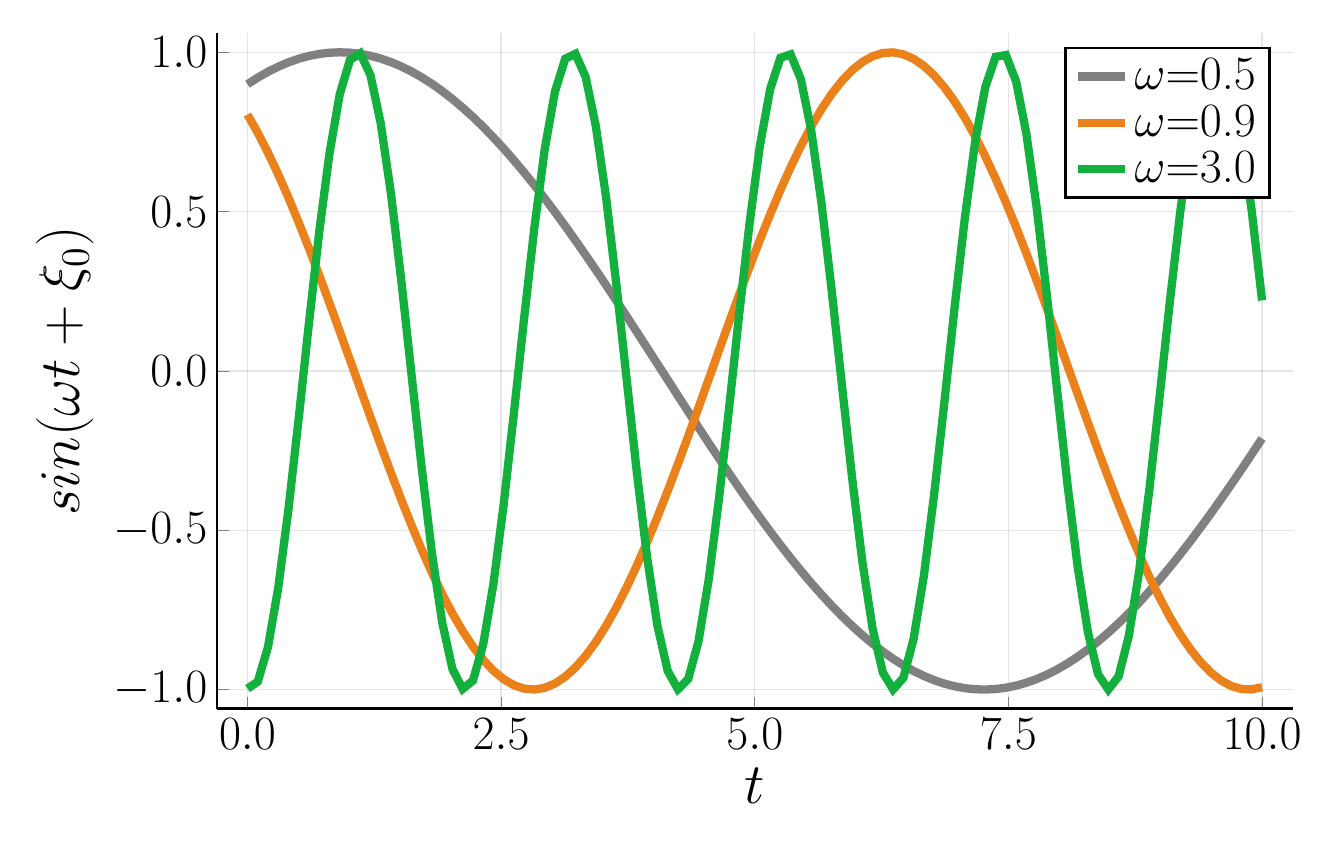
\begin{tikzpicture}[]
\begin{axis}[height = {101.6mm}, ylabel = {$\text{sin}(\omega t + \xi_0)$}, xmin = {-0.3}, xmax = {10.3}, ymax = {1.0599982810020447}, xlabel = {$t$}, unbounded coords=jump,scaled x ticks = false,xlabel style = {font = {\fontsize{22 pt}{28.6 pt}\selectfont}, color = {rgb,1:red,0.00000000;green,0.00000000;blue,0.00000000}, draw opacity = 1.0, rotate = 0.0},xmajorgrids = true,xtick = {0.0,2.5,5.0,7.5,10.0},xticklabels = {$0.0$,$2.5$,$5.0$,$7.5$,$10.0$},xtick align = inside,xticklabel style = {font = {\fontsize{16 pt}{20.8 pt}\selectfont}, color = {rgb,1:red,0.00000000;green,0.00000000;blue,0.00000000}, draw opacity = 1.0, rotate = 0.0},x grid style = {color = {rgb,1:red,0.00000000;green,0.00000000;blue,0.00000000},
draw opacity = 0.1,
line width = 0.5,
solid},axis x line* = left,x axis line style = {color = {rgb,1:red,0.00000000;green,0.00000000;blue,0.00000000},
draw opacity = 1.0,
line width = 1,
solid},scaled y ticks = false,ylabel style = {font = {\fontsize{22 pt}{28.6 pt}\selectfont}, color = {rgb,1:red,0.00000000;green,0.00000000;blue,0.00000000}, draw opacity = 1.0, rotate = 0.0},ymajorgrids = true,ytick = {-1.0,-0.5,0.0,0.5,1.0},yticklabels = {$-1.0$,$-0.5$,$0.0$,$0.5$,$1.0$},ytick align = inside,yticklabel style = {font = {\fontsize{16 pt}{20.8 pt}\selectfont}, color = {rgb,1:red,0.00000000;green,0.00000000;blue,0.00000000}, draw opacity = 1.0, rotate = 0.0},y grid style = {color = {rgb,1:red,0.00000000;green,0.00000000;blue,0.00000000},
draw opacity = 0.1,
line width = 0.5,
solid},axis y line* = left,y axis line style = {color = {rgb,1:red,0.00000000;green,0.00000000;blue,0.00000000},
draw opacity = 1.0,
line width = 1,
solid},    xshift = 0.0mm,
    yshift = 0.0mm,
    axis background/.style={fill={rgb,1:red,1.00000000;green,1.00000000;blue,1.00000000}}
,legend style = {color = {rgb,1:red,0.00000000;green,0.00000000;blue,0.00000000},
draw opacity = 1.0,
line width = 1,
solid,fill = {rgb,1:red,1.00000000;green,1.00000000;blue,1.00000000},font = {\fontsize{16 pt}{20.8 pt}\selectfont}},colorbar style={title=}, ymin = {-1.0599746775627137}, width = {152.4mm}]\addplot+ [color = {rgb,1:red,0.50196078;green,0.50196078;blue,0.50196078},
draw opacity = 1.0,
line width = 3,
solid,mark = none,
mark size = 2.0,
mark options = {
    color = {rgb,1:red,0.00000000;green,0.00000000;blue,0.00000000}, draw opacity = 1.0,
    fill = {rgb,1:red,0.50196078;green,0.50196078;blue,0.50196078}, fill opacity = 1.0,
    line width = 1,
    rotate = 0,
    solid
}]coordinates {
(0.0, 0.899838924407959)
(0.10101010101010101, 0.9205163717269897)
(0.20202020202020202, 0.9388930201530457)
(0.30303030303030304, 0.9549229145050049)
(0.40404040404040403, 0.9685660600662231)
(0.5050505050505051, 0.9797882437705994)
(0.6060606060606061, 0.9885614514350891)
(0.7070707070707071, 0.9948638081550598)
(0.8080808080808081, 0.998679518699646)
(0.9090909090909091, 0.9999990463256836)
(1.0101010101010102, 0.9988190531730652)
(1.1111111111111112, 0.9951425790786743)
(1.2121212121212122, 0.9889787435531616)
(1.3131313131313131, 0.9803429841995239)
(1.4141414141414141, 0.9692569375038147)
(1.5151515151515151, 0.9557482004165649)
(1.6161616161616161, 0.9398505687713623)
(1.7171717171717171, 0.921603798866272)
(1.8181818181818181, 0.9010535478591919)
(1.9191919191919191, 0.8782510757446289)
(2.0202020202020203, 0.8532534837722778)
(2.121212121212121, 0.8261231780052185)
(2.2222222222222223, 0.7969279885292053)
(2.323232323232323, 0.7657409310340881)
(2.4242424242424243, 0.7326399087905884)
(2.525252525252525, 0.6977076530456543)
(2.6262626262626263, 0.6610314846038818)
(2.727272727272727, 0.6227030754089355)
(2.8282828282828283, 0.5828182697296143)
(2.9292929292929295, 0.5414766669273376)
(3.0303030303030303, 0.4987817108631134)
(3.1313131313131315, 0.4548400342464447)
(3.2323232323232323, 0.4097614884376526)
(3.3333333333333335, 0.36365875601768494)
(3.4343434343434343, 0.31664708256721497)
(3.5353535353535355, 0.2688439190387726)
(3.6363636363636362, 0.22036881744861603)
(3.7373737373737375, 0.1713429093360901)
(3.8383838383838382, 0.12188872694969177)
(3.9393939393939394, 0.07212988287210464)
(4.040404040404041, 0.022190751507878304)
(4.141414141414141, -0.02780384197831154)
(4.242424242424242, -0.07772894203662872)
(4.343434343434343, -0.12745976448059082)
(4.444444444444445, -0.17687200009822845)
(4.545454545454546, -0.22584214806556702)
(4.646464646464646, -0.27424779534339905)
(4.747474747474747, -0.3219679892063141)
(4.848484848484849, -0.3688834011554718)
(4.94949494949495, -0.4148768186569214)
(5.05050505050505, -0.4598332643508911)
(5.151515151515151, -0.503640353679657)
(5.252525252525253, -0.5461885929107666)
(5.353535353535354, -0.5873717069625854)
(5.454545454545454, -0.6270866394042969)
(5.555555555555555, -0.6652342081069946)
(5.656565656565657, -0.7017189860343933)
(5.757575757575758, -0.7364498972892761)
(5.858585858585859, -0.7693400382995605)
(5.959595959595959, -0.8003072142601013)
(6.0606060606060606, -0.82927405834198)
(6.161616161616162, -0.8561681509017944)
(6.262626262626263, -0.880922257900238)
(6.363636363636363, -0.9034745097160339)
(6.4646464646464645, -0.9237685799598694)
(6.565656565656566, -0.9417536854743958)
(6.666666666666667, -0.9573848843574524)
(6.767676767676767, -0.9706231951713562)
(6.8686868686868685, -0.9814353585243225)
(6.96969696969697, -0.9897944927215576)
(7.070707070707071, -0.9956796169281006)
(7.171717171717172, -0.9990761280059814)
(7.2727272727272725, -0.9999754428863525)
(7.373737373737374, -0.9983752965927124)
(7.474747474747475, -0.9942798018455505)
(7.575757575757576, -0.987699031829834)
(7.6767676767676765, -0.9786496162414551)
(7.777777777777778, -0.9671540260314941)
(7.878787878787879, -0.9532411098480225)
(7.97979797979798, -0.9369455575942993)
(8.080808080808081, -0.9183081388473511)
(8.181818181818182, -0.8973754048347473)
(8.282828282828282, -0.8741997480392456)
(8.383838383838384, -0.8488389849662781)
(8.484848484848484, -0.8213565945625305)
(8.585858585858587, -0.7918212413787842)
(8.686868686868687, -0.7603067755699158)
(8.787878787878787, -0.7268918752670288)
(8.88888888888889, -0.6916601657867432)
(8.98989898989899, -0.6546996831893921)
(9.090909090909092, -0.6161027550697327)
(9.191919191919192, -0.5759658813476562)
(9.292929292929292, -0.5343894362449646)
(9.393939393939394, -0.49147728085517883)
(9.494949494949495, -0.44733667373657227)
(9.595959595959595, -0.40207797288894653)
(9.696969696969697, -0.35581427812576294)
(9.797979797979798, -0.30866125226020813)
(9.8989898989899, -0.26073670387268066)
(10.0, -0.21216046810150146)
};
\addlegendentry{$\omega$=0.5}
\addplot+ [color = {rgb,1:red,0.92156863;green,0.50588235;blue,0.10588235},
draw opacity = 1.0,
line width = 3,
solid,mark = none,
mark size = 2.0,
mark options = {
    color = {rgb,1:red,0.00000000;green,0.00000000;blue,0.00000000}, draw opacity = 1.0,
    fill = {rgb,1:red,0.92156863;green,0.50588235;blue,0.10588235}, fill opacity = 1.0,
    line width = 1,
    rotate = 0,
    solid
}]coordinates {
(0.0, 0.8044089674949646)
(0.10101010101010101, 0.7477586269378662)
(0.20202020202020202, 0.6850554943084717)
(0.30303030303030304, 0.616807222366333)
(0.40404040404040403, 0.543566107749939)
(0.5050505050505051, 0.4659251570701599)
(0.6060606060606061, 0.384512722492218)
(0.7070707070707071, 0.2999878227710724)
(0.8080808080808081, 0.21303468942642212)
(0.9090909090909091, 0.12435712665319443)
(1.0101010101010102, 0.034672949463129044)
(1.1111111111111112, -0.05529188737273216)
(1.2121212121212122, -0.14480917155742645)
(1.3131313131313131, -0.2331542819738388)
(1.4141414141414141, -0.3196121156215668)
(1.5151515151515151, -0.4034828245639801)
(1.6161616161616161, -0.4840875566005707)
(1.7171717171717171, -0.5607737898826599)
(1.8181818181818181, -0.6329208612442017)
(1.9191919191919191, -0.6999447345733643)
(2.0202020202020203, -0.7613028287887573)
(2.121212121212121, -0.8164985775947571)
(2.2222222222222223, -0.8650851249694824)
(2.323232323232323, -0.9066692590713501)
(2.4242424242424243, -0.9409142732620239)
(2.525252525252525, -0.9675430655479431)
(2.6262626262626263, -0.9863400459289551)
(2.727272727272727, -0.9971530437469482)
(2.8282828282828283, -0.9998945593833923)
(2.9292929292929295, -0.9945423603057861)
(3.0303030303030303, -0.9811398386955261)
(3.1313131313131315, -0.9597954154014587)
(3.2323232323232323, -0.9306819438934326)
(3.3333333333333335, -0.8940350413322449)
(3.4343434343434343, -0.8501513004302979)
(3.5353535353535355, -0.7993859648704529)
(3.6363636363636362, -0.7421500086784363)
(3.7373737373737375, -0.6789066791534424)
(3.8383838383838382, -0.610167920589447)
(3.9393939393939394, -0.5364901423454285)
(4.040404040404041, -0.4584697484970093)
(4.141414141414141, -0.37673822045326233)
(4.242424242424242, -0.29195719957351685)
(4.343434343434343, -0.2048128992319107)
(4.444444444444445, -0.11601074039936066)
(4.545454545454546, -0.02626953087747097)
(4.646464646464646, 0.06368432193994522)
(4.747474747474747, 0.153122678399086)
(4.848484848484849, 0.24132157862186432)
(4.94949494949495, 0.32756710052490234)
(5.05050505050505, 0.4111610949039459)
(5.151515151515151, 0.491426944732666)
(5.252525252525253, 0.5677149295806885)
(5.353535353535354, 0.6394075155258179)
(5.454545454545454, 0.705924391746521)
(5.555555555555555, 0.7667271494865417)
(5.656565656565657, 0.8213236331939697)
(5.757575757575758, 0.8692718744277954)
(5.858585858585859, 0.9101837277412415)
(5.959595959595959, 0.9437280893325806)
(6.0606060606060606, 0.9696334004402161)
(6.161616161616162, 0.9876900315284729)
(6.262626262626263, 0.9977517127990723)
(6.363636363636363, 0.9997370839118958)
(6.4646464646464645, 0.993630051612854)
(6.565656565656566, 0.9794800281524658)
(6.666666666666667, 0.9574015736579895)
(6.767676767676767, 0.9275734424591064)
(6.8686868686868685, 0.8902369737625122)
(6.96969696969697, 0.8456944823265076)
(7.070707070707071, 0.7943065166473389)
(7.171717171717172, 0.7364889979362488)
(7.2727272727272725, 0.6727098822593689)
(7.373737373737374, 0.6034855246543884)
(7.474747474747475, 0.5293762683868408)
(7.575757575757576, 0.4509819447994232)
(7.6767676767676765, 0.36893710494041443)
(7.777777777777778, 0.28390592336654663)
(7.878787878787879, 0.19657664000988007)
(7.97979797979798, 0.10765615850687027)
(8.080808080808081, 0.017864255234599113)
(8.181818181818182, -0.07207225263118744)
(8.282828282828282, -0.1614253669977188)
(8.383838383838384, -0.24947182834148407)
(8.484848484848484, -0.3354989290237427)
(8.585858585858587, -0.41881030797958374)
(8.686868686868687, -0.4987316131591797)
(8.787878787878787, -0.5746159553527832)
(8.88888888888889, -0.6458489894866943)
(8.98989898989899, -0.7118542194366455)
(9.090909090909092, -0.7720972895622253)
(9.191919191919192, -0.8260906338691711)
(9.292929292929292, -0.8733971118927002)
(9.393939393939394, -0.9136338829994202)
(9.494949494949495, -0.9464752078056335)
(9.595959595959595, -0.9716552495956421)
(9.696969696969697, -0.9889702200889587)
(9.797979797979798, -0.9982799291610718)
(9.8989898989899, -0.9995089769363403)
(10.0, -0.9926475286483765)
};
\addlegendentry{$\omega$=0.9}
\addplot+ [color = {rgb,1:red,0.07843137;green,0.69019608;blue,0.23921569},
draw opacity = 1.0,
line width = 3,
solid,mark = none,
mark size = 2.0,
mark options = {
    color = {rgb,1:red,0.00000000;green,0.00000000;blue,0.00000000}, draw opacity = 1.0,
    fill = {rgb,1:red,0.07843137;green,0.69019608;blue,0.23921569}, fill opacity = 1.0,
    line width = 1,
    rotate = 0,
    solid
}]coordinates {
(0.0, -0.9969542622566223)
(0.10101010101010101, -0.9754739999771118)
(0.20202020202020202, -0.866857647895813)
(0.30303030303030304, -0.6808074116706848)
(0.40404040404040403, -0.4339427053928375)
(0.5050505050505051, -0.1483151912689209)
(0.6060606060606061, 0.1505608856678009)
(0.7070707070707071, 0.43598780035972595)
(0.8080808080808081, 0.6824692487716675)
(0.9090909090909091, 0.8679876923561096)
(1.0101010101010102, 0.9759714603424072)
(1.1111111111111112, 0.9967745542526245)
(1.2121212121212122, 0.9285387396812439)
(1.3131313131313131, 0.7773593664169312)
(1.4141414141414141, 0.5567407608032227)
(1.5151515151515151, 0.28639015555381775)
(1.6161616161616161, -0.009542805142700672)
(1.7171717171717171, -0.3046233355998993)
(1.8181818181818181, -0.572492778301239)
(1.9191919191919191, -0.7892231345176697)
(2.0202020202020203, -0.9354545474052429)
(2.121212121212121, -0.9981245994567871)
(2.2222222222222223, -0.9716351628303528)
(2.323232323232323, -0.8583524227142334)
(2.4242424242424243, -0.6683956384658813)
(2.525252525252525, -0.41873303055763245)
(2.6262626262626263, -0.13166627287864685)
(2.727272727272727, 0.16716183722019196)
(2.8282828282828283, 0.45105788111686707)
(2.9292929292929295, 0.6946622729301453)
(3.0303030303030303, 0.8762145638465881)
(3.1313131313131315, 0.9794971942901611)
(3.2323232323232323, 0.9952842593193054)
(3.3333333333333335, 0.92216557264328)
(3.4343434343434343, 0.7666725516319275)
(3.5353535353535355, 0.5426949858665466)
(3.6363636363636362, 0.27024006843566895)
(3.7373737373737375, -0.02635459043085575)
(3.8383838383838382, -0.32059505581855774)
(3.9393939393939394, -0.5861977338790894)
(4.040404040404041, -0.7994371056556702)
(4.141414141414141, -0.9412651658058167)
(4.242424242424242, -0.9990127682685852)
(4.343434343434343, -0.9675215482711792)
(4.444444444444445, -0.8496045470237732)
(4.545454545454546, -0.6557948589324951)
(4.646464646464646, -0.40340498089790344)
(4.747474747474747, -0.11498014628887177)
(4.848484848484849, 0.18371552228927612)
(4.94949494949495, 0.46600043773651123)
(5.05050505050505, 0.7066588997840881)
(5.151515151515151, 0.8841936588287354)
(5.252525252525253, 0.9827460050582886)
(5.353535353535354, 0.9935125708580017)
(5.454545454545454, 0.9155316352844238)
(5.555555555555555, 0.7557690143585205)
(5.656565656565657, 0.528495728969574)
(5.757575757575758, 0.2540135383605957)
(5.858585858585859, -0.04315892606973648)
(5.959595959595959, -0.3364761471748352)
(6.0606060606060606, -0.5997369289398193)
(6.161616161616162, -0.8094250559806824)
(6.262626262626263, -0.9468095898628235)
(6.363636363636363, -0.9996184706687927)
(6.4646464646464645, -0.9631344079971313)
(6.565656565656566, -0.8406164050102234)
(6.666666666666667, -0.6430086493492126)
(6.767676767676767, -0.38796287775039673)
(6.8686868686868685, -0.0982615053653717)
(6.96969696969697, 0.20021727681159973)
(7.070707070707071, 0.4808112382888794)
(7.171717171717172, 0.7184557914733887)
(7.2727272727272725, 0.8919227719306946)
(7.373737373737374, 0.9857169985771179)
(7.474747474747475, 0.9914600253105164)
(7.575757575757576, 0.9086388945579529)
(7.6767676767676765, 0.7446517944335938)
(7.777777777777778, 0.5141471028327942)
(7.878787878787879, 0.2377152293920517)
(7.97979797979798, -0.0599510595202446)
(8.080808080808081, -0.35226207971572876)
(8.181818181818182, -0.6131066083908081)
(8.282828282828282, -0.8191841244697571)
(8.383838383838384, -0.9520863890647888)
(8.484848484848484, -0.9999415874481201)
(8.585858585858587, -0.9584749937057495)
(8.686868686868687, -0.8313906788825989)
(8.787878787878787, -0.63004070520401)
(8.88888888888889, -0.3724110722541809)
(8.98989898989899, -0.08151508122682571)
(9.090909090909092, 0.2166624218225479)
(9.191919191919192, 0.4954861104488373)
(9.292929292929292, 0.7300494909286499)
(9.393939393939394, 0.8993997573852539)
(9.494949494949495, 0.9884092807769775)
(9.595959595959595, 0.9891271591186523)
(9.696969696969697, 0.9014892578125)
(9.797979797979798, 0.7333239912986755)
(9.8989898989899, 0.4996531307697296)
(10.0, 0.22134970128536224)
};
\addlegendentry{$\omega$=3.0}
\end{axis}

\end{tikzpicture}
}
  \begin{block}{The simplified problem}
    \begin{itemize}
      \item Learn generating model of harmonic signals
      \item varying frequency $\omega$ and phase $\xi_0$
      %\item ODE: $\ddot\xi = -\omega^2 \xi$
    \end{itemize}
  \end{block}
\end{frame}



\begin{frame}{Outline}
  \begin{enumerate}
    \item \alert{Explainability} via ODEs
    \item \alert{Sparsity} of the ODE via \emph{Automatic Relevance Determination} (ARD)
    \item \alert{Generative Models} for manifold learning
  \end{enumerate}
\end{frame}
\note{
  \begin{itemize}
    \item ODE because physicists like them
    \item sparsity for simplicity (occam's razor)
  \end{itemize}
}

\sectionpic{Ordinary differential equations}{
  $$
    \frac{\partial \bm\xi}{\partial t} = f(\bm \xi, \bm\theta, t) \approx \bm W \bm\xi + \bm b
  $$
}
\note{
  \begin{itemize}
    \item ODE: diff eq. with one variable $\xi$
    \item we can use vectorized from to represent nth order ODE: $W\xi+b$
    \item parameters $W$,$b$ are (almost) intuitively interpretable
  \end{itemize}
}

\begin{frame}{Example: Harmonic oscillator}
  \centering
  \resizebox{!}{.4\textwidth}{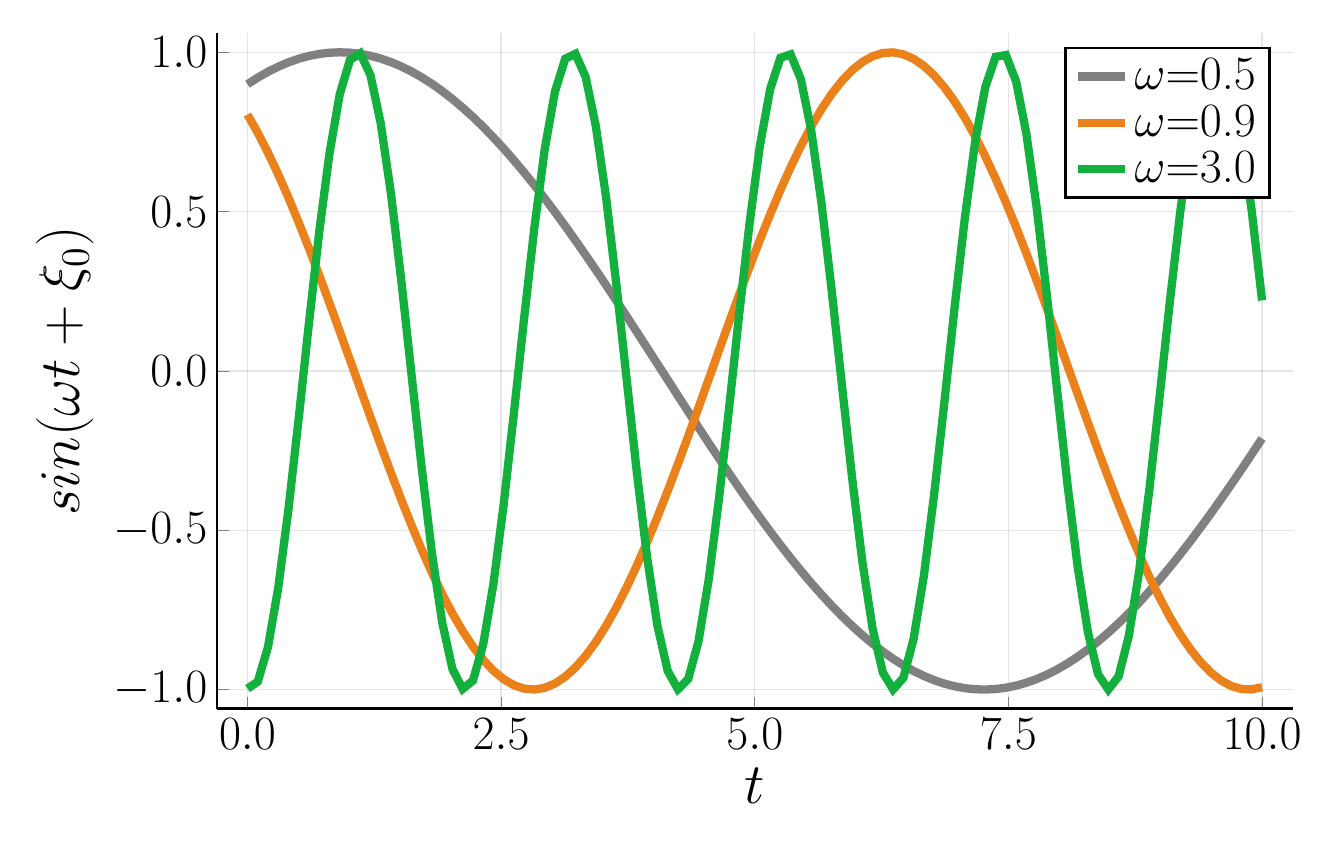
\begin{tikzpicture}[]
\begin{axis}[height = {101.6mm}, ylabel = {$\text{sin}(\omega t + \xi_0)$}, xmin = {-0.3}, xmax = {10.3}, ymax = {1.0599982810020447}, xlabel = {$t$}, unbounded coords=jump,scaled x ticks = false,xlabel style = {font = {\fontsize{22 pt}{28.6 pt}\selectfont}, color = {rgb,1:red,0.00000000;green,0.00000000;blue,0.00000000}, draw opacity = 1.0, rotate = 0.0},xmajorgrids = true,xtick = {0.0,2.5,5.0,7.5,10.0},xticklabels = {$0.0$,$2.5$,$5.0$,$7.5$,$10.0$},xtick align = inside,xticklabel style = {font = {\fontsize{16 pt}{20.8 pt}\selectfont}, color = {rgb,1:red,0.00000000;green,0.00000000;blue,0.00000000}, draw opacity = 1.0, rotate = 0.0},x grid style = {color = {rgb,1:red,0.00000000;green,0.00000000;blue,0.00000000},
draw opacity = 0.1,
line width = 0.5,
solid},axis x line* = left,x axis line style = {color = {rgb,1:red,0.00000000;green,0.00000000;blue,0.00000000},
draw opacity = 1.0,
line width = 1,
solid},scaled y ticks = false,ylabel style = {font = {\fontsize{22 pt}{28.6 pt}\selectfont}, color = {rgb,1:red,0.00000000;green,0.00000000;blue,0.00000000}, draw opacity = 1.0, rotate = 0.0},ymajorgrids = true,ytick = {-1.0,-0.5,0.0,0.5,1.0},yticklabels = {$-1.0$,$-0.5$,$0.0$,$0.5$,$1.0$},ytick align = inside,yticklabel style = {font = {\fontsize{16 pt}{20.8 pt}\selectfont}, color = {rgb,1:red,0.00000000;green,0.00000000;blue,0.00000000}, draw opacity = 1.0, rotate = 0.0},y grid style = {color = {rgb,1:red,0.00000000;green,0.00000000;blue,0.00000000},
draw opacity = 0.1,
line width = 0.5,
solid},axis y line* = left,y axis line style = {color = {rgb,1:red,0.00000000;green,0.00000000;blue,0.00000000},
draw opacity = 1.0,
line width = 1,
solid},    xshift = 0.0mm,
    yshift = 0.0mm,
    axis background/.style={fill={rgb,1:red,1.00000000;green,1.00000000;blue,1.00000000}}
,legend style = {color = {rgb,1:red,0.00000000;green,0.00000000;blue,0.00000000},
draw opacity = 1.0,
line width = 1,
solid,fill = {rgb,1:red,1.00000000;green,1.00000000;blue,1.00000000},font = {\fontsize{16 pt}{20.8 pt}\selectfont}},colorbar style={title=}, ymin = {-1.0599746775627137}, width = {152.4mm}]\addplot+ [color = {rgb,1:red,0.50196078;green,0.50196078;blue,0.50196078},
draw opacity = 1.0,
line width = 3,
solid,mark = none,
mark size = 2.0,
mark options = {
    color = {rgb,1:red,0.00000000;green,0.00000000;blue,0.00000000}, draw opacity = 1.0,
    fill = {rgb,1:red,0.50196078;green,0.50196078;blue,0.50196078}, fill opacity = 1.0,
    line width = 1,
    rotate = 0,
    solid
}]coordinates {
(0.0, 0.899838924407959)
(0.10101010101010101, 0.9205163717269897)
(0.20202020202020202, 0.9388930201530457)
(0.30303030303030304, 0.9549229145050049)
(0.40404040404040403, 0.9685660600662231)
(0.5050505050505051, 0.9797882437705994)
(0.6060606060606061, 0.9885614514350891)
(0.7070707070707071, 0.9948638081550598)
(0.8080808080808081, 0.998679518699646)
(0.9090909090909091, 0.9999990463256836)
(1.0101010101010102, 0.9988190531730652)
(1.1111111111111112, 0.9951425790786743)
(1.2121212121212122, 0.9889787435531616)
(1.3131313131313131, 0.9803429841995239)
(1.4141414141414141, 0.9692569375038147)
(1.5151515151515151, 0.9557482004165649)
(1.6161616161616161, 0.9398505687713623)
(1.7171717171717171, 0.921603798866272)
(1.8181818181818181, 0.9010535478591919)
(1.9191919191919191, 0.8782510757446289)
(2.0202020202020203, 0.8532534837722778)
(2.121212121212121, 0.8261231780052185)
(2.2222222222222223, 0.7969279885292053)
(2.323232323232323, 0.7657409310340881)
(2.4242424242424243, 0.7326399087905884)
(2.525252525252525, 0.6977076530456543)
(2.6262626262626263, 0.6610314846038818)
(2.727272727272727, 0.6227030754089355)
(2.8282828282828283, 0.5828182697296143)
(2.9292929292929295, 0.5414766669273376)
(3.0303030303030303, 0.4987817108631134)
(3.1313131313131315, 0.4548400342464447)
(3.2323232323232323, 0.4097614884376526)
(3.3333333333333335, 0.36365875601768494)
(3.4343434343434343, 0.31664708256721497)
(3.5353535353535355, 0.2688439190387726)
(3.6363636363636362, 0.22036881744861603)
(3.7373737373737375, 0.1713429093360901)
(3.8383838383838382, 0.12188872694969177)
(3.9393939393939394, 0.07212988287210464)
(4.040404040404041, 0.022190751507878304)
(4.141414141414141, -0.02780384197831154)
(4.242424242424242, -0.07772894203662872)
(4.343434343434343, -0.12745976448059082)
(4.444444444444445, -0.17687200009822845)
(4.545454545454546, -0.22584214806556702)
(4.646464646464646, -0.27424779534339905)
(4.747474747474747, -0.3219679892063141)
(4.848484848484849, -0.3688834011554718)
(4.94949494949495, -0.4148768186569214)
(5.05050505050505, -0.4598332643508911)
(5.151515151515151, -0.503640353679657)
(5.252525252525253, -0.5461885929107666)
(5.353535353535354, -0.5873717069625854)
(5.454545454545454, -0.6270866394042969)
(5.555555555555555, -0.6652342081069946)
(5.656565656565657, -0.7017189860343933)
(5.757575757575758, -0.7364498972892761)
(5.858585858585859, -0.7693400382995605)
(5.959595959595959, -0.8003072142601013)
(6.0606060606060606, -0.82927405834198)
(6.161616161616162, -0.8561681509017944)
(6.262626262626263, -0.880922257900238)
(6.363636363636363, -0.9034745097160339)
(6.4646464646464645, -0.9237685799598694)
(6.565656565656566, -0.9417536854743958)
(6.666666666666667, -0.9573848843574524)
(6.767676767676767, -0.9706231951713562)
(6.8686868686868685, -0.9814353585243225)
(6.96969696969697, -0.9897944927215576)
(7.070707070707071, -0.9956796169281006)
(7.171717171717172, -0.9990761280059814)
(7.2727272727272725, -0.9999754428863525)
(7.373737373737374, -0.9983752965927124)
(7.474747474747475, -0.9942798018455505)
(7.575757575757576, -0.987699031829834)
(7.6767676767676765, -0.9786496162414551)
(7.777777777777778, -0.9671540260314941)
(7.878787878787879, -0.9532411098480225)
(7.97979797979798, -0.9369455575942993)
(8.080808080808081, -0.9183081388473511)
(8.181818181818182, -0.8973754048347473)
(8.282828282828282, -0.8741997480392456)
(8.383838383838384, -0.8488389849662781)
(8.484848484848484, -0.8213565945625305)
(8.585858585858587, -0.7918212413787842)
(8.686868686868687, -0.7603067755699158)
(8.787878787878787, -0.7268918752670288)
(8.88888888888889, -0.6916601657867432)
(8.98989898989899, -0.6546996831893921)
(9.090909090909092, -0.6161027550697327)
(9.191919191919192, -0.5759658813476562)
(9.292929292929292, -0.5343894362449646)
(9.393939393939394, -0.49147728085517883)
(9.494949494949495, -0.44733667373657227)
(9.595959595959595, -0.40207797288894653)
(9.696969696969697, -0.35581427812576294)
(9.797979797979798, -0.30866125226020813)
(9.8989898989899, -0.26073670387268066)
(10.0, -0.21216046810150146)
};
\addlegendentry{$\omega$=0.5}
\addplot+ [color = {rgb,1:red,0.92156863;green,0.50588235;blue,0.10588235},
draw opacity = 1.0,
line width = 3,
solid,mark = none,
mark size = 2.0,
mark options = {
    color = {rgb,1:red,0.00000000;green,0.00000000;blue,0.00000000}, draw opacity = 1.0,
    fill = {rgb,1:red,0.92156863;green,0.50588235;blue,0.10588235}, fill opacity = 1.0,
    line width = 1,
    rotate = 0,
    solid
}]coordinates {
(0.0, 0.8044089674949646)
(0.10101010101010101, 0.7477586269378662)
(0.20202020202020202, 0.6850554943084717)
(0.30303030303030304, 0.616807222366333)
(0.40404040404040403, 0.543566107749939)
(0.5050505050505051, 0.4659251570701599)
(0.6060606060606061, 0.384512722492218)
(0.7070707070707071, 0.2999878227710724)
(0.8080808080808081, 0.21303468942642212)
(0.9090909090909091, 0.12435712665319443)
(1.0101010101010102, 0.034672949463129044)
(1.1111111111111112, -0.05529188737273216)
(1.2121212121212122, -0.14480917155742645)
(1.3131313131313131, -0.2331542819738388)
(1.4141414141414141, -0.3196121156215668)
(1.5151515151515151, -0.4034828245639801)
(1.6161616161616161, -0.4840875566005707)
(1.7171717171717171, -0.5607737898826599)
(1.8181818181818181, -0.6329208612442017)
(1.9191919191919191, -0.6999447345733643)
(2.0202020202020203, -0.7613028287887573)
(2.121212121212121, -0.8164985775947571)
(2.2222222222222223, -0.8650851249694824)
(2.323232323232323, -0.9066692590713501)
(2.4242424242424243, -0.9409142732620239)
(2.525252525252525, -0.9675430655479431)
(2.6262626262626263, -0.9863400459289551)
(2.727272727272727, -0.9971530437469482)
(2.8282828282828283, -0.9998945593833923)
(2.9292929292929295, -0.9945423603057861)
(3.0303030303030303, -0.9811398386955261)
(3.1313131313131315, -0.9597954154014587)
(3.2323232323232323, -0.9306819438934326)
(3.3333333333333335, -0.8940350413322449)
(3.4343434343434343, -0.8501513004302979)
(3.5353535353535355, -0.7993859648704529)
(3.6363636363636362, -0.7421500086784363)
(3.7373737373737375, -0.6789066791534424)
(3.8383838383838382, -0.610167920589447)
(3.9393939393939394, -0.5364901423454285)
(4.040404040404041, -0.4584697484970093)
(4.141414141414141, -0.37673822045326233)
(4.242424242424242, -0.29195719957351685)
(4.343434343434343, -0.2048128992319107)
(4.444444444444445, -0.11601074039936066)
(4.545454545454546, -0.02626953087747097)
(4.646464646464646, 0.06368432193994522)
(4.747474747474747, 0.153122678399086)
(4.848484848484849, 0.24132157862186432)
(4.94949494949495, 0.32756710052490234)
(5.05050505050505, 0.4111610949039459)
(5.151515151515151, 0.491426944732666)
(5.252525252525253, 0.5677149295806885)
(5.353535353535354, 0.6394075155258179)
(5.454545454545454, 0.705924391746521)
(5.555555555555555, 0.7667271494865417)
(5.656565656565657, 0.8213236331939697)
(5.757575757575758, 0.8692718744277954)
(5.858585858585859, 0.9101837277412415)
(5.959595959595959, 0.9437280893325806)
(6.0606060606060606, 0.9696334004402161)
(6.161616161616162, 0.9876900315284729)
(6.262626262626263, 0.9977517127990723)
(6.363636363636363, 0.9997370839118958)
(6.4646464646464645, 0.993630051612854)
(6.565656565656566, 0.9794800281524658)
(6.666666666666667, 0.9574015736579895)
(6.767676767676767, 0.9275734424591064)
(6.8686868686868685, 0.8902369737625122)
(6.96969696969697, 0.8456944823265076)
(7.070707070707071, 0.7943065166473389)
(7.171717171717172, 0.7364889979362488)
(7.2727272727272725, 0.6727098822593689)
(7.373737373737374, 0.6034855246543884)
(7.474747474747475, 0.5293762683868408)
(7.575757575757576, 0.4509819447994232)
(7.6767676767676765, 0.36893710494041443)
(7.777777777777778, 0.28390592336654663)
(7.878787878787879, 0.19657664000988007)
(7.97979797979798, 0.10765615850687027)
(8.080808080808081, 0.017864255234599113)
(8.181818181818182, -0.07207225263118744)
(8.282828282828282, -0.1614253669977188)
(8.383838383838384, -0.24947182834148407)
(8.484848484848484, -0.3354989290237427)
(8.585858585858587, -0.41881030797958374)
(8.686868686868687, -0.4987316131591797)
(8.787878787878787, -0.5746159553527832)
(8.88888888888889, -0.6458489894866943)
(8.98989898989899, -0.7118542194366455)
(9.090909090909092, -0.7720972895622253)
(9.191919191919192, -0.8260906338691711)
(9.292929292929292, -0.8733971118927002)
(9.393939393939394, -0.9136338829994202)
(9.494949494949495, -0.9464752078056335)
(9.595959595959595, -0.9716552495956421)
(9.696969696969697, -0.9889702200889587)
(9.797979797979798, -0.9982799291610718)
(9.8989898989899, -0.9995089769363403)
(10.0, -0.9926475286483765)
};
\addlegendentry{$\omega$=0.9}
\addplot+ [color = {rgb,1:red,0.07843137;green,0.69019608;blue,0.23921569},
draw opacity = 1.0,
line width = 3,
solid,mark = none,
mark size = 2.0,
mark options = {
    color = {rgb,1:red,0.00000000;green,0.00000000;blue,0.00000000}, draw opacity = 1.0,
    fill = {rgb,1:red,0.07843137;green,0.69019608;blue,0.23921569}, fill opacity = 1.0,
    line width = 1,
    rotate = 0,
    solid
}]coordinates {
(0.0, -0.9969542622566223)
(0.10101010101010101, -0.9754739999771118)
(0.20202020202020202, -0.866857647895813)
(0.30303030303030304, -0.6808074116706848)
(0.40404040404040403, -0.4339427053928375)
(0.5050505050505051, -0.1483151912689209)
(0.6060606060606061, 0.1505608856678009)
(0.7070707070707071, 0.43598780035972595)
(0.8080808080808081, 0.6824692487716675)
(0.9090909090909091, 0.8679876923561096)
(1.0101010101010102, 0.9759714603424072)
(1.1111111111111112, 0.9967745542526245)
(1.2121212121212122, 0.9285387396812439)
(1.3131313131313131, 0.7773593664169312)
(1.4141414141414141, 0.5567407608032227)
(1.5151515151515151, 0.28639015555381775)
(1.6161616161616161, -0.009542805142700672)
(1.7171717171717171, -0.3046233355998993)
(1.8181818181818181, -0.572492778301239)
(1.9191919191919191, -0.7892231345176697)
(2.0202020202020203, -0.9354545474052429)
(2.121212121212121, -0.9981245994567871)
(2.2222222222222223, -0.9716351628303528)
(2.323232323232323, -0.8583524227142334)
(2.4242424242424243, -0.6683956384658813)
(2.525252525252525, -0.41873303055763245)
(2.6262626262626263, -0.13166627287864685)
(2.727272727272727, 0.16716183722019196)
(2.8282828282828283, 0.45105788111686707)
(2.9292929292929295, 0.6946622729301453)
(3.0303030303030303, 0.8762145638465881)
(3.1313131313131315, 0.9794971942901611)
(3.2323232323232323, 0.9952842593193054)
(3.3333333333333335, 0.92216557264328)
(3.4343434343434343, 0.7666725516319275)
(3.5353535353535355, 0.5426949858665466)
(3.6363636363636362, 0.27024006843566895)
(3.7373737373737375, -0.02635459043085575)
(3.8383838383838382, -0.32059505581855774)
(3.9393939393939394, -0.5861977338790894)
(4.040404040404041, -0.7994371056556702)
(4.141414141414141, -0.9412651658058167)
(4.242424242424242, -0.9990127682685852)
(4.343434343434343, -0.9675215482711792)
(4.444444444444445, -0.8496045470237732)
(4.545454545454546, -0.6557948589324951)
(4.646464646464646, -0.40340498089790344)
(4.747474747474747, -0.11498014628887177)
(4.848484848484849, 0.18371552228927612)
(4.94949494949495, 0.46600043773651123)
(5.05050505050505, 0.7066588997840881)
(5.151515151515151, 0.8841936588287354)
(5.252525252525253, 0.9827460050582886)
(5.353535353535354, 0.9935125708580017)
(5.454545454545454, 0.9155316352844238)
(5.555555555555555, 0.7557690143585205)
(5.656565656565657, 0.528495728969574)
(5.757575757575758, 0.2540135383605957)
(5.858585858585859, -0.04315892606973648)
(5.959595959595959, -0.3364761471748352)
(6.0606060606060606, -0.5997369289398193)
(6.161616161616162, -0.8094250559806824)
(6.262626262626263, -0.9468095898628235)
(6.363636363636363, -0.9996184706687927)
(6.4646464646464645, -0.9631344079971313)
(6.565656565656566, -0.8406164050102234)
(6.666666666666667, -0.6430086493492126)
(6.767676767676767, -0.38796287775039673)
(6.8686868686868685, -0.0982615053653717)
(6.96969696969697, 0.20021727681159973)
(7.070707070707071, 0.4808112382888794)
(7.171717171717172, 0.7184557914733887)
(7.2727272727272725, 0.8919227719306946)
(7.373737373737374, 0.9857169985771179)
(7.474747474747475, 0.9914600253105164)
(7.575757575757576, 0.9086388945579529)
(7.6767676767676765, 0.7446517944335938)
(7.777777777777778, 0.5141471028327942)
(7.878787878787879, 0.2377152293920517)
(7.97979797979798, -0.0599510595202446)
(8.080808080808081, -0.35226207971572876)
(8.181818181818182, -0.6131066083908081)
(8.282828282828282, -0.8191841244697571)
(8.383838383838384, -0.9520863890647888)
(8.484848484848484, -0.9999415874481201)
(8.585858585858587, -0.9584749937057495)
(8.686868686868687, -0.8313906788825989)
(8.787878787878787, -0.63004070520401)
(8.88888888888889, -0.3724110722541809)
(8.98989898989899, -0.08151508122682571)
(9.090909090909092, 0.2166624218225479)
(9.191919191919192, 0.4954861104488373)
(9.292929292929292, 0.7300494909286499)
(9.393939393939394, 0.8993997573852539)
(9.494949494949495, 0.9884092807769775)
(9.595959595959595, 0.9891271591186523)
(9.696969696969697, 0.9014892578125)
(9.797979797979798, 0.7333239912986755)
(9.8989898989899, 0.4996531307697296)
(10.0, 0.22134970128536224)
};
\addlegendentry{$\omega$=3.0}
\end{axis}

\end{tikzpicture}
}
  \begin{minipage}{.49\textwidth}
    \begin{block}{Scalar form}
    \begin{align*}
      \ddot{\xi} = -\omega^2\xi
    \end{align*}
    \vspace{.05cm}
    \end{block}
  \end{minipage}
  \begin{minipage}{.49\textwidth}
    \begin{block}{Matrix form}
      \begin{align*}
        \begin{bmatrix}
          \dot{\xi} \\ \ddot{\xi}
        \end{bmatrix}
        =
        \begin{bmatrix}
          0 & 1\\
          -\omega^2 & 0\\
        \end{bmatrix}
        \begin{bmatrix}
          \xi \\ \dot{\xi}
        \end{bmatrix}
        +
        \begin{bmatrix}
          0 \\ 0
        \end{bmatrix}
      \end{align*}
    \end{block}
  \end{minipage}
\end{frame}
\note{
  \begin{itemize}
    \item Attempt: learn right box only from \textbf{partial obs}.
    \item that means: sparsity, $1$, $\omega$, $\xi$, $\dot\xi$
    \item awesome toy problem! (const, spec, zeros)
  \end{itemize}
}

\begin{frame}{Odent - VAE + ODE solver}
  \centering
  \def\layersep{2.6cm}
  \begin{tikzpicture}[shorten >=1pt,->,draw=black!50, node distance=\layersep]
    \tikzstyle{every pin edge}=[<-,shorten <=1pt]
    \tikzstyle{neuron}=[circle,fill=black!25,minimum size=17pt,inner sep=0pt]
    \tikzstyle{input neuron}=[neuron, fill=gray];
    \tikzstyle{output neuron}=[neuron, fill=gray];
    \tikzstyle{hidden neuron}=[neuron, fill=mLightBrown];
    \tikzstyle{annot} = [text width=4em, text centered]
  
    % Draw the hidden layer nodes
    \node[hidden neuron] (H-1) at (\layersep,-2cm) {$\bm W$};
    \node[hidden neuron] (H-2) at (\layersep,-3cm) {$\bm \xi$};
    \node[hidden neuron] (H-3) at (\layersep,-4cm) {$\bm b$};
  
    % Draw the output layer node
    \foreach \name / \y in {1,...,5}
        \node[output neuron] (O-\name) at (\layersep*2,-\y cm) {};
  
    % draw and connect decoder
    \node[draw, ultra thick, rotate=90, rounded corners=8, minimum height=1.1cm, minimum width=3.5cm]
        (odesolve) at  (\layersep+\layersep/2, -3) {ODE solver $\psi$};
    \foreach \name / \y in {1,...,3}
        \path (H-\name) edge (odesolve);
    \foreach \dest in {1,...,5}
        \path (odesolve) edge (O-\dest);
  
    % Annotate the last layer
    \node[above of=O-3] (pxz) {$\bm x = \psi(\bm z)$};
  
    % output lines
    \draw[-,dotted, very thick, decoration={snake, segment length=0.32cm, amplitude=0.6cm}, decorate]
      (\layersep*2+0.5cm, -1.5) -- (\layersep*2+2cm, -1.5);
    \draw[-,dotted, very thick, decoration={snake, segment length=1.3cm, amplitude=0.6cm}, decorate]
      (\layersep*2+0.5cm, -3) -- (\layersep*2+2cm, -3);
    \draw[-,dotted, very thick, decoration={snake, segment length=0.7cm, amplitude=0.6cm}, decorate]
      (\layersep*2+0.5cm, -4.5) -- (\layersep*2+2cm, -4.5);

    \note{
      \begin{itemize}
        \item we have harmonic samples
        \item need params $\rightarrow$ inverse mapping!
        \item normal AE + ODE decoder
      \end{itemize}
    }

    \onslide<2->{
      % Draw the input layer nodes
      \foreach \name / \y in {1,...,5}
      % This is the same as writing \foreach \name / \y in {1/1,2/2,3/3,4/4}
        \node[input neuron] (I-\name) at (0,-\y) {};

      % Connect every node in the input layer with every node in the
      % hidden layer.
      \foreach \source in {1,...,5}
          \foreach \dest in {1,...,3}
              \path (I-\source) edge (H-\dest);

      \draw[-, very thick, decoration={snake, segment length=0.32cm, amplitude=0.6cm}, decorate]
        (-2cm, -1.5) -- (-0.5cm, -1.5);
      \draw[-, very thick, decoration={snake, segment length=1.3cm, amplitude=0.6cm}, decorate]
        (-2cm, -3) -- (-0.5cm, -3);
      \draw[-, very thick, decoration={snake, segment length=0.7cm, amplitude=0.6cm}, decorate]
        (-2cm, -4.5) -- (-0.5cm, -4.5);

      \node[above of=I-3] (pzx) {$\bm z = \phi_\theta(\bm x)$};
    }
    \onslide<3->{
      \node[annot, below of=H-1] (pzx) {$\mathcal{N}(0, 1)$};
      \node (pzxs) at (1.25,-0.44) {$+\bm \sigma_z$};
      \node (pxzs) at (6.35,-0.44) {$+ \sigma_x$};
    }
  \end{tikzpicture}
\end{frame}
\note{
  \begin{itemize}
    \item traditional VAE + ODE = Odent
    \item everything is learnt! ($\sigma_z$, $\sigma_x$, $z$, $\phi$)
    \item like this we learn manifold (in $W,\xi,b$)
    \item OVERPARAMETRIZE
  \end{itemize}
}

\begin{frame}{Results - Reconstructions}
  \centering
  \resizebox{.7\linewidth}{!}{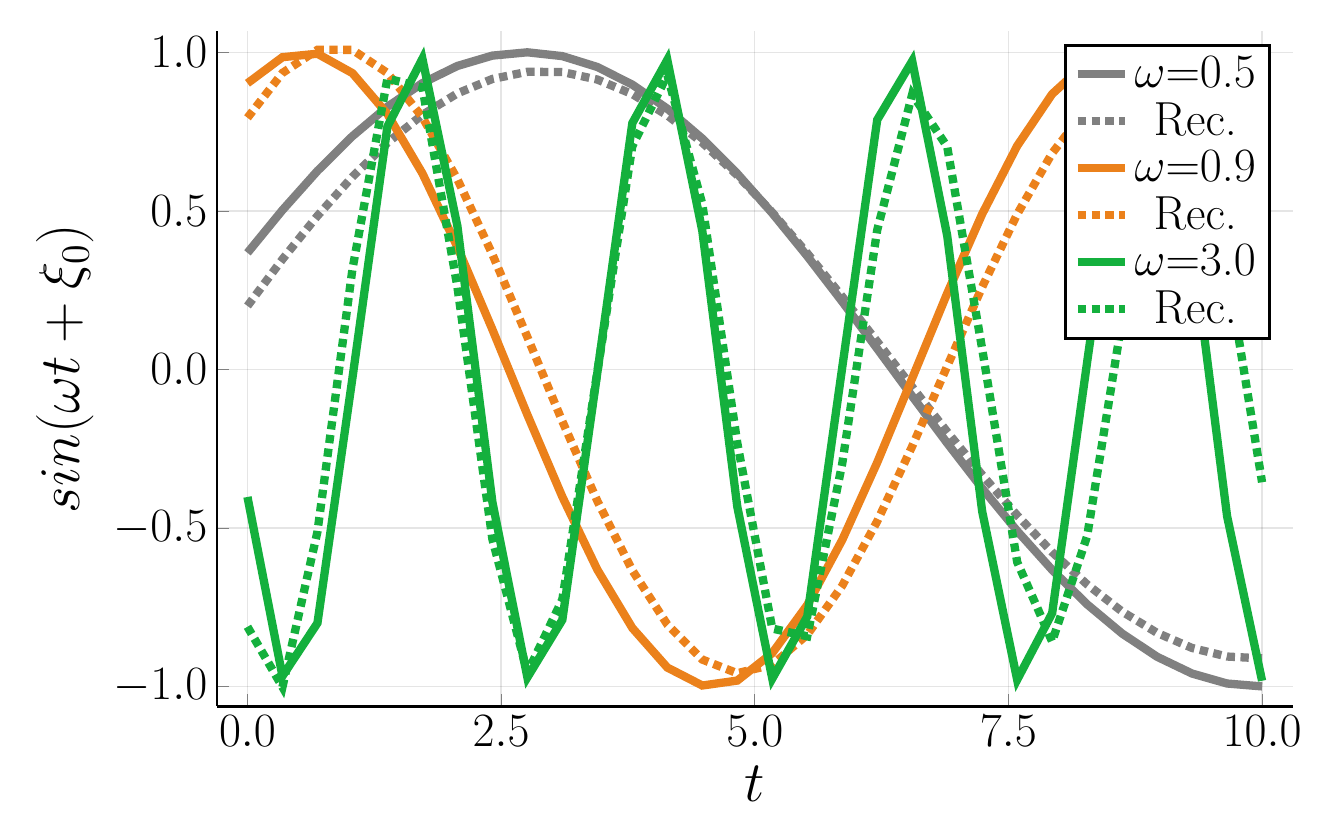
\begin{tikzpicture}[]
\begin{axis}[height = {101.6mm}, ylabel = {$\text{sin}(\omega t + \xi_0)$}, xmin = {-0.3}, xmax = {10.3}, ymax = {1.0681994700431823}, xlabel = {$t$}, unbounded coords=jump,scaled x ticks = false,xlabel style = {font = {\fontsize{22 pt}{28.6 pt}\selectfont}, color = {rgb,1:red,0.00000000;green,0.00000000;blue,0.00000000}, draw opacity = 1.0, rotate = 0.0},xmajorgrids = true,xtick = {0.0,2.5,5.0,7.5,10.0},xticklabels = {$0.0$,$2.5$,$5.0$,$7.5$,$10.0$},xtick align = inside,xticklabel style = {font = {\fontsize{16 pt}{20.8 pt}\selectfont}, color = {rgb,1:red,0.00000000;green,0.00000000;blue,0.00000000}, draw opacity = 1.0, rotate = 0.0},x grid style = {color = {rgb,1:red,0.00000000;green,0.00000000;blue,0.00000000},
draw opacity = 0.1,
line width = 0.5,
solid},axis x line* = left,x axis line style = {color = {rgb,1:red,0.00000000;green,0.00000000;blue,0.00000000},
draw opacity = 1.0,
line width = 1,
solid},scaled y ticks = false,ylabel style = {font = {\fontsize{22 pt}{28.6 pt}\selectfont}, color = {rgb,1:red,0.00000000;green,0.00000000;blue,0.00000000}, draw opacity = 1.0, rotate = 0.0},ymajorgrids = true,ytick = {-1.0,-0.5,0.0,0.5,1.0},yticklabels = {$-1.0$,$-0.5$,$0.0$,$0.5$,$1.0$},ytick align = inside,yticklabel style = {font = {\fontsize{16 pt}{20.8 pt}\selectfont}, color = {rgb,1:red,0.00000000;green,0.00000000;blue,0.00000000}, draw opacity = 1.0, rotate = 0.0},y grid style = {color = {rgb,1:red,0.00000000;green,0.00000000;blue,0.00000000},
draw opacity = 0.1,
line width = 0.5,
solid},axis y line* = left,y axis line style = {color = {rgb,1:red,0.00000000;green,0.00000000;blue,0.00000000},
draw opacity = 1.0,
line width = 1,
solid},    xshift = 0.0mm,
    yshift = 0.0mm,
    axis background/.style={fill={rgb,1:red,1.00000000;green,1.00000000;blue,1.00000000}}
,legend style = {color = {rgb,1:red,0.00000000;green,0.00000000;blue,0.00000000},
draw opacity = 1.0,
line width = 1,
solid,fill = {rgb,1:red,1.00000000;green,1.00000000;blue,1.00000000},font = {\fontsize{16 pt}{20.8 pt}\selectfont}},colorbar style={title=}, ymin = {-1.062116458415985}, width = {152.4mm}]\addplot+ [color = {rgb,1:red,0.50196078;green,0.50196078;blue,0.50196078},
draw opacity = 1.0,
line width = 3,
solid,mark = none,
mark size = 2.0,
mark options = {
    color = {rgb,1:red,0.00000000;green,0.00000000;blue,0.00000000}, draw opacity = 1.0,
    fill = {rgb,1:red,0.50196078;green,0.50196078;blue,0.50196078}, fill opacity = 1.0,
    line width = 1,
    rotate = 0,
    solid
}]coordinates {
(0.0, 0.36746644973754883)
(0.3448275862068966, 0.5023231506347656)
(0.6896551724137931, 0.6258987784385681)
(1.0344827586206897, 0.7354180216789246)
(1.3793103448275863, 0.828421413898468)
(1.7241379310344827, 0.9028202295303345)
(2.0689655172413794, 0.9569436311721802)
(2.413793103448276, 0.9895761609077454)
(2.7586206896551726, 0.9999849200248718)
(3.103448275862069, 0.9879361987113953)
(3.4482758620689653, 0.953700602054596)
(3.793103448275862, 0.8980468511581421)
(4.137931034482759, 0.8222249746322632)
(4.482758620689655, 0.7279376983642578)
(4.827586206896552, 0.6173024773597717)
(5.172413793103448, 0.4928039610385895)
(5.517241379310345, 0.35723814368247986)
(5.862068965517241, 0.21364955604076385)
(6.206896551724138, 0.06526283174753189)
(6.551724137931035, -0.08458954095840454)
(6.896551724137931, -0.2325422167778015)
(7.241379310344827, -0.3752725124359131)
(7.586206896551724, -0.5095749497413635)
(7.931034482758621, -0.6324334740638733)
(8.275862068965518, -0.7410889267921448)
(8.620689655172415, -0.8331010937690735)
(8.96551724137931, -0.9064036011695862)
(9.310344827586206, -0.9593502283096313)
(9.655172413793103, -0.9907519221305847)
(10.0, -0.9999035000801086)
};
\addlegendentry{$\omega$=0.5}
\addplot+ [color = {rgb,1:red,0.50196078;green,0.50196078;blue,0.50196078},
draw opacity = 1.0,
line width = 3,
dotted,mark = none,
mark size = 2.0,
mark options = {
    color = {rgb,1:red,0.00000000;green,0.00000000;blue,0.00000000}, draw opacity = 1.0,
    fill = {rgb,1:red,0.50196078;green,0.50196078;blue,0.50196078}, fill opacity = 1.0,
    line width = 1,
    rotate = 0,
    solid
}]coordinates {
(0.0, 0.2000093162059784)
(0.3448275862068966, 0.3473007082939148)
(0.6896551724137931, 0.484201580286026)
(1.0344827586206897, 0.6075544357299805)
(1.3793103448275863, 0.7145543098449707)
(1.7241379310344827, 0.8028115034103394)
(2.0689655172413794, 0.8704048991203308)
(2.413793103448276, 0.9159235954284668)
(2.7586206896551726, 0.9384945034980774)
(3.103448275862069, 0.9377992749214172)
(3.4482758620689653, 0.9140751957893372)
(3.793103448275862, 0.8681065440177917)
(4.137931034482759, 0.8011984825134277)
(4.482758620689655, 0.7151414155960083)
(4.827586206896552, 0.6121646761894226)
(5.172413793103448, 0.49487993121147156)
(5.517241379310345, 0.36621129512786865)
(5.862068965517241, 0.22933004796504974)
(6.206896551724138, 0.08757191896438599)
(6.551724137931035, -0.05564840883016586)
(6.896551724137931, -0.19690442085266113)
(7.241379310344827, -0.3328574001789093)
(7.586206896551724, -0.4603240489959717)
(7.931034482758621, -0.5763473510742188)
(8.275862068965518, -0.678280770778656)
(8.620689655172415, -0.7638316750526428)
(8.96551724137931, -0.8311143517494202)
(9.310344827586206, -0.8787083625793457)
(9.655172413793103, -0.9056657552719116)
(10.0, -0.9115384817123413)
};
\addlegendentry{Rec.}
\addplot+ [color = {rgb,1:red,0.92156863;green,0.50588235;blue,0.10588235},
draw opacity = 1.0,
line width = 3,
solid,mark = none,
mark size = 2.0,
mark options = {
    color = {rgb,1:red,0.00000000;green,0.00000000;blue,0.00000000}, draw opacity = 1.0,
    fill = {rgb,1:red,0.92156863;green,0.50588235;blue,0.10588235}, fill opacity = 1.0,
    line width = 1,
    rotate = 0,
    solid
}]coordinates {
(0.0, 0.9023802876472473)
(0.3448275862068966, 0.9846332669258118)
(0.6896551724137931, 0.995541512966156)
(1.0344827586206897, 0.9343145489692688)
(1.3793103448275863, 0.805388867855072)
(1.7241379310344827, 0.6181061267852783)
(2.0689655172413794, 0.38603654503822327)
(2.413793103448276, 0.1259954273700714)
(2.7586206896551726, -0.14317508041858673)
(3.103448275862069, -0.40197136998176575)
(3.4482758620689653, -0.6316415667533875)
(3.793103448275862, -0.8155441284179688)
(4.137931034482759, -0.9403538107872009)
(4.482758620689655, -0.9970271587371826)
(4.827586206896552, -0.9814577102661133)
(5.172413793103448, -0.894773542881012)
(5.517241379310345, -0.7432557344436646)
(5.862068965517241, -0.5378829836845398)
(6.206896551724138, -0.29353615641593933)
(6.551724137931035, -0.02792022004723549)
(6.896551724137931, 0.2397187501192093)
(7.241379310344827, 0.48998814821243286)
(7.586206896551724, 0.7047538757324219)
(7.931034482758621, 0.8684543967247009)
(8.275862068965518, 0.9692282676696777)
(8.620689655172415, 0.9997736215591431)
(8.96551724137931, 0.9578770995140076)
(9.310344827586206, 0.846574604511261)
(9.655172413793103, 0.6739307641983032)
(10.0, 0.45245516300201416)
};
\addlegendentry{$\omega$=0.9}
\addplot+ [color = {rgb,1:red,0.92156863;green,0.50588235;blue,0.10588235},
draw opacity = 1.0,
line width = 3,
dotted,mark = none,
mark size = 2.0,
mark options = {
    color = {rgb,1:red,0.00000000;green,0.00000000;blue,0.00000000}, draw opacity = 1.0,
    fill = {rgb,1:red,0.92156863;green,0.50588235;blue,0.10588235}, fill opacity = 1.0,
    line width = 1,
    rotate = 0,
    solid
}]coordinates {
(0.0, 0.7935009002685547)
(0.3448275862068966, 0.9349510669708252)
(0.6896551724137931, 1.007907509803772)
(1.0344827586206897, 1.007662057876587)
(1.3793103448275863, 0.9348446130752563)
(1.7241379310344827, 0.795332670211792)
(2.0689655172413794, 0.5997823476791382)
(2.413793103448276, 0.36281663179397583)
(2.7586206896551726, 0.10193541646003723)
(3.103448275862069, -0.16377997398376465)
(3.4482758620689653, -0.4150541126728058)
(3.793103448275862, -0.633815348148346)
(4.137931034482759, -0.8045057058334351)
(4.482758620689655, -0.915166974067688)
(4.827586206896552, -0.9582892060279846)
(5.172413793103448, -0.9313194155693054)
(5.517241379310345, -0.8367851972579956)
(5.862068965517241, -0.6821047067642212)
(6.206896551724138, -0.4789621829986572)
(6.551724137931035, -0.24248191714286804)
(6.896551724137931, 0.009961336851119995)
(7.241379310344827, 0.2599397301673889)
(7.586206896551724, 0.48940154910087585)
(7.931034482758621, 0.6818888187408447)
(8.275862068965518, 0.8238027691841125)
(8.620689655172415, 0.9052634239196777)
(8.96551724137931, 0.9209101796150208)
(9.310344827586206, 0.8701364994049072)
(9.655172413793103, 0.7571859359741211)
(10.0, 0.5907527208328247)
};
\addlegendentry{Rec.}
\addplot+ [color = {rgb,1:red,0.07843137;green,0.69019608;blue,0.23921569},
draw opacity = 1.0,
line width = 3,
solid,mark = none,
mark size = 2.0,
mark options = {
    color = {rgb,1:red,0.00000000;green,0.00000000;blue,0.00000000}, draw opacity = 1.0,
    fill = {rgb,1:red,0.07843137;green,0.69019608;blue,0.23921569}, fill opacity = 1.0,
    line width = 1,
    rotate = 0,
    solid
}]coordinates {
(0.0, -0.4023912847042084)
(0.3448275862068966, -0.9672409892082214)
(0.6896551724137931, -0.8001019954681396)
(1.0344827586206897, -0.02746175043284893)
(1.3793103448275863, 0.7659609913825989)
(1.7241379310344827, 0.9797196984291077)
(2.0689655172413794, 0.45204609632492065)
(2.413793103448276, -0.417726993560791)
(2.7586206896551726, -0.9713726043701172)
(3.103448275862069, -0.7899028062820435)
(3.4482758620689653, -0.01065030973404646)
(3.793103448275862, 0.7766621708869934)
(4.137931034482759, 0.9762121438980103)
(4.482758620689655, 0.4369843006134033)
(4.827586206896552, -0.4329445958137512)
(5.172413793103448, -0.9752296209335327)
(5.517241379310345, -0.7794803380966187)
(5.862068965517241, 0.006164142861962318)
(6.206896551724138, 0.7871437072753906)
(6.551724137931035, 0.9724286198616028)
(6.896551724137931, 0.4217989444732666)
(7.241379310344827, -0.4480397701263428)
(7.586206896551724, -0.9788109064102173)
(7.931034482758621, -0.7688374519348145)
(8.275862068965518, 0.02297685295343399)
(8.620689655172415, 0.7974027395248413)
(8.96551724137931, 0.9683701395988464)
(9.310344827586206, 0.4064943194389343)
(9.655172413793103, -0.463008314371109)
(10.0, -0.9821154475212097)
};
\addlegendentry{$\omega$=3.0}
\addplot+ [color = {rgb,1:red,0.07843137;green,0.69019608;blue,0.23921569},
draw opacity = 1.0,
line width = 3,
dotted,mark = none,
mark size = 2.0,
mark options = {
    color = {rgb,1:red,0.00000000;green,0.00000000;blue,0.00000000}, draw opacity = 1.0,
    fill = {rgb,1:red,0.07843137;green,0.69019608;blue,0.23921569}, fill opacity = 1.0,
    line width = 1,
    rotate = 0,
    solid
}]coordinates {
(0.0, -0.8117820620536804)
(0.3448275862068966, -1.0018244981765747)
(0.6896551724137931, -0.5120609998703003)
(1.0344827586206897, 0.3159843683242798)
(1.3793103448275863, 0.9174131155014038)
(1.7241379310344827, 0.889211118221283)
(2.0689655172413794, 0.26015156507492065)
(2.413793103448276, -0.5353266596794128)
(2.7586206896551726, -0.9569792151451111)
(3.103448275862069, -0.7255999445915222)
(3.4482758620689653, -0.0076377540826797485)
(3.793103448275862, 0.7041017413139343)
(4.137931034482759, 0.9286616444587708)
(4.482758620689655, 0.5217524766921997)
(4.827586206896552, -0.23184382915496826)
(5.172413793103448, -0.8174175024032593)
(5.517241379310345, -0.8417914509773254)
(5.862068965517241, -0.29713040590286255)
(6.206896551724138, 0.43963390588760376)
(6.551724137931035, 0.8675405979156494)
(6.896551724137931, 0.7021247744560242)
(7.241379310344827, 0.06435912847518921)
(7.586206896551724, -0.607422947883606)
(7.931034482758621, -0.8586357831954956)
(8.275862068965518, -0.5259531140327454)
(8.620689655172415, 0.1567382514476776)
(8.96551724137931, 0.7225946187973022)
(9.310344827586206, 0.7909285426139832)
(9.655172413793103, 0.32324549555778503)
(10.0, -0.35607677698135376)
};
\addlegendentry{Rec.}
\end{axis}

\end{tikzpicture}
}
\end{frame}

\begin{frame}{Results - Latent space}
  \resizebox{!}{.28\linewidth}{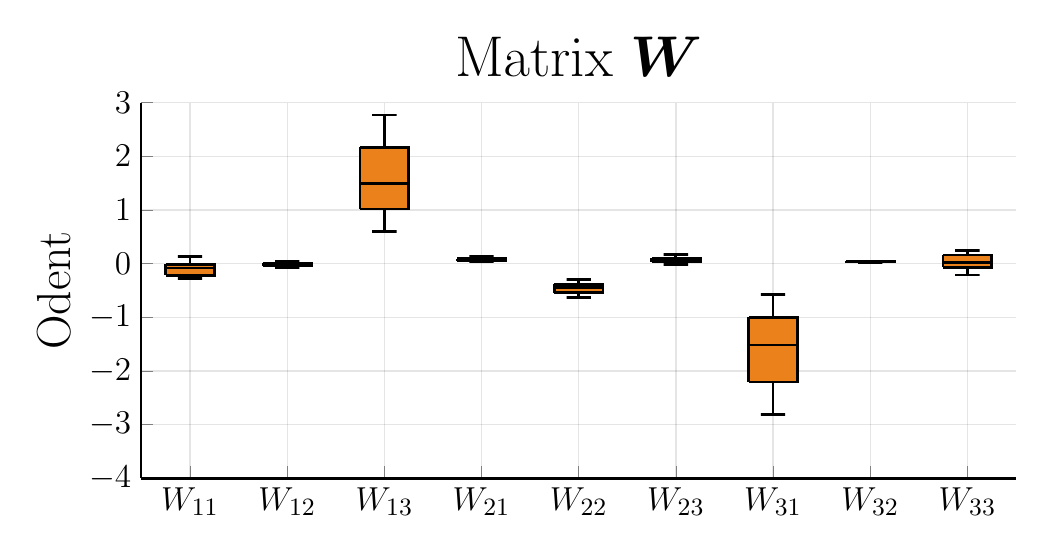
\begin{tikzpicture}[]
\begin{axis}[height = {63.5mm}, ylabel = {Odent}, title = {Matrix $\bm W$}, xmin = {-0.0050000000000000044}, xmax = {9.005}, ymax = {3}, xlabel = {}, unbounded coords=jump,scaled x ticks = false,xlabel style = {font = {\fontsize{18 pt}{23.400000000000002 pt}\selectfont}, color = {rgb,1:red,0.00000000;green,0.00000000;blue,0.00000000}, draw opacity = 1.0, rotate = 0.0},xmajorgrids = true,xtick = {0.5,1.5,2.5,3.5,4.5,5.5,6.5,7.5,8.5},xticklabels = {$W_{11}$,$W_{12}$,$W_{13}$,$W_{21}$,$W_{22}$,$W_{23}$,$W_{31}$,$W_{32}$,$W_{33}$},xtick align = inside,xticklabel style = {font = {\fontsize{13 pt}{16.900000000000002 pt}\selectfont}, color = {rgb,1:red,0.00000000;green,0.00000000;blue,0.00000000}, draw opacity = 1.0, rotate = 0.0},x grid style = {color = {rgb,1:red,0.00000000;green,0.00000000;blue,0.00000000},
draw opacity = 0.1,
line width = 0.5,
solid},axis x line* = left,x axis line style = {color = {rgb,1:red,0.00000000;green,0.00000000;blue,0.00000000},
draw opacity = 1.0,
line width = 1,
solid},scaled y ticks = false,ylabel style = {font = {\fontsize{18 pt}{23.400000000000002 pt}\selectfont}, color = {rgb,1:red,0.00000000;green,0.00000000;blue,0.00000000}, draw opacity = 1.0, rotate = 0.0},ymajorgrids = true,ytick = {-4.0,-3.0,-2.0,-1.0,0.0,1.0,2.0,3.0},yticklabels = {$-4$,$-3$,$-2$,$-1$,$0$,$1$,$2$,$3$},ytick align = inside,yticklabel style = {font = {\fontsize{13 pt}{16.900000000000002 pt}\selectfont}, color = {rgb,1:red,0.00000000;green,0.00000000;blue,0.00000000}, draw opacity = 1.0, rotate = 0.0},y grid style = {color = {rgb,1:red,0.00000000;green,0.00000000;blue,0.00000000},
draw opacity = 0.1,
line width = 0.5,
solid},axis y line* = left,y axis line style = {color = {rgb,1:red,0.00000000;green,0.00000000;blue,0.00000000},
draw opacity = 1.0,
line width = 1,
solid},    xshift = 0.0mm,
    yshift = 0.0mm,
    axis background/.style={fill={rgb,1:red,1.00000000;green,1.00000000;blue,1.00000000}}
,title style = {font = {\fontsize{22 pt}{28.6 pt}\selectfont}, color = {rgb,1:red,0.00000000;green,0.00000000;blue,0.00000000}, draw opacity = 1.0, rotate = 0.0},legend style = {color = {rgb,1:red,0.00000000;green,0.00000000;blue,0.00000000},
draw opacity = 1.0,
line width = 1,
solid,fill = {rgb,1:red,1.00000000;green,1.00000000;blue,1.00000000},font = {\fontsize{13 pt}{16.900000000000002 pt}\selectfont}},colorbar style={title=}, ymin = {-4}, width = {127.0mm}]\addplot+ [color = {rgb,1:red,0.00000000;green,0.00000000;blue,0.00000000},
draw opacity = 1.0,
line width = 1,
solid,mark = none,
mark size = 2.0,
mark options = {
    color = {rgb,1:red,0.00000000;green,0.00000000;blue,0.00000000}, draw opacity = 1.0,
    fill = {rgb,1:red,0.92156863;green,0.50588235;blue,0.10588235}, fill opacity = 1.0,
    line width = 1,
    rotate = 0,
    solid
},fill = {rgb,1:red,0.92156863;green,0.50588235;blue,0.10588235}, fill opacity=1.0,forget plot]coordinates {
(0.5, -0.28068220615386963)
(0.375, -0.28068220615386963)
(0.625, -0.28068220615386963)
(0.5, -0.28068220615386963)
(0.5, -0.21647277101874352)
};
\addplot+ [color = {rgb,1:red,0.00000000;green,0.00000000;blue,0.00000000},
draw opacity = 1.0,
line width = 1,
solid,mark = none,
mark size = 2.0,
mark options = {
    color = {rgb,1:red,0.00000000;green,0.00000000;blue,0.00000000}, draw opacity = 1.0,
    fill = {rgb,1:red,0.92156863;green,0.50588235;blue,0.10588235}, fill opacity = 1.0,
    line width = 1,
    rotate = 0,
    solid
},fill = {rgb,1:red,0.92156863;green,0.50588235;blue,0.10588235}, fill opacity=1.0,forget plot]coordinates {
(0.25, -0.21647277101874352)
(0.25, -0.08380848169326782)
(0.75, -0.08380848169326782)
(0.75, -0.21647277101874352)
(0.25, -0.21647277101874352)
};
\addplot+ [color = {rgb,1:red,0.00000000;green,0.00000000;blue,0.00000000},
draw opacity = 1.0,
line width = 1,
solid,mark = none,
mark size = 2.0,
mark options = {
    color = {rgb,1:red,0.00000000;green,0.00000000;blue,0.00000000}, draw opacity = 1.0,
    fill = {rgb,1:red,0.92156863;green,0.50588235;blue,0.10588235}, fill opacity = 1.0,
    line width = 1,
    rotate = 0,
    solid
},fill = {rgb,1:red,0.92156863;green,0.50588235;blue,0.10588235}, fill opacity=1.0,forget plot]coordinates {
(0.25, -0.011269278824329376)
(0.25, -0.08380848169326782)
(0.75, -0.08380848169326782)
(0.75, -0.011269278824329376)
(0.25, -0.011269278824329376)
};
\addplot+ [color = {rgb,1:red,0.00000000;green,0.00000000;blue,0.00000000},
draw opacity = 1.0,
line width = 1,
solid,mark = none,
mark size = 2.0,
mark options = {
    color = {rgb,1:red,0.00000000;green,0.00000000;blue,0.00000000}, draw opacity = 1.0,
    fill = {rgb,1:red,0.92156863;green,0.50588235;blue,0.10588235}, fill opacity = 1.0,
    line width = 1,
    rotate = 0,
    solid
},fill = {rgb,1:red,0.92156863;green,0.50588235;blue,0.10588235}, fill opacity=1.0,forget plot]coordinates {
(0.5, 0.1312718391418457)
(0.375, 0.1312718391418457)
(0.625, 0.1312718391418457)
(0.5, 0.1312718391418457)
(0.5, -0.011269278824329376)
};
\addplot+ [color = {rgb,1:red,0.00000000;green,0.00000000;blue,0.00000000},
draw opacity = 1.0,
line width = 1,
solid,mark = none,
mark size = 2.0,
mark options = {
    color = {rgb,1:red,0.00000000;green,0.00000000;blue,0.00000000}, draw opacity = 1.0,
    fill = {rgb,1:red,0.92156863;green,0.50588235;blue,0.10588235}, fill opacity = 1.0,
    line width = 1,
    rotate = 0,
    solid
},fill = {rgb,1:red,0.92156863;green,0.50588235;blue,0.10588235}, fill opacity=1.0,forget plot]coordinates {
(1.5, -0.08050356060266495)
(1.375, -0.08050356060266495)
(1.625, -0.08050356060266495)
(1.5, -0.08050356060266495)
(1.5, -0.035347397439181805)
};
\addplot+ [color = {rgb,1:red,0.00000000;green,0.00000000;blue,0.00000000},
draw opacity = 1.0,
line width = 1,
solid,mark = none,
mark size = 2.0,
mark options = {
    color = {rgb,1:red,0.00000000;green,0.00000000;blue,0.00000000}, draw opacity = 1.0,
    fill = {rgb,1:red,0.92156863;green,0.50588235;blue,0.10588235}, fill opacity = 1.0,
    line width = 1,
    rotate = 0,
    solid
},fill = {rgb,1:red,0.92156863;green,0.50588235;blue,0.10588235}, fill opacity=1.0,forget plot]coordinates {
(1.25, -0.035347397439181805)
(1.25, -0.015371293295174837)
(1.75, -0.015371293295174837)
(1.75, -0.035347397439181805)
(1.25, -0.035347397439181805)
};
\addplot+ [color = {rgb,1:red,0.00000000;green,0.00000000;blue,0.00000000},
draw opacity = 1.0,
line width = 1,
solid,mark = none,
mark size = 2.0,
mark options = {
    color = {rgb,1:red,0.00000000;green,0.00000000;blue,0.00000000}, draw opacity = 1.0,
    fill = {rgb,1:red,0.92156863;green,0.50588235;blue,0.10588235}, fill opacity = 1.0,
    line width = 1,
    rotate = 0,
    solid
},fill = {rgb,1:red,0.92156863;green,0.50588235;blue,0.10588235}, fill opacity=1.0,forget plot]coordinates {
(1.25, 0.006936707533895969)
(1.25, -0.015371293295174837)
(1.75, -0.015371293295174837)
(1.75, 0.006936707533895969)
(1.25, 0.006936707533895969)
};
\addplot+ [color = {rgb,1:red,0.00000000;green,0.00000000;blue,0.00000000},
draw opacity = 1.0,
line width = 1,
solid,mark = none,
mark size = 2.0,
mark options = {
    color = {rgb,1:red,0.00000000;green,0.00000000;blue,0.00000000}, draw opacity = 1.0,
    fill = {rgb,1:red,0.92156863;green,0.50588235;blue,0.10588235}, fill opacity = 1.0,
    line width = 1,
    rotate = 0,
    solid
},fill = {rgb,1:red,0.92156863;green,0.50588235;blue,0.10588235}, fill opacity=1.0,forget plot]coordinates {
(1.5, 0.043295323848724365)
(1.375, 0.043295323848724365)
(1.625, 0.043295323848724365)
(1.5, 0.043295323848724365)
(1.5, 0.006936707533895969)
};
\addplot+ [color = {rgb,1:red,0.00000000;green,0.00000000;blue,0.00000000},
draw opacity = 1.0,
line width = 1,
solid,mark = none,
mark size = 2.0,
mark options = {
    color = {rgb,1:red,0.00000000;green,0.00000000;blue,0.00000000}, draw opacity = 1.0,
    fill = {rgb,1:red,0.92156863;green,0.50588235;blue,0.10588235}, fill opacity = 1.0,
    line width = 1,
    rotate = 0,
    solid
},fill = {rgb,1:red,0.92156863;green,0.50588235;blue,0.10588235}, fill opacity=1.0,forget plot]coordinates {
(2.5, 0.5995415449142456)
(2.375, 0.5995415449142456)
(2.625, 0.5995415449142456)
(2.5, 0.5995415449142456)
(2.5, 1.0167028605937958)
};
\addplot+ [color = {rgb,1:red,0.00000000;green,0.00000000;blue,0.00000000},
draw opacity = 1.0,
line width = 1,
solid,mark = none,
mark size = 2.0,
mark options = {
    color = {rgb,1:red,0.00000000;green,0.00000000;blue,0.00000000}, draw opacity = 1.0,
    fill = {rgb,1:red,0.92156863;green,0.50588235;blue,0.10588235}, fill opacity = 1.0,
    line width = 1,
    rotate = 0,
    solid
},fill = {rgb,1:red,0.92156863;green,0.50588235;blue,0.10588235}, fill opacity=1.0,forget plot]coordinates {
(2.25, 1.0167028605937958)
(2.25, 1.4863724112510681)
(2.75, 1.4863724112510681)
(2.75, 1.0167028605937958)
(2.25, 1.0167028605937958)
};
\addplot+ [color = {rgb,1:red,0.00000000;green,0.00000000;blue,0.00000000},
draw opacity = 1.0,
line width = 1,
solid,mark = none,
mark size = 2.0,
mark options = {
    color = {rgb,1:red,0.00000000;green,0.00000000;blue,0.00000000}, draw opacity = 1.0,
    fill = {rgb,1:red,0.92156863;green,0.50588235;blue,0.10588235}, fill opacity = 1.0,
    line width = 1,
    rotate = 0,
    solid
},fill = {rgb,1:red,0.92156863;green,0.50588235;blue,0.10588235}, fill opacity=1.0,forget plot]coordinates {
(2.25, 2.1655468344688416)
(2.25, 1.4863724112510681)
(2.75, 1.4863724112510681)
(2.75, 2.1655468344688416)
(2.25, 2.1655468344688416)
};
\addplot+ [color = {rgb,1:red,0.00000000;green,0.00000000;blue,0.00000000},
draw opacity = 1.0,
line width = 1,
solid,mark = none,
mark size = 2.0,
mark options = {
    color = {rgb,1:red,0.00000000;green,0.00000000;blue,0.00000000}, draw opacity = 1.0,
    fill = {rgb,1:red,0.92156863;green,0.50588235;blue,0.10588235}, fill opacity = 1.0,
    line width = 1,
    rotate = 0,
    solid
},fill = {rgb,1:red,0.92156863;green,0.50588235;blue,0.10588235}, fill opacity=1.0,forget plot]coordinates {
(2.5, 2.770195484161377)
(2.375, 2.770195484161377)
(2.625, 2.770195484161377)
(2.5, 2.770195484161377)
(2.5, 2.1655468344688416)
};
\addplot+ [color = {rgb,1:red,0.00000000;green,0.00000000;blue,0.00000000},
draw opacity = 1.0,
line width = 1,
solid,mark = none,
mark size = 2.0,
mark options = {
    color = {rgb,1:red,0.00000000;green,0.00000000;blue,0.00000000}, draw opacity = 1.0,
    fill = {rgb,1:red,0.92156863;green,0.50588235;blue,0.10588235}, fill opacity = 1.0,
    line width = 1,
    rotate = 0,
    solid
},fill = {rgb,1:red,0.92156863;green,0.50588235;blue,0.10588235}, fill opacity=1.0,forget plot]coordinates {
(3.5, 0.029579564929008484)
(3.375, 0.029579564929008484)
(3.625, 0.029579564929008484)
(3.5, 0.029579564929008484)
(3.5, 0.05103161372244358)
};
\addplot+ [color = {rgb,1:red,0.00000000;green,0.00000000;blue,0.00000000},
draw opacity = 1.0,
line width = 1,
solid,mark = none,
mark size = 2.0,
mark options = {
    color = {rgb,1:red,0.00000000;green,0.00000000;blue,0.00000000}, draw opacity = 1.0,
    fill = {rgb,1:red,0.92156863;green,0.50588235;blue,0.10588235}, fill opacity = 1.0,
    line width = 1,
    rotate = 0,
    solid
},fill = {rgb,1:red,0.92156863;green,0.50588235;blue,0.10588235}, fill opacity=1.0,forget plot]coordinates {
(3.25, 0.05103161372244358)
(3.25, 0.06557240709662437)
(3.75, 0.06557240709662437)
(3.75, 0.05103161372244358)
(3.25, 0.05103161372244358)
};
\addplot+ [color = {rgb,1:red,0.00000000;green,0.00000000;blue,0.00000000},
draw opacity = 1.0,
line width = 1,
solid,mark = none,
mark size = 2.0,
mark options = {
    color = {rgb,1:red,0.00000000;green,0.00000000;blue,0.00000000}, draw opacity = 1.0,
    fill = {rgb,1:red,0.92156863;green,0.50588235;blue,0.10588235}, fill opacity = 1.0,
    line width = 1,
    rotate = 0,
    solid
},fill = {rgb,1:red,0.92156863;green,0.50588235;blue,0.10588235}, fill opacity=1.0,forget plot]coordinates {
(3.25, 0.08917277306318283)
(3.25, 0.06557240709662437)
(3.75, 0.06557240709662437)
(3.75, 0.08917277306318283)
(3.25, 0.08917277306318283)
};
\addplot+ [color = {rgb,1:red,0.00000000;green,0.00000000;blue,0.00000000},
draw opacity = 1.0,
line width = 1,
solid,mark = none,
mark size = 2.0,
mark options = {
    color = {rgb,1:red,0.00000000;green,0.00000000;blue,0.00000000}, draw opacity = 1.0,
    fill = {rgb,1:red,0.92156863;green,0.50588235;blue,0.10588235}, fill opacity = 1.0,
    line width = 1,
    rotate = 0,
    solid
},fill = {rgb,1:red,0.92156863;green,0.50588235;blue,0.10588235}, fill opacity=1.0,forget plot]coordinates {
(3.5, 0.12536239624023438)
(3.375, 0.12536239624023438)
(3.625, 0.12536239624023438)
(3.5, 0.12536239624023438)
(3.5, 0.08917277306318283)
};
\addplot+ [color = {rgb,1:red,0.00000000;green,0.00000000;blue,0.00000000},
draw opacity = 1.0,
line width = 1,
solid,mark = none,
mark size = 2.0,
mark options = {
    color = {rgb,1:red,0.00000000;green,0.00000000;blue,0.00000000}, draw opacity = 1.0,
    fill = {rgb,1:red,0.92156863;green,0.50588235;blue,0.10588235}, fill opacity = 1.0,
    line width = 1,
    rotate = 0,
    solid
},fill = {rgb,1:red,0.92156863;green,0.50588235;blue,0.10588235}, fill opacity=1.0,forget plot]coordinates {
(4.5, -0.6291252374649048)
(4.375, -0.6291252374649048)
(4.625, -0.6291252374649048)
(4.5, -0.6291252374649048)
(4.5, -0.541555717587471)
};
\addplot+ [color = {rgb,1:red,0.00000000;green,0.00000000;blue,0.00000000},
draw opacity = 1.0,
line width = 1,
solid,mark = none,
mark size = 2.0,
mark options = {
    color = {rgb,1:red,0.00000000;green,0.00000000;blue,0.00000000}, draw opacity = 1.0,
    fill = {rgb,1:red,0.92156863;green,0.50588235;blue,0.10588235}, fill opacity = 1.0,
    line width = 1,
    rotate = 0,
    solid
},fill = {rgb,1:red,0.92156863;green,0.50588235;blue,0.10588235}, fill opacity=1.0,forget plot]coordinates {
(4.25, -0.541555717587471)
(4.25, -0.44207364320755005)
(4.75, -0.44207364320755005)
(4.75, -0.541555717587471)
(4.25, -0.541555717587471)
};
\addplot+ [color = {rgb,1:red,0.00000000;green,0.00000000;blue,0.00000000},
draw opacity = 1.0,
line width = 1,
solid,mark = none,
mark size = 2.0,
mark options = {
    color = {rgb,1:red,0.00000000;green,0.00000000;blue,0.00000000}, draw opacity = 1.0,
    fill = {rgb,1:red,0.92156863;green,0.50588235;blue,0.10588235}, fill opacity = 1.0,
    line width = 1,
    rotate = 0,
    solid
},fill = {rgb,1:red,0.92156863;green,0.50588235;blue,0.10588235}, fill opacity=1.0,forget plot]coordinates {
(4.25, -0.3845475763082504)
(4.25, -0.44207364320755005)
(4.75, -0.44207364320755005)
(4.75, -0.3845475763082504)
(4.25, -0.3845475763082504)
};
\addplot+ [color = {rgb,1:red,0.00000000;green,0.00000000;blue,0.00000000},
draw opacity = 1.0,
line width = 1,
solid,mark = none,
mark size = 2.0,
mark options = {
    color = {rgb,1:red,0.00000000;green,0.00000000;blue,0.00000000}, draw opacity = 1.0,
    fill = {rgb,1:red,0.92156863;green,0.50588235;blue,0.10588235}, fill opacity = 1.0,
    line width = 1,
    rotate = 0,
    solid
},fill = {rgb,1:red,0.92156863;green,0.50588235;blue,0.10588235}, fill opacity=1.0,forget plot]coordinates {
(4.5, -0.29447871446609497)
(4.375, -0.29447871446609497)
(4.625, -0.29447871446609497)
(4.5, -0.29447871446609497)
(4.5, -0.3845475763082504)
};
\addplot+ [color = {rgb,1:red,0.00000000;green,0.00000000;blue,0.00000000},
draw opacity = 1.0,
line width = 1,
solid,mark = none,
mark size = 2.0,
mark options = {
    color = {rgb,1:red,0.00000000;green,0.00000000;blue,0.00000000}, draw opacity = 1.0,
    fill = {rgb,1:red,0.92156863;green,0.50588235;blue,0.10588235}, fill opacity = 1.0,
    line width = 1,
    rotate = 0,
    solid
},fill = {rgb,1:red,0.92156863;green,0.50588235;blue,0.10588235}, fill opacity=1.0,forget plot]coordinates {
(5.5, -0.011228802613914013)
(5.375, -0.011228802613914013)
(5.625, -0.011228802613914013)
(5.5, -0.011228802613914013)
(5.5, 0.03523004241287708)
};
\addplot+ [color = {rgb,1:red,0.00000000;green,0.00000000;blue,0.00000000},
draw opacity = 1.0,
line width = 1,
solid,mark = none,
mark size = 2.0,
mark options = {
    color = {rgb,1:red,0.00000000;green,0.00000000;blue,0.00000000}, draw opacity = 1.0,
    fill = {rgb,1:red,0.92156863;green,0.50588235;blue,0.10588235}, fill opacity = 1.0,
    line width = 1,
    rotate = 0,
    solid
},fill = {rgb,1:red,0.92156863;green,0.50588235;blue,0.10588235}, fill opacity=1.0,forget plot]coordinates {
(5.25, 0.03523004241287708)
(5.25, 0.07538121193647385)
(5.75, 0.07538121193647385)
(5.75, 0.03523004241287708)
(5.25, 0.03523004241287708)
};
\addplot+ [color = {rgb,1:red,0.00000000;green,0.00000000;blue,0.00000000},
draw opacity = 1.0,
line width = 1,
solid,mark = none,
mark size = 2.0,
mark options = {
    color = {rgb,1:red,0.00000000;green,0.00000000;blue,0.00000000}, draw opacity = 1.0,
    fill = {rgb,1:red,0.92156863;green,0.50588235;blue,0.10588235}, fill opacity = 1.0,
    line width = 1,
    rotate = 0,
    solid
},fill = {rgb,1:red,0.92156863;green,0.50588235;blue,0.10588235}, fill opacity=1.0,forget plot]coordinates {
(5.25, 0.08912588469684124)
(5.25, 0.07538121193647385)
(5.75, 0.07538121193647385)
(5.75, 0.08912588469684124)
(5.25, 0.08912588469684124)
};
\addplot+ [color = {rgb,1:red,0.00000000;green,0.00000000;blue,0.00000000},
draw opacity = 1.0,
line width = 1,
solid,mark = none,
mark size = 2.0,
mark options = {
    color = {rgb,1:red,0.00000000;green,0.00000000;blue,0.00000000}, draw opacity = 1.0,
    fill = {rgb,1:red,0.92156863;green,0.50588235;blue,0.10588235}, fill opacity = 1.0,
    line width = 1,
    rotate = 0,
    solid
},fill = {rgb,1:red,0.92156863;green,0.50588235;blue,0.10588235}, fill opacity=1.0,forget plot]coordinates {
(5.5, 0.1649191528558731)
(5.375, 0.1649191528558731)
(5.625, 0.1649191528558731)
(5.5, 0.1649191528558731)
(5.5, 0.08912588469684124)
};
\addplot+ [color = {rgb,1:red,0.00000000;green,0.00000000;blue,0.00000000},
draw opacity = 1.0,
line width = 1,
solid,mark = none,
mark size = 2.0,
mark options = {
    color = {rgb,1:red,0.00000000;green,0.00000000;blue,0.00000000}, draw opacity = 1.0,
    fill = {rgb,1:red,0.92156863;green,0.50588235;blue,0.10588235}, fill opacity = 1.0,
    line width = 1,
    rotate = 0,
    solid
},fill = {rgb,1:red,0.92156863;green,0.50588235;blue,0.10588235}, fill opacity=1.0,forget plot]coordinates {
(6.5, -2.8087313175201416)
(6.375, -2.8087313175201416)
(6.625, -2.8087313175201416)
(6.5, -2.8087313175201416)
(6.5, -2.2075082659721375)
};
\addplot+ [color = {rgb,1:red,0.00000000;green,0.00000000;blue,0.00000000},
draw opacity = 1.0,
line width = 1,
solid,mark = none,
mark size = 2.0,
mark options = {
    color = {rgb,1:red,0.00000000;green,0.00000000;blue,0.00000000}, draw opacity = 1.0,
    fill = {rgb,1:red,0.92156863;green,0.50588235;blue,0.10588235}, fill opacity = 1.0,
    line width = 1,
    rotate = 0,
    solid
},fill = {rgb,1:red,0.92156863;green,0.50588235;blue,0.10588235}, fill opacity=1.0,forget plot]coordinates {
(6.25, -2.2075082659721375)
(6.25, -1.51871258020401)
(6.75, -1.51871258020401)
(6.75, -2.2075082659721375)
(6.25, -2.2075082659721375)
};
\addplot+ [color = {rgb,1:red,0.00000000;green,0.00000000;blue,0.00000000},
draw opacity = 1.0,
line width = 1,
solid,mark = none,
mark size = 2.0,
mark options = {
    color = {rgb,1:red,0.00000000;green,0.00000000;blue,0.00000000}, draw opacity = 1.0,
    fill = {rgb,1:red,0.92156863;green,0.50588235;blue,0.10588235}, fill opacity = 1.0,
    line width = 1,
    rotate = 0,
    solid
},fill = {rgb,1:red,0.92156863;green,0.50588235;blue,0.10588235}, fill opacity=1.0,forget plot]coordinates {
(6.25, -1.0012929439544678)
(6.25, -1.51871258020401)
(6.75, -1.51871258020401)
(6.75, -1.0012929439544678)
(6.25, -1.0012929439544678)
};
\addplot+ [color = {rgb,1:red,0.00000000;green,0.00000000;blue,0.00000000},
draw opacity = 1.0,
line width = 1,
solid,mark = none,
mark size = 2.0,
mark options = {
    color = {rgb,1:red,0.00000000;green,0.00000000;blue,0.00000000}, draw opacity = 1.0,
    fill = {rgb,1:red,0.92156863;green,0.50588235;blue,0.10588235}, fill opacity = 1.0,
    line width = 1,
    rotate = 0,
    solid
},fill = {rgb,1:red,0.92156863;green,0.50588235;blue,0.10588235}, fill opacity=1.0,forget plot]coordinates {
(6.5, -0.5709744691848755)
(6.375, -0.5709744691848755)
(6.625, -0.5709744691848755)
(6.5, -0.5709744691848755)
(6.5, -1.0012929439544678)
};
\addplot+ [color = {rgb,1:red,0.00000000;green,0.00000000;blue,0.00000000},
draw opacity = 1.0,
line width = 1,
solid,mark = none,
mark size = 2.0,
mark options = {
    color = {rgb,1:red,0.00000000;green,0.00000000;blue,0.00000000}, draw opacity = 1.0,
    fill = {rgb,1:red,0.92156863;green,0.50588235;blue,0.10588235}, fill opacity = 1.0,
    line width = 1,
    rotate = 0,
    solid
},fill = {rgb,1:red,0.92156863;green,0.50588235;blue,0.10588235}, fill opacity=1.0,forget plot]coordinates {
(7.5, 0.021962208673357964)
(7.375, 0.021962208673357964)
(7.625, 0.021962208673357964)
(7.5, 0.021962208673357964)
(7.5, 0.027721869759261608)
};
\addplot+ [color = {rgb,1:red,0.00000000;green,0.00000000;blue,0.00000000},
draw opacity = 1.0,
line width = 1,
solid,mark = none,
mark size = 2.0,
mark options = {
    color = {rgb,1:red,0.00000000;green,0.00000000;blue,0.00000000}, draw opacity = 1.0,
    fill = {rgb,1:red,0.92156863;green,0.50588235;blue,0.10588235}, fill opacity = 1.0,
    line width = 1,
    rotate = 0,
    solid
},fill = {rgb,1:red,0.92156863;green,0.50588235;blue,0.10588235}, fill opacity=1.0,forget plot]coordinates {
(7.25, 0.027721869759261608)
(7.25, 0.030579738318920135)
(7.75, 0.030579738318920135)
(7.75, 0.027721869759261608)
(7.25, 0.027721869759261608)
};
\addplot+ [color = {rgb,1:red,0.00000000;green,0.00000000;blue,0.00000000},
draw opacity = 1.0,
line width = 1,
solid,mark = none,
mark size = 2.0,
mark options = {
    color = {rgb,1:red,0.00000000;green,0.00000000;blue,0.00000000}, draw opacity = 1.0,
    fill = {rgb,1:red,0.92156863;green,0.50588235;blue,0.10588235}, fill opacity = 1.0,
    line width = 1,
    rotate = 0,
    solid
},fill = {rgb,1:red,0.92156863;green,0.50588235;blue,0.10588235}, fill opacity=1.0,forget plot]coordinates {
(7.25, 0.03326209355145693)
(7.25, 0.030579738318920135)
(7.75, 0.030579738318920135)
(7.75, 0.03326209355145693)
(7.25, 0.03326209355145693)
};
\addplot+ [color = {rgb,1:red,0.00000000;green,0.00000000;blue,0.00000000},
draw opacity = 1.0,
line width = 1,
solid,mark = none,
mark size = 2.0,
mark options = {
    color = {rgb,1:red,0.00000000;green,0.00000000;blue,0.00000000}, draw opacity = 1.0,
    fill = {rgb,1:red,0.92156863;green,0.50588235;blue,0.10588235}, fill opacity = 1.0,
    line width = 1,
    rotate = 0,
    solid
},fill = {rgb,1:red,0.92156863;green,0.50588235;blue,0.10588235}, fill opacity=1.0,forget plot]coordinates {
(7.5, 0.03717132657766342)
(7.375, 0.03717132657766342)
(7.625, 0.03717132657766342)
(7.5, 0.03717132657766342)
(7.5, 0.03326209355145693)
};
\addplot+ [color = {rgb,1:red,0.00000000;green,0.00000000;blue,0.00000000},
draw opacity = 1.0,
line width = 1,
solid,mark = none,
mark size = 2.0,
mark options = {
    color = {rgb,1:red,0.00000000;green,0.00000000;blue,0.00000000}, draw opacity = 1.0,
    fill = {rgb,1:red,0.92156863;green,0.50588235;blue,0.10588235}, fill opacity = 1.0,
    line width = 1,
    rotate = 0,
    solid
},fill = {rgb,1:red,0.92156863;green,0.50588235;blue,0.10588235}, fill opacity=1.0,forget plot]coordinates {
(8.5, -0.21400940418243408)
(8.375, -0.21400940418243408)
(8.625, -0.21400940418243408)
(8.5, -0.21400940418243408)
(8.5, -0.0679093785583973)
};
\addplot+ [color = {rgb,1:red,0.00000000;green,0.00000000;blue,0.00000000},
draw opacity = 1.0,
line width = 1,
solid,mark = none,
mark size = 2.0,
mark options = {
    color = {rgb,1:red,0.00000000;green,0.00000000;blue,0.00000000}, draw opacity = 1.0,
    fill = {rgb,1:red,0.92156863;green,0.50588235;blue,0.10588235}, fill opacity = 1.0,
    line width = 1,
    rotate = 0,
    solid
},fill = {rgb,1:red,0.92156863;green,0.50588235;blue,0.10588235}, fill opacity=1.0,forget plot]coordinates {
(8.25, -0.0679093785583973)
(8.25, 0.01786619797348976)
(8.75, 0.01786619797348976)
(8.75, -0.0679093785583973)
(8.25, -0.0679093785583973)
};
\addplot+ [color = {rgb,1:red,0.00000000;green,0.00000000;blue,0.00000000},
draw opacity = 1.0,
line width = 1,
solid,mark = none,
mark size = 2.0,
mark options = {
    color = {rgb,1:red,0.00000000;green,0.00000000;blue,0.00000000}, draw opacity = 1.0,
    fill = {rgb,1:red,0.92156863;green,0.50588235;blue,0.10588235}, fill opacity = 1.0,
    line width = 1,
    rotate = 0,
    solid
},fill = {rgb,1:red,0.92156863;green,0.50588235;blue,0.10588235}, fill opacity=1.0,forget plot]coordinates {
(8.25, 0.16046196594834328)
(8.25, 0.01786619797348976)
(8.75, 0.01786619797348976)
(8.75, 0.16046196594834328)
(8.25, 0.16046196594834328)
};
\addplot+ [color = {rgb,1:red,0.00000000;green,0.00000000;blue,0.00000000},
draw opacity = 1.0,
line width = 1,
solid,mark = none,
mark size = 2.0,
mark options = {
    color = {rgb,1:red,0.00000000;green,0.00000000;blue,0.00000000}, draw opacity = 1.0,
    fill = {rgb,1:red,0.92156863;green,0.50588235;blue,0.10588235}, fill opacity = 1.0,
    line width = 1,
    rotate = 0,
    solid
},fill = {rgb,1:red,0.92156863;green,0.50588235;blue,0.10588235}, fill opacity=1.0,forget plot]coordinates {
(8.5, 0.23655743896961212)
(8.375, 0.23655743896961212)
(8.625, 0.23655743896961212)
(8.5, 0.23655743896961212)
(8.5, 0.16046196594834328)
};
\end{axis}

\end{tikzpicture}
}
  \resizebox{!}{.28\linewidth}{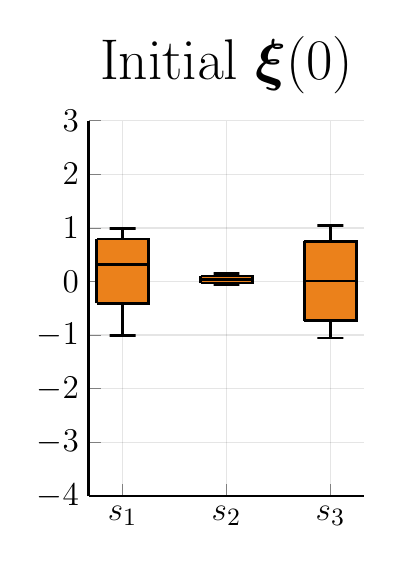
\begin{tikzpicture}[]
\begin{axis}[height = {63.5mm}, ylabel = {}, title = {Initial $\bm \xi(0)$}, xmin = {0.175}, xmax = {2.825}, ymax = {3}, xlabel = {}, unbounded coords=jump,scaled x ticks = false,xlabel style = {font = {\fontsize{18 pt}{23.400000000000002 pt}\selectfont}, color = {rgb,1:red,0.00000000;green,0.00000000;blue,0.00000000}, draw opacity = 1.0, rotate = 0.0},xmajorgrids = true,xtick = {0.5,1.5,2.5},xticklabels = {$s_1$,$s_2$,$s_3$},xtick align = inside,xticklabel style = {font = {\fontsize{13 pt}{16.900000000000002 pt}\selectfont}, color = {rgb,1:red,0.00000000;green,0.00000000;blue,0.00000000}, draw opacity = 1.0, rotate = 0.0},x grid style = {color = {rgb,1:red,0.00000000;green,0.00000000;blue,0.00000000},
draw opacity = 0.1,
line width = 0.5,
solid},axis x line* = left,x axis line style = {color = {rgb,1:red,0.00000000;green,0.00000000;blue,0.00000000},
draw opacity = 1.0,
line width = 1,
solid},scaled y ticks = false,ylabel style = {font = {\fontsize{18 pt}{23.400000000000002 pt}\selectfont}, color = {rgb,1:red,0.00000000;green,0.00000000;blue,0.00000000}, draw opacity = 1.0, rotate = 0.0},ymajorgrids = true,ytick = {-4.0,-3.0,-2.0,-1.0,0.0,1.0,2.0,3.0},yticklabels = {$-4$,$-3$,$-2$,$-1$,$0$,$1$,$2$,$3$},ytick align = inside,yticklabel style = {font = {\fontsize{13 pt}{16.900000000000002 pt}\selectfont}, color = {rgb,1:red,0.00000000;green,0.00000000;blue,0.00000000}, draw opacity = 1.0, rotate = 0.0},y grid style = {color = {rgb,1:red,0.00000000;green,0.00000000;blue,0.00000000},
draw opacity = 0.1,
line width = 0.5,
solid},axis y line* = left,y axis line style = {color = {rgb,1:red,0.00000000;green,0.00000000;blue,0.00000000},
draw opacity = 1.0,
line width = 1,
solid},    xshift = 0.0mm,
    yshift = 0.0mm,
    axis background/.style={fill={rgb,1:red,1.00000000;green,1.00000000;blue,1.00000000}}
,title style = {font = {\fontsize{22 pt}{28.6 pt}\selectfont}, color = {rgb,1:red,0.00000000;green,0.00000000;blue,0.00000000}, draw opacity = 1.0, rotate = 0.0},legend style = {color = {rgb,1:red,0.00000000;green,0.00000000;blue,0.00000000},
draw opacity = 1.0,
line width = 1,
solid,fill = {rgb,1:red,1.00000000;green,1.00000000;blue,1.00000000},font = {\fontsize{13 pt}{16.900000000000002 pt}\selectfont}},colorbar style={title=}, ymin = {-4}, width = {50.8mm}]\addplot+ [color = {rgb,1:red,0.00000000;green,0.00000000;blue,0.00000000},
draw opacity = 1.0,
line width = 1,
solid,mark = none,
mark size = 2.0,
mark options = {
    color = {rgb,1:red,0.00000000;green,0.00000000;blue,0.00000000}, draw opacity = 1.0,
    fill = {rgb,1:red,0.92156863;green,0.50588235;blue,0.10588235}, fill opacity = 1.0,
    line width = 1,
    rotate = 0,
    solid
},fill = {rgb,1:red,0.92156863;green,0.50588235;blue,0.10588235}, fill opacity=1.0,forget plot]coordinates {
(0.5, -1.0093852281570435)
(0.375, -1.0093852281570435)
(0.625, -1.0093852281570435)
(0.5, -1.0093852281570435)
(0.5, -0.4064389243721962)
};
\addplot+ [color = {rgb,1:red,0.00000000;green,0.00000000;blue,0.00000000},
draw opacity = 1.0,
line width = 1,
solid,mark = none,
mark size = 2.0,
mark options = {
    color = {rgb,1:red,0.00000000;green,0.00000000;blue,0.00000000}, draw opacity = 1.0,
    fill = {rgb,1:red,0.92156863;green,0.50588235;blue,0.10588235}, fill opacity = 1.0,
    line width = 1,
    rotate = 0,
    solid
},fill = {rgb,1:red,0.92156863;green,0.50588235;blue,0.10588235}, fill opacity=1.0,forget plot]coordinates {
(0.25, -0.4064389243721962)
(0.25, 0.3174552619457245)
(0.75, 0.3174552619457245)
(0.75, -0.4064389243721962)
(0.25, -0.4064389243721962)
};
\addplot+ [color = {rgb,1:red,0.00000000;green,0.00000000;blue,0.00000000},
draw opacity = 1.0,
line width = 1,
solid,mark = none,
mark size = 2.0,
mark options = {
    color = {rgb,1:red,0.00000000;green,0.00000000;blue,0.00000000}, draw opacity = 1.0,
    fill = {rgb,1:red,0.92156863;green,0.50588235;blue,0.10588235}, fill opacity = 1.0,
    line width = 1,
    rotate = 0,
    solid
},fill = {rgb,1:red,0.92156863;green,0.50588235;blue,0.10588235}, fill opacity=1.0,forget plot]coordinates {
(0.25, 0.7902185618877411)
(0.25, 0.3174552619457245)
(0.75, 0.3174552619457245)
(0.75, 0.7902185618877411)
(0.25, 0.7902185618877411)
};
\addplot+ [color = {rgb,1:red,0.00000000;green,0.00000000;blue,0.00000000},
draw opacity = 1.0,
line width = 1,
solid,mark = none,
mark size = 2.0,
mark options = {
    color = {rgb,1:red,0.00000000;green,0.00000000;blue,0.00000000}, draw opacity = 1.0,
    fill = {rgb,1:red,0.92156863;green,0.50588235;blue,0.10588235}, fill opacity = 1.0,
    line width = 1,
    rotate = 0,
    solid
},fill = {rgb,1:red,0.92156863;green,0.50588235;blue,0.10588235}, fill opacity=1.0,forget plot]coordinates {
(0.5, 0.9865884780883789)
(0.375, 0.9865884780883789)
(0.625, 0.9865884780883789)
(0.5, 0.9865884780883789)
(0.5, 0.7902185618877411)
};
\addplot+ [color = {rgb,1:red,0.00000000;green,0.00000000;blue,0.00000000},
draw opacity = 1.0,
line width = 1,
solid,mark = none,
mark size = 2.0,
mark options = {
    color = {rgb,1:red,0.00000000;green,0.00000000;blue,0.00000000}, draw opacity = 1.0,
    fill = {rgb,1:red,0.92156863;green,0.50588235;blue,0.10588235}, fill opacity = 1.0,
    line width = 1,
    rotate = 0,
    solid
},fill = {rgb,1:red,0.92156863;green,0.50588235;blue,0.10588235}, fill opacity=1.0,forget plot]coordinates {
(1.5, -0.06516765803098679)
(1.375, -0.06516765803098679)
(1.625, -0.06516765803098679)
(1.5, -0.06516765803098679)
(1.5, -0.028776861261576414)
};
\addplot+ [color = {rgb,1:red,0.00000000;green,0.00000000;blue,0.00000000},
draw opacity = 1.0,
line width = 1,
solid,mark = none,
mark size = 2.0,
mark options = {
    color = {rgb,1:red,0.00000000;green,0.00000000;blue,0.00000000}, draw opacity = 1.0,
    fill = {rgb,1:red,0.92156863;green,0.50588235;blue,0.10588235}, fill opacity = 1.0,
    line width = 1,
    rotate = 0,
    solid
},fill = {rgb,1:red,0.92156863;green,0.50588235;blue,0.10588235}, fill opacity=1.0,forget plot]coordinates {
(1.25, -0.028776861261576414)
(1.25, 0.03745450638234615)
(1.75, 0.03745450638234615)
(1.75, -0.028776861261576414)
(1.25, -0.028776861261576414)
};
\addplot+ [color = {rgb,1:red,0.00000000;green,0.00000000;blue,0.00000000},
draw opacity = 1.0,
line width = 1,
solid,mark = none,
mark size = 2.0,
mark options = {
    color = {rgb,1:red,0.00000000;green,0.00000000;blue,0.00000000}, draw opacity = 1.0,
    fill = {rgb,1:red,0.92156863;green,0.50588235;blue,0.10588235}, fill opacity = 1.0,
    line width = 1,
    rotate = 0,
    solid
},fill = {rgb,1:red,0.92156863;green,0.50588235;blue,0.10588235}, fill opacity=1.0,forget plot]coordinates {
(1.25, 0.10362245701253414)
(1.25, 0.03745450638234615)
(1.75, 0.03745450638234615)
(1.75, 0.10362245701253414)
(1.25, 0.10362245701253414)
};
\addplot+ [color = {rgb,1:red,0.00000000;green,0.00000000;blue,0.00000000},
draw opacity = 1.0,
line width = 1,
solid,mark = none,
mark size = 2.0,
mark options = {
    color = {rgb,1:red,0.00000000;green,0.00000000;blue,0.00000000}, draw opacity = 1.0,
    fill = {rgb,1:red,0.92156863;green,0.50588235;blue,0.10588235}, fill opacity = 1.0,
    line width = 1,
    rotate = 0,
    solid
},fill = {rgb,1:red,0.92156863;green,0.50588235;blue,0.10588235}, fill opacity=1.0,forget plot]coordinates {
(1.5, 0.1513187438249588)
(1.375, 0.1513187438249588)
(1.625, 0.1513187438249588)
(1.5, 0.1513187438249588)
(1.5, 0.10362245701253414)
};
\addplot+ [color = {rgb,1:red,0.00000000;green,0.00000000;blue,0.00000000},
draw opacity = 1.0,
line width = 1,
solid,mark = none,
mark size = 2.0,
mark options = {
    color = {rgb,1:red,0.00000000;green,0.00000000;blue,0.00000000}, draw opacity = 1.0,
    fill = {rgb,1:red,0.92156863;green,0.50588235;blue,0.10588235}, fill opacity = 1.0,
    line width = 1,
    rotate = 0,
    solid
},fill = {rgb,1:red,0.92156863;green,0.50588235;blue,0.10588235}, fill opacity=1.0,forget plot]coordinates {
(2.5, -1.055550456047058)
(2.375, -1.055550456047058)
(2.625, -1.055550456047058)
(2.5, -1.055550456047058)
(2.5, -0.7337391972541809)
};
\addplot+ [color = {rgb,1:red,0.00000000;green,0.00000000;blue,0.00000000},
draw opacity = 1.0,
line width = 1,
solid,mark = none,
mark size = 2.0,
mark options = {
    color = {rgb,1:red,0.00000000;green,0.00000000;blue,0.00000000}, draw opacity = 1.0,
    fill = {rgb,1:red,0.92156863;green,0.50588235;blue,0.10588235}, fill opacity = 1.0,
    line width = 1,
    rotate = 0,
    solid
},fill = {rgb,1:red,0.92156863;green,0.50588235;blue,0.10588235}, fill opacity=1.0,forget plot]coordinates {
(2.25, -0.7337391972541809)
(2.25, 0.007332766428589821)
(2.75, 0.007332766428589821)
(2.75, -0.7337391972541809)
(2.25, -0.7337391972541809)
};
\addplot+ [color = {rgb,1:red,0.00000000;green,0.00000000;blue,0.00000000},
draw opacity = 1.0,
line width = 1,
solid,mark = none,
mark size = 2.0,
mark options = {
    color = {rgb,1:red,0.00000000;green,0.00000000;blue,0.00000000}, draw opacity = 1.0,
    fill = {rgb,1:red,0.92156863;green,0.50588235;blue,0.10588235}, fill opacity = 1.0,
    line width = 1,
    rotate = 0,
    solid
},fill = {rgb,1:red,0.92156863;green,0.50588235;blue,0.10588235}, fill opacity=1.0,forget plot]coordinates {
(2.25, 0.7472901940345764)
(2.25, 0.007332766428589821)
(2.75, 0.007332766428589821)
(2.75, 0.7472901940345764)
(2.25, 0.7472901940345764)
};
\addplot+ [color = {rgb,1:red,0.00000000;green,0.00000000;blue,0.00000000},
draw opacity = 1.0,
line width = 1,
solid,mark = none,
mark size = 2.0,
mark options = {
    color = {rgb,1:red,0.00000000;green,0.00000000;blue,0.00000000}, draw opacity = 1.0,
    fill = {rgb,1:red,0.92156863;green,0.50588235;blue,0.10588235}, fill opacity = 1.0,
    line width = 1,
    rotate = 0,
    solid
},fill = {rgb,1:red,0.92156863;green,0.50588235;blue,0.10588235}, fill opacity=1.0,forget plot]coordinates {
(2.5, 1.0507506132125854)
(2.375, 1.0507506132125854)
(2.625, 1.0507506132125854)
(2.5, 1.0507506132125854)
(2.5, 0.7472901940345764)
};
\end{axis}

\end{tikzpicture}
}
  \resizebox{!}{.28\linewidth}{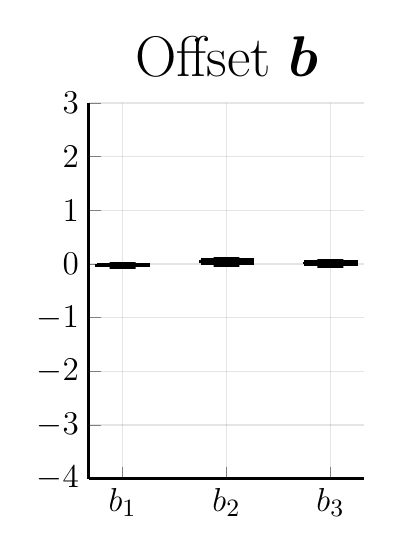
\begin{tikzpicture}[]
\begin{axis}[height = {63.5mm}, ylabel = {}, title = {Offset $\bm b$}, xmin = {0.175}, xmax = {2.825}, ymax = {3}, xlabel = {}, unbounded coords=jump,scaled x ticks = false,xlabel style = {font = {\fontsize{18 pt}{23.400000000000002 pt}\selectfont}, color = {rgb,1:red,0.00000000;green,0.00000000;blue,0.00000000}, draw opacity = 1.0, rotate = 0.0},xmajorgrids = true,xtick = {0.5,1.5,2.5},xticklabels = {$b_1$,$b_2$,$b_3$},xtick align = inside,xticklabel style = {font = {\fontsize{13 pt}{16.900000000000002 pt}\selectfont}, color = {rgb,1:red,0.00000000;green,0.00000000;blue,0.00000000}, draw opacity = 1.0, rotate = 0.0},x grid style = {color = {rgb,1:red,0.00000000;green,0.00000000;blue,0.00000000},
draw opacity = 0.1,
line width = 0.5,
solid},axis x line* = left,x axis line style = {color = {rgb,1:red,0.00000000;green,0.00000000;blue,0.00000000},
draw opacity = 1.0,
line width = 1,
solid},scaled y ticks = false,ylabel style = {font = {\fontsize{18 pt}{23.400000000000002 pt}\selectfont}, color = {rgb,1:red,0.00000000;green,0.00000000;blue,0.00000000}, draw opacity = 1.0, rotate = 0.0},ymajorgrids = true,ytick = {-4.0,-3.0,-2.0,-1.0,0.0,1.0,2.0,3.0},yticklabels = {$-4$,$-3$,$-2$,$-1$,$0$,$1$,$2$,$3$},ytick align = inside,yticklabel style = {font = {\fontsize{13 pt}{16.900000000000002 pt}\selectfont}, color = {rgb,1:red,0.00000000;green,0.00000000;blue,0.00000000}, draw opacity = 1.0, rotate = 0.0},y grid style = {color = {rgb,1:red,0.00000000;green,0.00000000;blue,0.00000000},
draw opacity = 0.1,
line width = 0.5,
solid},axis y line* = left,y axis line style = {color = {rgb,1:red,0.00000000;green,0.00000000;blue,0.00000000},
draw opacity = 1.0,
line width = 1,
solid},    xshift = 0.0mm,
    yshift = 0.0mm,
    axis background/.style={fill={rgb,1:red,1.00000000;green,1.00000000;blue,1.00000000}}
,title style = {font = {\fontsize{22 pt}{28.6 pt}\selectfont}, color = {rgb,1:red,0.00000000;green,0.00000000;blue,0.00000000}, draw opacity = 1.0, rotate = 0.0},legend style = {color = {rgb,1:red,0.00000000;green,0.00000000;blue,0.00000000},
draw opacity = 1.0,
line width = 1,
solid,fill = {rgb,1:red,1.00000000;green,1.00000000;blue,1.00000000},font = {\fontsize{13 pt}{16.900000000000002 pt}\selectfont}},colorbar style={title=}, ymin = {-4}, width = {50.8mm}]\addplot+ [color = {rgb,1:red,0.00000000;green,0.00000000;blue,0.00000000},
draw opacity = 1.0,
line width = 1,
solid,mark = none,
mark size = 2.0,
mark options = {
    color = {rgb,1:red,0.00000000;green,0.00000000;blue,0.00000000}, draw opacity = 1.0,
    fill = {rgb,1:red,0.92156863;green,0.50588235;blue,0.10588235}, fill opacity = 1.0,
    line width = 1,
    rotate = 0,
    solid
},fill = {rgb,1:red,0.92156863;green,0.50588235;blue,0.10588235}, fill opacity=1.0,forget plot]coordinates {
(0.5, -0.07128085196018219)
(0.375, -0.07128085196018219)
(0.625, -0.07128085196018219)
(0.5, -0.07128085196018219)
(0.5, -0.03508143872022629)
};
\addplot+ [color = {rgb,1:red,0.00000000;green,0.00000000;blue,0.00000000},
draw opacity = 1.0,
line width = 1,
solid,mark = none,
mark size = 2.0,
mark options = {
    color = {rgb,1:red,0.00000000;green,0.00000000;blue,0.00000000}, draw opacity = 1.0,
    fill = {rgb,1:red,0.92156863;green,0.50588235;blue,0.10588235}, fill opacity = 1.0,
    line width = 1,
    rotate = 0,
    solid
},fill = {rgb,1:red,0.92156863;green,0.50588235;blue,0.10588235}, fill opacity=1.0,forget plot]coordinates {
(0.25, -0.03508143872022629)
(0.25, -0.023331661708652973)
(0.75, -0.023331661708652973)
(0.75, -0.03508143872022629)
(0.25, -0.03508143872022629)
};
\addplot+ [color = {rgb,1:red,0.00000000;green,0.00000000;blue,0.00000000},
draw opacity = 1.0,
line width = 1,
solid,mark = none,
mark size = 2.0,
mark options = {
    color = {rgb,1:red,0.00000000;green,0.00000000;blue,0.00000000}, draw opacity = 1.0,
    fill = {rgb,1:red,0.92156863;green,0.50588235;blue,0.10588235}, fill opacity = 1.0,
    line width = 1,
    rotate = 0,
    solid
},fill = {rgb,1:red,0.92156863;green,0.50588235;blue,0.10588235}, fill opacity=1.0,forget plot]coordinates {
(0.25, -0.01039293222129345)
(0.25, -0.023331661708652973)
(0.75, -0.023331661708652973)
(0.75, -0.01039293222129345)
(0.25, -0.01039293222129345)
};
\addplot+ [color = {rgb,1:red,0.00000000;green,0.00000000;blue,0.00000000},
draw opacity = 1.0,
line width = 1,
solid,mark = none,
mark size = 2.0,
mark options = {
    color = {rgb,1:red,0.00000000;green,0.00000000;blue,0.00000000}, draw opacity = 1.0,
    fill = {rgb,1:red,0.92156863;green,0.50588235;blue,0.10588235}, fill opacity = 1.0,
    line width = 1,
    rotate = 0,
    solid
},fill = {rgb,1:red,0.92156863;green,0.50588235;blue,0.10588235}, fill opacity=1.0,forget plot]coordinates {
(0.5, 0.019218027591705322)
(0.375, 0.019218027591705322)
(0.625, 0.019218027591705322)
(0.5, 0.019218027591705322)
(0.5, -0.01039293222129345)
};
\addplot+ [color = {rgb,1:red,0.00000000;green,0.00000000;blue,0.00000000},
draw opacity = 1.0,
line width = 1,
solid,mark = none,
mark size = 2.0,
mark options = {
    color = {rgb,1:red,0.00000000;green,0.00000000;blue,0.00000000}, draw opacity = 1.0,
    fill = {rgb,1:red,0.92156863;green,0.50588235;blue,0.10588235}, fill opacity = 1.0,
    line width = 1,
    rotate = 0,
    solid
},fill = {rgb,1:red,0.92156863;green,0.50588235;blue,0.10588235}, fill opacity=1.0,forget plot]coordinates {
(1.5, -0.020190563052892685)
(1.375, -0.020190563052892685)
(1.625, -0.020190563052892685)
(1.5, -0.020190563052892685)
(1.5, 0.011186720803380013)
};
\addplot+ [color = {rgb,1:red,0.00000000;green,0.00000000;blue,0.00000000},
draw opacity = 1.0,
line width = 1,
solid,mark = none,
mark size = 2.0,
mark options = {
    color = {rgb,1:red,0.00000000;green,0.00000000;blue,0.00000000}, draw opacity = 1.0,
    fill = {rgb,1:red,0.92156863;green,0.50588235;blue,0.10588235}, fill opacity = 1.0,
    line width = 1,
    rotate = 0,
    solid
},fill = {rgb,1:red,0.92156863;green,0.50588235;blue,0.10588235}, fill opacity=1.0,forget plot]coordinates {
(1.25, 0.011186720803380013)
(1.25, 0.04952448979020119)
(1.75, 0.04952448979020119)
(1.75, 0.011186720803380013)
(1.25, 0.011186720803380013)
};
\addplot+ [color = {rgb,1:red,0.00000000;green,0.00000000;blue,0.00000000},
draw opacity = 1.0,
line width = 1,
solid,mark = none,
mark size = 2.0,
mark options = {
    color = {rgb,1:red,0.00000000;green,0.00000000;blue,0.00000000}, draw opacity = 1.0,
    fill = {rgb,1:red,0.92156863;green,0.50588235;blue,0.10588235}, fill opacity = 1.0,
    line width = 1,
    rotate = 0,
    solid
},fill = {rgb,1:red,0.92156863;green,0.50588235;blue,0.10588235}, fill opacity=1.0,forget plot]coordinates {
(1.25, 0.08388775587081909)
(1.25, 0.04952448979020119)
(1.75, 0.04952448979020119)
(1.75, 0.08388775587081909)
(1.25, 0.08388775587081909)
};
\addplot+ [color = {rgb,1:red,0.00000000;green,0.00000000;blue,0.00000000},
draw opacity = 1.0,
line width = 1,
solid,mark = none,
mark size = 2.0,
mark options = {
    color = {rgb,1:red,0.00000000;green,0.00000000;blue,0.00000000}, draw opacity = 1.0,
    fill = {rgb,1:red,0.92156863;green,0.50588235;blue,0.10588235}, fill opacity = 1.0,
    line width = 1,
    rotate = 0,
    solid
},fill = {rgb,1:red,0.92156863;green,0.50588235;blue,0.10588235}, fill opacity=1.0,forget plot]coordinates {
(1.5, 0.10372693836688995)
(1.375, 0.10372693836688995)
(1.625, 0.10372693836688995)
(1.5, 0.10372693836688995)
(1.5, 0.08388775587081909)
};
\addplot+ [color = {rgb,1:red,0.00000000;green,0.00000000;blue,0.00000000},
draw opacity = 1.0,
line width = 1,
solid,mark = none,
mark size = 2.0,
mark options = {
    color = {rgb,1:red,0.00000000;green,0.00000000;blue,0.00000000}, draw opacity = 1.0,
    fill = {rgb,1:red,0.92156863;green,0.50588235;blue,0.10588235}, fill opacity = 1.0,
    line width = 1,
    rotate = 0,
    solid
},fill = {rgb,1:red,0.92156863;green,0.50588235;blue,0.10588235}, fill opacity=1.0,forget plot]coordinates {
(2.5, -0.04140687361359596)
(2.375, -0.04140687361359596)
(2.625, -0.04140687361359596)
(2.5, -0.04140687361359596)
(2.5, -0.006251898128539324)
};
\addplot+ [color = {rgb,1:red,0.00000000;green,0.00000000;blue,0.00000000},
draw opacity = 1.0,
line width = 1,
solid,mark = none,
mark size = 2.0,
mark options = {
    color = {rgb,1:red,0.00000000;green,0.00000000;blue,0.00000000}, draw opacity = 1.0,
    fill = {rgb,1:red,0.92156863;green,0.50588235;blue,0.10588235}, fill opacity = 1.0,
    line width = 1,
    rotate = 0,
    solid
},fill = {rgb,1:red,0.92156863;green,0.50588235;blue,0.10588235}, fill opacity=1.0,forget plot]coordinates {
(2.25, -0.006251898128539324)
(2.25, 0.02104303054511547)
(2.75, 0.02104303054511547)
(2.75, -0.006251898128539324)
(2.25, -0.006251898128539324)
};
\addplot+ [color = {rgb,1:red,0.00000000;green,0.00000000;blue,0.00000000},
draw opacity = 1.0,
line width = 1,
solid,mark = none,
mark size = 2.0,
mark options = {
    color = {rgb,1:red,0.00000000;green,0.00000000;blue,0.00000000}, draw opacity = 1.0,
    fill = {rgb,1:red,0.92156863;green,0.50588235;blue,0.10588235}, fill opacity = 1.0,
    line width = 1,
    rotate = 0,
    solid
},fill = {rgb,1:red,0.92156863;green,0.50588235;blue,0.10588235}, fill opacity=1.0,forget plot]coordinates {
(2.25, 0.041737623512744904)
(2.25, 0.02104303054511547)
(2.75, 0.02104303054511547)
(2.75, 0.041737623512744904)
(2.25, 0.041737623512744904)
};
\addplot+ [color = {rgb,1:red,0.00000000;green,0.00000000;blue,0.00000000},
draw opacity = 1.0,
line width = 1,
solid,mark = none,
mark size = 2.0,
mark options = {
    color = {rgb,1:red,0.00000000;green,0.00000000;blue,0.00000000}, draw opacity = 1.0,
    fill = {rgb,1:red,0.92156863;green,0.50588235;blue,0.10588235}, fill opacity = 1.0,
    line width = 1,
    rotate = 0,
    solid
},fill = {rgb,1:red,0.92156863;green,0.50588235;blue,0.10588235}, fill opacity=1.0,forget plot]coordinates {
(2.5, 0.07456278800964355)
(2.375, 0.07456278800964355)
(2.625, 0.07456278800964355)
(2.5, 0.07456278800964355)
(2.5, 0.041737623512744904)
};
\end{axis}

\end{tikzpicture}
}
  \color{black} % fix white text color
  \begin{align*}
    \begin{bmatrix}
      \dot{\xi} \\ \ddot{\xi} \\ \dddot{\xi}
    \end{bmatrix}
    &=
    \begin{bmatrix}
      0 & 0 & 1\\
      0 & 0 & 0\\
      -\omega^2 & 0 & 0
    \end{bmatrix}
    \begin{bmatrix}
      \xi \\ 0 \\ \dot{\xi}
    \end{bmatrix}
    +
    \begin{bmatrix}
      0 \\ 0 \\ 0
    \end{bmatrix}
  \end{align*}

  \begin{block}{Successful model identification}
    \textbf{But}: 1-3 irrelevent parameters remain in $\bm W$
  \end{block}
\end{frame}

\begin{frame}{Rodent - VAE + ODE solver + ARD}
  \centering
  \def\layersep{2.6cm}
  \begin{tikzpicture}[shorten >=1pt,->,draw=black!50, node distance=\layersep]
    \tikzstyle{every pin edge}=[<-,shorten <=1pt]
    \tikzstyle{neuron}=[circle,fill=black!25,minimum size=17pt,inner sep=0pt]
    \tikzstyle{input neuron}=[neuron, fill=gray];
    \tikzstyle{output neuron}=[neuron, fill=gray];
    \tikzstyle{hidden neuron}=[neuron, fill=mLightBrown];
    \tikzstyle{annot} = [text width=4em, text centered]
  
    % Draw the hidden layer nodes
    \node[hidden neuron] (H-1) at (\layersep,-2cm) {$\bm W$};
    \node[hidden neuron] (H-2) at (\layersep,-3cm) {$\bm \xi$};
    \node[hidden neuron] (H-3) at (\layersep,-4cm) {$\bm b$};
  
    % Draw the output layer node
    \foreach \name / \y in {1,...,5}
        \node[output neuron] (O-\name) at (\layersep*2,-\y cm) {};
  
    % draw and connect decoder
    \node[draw, ultra thick, rotate=90, rounded corners=8, minimum height=1.1cm, minimum width=3.5cm]
        (odesolve) at  (\layersep+\layersep/2, -3) {ODE solver $\psi$};
    \foreach \name / \y in {1,...,3}
        \path (H-\name) edge (odesolve);
    \foreach \dest in {1,...,5}
        \path (odesolve) edge (O-\dest);
  
    % Annotate the last layer
    \node[above of=O-3] (pxz) {$\bm x = \psi(\bm z) + \sigma_x$};
  
    % output lines
    \draw[-,dotted, very thick, decoration={snake, segment length=0.32cm, amplitude=0.6cm}, decorate]
      (\layersep*2+0.5cm, -1.5) -- (\layersep*2+2cm, -1.5);
    \draw[-,dotted, very thick, decoration={snake, segment length=1.3cm, amplitude=0.6cm}, decorate]
      (\layersep*2+0.5cm, -3) -- (\layersep*2+2cm, -3);
    \draw[-,dotted, very thick, decoration={snake, segment length=0.7cm, amplitude=0.6cm}, decorate]
      (\layersep*2+0.5cm, -4.5) -- (\layersep*2+2cm, -4.5);

    % Draw the input layer nodes
    \foreach \name / \y in {1,...,5}
    % This is the same as writing \foreach \name / \y in {1/1,2/2,3/3,4/4}
      \node[input neuron] (I-\name) at (0,-\y) {};

    % Connect every node in the input layer with every node in the
    % hidden layer.
    \foreach \source in {1,...,5}
        \foreach \dest in {1,...,3}
            \path (I-\source) edge (H-\dest);

    \draw[-, very thick, decoration={snake, segment length=0.32cm, amplitude=0.6cm}, decorate]
      (-2cm, -1.5) -- (-0.5cm, -1.5);
    \draw[-, very thick, decoration={snake, segment length=1.3cm, amplitude=0.6cm}, decorate]
      (-2cm, -3) -- (-0.5cm, -3);
    \draw[-, very thick, decoration={snake, segment length=0.7cm, amplitude=0.6cm}, decorate]
      (-2cm, -4.5) -- (-0.5cm, -4.5);

    \node[above of=I-3] (pzx) {$\bm z = \phi_\theta(\bm x) + \bm \sigma_z$};
    \node[annot, below of=H-1] (pzx) {$\mathcal{N}(0, \lambda_z)$};
  \end{tikzpicture}
\end{frame}


\note{
  \begin{itemize}
    \item hierarchical model
    \item enforces sparsity
  \end{itemize}
  
  I am not sure how deep to go here. is it confusing to just show the equations
  and say that ARD is our main workhorse?

ODE adds explainability. we can now identify a \alert{physics motivated}
manifold of harmonic signals}


\begin{frame}{Results}
  \resizebox{!}{.28\linewidth}{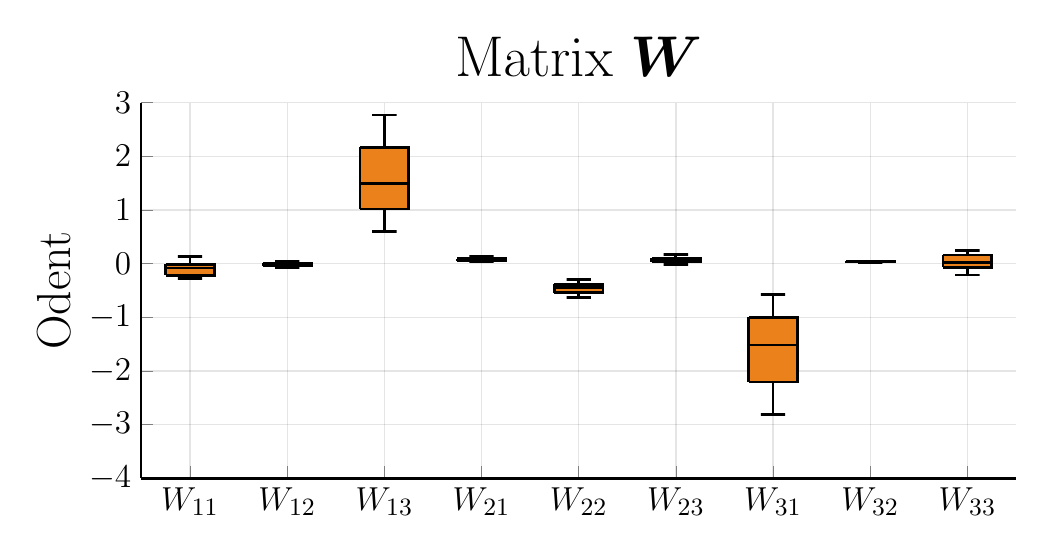
\begin{tikzpicture}[]
\begin{axis}[height = {63.5mm}, ylabel = {Odent}, title = {Matrix $\bm W$}, xmin = {-0.0050000000000000044}, xmax = {9.005}, ymax = {3}, xlabel = {}, unbounded coords=jump,scaled x ticks = false,xlabel style = {font = {\fontsize{18 pt}{23.400000000000002 pt}\selectfont}, color = {rgb,1:red,0.00000000;green,0.00000000;blue,0.00000000}, draw opacity = 1.0, rotate = 0.0},xmajorgrids = true,xtick = {0.5,1.5,2.5,3.5,4.5,5.5,6.5,7.5,8.5},xticklabels = {$W_{11}$,$W_{12}$,$W_{13}$,$W_{21}$,$W_{22}$,$W_{23}$,$W_{31}$,$W_{32}$,$W_{33}$},xtick align = inside,xticklabel style = {font = {\fontsize{13 pt}{16.900000000000002 pt}\selectfont}, color = {rgb,1:red,0.00000000;green,0.00000000;blue,0.00000000}, draw opacity = 1.0, rotate = 0.0},x grid style = {color = {rgb,1:red,0.00000000;green,0.00000000;blue,0.00000000},
draw opacity = 0.1,
line width = 0.5,
solid},axis x line* = left,x axis line style = {color = {rgb,1:red,0.00000000;green,0.00000000;blue,0.00000000},
draw opacity = 1.0,
line width = 1,
solid},scaled y ticks = false,ylabel style = {font = {\fontsize{18 pt}{23.400000000000002 pt}\selectfont}, color = {rgb,1:red,0.00000000;green,0.00000000;blue,0.00000000}, draw opacity = 1.0, rotate = 0.0},ymajorgrids = true,ytick = {-4.0,-3.0,-2.0,-1.0,0.0,1.0,2.0,3.0},yticklabels = {$-4$,$-3$,$-2$,$-1$,$0$,$1$,$2$,$3$},ytick align = inside,yticklabel style = {font = {\fontsize{13 pt}{16.900000000000002 pt}\selectfont}, color = {rgb,1:red,0.00000000;green,0.00000000;blue,0.00000000}, draw opacity = 1.0, rotate = 0.0},y grid style = {color = {rgb,1:red,0.00000000;green,0.00000000;blue,0.00000000},
draw opacity = 0.1,
line width = 0.5,
solid},axis y line* = left,y axis line style = {color = {rgb,1:red,0.00000000;green,0.00000000;blue,0.00000000},
draw opacity = 1.0,
line width = 1,
solid},    xshift = 0.0mm,
    yshift = 0.0mm,
    axis background/.style={fill={rgb,1:red,1.00000000;green,1.00000000;blue,1.00000000}}
,title style = {font = {\fontsize{22 pt}{28.6 pt}\selectfont}, color = {rgb,1:red,0.00000000;green,0.00000000;blue,0.00000000}, draw opacity = 1.0, rotate = 0.0},legend style = {color = {rgb,1:red,0.00000000;green,0.00000000;blue,0.00000000},
draw opacity = 1.0,
line width = 1,
solid,fill = {rgb,1:red,1.00000000;green,1.00000000;blue,1.00000000},font = {\fontsize{13 pt}{16.900000000000002 pt}\selectfont}},colorbar style={title=}, ymin = {-4}, width = {127.0mm}]\addplot+ [color = {rgb,1:red,0.00000000;green,0.00000000;blue,0.00000000},
draw opacity = 1.0,
line width = 1,
solid,mark = none,
mark size = 2.0,
mark options = {
    color = {rgb,1:red,0.00000000;green,0.00000000;blue,0.00000000}, draw opacity = 1.0,
    fill = {rgb,1:red,0.92156863;green,0.50588235;blue,0.10588235}, fill opacity = 1.0,
    line width = 1,
    rotate = 0,
    solid
},fill = {rgb,1:red,0.92156863;green,0.50588235;blue,0.10588235}, fill opacity=1.0,forget plot]coordinates {
(0.5, -0.28068220615386963)
(0.375, -0.28068220615386963)
(0.625, -0.28068220615386963)
(0.5, -0.28068220615386963)
(0.5, -0.21647277101874352)
};
\addplot+ [color = {rgb,1:red,0.00000000;green,0.00000000;blue,0.00000000},
draw opacity = 1.0,
line width = 1,
solid,mark = none,
mark size = 2.0,
mark options = {
    color = {rgb,1:red,0.00000000;green,0.00000000;blue,0.00000000}, draw opacity = 1.0,
    fill = {rgb,1:red,0.92156863;green,0.50588235;blue,0.10588235}, fill opacity = 1.0,
    line width = 1,
    rotate = 0,
    solid
},fill = {rgb,1:red,0.92156863;green,0.50588235;blue,0.10588235}, fill opacity=1.0,forget plot]coordinates {
(0.25, -0.21647277101874352)
(0.25, -0.08380848169326782)
(0.75, -0.08380848169326782)
(0.75, -0.21647277101874352)
(0.25, -0.21647277101874352)
};
\addplot+ [color = {rgb,1:red,0.00000000;green,0.00000000;blue,0.00000000},
draw opacity = 1.0,
line width = 1,
solid,mark = none,
mark size = 2.0,
mark options = {
    color = {rgb,1:red,0.00000000;green,0.00000000;blue,0.00000000}, draw opacity = 1.0,
    fill = {rgb,1:red,0.92156863;green,0.50588235;blue,0.10588235}, fill opacity = 1.0,
    line width = 1,
    rotate = 0,
    solid
},fill = {rgb,1:red,0.92156863;green,0.50588235;blue,0.10588235}, fill opacity=1.0,forget plot]coordinates {
(0.25, -0.011269278824329376)
(0.25, -0.08380848169326782)
(0.75, -0.08380848169326782)
(0.75, -0.011269278824329376)
(0.25, -0.011269278824329376)
};
\addplot+ [color = {rgb,1:red,0.00000000;green,0.00000000;blue,0.00000000},
draw opacity = 1.0,
line width = 1,
solid,mark = none,
mark size = 2.0,
mark options = {
    color = {rgb,1:red,0.00000000;green,0.00000000;blue,0.00000000}, draw opacity = 1.0,
    fill = {rgb,1:red,0.92156863;green,0.50588235;blue,0.10588235}, fill opacity = 1.0,
    line width = 1,
    rotate = 0,
    solid
},fill = {rgb,1:red,0.92156863;green,0.50588235;blue,0.10588235}, fill opacity=1.0,forget plot]coordinates {
(0.5, 0.1312718391418457)
(0.375, 0.1312718391418457)
(0.625, 0.1312718391418457)
(0.5, 0.1312718391418457)
(0.5, -0.011269278824329376)
};
\addplot+ [color = {rgb,1:red,0.00000000;green,0.00000000;blue,0.00000000},
draw opacity = 1.0,
line width = 1,
solid,mark = none,
mark size = 2.0,
mark options = {
    color = {rgb,1:red,0.00000000;green,0.00000000;blue,0.00000000}, draw opacity = 1.0,
    fill = {rgb,1:red,0.92156863;green,0.50588235;blue,0.10588235}, fill opacity = 1.0,
    line width = 1,
    rotate = 0,
    solid
},fill = {rgb,1:red,0.92156863;green,0.50588235;blue,0.10588235}, fill opacity=1.0,forget plot]coordinates {
(1.5, -0.08050356060266495)
(1.375, -0.08050356060266495)
(1.625, -0.08050356060266495)
(1.5, -0.08050356060266495)
(1.5, -0.035347397439181805)
};
\addplot+ [color = {rgb,1:red,0.00000000;green,0.00000000;blue,0.00000000},
draw opacity = 1.0,
line width = 1,
solid,mark = none,
mark size = 2.0,
mark options = {
    color = {rgb,1:red,0.00000000;green,0.00000000;blue,0.00000000}, draw opacity = 1.0,
    fill = {rgb,1:red,0.92156863;green,0.50588235;blue,0.10588235}, fill opacity = 1.0,
    line width = 1,
    rotate = 0,
    solid
},fill = {rgb,1:red,0.92156863;green,0.50588235;blue,0.10588235}, fill opacity=1.0,forget plot]coordinates {
(1.25, -0.035347397439181805)
(1.25, -0.015371293295174837)
(1.75, -0.015371293295174837)
(1.75, -0.035347397439181805)
(1.25, -0.035347397439181805)
};
\addplot+ [color = {rgb,1:red,0.00000000;green,0.00000000;blue,0.00000000},
draw opacity = 1.0,
line width = 1,
solid,mark = none,
mark size = 2.0,
mark options = {
    color = {rgb,1:red,0.00000000;green,0.00000000;blue,0.00000000}, draw opacity = 1.0,
    fill = {rgb,1:red,0.92156863;green,0.50588235;blue,0.10588235}, fill opacity = 1.0,
    line width = 1,
    rotate = 0,
    solid
},fill = {rgb,1:red,0.92156863;green,0.50588235;blue,0.10588235}, fill opacity=1.0,forget plot]coordinates {
(1.25, 0.006936707533895969)
(1.25, -0.015371293295174837)
(1.75, -0.015371293295174837)
(1.75, 0.006936707533895969)
(1.25, 0.006936707533895969)
};
\addplot+ [color = {rgb,1:red,0.00000000;green,0.00000000;blue,0.00000000},
draw opacity = 1.0,
line width = 1,
solid,mark = none,
mark size = 2.0,
mark options = {
    color = {rgb,1:red,0.00000000;green,0.00000000;blue,0.00000000}, draw opacity = 1.0,
    fill = {rgb,1:red,0.92156863;green,0.50588235;blue,0.10588235}, fill opacity = 1.0,
    line width = 1,
    rotate = 0,
    solid
},fill = {rgb,1:red,0.92156863;green,0.50588235;blue,0.10588235}, fill opacity=1.0,forget plot]coordinates {
(1.5, 0.043295323848724365)
(1.375, 0.043295323848724365)
(1.625, 0.043295323848724365)
(1.5, 0.043295323848724365)
(1.5, 0.006936707533895969)
};
\addplot+ [color = {rgb,1:red,0.00000000;green,0.00000000;blue,0.00000000},
draw opacity = 1.0,
line width = 1,
solid,mark = none,
mark size = 2.0,
mark options = {
    color = {rgb,1:red,0.00000000;green,0.00000000;blue,0.00000000}, draw opacity = 1.0,
    fill = {rgb,1:red,0.92156863;green,0.50588235;blue,0.10588235}, fill opacity = 1.0,
    line width = 1,
    rotate = 0,
    solid
},fill = {rgb,1:red,0.92156863;green,0.50588235;blue,0.10588235}, fill opacity=1.0,forget plot]coordinates {
(2.5, 0.5995415449142456)
(2.375, 0.5995415449142456)
(2.625, 0.5995415449142456)
(2.5, 0.5995415449142456)
(2.5, 1.0167028605937958)
};
\addplot+ [color = {rgb,1:red,0.00000000;green,0.00000000;blue,0.00000000},
draw opacity = 1.0,
line width = 1,
solid,mark = none,
mark size = 2.0,
mark options = {
    color = {rgb,1:red,0.00000000;green,0.00000000;blue,0.00000000}, draw opacity = 1.0,
    fill = {rgb,1:red,0.92156863;green,0.50588235;blue,0.10588235}, fill opacity = 1.0,
    line width = 1,
    rotate = 0,
    solid
},fill = {rgb,1:red,0.92156863;green,0.50588235;blue,0.10588235}, fill opacity=1.0,forget plot]coordinates {
(2.25, 1.0167028605937958)
(2.25, 1.4863724112510681)
(2.75, 1.4863724112510681)
(2.75, 1.0167028605937958)
(2.25, 1.0167028605937958)
};
\addplot+ [color = {rgb,1:red,0.00000000;green,0.00000000;blue,0.00000000},
draw opacity = 1.0,
line width = 1,
solid,mark = none,
mark size = 2.0,
mark options = {
    color = {rgb,1:red,0.00000000;green,0.00000000;blue,0.00000000}, draw opacity = 1.0,
    fill = {rgb,1:red,0.92156863;green,0.50588235;blue,0.10588235}, fill opacity = 1.0,
    line width = 1,
    rotate = 0,
    solid
},fill = {rgb,1:red,0.92156863;green,0.50588235;blue,0.10588235}, fill opacity=1.0,forget plot]coordinates {
(2.25, 2.1655468344688416)
(2.25, 1.4863724112510681)
(2.75, 1.4863724112510681)
(2.75, 2.1655468344688416)
(2.25, 2.1655468344688416)
};
\addplot+ [color = {rgb,1:red,0.00000000;green,0.00000000;blue,0.00000000},
draw opacity = 1.0,
line width = 1,
solid,mark = none,
mark size = 2.0,
mark options = {
    color = {rgb,1:red,0.00000000;green,0.00000000;blue,0.00000000}, draw opacity = 1.0,
    fill = {rgb,1:red,0.92156863;green,0.50588235;blue,0.10588235}, fill opacity = 1.0,
    line width = 1,
    rotate = 0,
    solid
},fill = {rgb,1:red,0.92156863;green,0.50588235;blue,0.10588235}, fill opacity=1.0,forget plot]coordinates {
(2.5, 2.770195484161377)
(2.375, 2.770195484161377)
(2.625, 2.770195484161377)
(2.5, 2.770195484161377)
(2.5, 2.1655468344688416)
};
\addplot+ [color = {rgb,1:red,0.00000000;green,0.00000000;blue,0.00000000},
draw opacity = 1.0,
line width = 1,
solid,mark = none,
mark size = 2.0,
mark options = {
    color = {rgb,1:red,0.00000000;green,0.00000000;blue,0.00000000}, draw opacity = 1.0,
    fill = {rgb,1:red,0.92156863;green,0.50588235;blue,0.10588235}, fill opacity = 1.0,
    line width = 1,
    rotate = 0,
    solid
},fill = {rgb,1:red,0.92156863;green,0.50588235;blue,0.10588235}, fill opacity=1.0,forget plot]coordinates {
(3.5, 0.029579564929008484)
(3.375, 0.029579564929008484)
(3.625, 0.029579564929008484)
(3.5, 0.029579564929008484)
(3.5, 0.05103161372244358)
};
\addplot+ [color = {rgb,1:red,0.00000000;green,0.00000000;blue,0.00000000},
draw opacity = 1.0,
line width = 1,
solid,mark = none,
mark size = 2.0,
mark options = {
    color = {rgb,1:red,0.00000000;green,0.00000000;blue,0.00000000}, draw opacity = 1.0,
    fill = {rgb,1:red,0.92156863;green,0.50588235;blue,0.10588235}, fill opacity = 1.0,
    line width = 1,
    rotate = 0,
    solid
},fill = {rgb,1:red,0.92156863;green,0.50588235;blue,0.10588235}, fill opacity=1.0,forget plot]coordinates {
(3.25, 0.05103161372244358)
(3.25, 0.06557240709662437)
(3.75, 0.06557240709662437)
(3.75, 0.05103161372244358)
(3.25, 0.05103161372244358)
};
\addplot+ [color = {rgb,1:red,0.00000000;green,0.00000000;blue,0.00000000},
draw opacity = 1.0,
line width = 1,
solid,mark = none,
mark size = 2.0,
mark options = {
    color = {rgb,1:red,0.00000000;green,0.00000000;blue,0.00000000}, draw opacity = 1.0,
    fill = {rgb,1:red,0.92156863;green,0.50588235;blue,0.10588235}, fill opacity = 1.0,
    line width = 1,
    rotate = 0,
    solid
},fill = {rgb,1:red,0.92156863;green,0.50588235;blue,0.10588235}, fill opacity=1.0,forget plot]coordinates {
(3.25, 0.08917277306318283)
(3.25, 0.06557240709662437)
(3.75, 0.06557240709662437)
(3.75, 0.08917277306318283)
(3.25, 0.08917277306318283)
};
\addplot+ [color = {rgb,1:red,0.00000000;green,0.00000000;blue,0.00000000},
draw opacity = 1.0,
line width = 1,
solid,mark = none,
mark size = 2.0,
mark options = {
    color = {rgb,1:red,0.00000000;green,0.00000000;blue,0.00000000}, draw opacity = 1.0,
    fill = {rgb,1:red,0.92156863;green,0.50588235;blue,0.10588235}, fill opacity = 1.0,
    line width = 1,
    rotate = 0,
    solid
},fill = {rgb,1:red,0.92156863;green,0.50588235;blue,0.10588235}, fill opacity=1.0,forget plot]coordinates {
(3.5, 0.12536239624023438)
(3.375, 0.12536239624023438)
(3.625, 0.12536239624023438)
(3.5, 0.12536239624023438)
(3.5, 0.08917277306318283)
};
\addplot+ [color = {rgb,1:red,0.00000000;green,0.00000000;blue,0.00000000},
draw opacity = 1.0,
line width = 1,
solid,mark = none,
mark size = 2.0,
mark options = {
    color = {rgb,1:red,0.00000000;green,0.00000000;blue,0.00000000}, draw opacity = 1.0,
    fill = {rgb,1:red,0.92156863;green,0.50588235;blue,0.10588235}, fill opacity = 1.0,
    line width = 1,
    rotate = 0,
    solid
},fill = {rgb,1:red,0.92156863;green,0.50588235;blue,0.10588235}, fill opacity=1.0,forget plot]coordinates {
(4.5, -0.6291252374649048)
(4.375, -0.6291252374649048)
(4.625, -0.6291252374649048)
(4.5, -0.6291252374649048)
(4.5, -0.541555717587471)
};
\addplot+ [color = {rgb,1:red,0.00000000;green,0.00000000;blue,0.00000000},
draw opacity = 1.0,
line width = 1,
solid,mark = none,
mark size = 2.0,
mark options = {
    color = {rgb,1:red,0.00000000;green,0.00000000;blue,0.00000000}, draw opacity = 1.0,
    fill = {rgb,1:red,0.92156863;green,0.50588235;blue,0.10588235}, fill opacity = 1.0,
    line width = 1,
    rotate = 0,
    solid
},fill = {rgb,1:red,0.92156863;green,0.50588235;blue,0.10588235}, fill opacity=1.0,forget plot]coordinates {
(4.25, -0.541555717587471)
(4.25, -0.44207364320755005)
(4.75, -0.44207364320755005)
(4.75, -0.541555717587471)
(4.25, -0.541555717587471)
};
\addplot+ [color = {rgb,1:red,0.00000000;green,0.00000000;blue,0.00000000},
draw opacity = 1.0,
line width = 1,
solid,mark = none,
mark size = 2.0,
mark options = {
    color = {rgb,1:red,0.00000000;green,0.00000000;blue,0.00000000}, draw opacity = 1.0,
    fill = {rgb,1:red,0.92156863;green,0.50588235;blue,0.10588235}, fill opacity = 1.0,
    line width = 1,
    rotate = 0,
    solid
},fill = {rgb,1:red,0.92156863;green,0.50588235;blue,0.10588235}, fill opacity=1.0,forget plot]coordinates {
(4.25, -0.3845475763082504)
(4.25, -0.44207364320755005)
(4.75, -0.44207364320755005)
(4.75, -0.3845475763082504)
(4.25, -0.3845475763082504)
};
\addplot+ [color = {rgb,1:red,0.00000000;green,0.00000000;blue,0.00000000},
draw opacity = 1.0,
line width = 1,
solid,mark = none,
mark size = 2.0,
mark options = {
    color = {rgb,1:red,0.00000000;green,0.00000000;blue,0.00000000}, draw opacity = 1.0,
    fill = {rgb,1:red,0.92156863;green,0.50588235;blue,0.10588235}, fill opacity = 1.0,
    line width = 1,
    rotate = 0,
    solid
},fill = {rgb,1:red,0.92156863;green,0.50588235;blue,0.10588235}, fill opacity=1.0,forget plot]coordinates {
(4.5, -0.29447871446609497)
(4.375, -0.29447871446609497)
(4.625, -0.29447871446609497)
(4.5, -0.29447871446609497)
(4.5, -0.3845475763082504)
};
\addplot+ [color = {rgb,1:red,0.00000000;green,0.00000000;blue,0.00000000},
draw opacity = 1.0,
line width = 1,
solid,mark = none,
mark size = 2.0,
mark options = {
    color = {rgb,1:red,0.00000000;green,0.00000000;blue,0.00000000}, draw opacity = 1.0,
    fill = {rgb,1:red,0.92156863;green,0.50588235;blue,0.10588235}, fill opacity = 1.0,
    line width = 1,
    rotate = 0,
    solid
},fill = {rgb,1:red,0.92156863;green,0.50588235;blue,0.10588235}, fill opacity=1.0,forget plot]coordinates {
(5.5, -0.011228802613914013)
(5.375, -0.011228802613914013)
(5.625, -0.011228802613914013)
(5.5, -0.011228802613914013)
(5.5, 0.03523004241287708)
};
\addplot+ [color = {rgb,1:red,0.00000000;green,0.00000000;blue,0.00000000},
draw opacity = 1.0,
line width = 1,
solid,mark = none,
mark size = 2.0,
mark options = {
    color = {rgb,1:red,0.00000000;green,0.00000000;blue,0.00000000}, draw opacity = 1.0,
    fill = {rgb,1:red,0.92156863;green,0.50588235;blue,0.10588235}, fill opacity = 1.0,
    line width = 1,
    rotate = 0,
    solid
},fill = {rgb,1:red,0.92156863;green,0.50588235;blue,0.10588235}, fill opacity=1.0,forget plot]coordinates {
(5.25, 0.03523004241287708)
(5.25, 0.07538121193647385)
(5.75, 0.07538121193647385)
(5.75, 0.03523004241287708)
(5.25, 0.03523004241287708)
};
\addplot+ [color = {rgb,1:red,0.00000000;green,0.00000000;blue,0.00000000},
draw opacity = 1.0,
line width = 1,
solid,mark = none,
mark size = 2.0,
mark options = {
    color = {rgb,1:red,0.00000000;green,0.00000000;blue,0.00000000}, draw opacity = 1.0,
    fill = {rgb,1:red,0.92156863;green,0.50588235;blue,0.10588235}, fill opacity = 1.0,
    line width = 1,
    rotate = 0,
    solid
},fill = {rgb,1:red,0.92156863;green,0.50588235;blue,0.10588235}, fill opacity=1.0,forget plot]coordinates {
(5.25, 0.08912588469684124)
(5.25, 0.07538121193647385)
(5.75, 0.07538121193647385)
(5.75, 0.08912588469684124)
(5.25, 0.08912588469684124)
};
\addplot+ [color = {rgb,1:red,0.00000000;green,0.00000000;blue,0.00000000},
draw opacity = 1.0,
line width = 1,
solid,mark = none,
mark size = 2.0,
mark options = {
    color = {rgb,1:red,0.00000000;green,0.00000000;blue,0.00000000}, draw opacity = 1.0,
    fill = {rgb,1:red,0.92156863;green,0.50588235;blue,0.10588235}, fill opacity = 1.0,
    line width = 1,
    rotate = 0,
    solid
},fill = {rgb,1:red,0.92156863;green,0.50588235;blue,0.10588235}, fill opacity=1.0,forget plot]coordinates {
(5.5, 0.1649191528558731)
(5.375, 0.1649191528558731)
(5.625, 0.1649191528558731)
(5.5, 0.1649191528558731)
(5.5, 0.08912588469684124)
};
\addplot+ [color = {rgb,1:red,0.00000000;green,0.00000000;blue,0.00000000},
draw opacity = 1.0,
line width = 1,
solid,mark = none,
mark size = 2.0,
mark options = {
    color = {rgb,1:red,0.00000000;green,0.00000000;blue,0.00000000}, draw opacity = 1.0,
    fill = {rgb,1:red,0.92156863;green,0.50588235;blue,0.10588235}, fill opacity = 1.0,
    line width = 1,
    rotate = 0,
    solid
},fill = {rgb,1:red,0.92156863;green,0.50588235;blue,0.10588235}, fill opacity=1.0,forget plot]coordinates {
(6.5, -2.8087313175201416)
(6.375, -2.8087313175201416)
(6.625, -2.8087313175201416)
(6.5, -2.8087313175201416)
(6.5, -2.2075082659721375)
};
\addplot+ [color = {rgb,1:red,0.00000000;green,0.00000000;blue,0.00000000},
draw opacity = 1.0,
line width = 1,
solid,mark = none,
mark size = 2.0,
mark options = {
    color = {rgb,1:red,0.00000000;green,0.00000000;blue,0.00000000}, draw opacity = 1.0,
    fill = {rgb,1:red,0.92156863;green,0.50588235;blue,0.10588235}, fill opacity = 1.0,
    line width = 1,
    rotate = 0,
    solid
},fill = {rgb,1:red,0.92156863;green,0.50588235;blue,0.10588235}, fill opacity=1.0,forget plot]coordinates {
(6.25, -2.2075082659721375)
(6.25, -1.51871258020401)
(6.75, -1.51871258020401)
(6.75, -2.2075082659721375)
(6.25, -2.2075082659721375)
};
\addplot+ [color = {rgb,1:red,0.00000000;green,0.00000000;blue,0.00000000},
draw opacity = 1.0,
line width = 1,
solid,mark = none,
mark size = 2.0,
mark options = {
    color = {rgb,1:red,0.00000000;green,0.00000000;blue,0.00000000}, draw opacity = 1.0,
    fill = {rgb,1:red,0.92156863;green,0.50588235;blue,0.10588235}, fill opacity = 1.0,
    line width = 1,
    rotate = 0,
    solid
},fill = {rgb,1:red,0.92156863;green,0.50588235;blue,0.10588235}, fill opacity=1.0,forget plot]coordinates {
(6.25, -1.0012929439544678)
(6.25, -1.51871258020401)
(6.75, -1.51871258020401)
(6.75, -1.0012929439544678)
(6.25, -1.0012929439544678)
};
\addplot+ [color = {rgb,1:red,0.00000000;green,0.00000000;blue,0.00000000},
draw opacity = 1.0,
line width = 1,
solid,mark = none,
mark size = 2.0,
mark options = {
    color = {rgb,1:red,0.00000000;green,0.00000000;blue,0.00000000}, draw opacity = 1.0,
    fill = {rgb,1:red,0.92156863;green,0.50588235;blue,0.10588235}, fill opacity = 1.0,
    line width = 1,
    rotate = 0,
    solid
},fill = {rgb,1:red,0.92156863;green,0.50588235;blue,0.10588235}, fill opacity=1.0,forget plot]coordinates {
(6.5, -0.5709744691848755)
(6.375, -0.5709744691848755)
(6.625, -0.5709744691848755)
(6.5, -0.5709744691848755)
(6.5, -1.0012929439544678)
};
\addplot+ [color = {rgb,1:red,0.00000000;green,0.00000000;blue,0.00000000},
draw opacity = 1.0,
line width = 1,
solid,mark = none,
mark size = 2.0,
mark options = {
    color = {rgb,1:red,0.00000000;green,0.00000000;blue,0.00000000}, draw opacity = 1.0,
    fill = {rgb,1:red,0.92156863;green,0.50588235;blue,0.10588235}, fill opacity = 1.0,
    line width = 1,
    rotate = 0,
    solid
},fill = {rgb,1:red,0.92156863;green,0.50588235;blue,0.10588235}, fill opacity=1.0,forget plot]coordinates {
(7.5, 0.021962208673357964)
(7.375, 0.021962208673357964)
(7.625, 0.021962208673357964)
(7.5, 0.021962208673357964)
(7.5, 0.027721869759261608)
};
\addplot+ [color = {rgb,1:red,0.00000000;green,0.00000000;blue,0.00000000},
draw opacity = 1.0,
line width = 1,
solid,mark = none,
mark size = 2.0,
mark options = {
    color = {rgb,1:red,0.00000000;green,0.00000000;blue,0.00000000}, draw opacity = 1.0,
    fill = {rgb,1:red,0.92156863;green,0.50588235;blue,0.10588235}, fill opacity = 1.0,
    line width = 1,
    rotate = 0,
    solid
},fill = {rgb,1:red,0.92156863;green,0.50588235;blue,0.10588235}, fill opacity=1.0,forget plot]coordinates {
(7.25, 0.027721869759261608)
(7.25, 0.030579738318920135)
(7.75, 0.030579738318920135)
(7.75, 0.027721869759261608)
(7.25, 0.027721869759261608)
};
\addplot+ [color = {rgb,1:red,0.00000000;green,0.00000000;blue,0.00000000},
draw opacity = 1.0,
line width = 1,
solid,mark = none,
mark size = 2.0,
mark options = {
    color = {rgb,1:red,0.00000000;green,0.00000000;blue,0.00000000}, draw opacity = 1.0,
    fill = {rgb,1:red,0.92156863;green,0.50588235;blue,0.10588235}, fill opacity = 1.0,
    line width = 1,
    rotate = 0,
    solid
},fill = {rgb,1:red,0.92156863;green,0.50588235;blue,0.10588235}, fill opacity=1.0,forget plot]coordinates {
(7.25, 0.03326209355145693)
(7.25, 0.030579738318920135)
(7.75, 0.030579738318920135)
(7.75, 0.03326209355145693)
(7.25, 0.03326209355145693)
};
\addplot+ [color = {rgb,1:red,0.00000000;green,0.00000000;blue,0.00000000},
draw opacity = 1.0,
line width = 1,
solid,mark = none,
mark size = 2.0,
mark options = {
    color = {rgb,1:red,0.00000000;green,0.00000000;blue,0.00000000}, draw opacity = 1.0,
    fill = {rgb,1:red,0.92156863;green,0.50588235;blue,0.10588235}, fill opacity = 1.0,
    line width = 1,
    rotate = 0,
    solid
},fill = {rgb,1:red,0.92156863;green,0.50588235;blue,0.10588235}, fill opacity=1.0,forget plot]coordinates {
(7.5, 0.03717132657766342)
(7.375, 0.03717132657766342)
(7.625, 0.03717132657766342)
(7.5, 0.03717132657766342)
(7.5, 0.03326209355145693)
};
\addplot+ [color = {rgb,1:red,0.00000000;green,0.00000000;blue,0.00000000},
draw opacity = 1.0,
line width = 1,
solid,mark = none,
mark size = 2.0,
mark options = {
    color = {rgb,1:red,0.00000000;green,0.00000000;blue,0.00000000}, draw opacity = 1.0,
    fill = {rgb,1:red,0.92156863;green,0.50588235;blue,0.10588235}, fill opacity = 1.0,
    line width = 1,
    rotate = 0,
    solid
},fill = {rgb,1:red,0.92156863;green,0.50588235;blue,0.10588235}, fill opacity=1.0,forget plot]coordinates {
(8.5, -0.21400940418243408)
(8.375, -0.21400940418243408)
(8.625, -0.21400940418243408)
(8.5, -0.21400940418243408)
(8.5, -0.0679093785583973)
};
\addplot+ [color = {rgb,1:red,0.00000000;green,0.00000000;blue,0.00000000},
draw opacity = 1.0,
line width = 1,
solid,mark = none,
mark size = 2.0,
mark options = {
    color = {rgb,1:red,0.00000000;green,0.00000000;blue,0.00000000}, draw opacity = 1.0,
    fill = {rgb,1:red,0.92156863;green,0.50588235;blue,0.10588235}, fill opacity = 1.0,
    line width = 1,
    rotate = 0,
    solid
},fill = {rgb,1:red,0.92156863;green,0.50588235;blue,0.10588235}, fill opacity=1.0,forget plot]coordinates {
(8.25, -0.0679093785583973)
(8.25, 0.01786619797348976)
(8.75, 0.01786619797348976)
(8.75, -0.0679093785583973)
(8.25, -0.0679093785583973)
};
\addplot+ [color = {rgb,1:red,0.00000000;green,0.00000000;blue,0.00000000},
draw opacity = 1.0,
line width = 1,
solid,mark = none,
mark size = 2.0,
mark options = {
    color = {rgb,1:red,0.00000000;green,0.00000000;blue,0.00000000}, draw opacity = 1.0,
    fill = {rgb,1:red,0.92156863;green,0.50588235;blue,0.10588235}, fill opacity = 1.0,
    line width = 1,
    rotate = 0,
    solid
},fill = {rgb,1:red,0.92156863;green,0.50588235;blue,0.10588235}, fill opacity=1.0,forget plot]coordinates {
(8.25, 0.16046196594834328)
(8.25, 0.01786619797348976)
(8.75, 0.01786619797348976)
(8.75, 0.16046196594834328)
(8.25, 0.16046196594834328)
};
\addplot+ [color = {rgb,1:red,0.00000000;green,0.00000000;blue,0.00000000},
draw opacity = 1.0,
line width = 1,
solid,mark = none,
mark size = 2.0,
mark options = {
    color = {rgb,1:red,0.00000000;green,0.00000000;blue,0.00000000}, draw opacity = 1.0,
    fill = {rgb,1:red,0.92156863;green,0.50588235;blue,0.10588235}, fill opacity = 1.0,
    line width = 1,
    rotate = 0,
    solid
},fill = {rgb,1:red,0.92156863;green,0.50588235;blue,0.10588235}, fill opacity=1.0,forget plot]coordinates {
(8.5, 0.23655743896961212)
(8.375, 0.23655743896961212)
(8.625, 0.23655743896961212)
(8.5, 0.23655743896961212)
(8.5, 0.16046196594834328)
};
\end{axis}

\end{tikzpicture}
}
  \resizebox{!}{.28\linewidth}{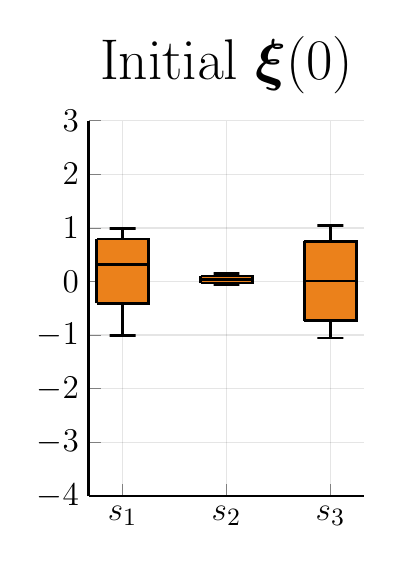
\begin{tikzpicture}[]
\begin{axis}[height = {63.5mm}, ylabel = {}, title = {Initial $\bm \xi(0)$}, xmin = {0.175}, xmax = {2.825}, ymax = {3}, xlabel = {}, unbounded coords=jump,scaled x ticks = false,xlabel style = {font = {\fontsize{18 pt}{23.400000000000002 pt}\selectfont}, color = {rgb,1:red,0.00000000;green,0.00000000;blue,0.00000000}, draw opacity = 1.0, rotate = 0.0},xmajorgrids = true,xtick = {0.5,1.5,2.5},xticklabels = {$s_1$,$s_2$,$s_3$},xtick align = inside,xticklabel style = {font = {\fontsize{13 pt}{16.900000000000002 pt}\selectfont}, color = {rgb,1:red,0.00000000;green,0.00000000;blue,0.00000000}, draw opacity = 1.0, rotate = 0.0},x grid style = {color = {rgb,1:red,0.00000000;green,0.00000000;blue,0.00000000},
draw opacity = 0.1,
line width = 0.5,
solid},axis x line* = left,x axis line style = {color = {rgb,1:red,0.00000000;green,0.00000000;blue,0.00000000},
draw opacity = 1.0,
line width = 1,
solid},scaled y ticks = false,ylabel style = {font = {\fontsize{18 pt}{23.400000000000002 pt}\selectfont}, color = {rgb,1:red,0.00000000;green,0.00000000;blue,0.00000000}, draw opacity = 1.0, rotate = 0.0},ymajorgrids = true,ytick = {-4.0,-3.0,-2.0,-1.0,0.0,1.0,2.0,3.0},yticklabels = {$-4$,$-3$,$-2$,$-1$,$0$,$1$,$2$,$3$},ytick align = inside,yticklabel style = {font = {\fontsize{13 pt}{16.900000000000002 pt}\selectfont}, color = {rgb,1:red,0.00000000;green,0.00000000;blue,0.00000000}, draw opacity = 1.0, rotate = 0.0},y grid style = {color = {rgb,1:red,0.00000000;green,0.00000000;blue,0.00000000},
draw opacity = 0.1,
line width = 0.5,
solid},axis y line* = left,y axis line style = {color = {rgb,1:red,0.00000000;green,0.00000000;blue,0.00000000},
draw opacity = 1.0,
line width = 1,
solid},    xshift = 0.0mm,
    yshift = 0.0mm,
    axis background/.style={fill={rgb,1:red,1.00000000;green,1.00000000;blue,1.00000000}}
,title style = {font = {\fontsize{22 pt}{28.6 pt}\selectfont}, color = {rgb,1:red,0.00000000;green,0.00000000;blue,0.00000000}, draw opacity = 1.0, rotate = 0.0},legend style = {color = {rgb,1:red,0.00000000;green,0.00000000;blue,0.00000000},
draw opacity = 1.0,
line width = 1,
solid,fill = {rgb,1:red,1.00000000;green,1.00000000;blue,1.00000000},font = {\fontsize{13 pt}{16.900000000000002 pt}\selectfont}},colorbar style={title=}, ymin = {-4}, width = {50.8mm}]\addplot+ [color = {rgb,1:red,0.00000000;green,0.00000000;blue,0.00000000},
draw opacity = 1.0,
line width = 1,
solid,mark = none,
mark size = 2.0,
mark options = {
    color = {rgb,1:red,0.00000000;green,0.00000000;blue,0.00000000}, draw opacity = 1.0,
    fill = {rgb,1:red,0.92156863;green,0.50588235;blue,0.10588235}, fill opacity = 1.0,
    line width = 1,
    rotate = 0,
    solid
},fill = {rgb,1:red,0.92156863;green,0.50588235;blue,0.10588235}, fill opacity=1.0,forget plot]coordinates {
(0.5, -1.0093852281570435)
(0.375, -1.0093852281570435)
(0.625, -1.0093852281570435)
(0.5, -1.0093852281570435)
(0.5, -0.4064389243721962)
};
\addplot+ [color = {rgb,1:red,0.00000000;green,0.00000000;blue,0.00000000},
draw opacity = 1.0,
line width = 1,
solid,mark = none,
mark size = 2.0,
mark options = {
    color = {rgb,1:red,0.00000000;green,0.00000000;blue,0.00000000}, draw opacity = 1.0,
    fill = {rgb,1:red,0.92156863;green,0.50588235;blue,0.10588235}, fill opacity = 1.0,
    line width = 1,
    rotate = 0,
    solid
},fill = {rgb,1:red,0.92156863;green,0.50588235;blue,0.10588235}, fill opacity=1.0,forget plot]coordinates {
(0.25, -0.4064389243721962)
(0.25, 0.3174552619457245)
(0.75, 0.3174552619457245)
(0.75, -0.4064389243721962)
(0.25, -0.4064389243721962)
};
\addplot+ [color = {rgb,1:red,0.00000000;green,0.00000000;blue,0.00000000},
draw opacity = 1.0,
line width = 1,
solid,mark = none,
mark size = 2.0,
mark options = {
    color = {rgb,1:red,0.00000000;green,0.00000000;blue,0.00000000}, draw opacity = 1.0,
    fill = {rgb,1:red,0.92156863;green,0.50588235;blue,0.10588235}, fill opacity = 1.0,
    line width = 1,
    rotate = 0,
    solid
},fill = {rgb,1:red,0.92156863;green,0.50588235;blue,0.10588235}, fill opacity=1.0,forget plot]coordinates {
(0.25, 0.7902185618877411)
(0.25, 0.3174552619457245)
(0.75, 0.3174552619457245)
(0.75, 0.7902185618877411)
(0.25, 0.7902185618877411)
};
\addplot+ [color = {rgb,1:red,0.00000000;green,0.00000000;blue,0.00000000},
draw opacity = 1.0,
line width = 1,
solid,mark = none,
mark size = 2.0,
mark options = {
    color = {rgb,1:red,0.00000000;green,0.00000000;blue,0.00000000}, draw opacity = 1.0,
    fill = {rgb,1:red,0.92156863;green,0.50588235;blue,0.10588235}, fill opacity = 1.0,
    line width = 1,
    rotate = 0,
    solid
},fill = {rgb,1:red,0.92156863;green,0.50588235;blue,0.10588235}, fill opacity=1.0,forget plot]coordinates {
(0.5, 0.9865884780883789)
(0.375, 0.9865884780883789)
(0.625, 0.9865884780883789)
(0.5, 0.9865884780883789)
(0.5, 0.7902185618877411)
};
\addplot+ [color = {rgb,1:red,0.00000000;green,0.00000000;blue,0.00000000},
draw opacity = 1.0,
line width = 1,
solid,mark = none,
mark size = 2.0,
mark options = {
    color = {rgb,1:red,0.00000000;green,0.00000000;blue,0.00000000}, draw opacity = 1.0,
    fill = {rgb,1:red,0.92156863;green,0.50588235;blue,0.10588235}, fill opacity = 1.0,
    line width = 1,
    rotate = 0,
    solid
},fill = {rgb,1:red,0.92156863;green,0.50588235;blue,0.10588235}, fill opacity=1.0,forget plot]coordinates {
(1.5, -0.06516765803098679)
(1.375, -0.06516765803098679)
(1.625, -0.06516765803098679)
(1.5, -0.06516765803098679)
(1.5, -0.028776861261576414)
};
\addplot+ [color = {rgb,1:red,0.00000000;green,0.00000000;blue,0.00000000},
draw opacity = 1.0,
line width = 1,
solid,mark = none,
mark size = 2.0,
mark options = {
    color = {rgb,1:red,0.00000000;green,0.00000000;blue,0.00000000}, draw opacity = 1.0,
    fill = {rgb,1:red,0.92156863;green,0.50588235;blue,0.10588235}, fill opacity = 1.0,
    line width = 1,
    rotate = 0,
    solid
},fill = {rgb,1:red,0.92156863;green,0.50588235;blue,0.10588235}, fill opacity=1.0,forget plot]coordinates {
(1.25, -0.028776861261576414)
(1.25, 0.03745450638234615)
(1.75, 0.03745450638234615)
(1.75, -0.028776861261576414)
(1.25, -0.028776861261576414)
};
\addplot+ [color = {rgb,1:red,0.00000000;green,0.00000000;blue,0.00000000},
draw opacity = 1.0,
line width = 1,
solid,mark = none,
mark size = 2.0,
mark options = {
    color = {rgb,1:red,0.00000000;green,0.00000000;blue,0.00000000}, draw opacity = 1.0,
    fill = {rgb,1:red,0.92156863;green,0.50588235;blue,0.10588235}, fill opacity = 1.0,
    line width = 1,
    rotate = 0,
    solid
},fill = {rgb,1:red,0.92156863;green,0.50588235;blue,0.10588235}, fill opacity=1.0,forget plot]coordinates {
(1.25, 0.10362245701253414)
(1.25, 0.03745450638234615)
(1.75, 0.03745450638234615)
(1.75, 0.10362245701253414)
(1.25, 0.10362245701253414)
};
\addplot+ [color = {rgb,1:red,0.00000000;green,0.00000000;blue,0.00000000},
draw opacity = 1.0,
line width = 1,
solid,mark = none,
mark size = 2.0,
mark options = {
    color = {rgb,1:red,0.00000000;green,0.00000000;blue,0.00000000}, draw opacity = 1.0,
    fill = {rgb,1:red,0.92156863;green,0.50588235;blue,0.10588235}, fill opacity = 1.0,
    line width = 1,
    rotate = 0,
    solid
},fill = {rgb,1:red,0.92156863;green,0.50588235;blue,0.10588235}, fill opacity=1.0,forget plot]coordinates {
(1.5, 0.1513187438249588)
(1.375, 0.1513187438249588)
(1.625, 0.1513187438249588)
(1.5, 0.1513187438249588)
(1.5, 0.10362245701253414)
};
\addplot+ [color = {rgb,1:red,0.00000000;green,0.00000000;blue,0.00000000},
draw opacity = 1.0,
line width = 1,
solid,mark = none,
mark size = 2.0,
mark options = {
    color = {rgb,1:red,0.00000000;green,0.00000000;blue,0.00000000}, draw opacity = 1.0,
    fill = {rgb,1:red,0.92156863;green,0.50588235;blue,0.10588235}, fill opacity = 1.0,
    line width = 1,
    rotate = 0,
    solid
},fill = {rgb,1:red,0.92156863;green,0.50588235;blue,0.10588235}, fill opacity=1.0,forget plot]coordinates {
(2.5, -1.055550456047058)
(2.375, -1.055550456047058)
(2.625, -1.055550456047058)
(2.5, -1.055550456047058)
(2.5, -0.7337391972541809)
};
\addplot+ [color = {rgb,1:red,0.00000000;green,0.00000000;blue,0.00000000},
draw opacity = 1.0,
line width = 1,
solid,mark = none,
mark size = 2.0,
mark options = {
    color = {rgb,1:red,0.00000000;green,0.00000000;blue,0.00000000}, draw opacity = 1.0,
    fill = {rgb,1:red,0.92156863;green,0.50588235;blue,0.10588235}, fill opacity = 1.0,
    line width = 1,
    rotate = 0,
    solid
},fill = {rgb,1:red,0.92156863;green,0.50588235;blue,0.10588235}, fill opacity=1.0,forget plot]coordinates {
(2.25, -0.7337391972541809)
(2.25, 0.007332766428589821)
(2.75, 0.007332766428589821)
(2.75, -0.7337391972541809)
(2.25, -0.7337391972541809)
};
\addplot+ [color = {rgb,1:red,0.00000000;green,0.00000000;blue,0.00000000},
draw opacity = 1.0,
line width = 1,
solid,mark = none,
mark size = 2.0,
mark options = {
    color = {rgb,1:red,0.00000000;green,0.00000000;blue,0.00000000}, draw opacity = 1.0,
    fill = {rgb,1:red,0.92156863;green,0.50588235;blue,0.10588235}, fill opacity = 1.0,
    line width = 1,
    rotate = 0,
    solid
},fill = {rgb,1:red,0.92156863;green,0.50588235;blue,0.10588235}, fill opacity=1.0,forget plot]coordinates {
(2.25, 0.7472901940345764)
(2.25, 0.007332766428589821)
(2.75, 0.007332766428589821)
(2.75, 0.7472901940345764)
(2.25, 0.7472901940345764)
};
\addplot+ [color = {rgb,1:red,0.00000000;green,0.00000000;blue,0.00000000},
draw opacity = 1.0,
line width = 1,
solid,mark = none,
mark size = 2.0,
mark options = {
    color = {rgb,1:red,0.00000000;green,0.00000000;blue,0.00000000}, draw opacity = 1.0,
    fill = {rgb,1:red,0.92156863;green,0.50588235;blue,0.10588235}, fill opacity = 1.0,
    line width = 1,
    rotate = 0,
    solid
},fill = {rgb,1:red,0.92156863;green,0.50588235;blue,0.10588235}, fill opacity=1.0,forget plot]coordinates {
(2.5, 1.0507506132125854)
(2.375, 1.0507506132125854)
(2.625, 1.0507506132125854)
(2.5, 1.0507506132125854)
(2.5, 0.7472901940345764)
};
\end{axis}

\end{tikzpicture}
}
  \resizebox{!}{.28\linewidth}{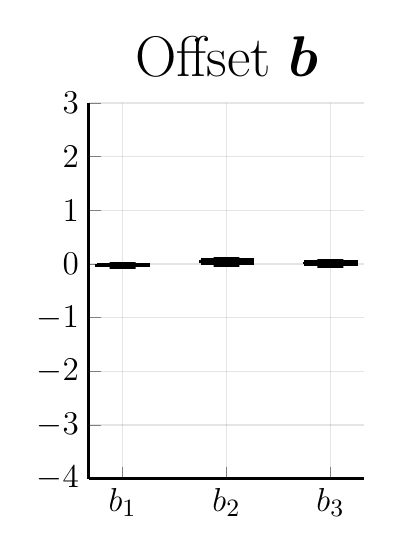
\begin{tikzpicture}[]
\begin{axis}[height = {63.5mm}, ylabel = {}, title = {Offset $\bm b$}, xmin = {0.175}, xmax = {2.825}, ymax = {3}, xlabel = {}, unbounded coords=jump,scaled x ticks = false,xlabel style = {font = {\fontsize{18 pt}{23.400000000000002 pt}\selectfont}, color = {rgb,1:red,0.00000000;green,0.00000000;blue,0.00000000}, draw opacity = 1.0, rotate = 0.0},xmajorgrids = true,xtick = {0.5,1.5,2.5},xticklabels = {$b_1$,$b_2$,$b_3$},xtick align = inside,xticklabel style = {font = {\fontsize{13 pt}{16.900000000000002 pt}\selectfont}, color = {rgb,1:red,0.00000000;green,0.00000000;blue,0.00000000}, draw opacity = 1.0, rotate = 0.0},x grid style = {color = {rgb,1:red,0.00000000;green,0.00000000;blue,0.00000000},
draw opacity = 0.1,
line width = 0.5,
solid},axis x line* = left,x axis line style = {color = {rgb,1:red,0.00000000;green,0.00000000;blue,0.00000000},
draw opacity = 1.0,
line width = 1,
solid},scaled y ticks = false,ylabel style = {font = {\fontsize{18 pt}{23.400000000000002 pt}\selectfont}, color = {rgb,1:red,0.00000000;green,0.00000000;blue,0.00000000}, draw opacity = 1.0, rotate = 0.0},ymajorgrids = true,ytick = {-4.0,-3.0,-2.0,-1.0,0.0,1.0,2.0,3.0},yticklabels = {$-4$,$-3$,$-2$,$-1$,$0$,$1$,$2$,$3$},ytick align = inside,yticklabel style = {font = {\fontsize{13 pt}{16.900000000000002 pt}\selectfont}, color = {rgb,1:red,0.00000000;green,0.00000000;blue,0.00000000}, draw opacity = 1.0, rotate = 0.0},y grid style = {color = {rgb,1:red,0.00000000;green,0.00000000;blue,0.00000000},
draw opacity = 0.1,
line width = 0.5,
solid},axis y line* = left,y axis line style = {color = {rgb,1:red,0.00000000;green,0.00000000;blue,0.00000000},
draw opacity = 1.0,
line width = 1,
solid},    xshift = 0.0mm,
    yshift = 0.0mm,
    axis background/.style={fill={rgb,1:red,1.00000000;green,1.00000000;blue,1.00000000}}
,title style = {font = {\fontsize{22 pt}{28.6 pt}\selectfont}, color = {rgb,1:red,0.00000000;green,0.00000000;blue,0.00000000}, draw opacity = 1.0, rotate = 0.0},legend style = {color = {rgb,1:red,0.00000000;green,0.00000000;blue,0.00000000},
draw opacity = 1.0,
line width = 1,
solid,fill = {rgb,1:red,1.00000000;green,1.00000000;blue,1.00000000},font = {\fontsize{13 pt}{16.900000000000002 pt}\selectfont}},colorbar style={title=}, ymin = {-4}, width = {50.8mm}]\addplot+ [color = {rgb,1:red,0.00000000;green,0.00000000;blue,0.00000000},
draw opacity = 1.0,
line width = 1,
solid,mark = none,
mark size = 2.0,
mark options = {
    color = {rgb,1:red,0.00000000;green,0.00000000;blue,0.00000000}, draw opacity = 1.0,
    fill = {rgb,1:red,0.92156863;green,0.50588235;blue,0.10588235}, fill opacity = 1.0,
    line width = 1,
    rotate = 0,
    solid
},fill = {rgb,1:red,0.92156863;green,0.50588235;blue,0.10588235}, fill opacity=1.0,forget plot]coordinates {
(0.5, -0.07128085196018219)
(0.375, -0.07128085196018219)
(0.625, -0.07128085196018219)
(0.5, -0.07128085196018219)
(0.5, -0.03508143872022629)
};
\addplot+ [color = {rgb,1:red,0.00000000;green,0.00000000;blue,0.00000000},
draw opacity = 1.0,
line width = 1,
solid,mark = none,
mark size = 2.0,
mark options = {
    color = {rgb,1:red,0.00000000;green,0.00000000;blue,0.00000000}, draw opacity = 1.0,
    fill = {rgb,1:red,0.92156863;green,0.50588235;blue,0.10588235}, fill opacity = 1.0,
    line width = 1,
    rotate = 0,
    solid
},fill = {rgb,1:red,0.92156863;green,0.50588235;blue,0.10588235}, fill opacity=1.0,forget plot]coordinates {
(0.25, -0.03508143872022629)
(0.25, -0.023331661708652973)
(0.75, -0.023331661708652973)
(0.75, -0.03508143872022629)
(0.25, -0.03508143872022629)
};
\addplot+ [color = {rgb,1:red,0.00000000;green,0.00000000;blue,0.00000000},
draw opacity = 1.0,
line width = 1,
solid,mark = none,
mark size = 2.0,
mark options = {
    color = {rgb,1:red,0.00000000;green,0.00000000;blue,0.00000000}, draw opacity = 1.0,
    fill = {rgb,1:red,0.92156863;green,0.50588235;blue,0.10588235}, fill opacity = 1.0,
    line width = 1,
    rotate = 0,
    solid
},fill = {rgb,1:red,0.92156863;green,0.50588235;blue,0.10588235}, fill opacity=1.0,forget plot]coordinates {
(0.25, -0.01039293222129345)
(0.25, -0.023331661708652973)
(0.75, -0.023331661708652973)
(0.75, -0.01039293222129345)
(0.25, -0.01039293222129345)
};
\addplot+ [color = {rgb,1:red,0.00000000;green,0.00000000;blue,0.00000000},
draw opacity = 1.0,
line width = 1,
solid,mark = none,
mark size = 2.0,
mark options = {
    color = {rgb,1:red,0.00000000;green,0.00000000;blue,0.00000000}, draw opacity = 1.0,
    fill = {rgb,1:red,0.92156863;green,0.50588235;blue,0.10588235}, fill opacity = 1.0,
    line width = 1,
    rotate = 0,
    solid
},fill = {rgb,1:red,0.92156863;green,0.50588235;blue,0.10588235}, fill opacity=1.0,forget plot]coordinates {
(0.5, 0.019218027591705322)
(0.375, 0.019218027591705322)
(0.625, 0.019218027591705322)
(0.5, 0.019218027591705322)
(0.5, -0.01039293222129345)
};
\addplot+ [color = {rgb,1:red,0.00000000;green,0.00000000;blue,0.00000000},
draw opacity = 1.0,
line width = 1,
solid,mark = none,
mark size = 2.0,
mark options = {
    color = {rgb,1:red,0.00000000;green,0.00000000;blue,0.00000000}, draw opacity = 1.0,
    fill = {rgb,1:red,0.92156863;green,0.50588235;blue,0.10588235}, fill opacity = 1.0,
    line width = 1,
    rotate = 0,
    solid
},fill = {rgb,1:red,0.92156863;green,0.50588235;blue,0.10588235}, fill opacity=1.0,forget plot]coordinates {
(1.5, -0.020190563052892685)
(1.375, -0.020190563052892685)
(1.625, -0.020190563052892685)
(1.5, -0.020190563052892685)
(1.5, 0.011186720803380013)
};
\addplot+ [color = {rgb,1:red,0.00000000;green,0.00000000;blue,0.00000000},
draw opacity = 1.0,
line width = 1,
solid,mark = none,
mark size = 2.0,
mark options = {
    color = {rgb,1:red,0.00000000;green,0.00000000;blue,0.00000000}, draw opacity = 1.0,
    fill = {rgb,1:red,0.92156863;green,0.50588235;blue,0.10588235}, fill opacity = 1.0,
    line width = 1,
    rotate = 0,
    solid
},fill = {rgb,1:red,0.92156863;green,0.50588235;blue,0.10588235}, fill opacity=1.0,forget plot]coordinates {
(1.25, 0.011186720803380013)
(1.25, 0.04952448979020119)
(1.75, 0.04952448979020119)
(1.75, 0.011186720803380013)
(1.25, 0.011186720803380013)
};
\addplot+ [color = {rgb,1:red,0.00000000;green,0.00000000;blue,0.00000000},
draw opacity = 1.0,
line width = 1,
solid,mark = none,
mark size = 2.0,
mark options = {
    color = {rgb,1:red,0.00000000;green,0.00000000;blue,0.00000000}, draw opacity = 1.0,
    fill = {rgb,1:red,0.92156863;green,0.50588235;blue,0.10588235}, fill opacity = 1.0,
    line width = 1,
    rotate = 0,
    solid
},fill = {rgb,1:red,0.92156863;green,0.50588235;blue,0.10588235}, fill opacity=1.0,forget plot]coordinates {
(1.25, 0.08388775587081909)
(1.25, 0.04952448979020119)
(1.75, 0.04952448979020119)
(1.75, 0.08388775587081909)
(1.25, 0.08388775587081909)
};
\addplot+ [color = {rgb,1:red,0.00000000;green,0.00000000;blue,0.00000000},
draw opacity = 1.0,
line width = 1,
solid,mark = none,
mark size = 2.0,
mark options = {
    color = {rgb,1:red,0.00000000;green,0.00000000;blue,0.00000000}, draw opacity = 1.0,
    fill = {rgb,1:red,0.92156863;green,0.50588235;blue,0.10588235}, fill opacity = 1.0,
    line width = 1,
    rotate = 0,
    solid
},fill = {rgb,1:red,0.92156863;green,0.50588235;blue,0.10588235}, fill opacity=1.0,forget plot]coordinates {
(1.5, 0.10372693836688995)
(1.375, 0.10372693836688995)
(1.625, 0.10372693836688995)
(1.5, 0.10372693836688995)
(1.5, 0.08388775587081909)
};
\addplot+ [color = {rgb,1:red,0.00000000;green,0.00000000;blue,0.00000000},
draw opacity = 1.0,
line width = 1,
solid,mark = none,
mark size = 2.0,
mark options = {
    color = {rgb,1:red,0.00000000;green,0.00000000;blue,0.00000000}, draw opacity = 1.0,
    fill = {rgb,1:red,0.92156863;green,0.50588235;blue,0.10588235}, fill opacity = 1.0,
    line width = 1,
    rotate = 0,
    solid
},fill = {rgb,1:red,0.92156863;green,0.50588235;blue,0.10588235}, fill opacity=1.0,forget plot]coordinates {
(2.5, -0.04140687361359596)
(2.375, -0.04140687361359596)
(2.625, -0.04140687361359596)
(2.5, -0.04140687361359596)
(2.5, -0.006251898128539324)
};
\addplot+ [color = {rgb,1:red,0.00000000;green,0.00000000;blue,0.00000000},
draw opacity = 1.0,
line width = 1,
solid,mark = none,
mark size = 2.0,
mark options = {
    color = {rgb,1:red,0.00000000;green,0.00000000;blue,0.00000000}, draw opacity = 1.0,
    fill = {rgb,1:red,0.92156863;green,0.50588235;blue,0.10588235}, fill opacity = 1.0,
    line width = 1,
    rotate = 0,
    solid
},fill = {rgb,1:red,0.92156863;green,0.50588235;blue,0.10588235}, fill opacity=1.0,forget plot]coordinates {
(2.25, -0.006251898128539324)
(2.25, 0.02104303054511547)
(2.75, 0.02104303054511547)
(2.75, -0.006251898128539324)
(2.25, -0.006251898128539324)
};
\addplot+ [color = {rgb,1:red,0.00000000;green,0.00000000;blue,0.00000000},
draw opacity = 1.0,
line width = 1,
solid,mark = none,
mark size = 2.0,
mark options = {
    color = {rgb,1:red,0.00000000;green,0.00000000;blue,0.00000000}, draw opacity = 1.0,
    fill = {rgb,1:red,0.92156863;green,0.50588235;blue,0.10588235}, fill opacity = 1.0,
    line width = 1,
    rotate = 0,
    solid
},fill = {rgb,1:red,0.92156863;green,0.50588235;blue,0.10588235}, fill opacity=1.0,forget plot]coordinates {
(2.25, 0.041737623512744904)
(2.25, 0.02104303054511547)
(2.75, 0.02104303054511547)
(2.75, 0.041737623512744904)
(2.25, 0.041737623512744904)
};
\addplot+ [color = {rgb,1:red,0.00000000;green,0.00000000;blue,0.00000000},
draw opacity = 1.0,
line width = 1,
solid,mark = none,
mark size = 2.0,
mark options = {
    color = {rgb,1:red,0.00000000;green,0.00000000;blue,0.00000000}, draw opacity = 1.0,
    fill = {rgb,1:red,0.92156863;green,0.50588235;blue,0.10588235}, fill opacity = 1.0,
    line width = 1,
    rotate = 0,
    solid
},fill = {rgb,1:red,0.92156863;green,0.50588235;blue,0.10588235}, fill opacity=1.0,forget plot]coordinates {
(2.5, 0.07456278800964355)
(2.375, 0.07456278800964355)
(2.625, 0.07456278800964355)
(2.5, 0.07456278800964355)
(2.5, 0.041737623512744904)
};
\end{axis}

\end{tikzpicture}
}

  \resizebox{!}{.28\linewidth}{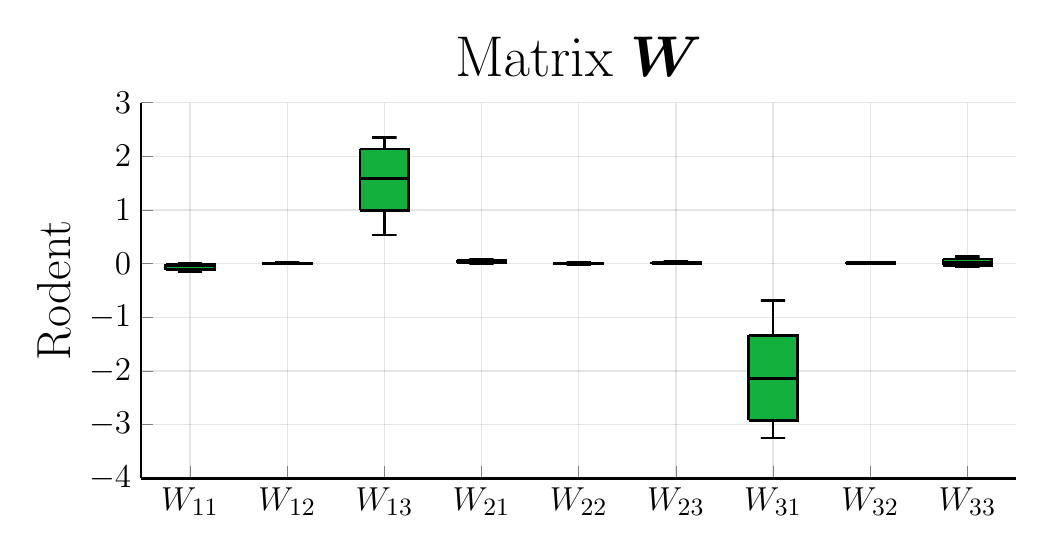
\begin{tikzpicture}[]
\begin{axis}[height = {63.5mm}, ylabel = {Rodent}, title = {Matrix $\bm W$}, xmin = {-0.0050000000000000044}, xmax = {9.005}, ymax = {3}, xlabel = {}, unbounded coords=jump,scaled x ticks = false,xlabel style = {font = {\fontsize{18 pt}{23.400000000000002 pt}\selectfont}, color = {rgb,1:red,0.00000000;green,0.00000000;blue,0.00000000}, draw opacity = 1.0, rotate = 0.0},xmajorgrids = true,xtick = {0.5,1.5,2.5,3.5,4.5,5.5,6.5,7.5,8.5},xticklabels = {$W_{11}$,$W_{12}$,$W_{13}$,$W_{21}$,$W_{22}$,$W_{23}$,$W_{31}$,$W_{32}$,$W_{33}$},xtick align = inside,xticklabel style = {font = {\fontsize{13 pt}{16.900000000000002 pt}\selectfont}, color = {rgb,1:red,0.00000000;green,0.00000000;blue,0.00000000}, draw opacity = 1.0, rotate = 0.0},x grid style = {color = {rgb,1:red,0.00000000;green,0.00000000;blue,0.00000000},
draw opacity = 0.1,
line width = 0.5,
solid},axis x line* = left,x axis line style = {color = {rgb,1:red,0.00000000;green,0.00000000;blue,0.00000000},
draw opacity = 1.0,
line width = 1,
solid},scaled y ticks = false,ylabel style = {font = {\fontsize{18 pt}{23.400000000000002 pt}\selectfont}, color = {rgb,1:red,0.00000000;green,0.00000000;blue,0.00000000}, draw opacity = 1.0, rotate = 0.0},ymajorgrids = true,ytick = {-4.0,-3.0,-2.0,-1.0,0.0,1.0,2.0,3.0},yticklabels = {$-4$,$-3$,$-2$,$-1$,$0$,$1$,$2$,$3$},ytick align = inside,yticklabel style = {font = {\fontsize{13 pt}{16.900000000000002 pt}\selectfont}, color = {rgb,1:red,0.00000000;green,0.00000000;blue,0.00000000}, draw opacity = 1.0, rotate = 0.0},y grid style = {color = {rgb,1:red,0.00000000;green,0.00000000;blue,0.00000000},
draw opacity = 0.1,
line width = 0.5,
solid},axis y line* = left,y axis line style = {color = {rgb,1:red,0.00000000;green,0.00000000;blue,0.00000000},
draw opacity = 1.0,
line width = 1,
solid},    xshift = 0.0mm,
    yshift = 0.0mm,
    axis background/.style={fill={rgb,1:red,1.00000000;green,1.00000000;blue,1.00000000}}
,title style = {font = {\fontsize{22 pt}{28.6 pt}\selectfont}, color = {rgb,1:red,0.00000000;green,0.00000000;blue,0.00000000}, draw opacity = 1.0, rotate = 0.0},legend style = {color = {rgb,1:red,0.00000000;green,0.00000000;blue,0.00000000},
draw opacity = 1.0,
line width = 1,
solid,fill = {rgb,1:red,1.00000000;green,1.00000000;blue,1.00000000},font = {\fontsize{13 pt}{16.900000000000002 pt}\selectfont}},colorbar style={title=}, ymin = {-4}, width = {127.0mm}]\addplot+ [color = {rgb,1:red,0.00000000;green,0.00000000;blue,0.00000000},
draw opacity = 1.0,
line width = 1,
solid,mark = none,
mark size = 2.0,
mark options = {
    color = {rgb,1:red,0.00000000;green,0.00000000;blue,0.00000000}, draw opacity = 1.0,
    fill = {rgb,1:red,0.07843137;green,0.69019608;blue,0.23921569}, fill opacity = 1.0,
    line width = 1,
    rotate = 0,
    solid
},fill = {rgb,1:red,0.07843137;green,0.69019608;blue,0.23921569}, fill opacity=1.0,forget plot]coordinates {
(0.5, -0.15230727195739746)
(0.375, -0.15230727195739746)
(0.625, -0.15230727195739746)
(0.5, -0.15230727195739746)
(0.5, -0.11162257753312588)
};
\addplot+ [color = {rgb,1:red,0.00000000;green,0.00000000;blue,0.00000000},
draw opacity = 1.0,
line width = 1,
solid,mark = none,
mark size = 2.0,
mark options = {
    color = {rgb,1:red,0.00000000;green,0.00000000;blue,0.00000000}, draw opacity = 1.0,
    fill = {rgb,1:red,0.07843137;green,0.69019608;blue,0.23921569}, fill opacity = 1.0,
    line width = 1,
    rotate = 0,
    solid
},fill = {rgb,1:red,0.07843137;green,0.69019608;blue,0.23921569}, fill opacity=1.0,forget plot]coordinates {
(0.25, -0.11162257753312588)
(0.25, -0.039449092000722885)
(0.75, -0.039449092000722885)
(0.75, -0.11162257753312588)
(0.25, -0.11162257753312588)
};
\addplot+ [color = {rgb,1:red,0.00000000;green,0.00000000;blue,0.00000000},
draw opacity = 1.0,
line width = 1,
solid,mark = none,
mark size = 2.0,
mark options = {
    color = {rgb,1:red,0.00000000;green,0.00000000;blue,0.00000000}, draw opacity = 1.0,
    fill = {rgb,1:red,0.07843137;green,0.69019608;blue,0.23921569}, fill opacity = 1.0,
    line width = 1,
    rotate = 0,
    solid
},fill = {rgb,1:red,0.07843137;green,0.69019608;blue,0.23921569}, fill opacity=1.0,forget plot]coordinates {
(0.25, -0.008502990007400513)
(0.25, -0.039449092000722885)
(0.75, -0.039449092000722885)
(0.75, -0.008502990007400513)
(0.25, -0.008502990007400513)
};
\addplot+ [color = {rgb,1:red,0.00000000;green,0.00000000;blue,0.00000000},
draw opacity = 1.0,
line width = 1,
solid,mark = none,
mark size = 2.0,
mark options = {
    color = {rgb,1:red,0.00000000;green,0.00000000;blue,0.00000000}, draw opacity = 1.0,
    fill = {rgb,1:red,0.07843137;green,0.69019608;blue,0.23921569}, fill opacity = 1.0,
    line width = 1,
    rotate = 0,
    solid
},fill = {rgb,1:red,0.07843137;green,0.69019608;blue,0.23921569}, fill opacity=1.0,forget plot]coordinates {
(0.5, 0.0059748440980911255)
(0.375, 0.0059748440980911255)
(0.625, 0.0059748440980911255)
(0.5, 0.0059748440980911255)
(0.5, -0.008502990007400513)
};
\addplot+ [color = {rgb,1:red,0.00000000;green,0.00000000;blue,0.00000000},
draw opacity = 1.0,
line width = 1,
solid,mark = none,
mark size = 2.0,
mark options = {
    color = {rgb,1:red,0.00000000;green,0.00000000;blue,0.00000000}, draw opacity = 1.0,
    fill = {rgb,1:red,0.07843137;green,0.69019608;blue,0.23921569}, fill opacity = 1.0,
    line width = 1,
    rotate = 0,
    solid
},fill = {rgb,1:red,0.07843137;green,0.69019608;blue,0.23921569}, fill opacity=1.0,forget plot]coordinates {
(1.5, -0.006154850125312805)
(1.375, -0.006154850125312805)
(1.625, -0.006154850125312805)
(1.5, -0.006154850125312805)
(1.5, -0.0026893513277173042)
};
\addplot+ [color = {rgb,1:red,0.00000000;green,0.00000000;blue,0.00000000},
draw opacity = 1.0,
line width = 1,
solid,mark = none,
mark size = 2.0,
mark options = {
    color = {rgb,1:red,0.00000000;green,0.00000000;blue,0.00000000}, draw opacity = 1.0,
    fill = {rgb,1:red,0.07843137;green,0.69019608;blue,0.23921569}, fill opacity = 1.0,
    line width = 1,
    rotate = 0,
    solid
},fill = {rgb,1:red,0.07843137;green,0.69019608;blue,0.23921569}, fill opacity=1.0,forget plot]coordinates {
(1.25, -0.0026893513277173042)
(1.25, 0.0004074741154909134)
(1.75, 0.0004074741154909134)
(1.75, -0.0026893513277173042)
(1.25, -0.0026893513277173042)
};
\addplot+ [color = {rgb,1:red,0.00000000;green,0.00000000;blue,0.00000000},
draw opacity = 1.0,
line width = 1,
solid,mark = none,
mark size = 2.0,
mark options = {
    color = {rgb,1:red,0.00000000;green,0.00000000;blue,0.00000000}, draw opacity = 1.0,
    fill = {rgb,1:red,0.07843137;green,0.69019608;blue,0.23921569}, fill opacity = 1.0,
    line width = 1,
    rotate = 0,
    solid
},fill = {rgb,1:red,0.07843137;green,0.69019608;blue,0.23921569}, fill opacity=1.0,forget plot]coordinates {
(1.25, 0.009917276445776224)
(1.25, 0.0004074741154909134)
(1.75, 0.0004074741154909134)
(1.75, 0.009917276445776224)
(1.25, 0.009917276445776224)
};
\addplot+ [color = {rgb,1:red,0.00000000;green,0.00000000;blue,0.00000000},
draw opacity = 1.0,
line width = 1,
solid,mark = none,
mark size = 2.0,
mark options = {
    color = {rgb,1:red,0.00000000;green,0.00000000;blue,0.00000000}, draw opacity = 1.0,
    fill = {rgb,1:red,0.07843137;green,0.69019608;blue,0.23921569}, fill opacity = 1.0,
    line width = 1,
    rotate = 0,
    solid
},fill = {rgb,1:red,0.07843137;green,0.69019608;blue,0.23921569}, fill opacity=1.0,forget plot]coordinates {
(1.5, 0.028402179479599)
(1.375, 0.028402179479599)
(1.625, 0.028402179479599)
(1.5, 0.028402179479599)
(1.5, 0.009917276445776224)
};
\addplot+ [color = {rgb,1:red,0.00000000;green,0.00000000;blue,0.00000000},
draw opacity = 1.0,
line width = 1,
solid,mark = none,
mark size = 2.0,
mark options = {
    color = {rgb,1:red,0.00000000;green,0.00000000;blue,0.00000000}, draw opacity = 1.0,
    fill = {rgb,1:red,0.07843137;green,0.69019608;blue,0.23921569}, fill opacity = 1.0,
    line width = 1,
    rotate = 0,
    solid
},fill = {rgb,1:red,0.07843137;green,0.69019608;blue,0.23921569}, fill opacity=1.0,forget plot]coordinates {
(2.5, 0.5319146513938904)
(2.375, 0.5319146513938904)
(2.625, 0.5319146513938904)
(2.5, 0.5319146513938904)
(2.5, 0.9957987666130066)
};
\addplot+ [color = {rgb,1:red,0.00000000;green,0.00000000;blue,0.00000000},
draw opacity = 1.0,
line width = 1,
solid,mark = none,
mark size = 2.0,
mark options = {
    color = {rgb,1:red,0.00000000;green,0.00000000;blue,0.00000000}, draw opacity = 1.0,
    fill = {rgb,1:red,0.07843137;green,0.69019608;blue,0.23921569}, fill opacity = 1.0,
    line width = 1,
    rotate = 0,
    solid
},fill = {rgb,1:red,0.07843137;green,0.69019608;blue,0.23921569}, fill opacity=1.0,forget plot]coordinates {
(2.25, 0.9957987666130066)
(2.25, 1.592684030532837)
(2.75, 1.592684030532837)
(2.75, 0.9957987666130066)
(2.25, 0.9957987666130066)
};
\addplot+ [color = {rgb,1:red,0.00000000;green,0.00000000;blue,0.00000000},
draw opacity = 1.0,
line width = 1,
solid,mark = none,
mark size = 2.0,
mark options = {
    color = {rgb,1:red,0.00000000;green,0.00000000;blue,0.00000000}, draw opacity = 1.0,
    fill = {rgb,1:red,0.07843137;green,0.69019608;blue,0.23921569}, fill opacity = 1.0,
    line width = 1,
    rotate = 0,
    solid
},fill = {rgb,1:red,0.07843137;green,0.69019608;blue,0.23921569}, fill opacity=1.0,forget plot]coordinates {
(2.25, 2.1376001834869385)
(2.25, 1.592684030532837)
(2.75, 1.592684030532837)
(2.75, 2.1376001834869385)
(2.25, 2.1376001834869385)
};
\addplot+ [color = {rgb,1:red,0.00000000;green,0.00000000;blue,0.00000000},
draw opacity = 1.0,
line width = 1,
solid,mark = none,
mark size = 2.0,
mark options = {
    color = {rgb,1:red,0.00000000;green,0.00000000;blue,0.00000000}, draw opacity = 1.0,
    fill = {rgb,1:red,0.07843137;green,0.69019608;blue,0.23921569}, fill opacity = 1.0,
    line width = 1,
    rotate = 0,
    solid
},fill = {rgb,1:red,0.07843137;green,0.69019608;blue,0.23921569}, fill opacity=1.0,forget plot]coordinates {
(2.5, 2.3552517890930176)
(2.375, 2.3552517890930176)
(2.625, 2.3552517890930176)
(2.5, 2.3552517890930176)
(2.5, 2.1376001834869385)
};
\addplot+ [color = {rgb,1:red,0.00000000;green,0.00000000;blue,0.00000000},
draw opacity = 1.0,
line width = 1,
solid,mark = none,
mark size = 2.0,
mark options = {
    color = {rgb,1:red,0.00000000;green,0.00000000;blue,0.00000000}, draw opacity = 1.0,
    fill = {rgb,1:red,0.07843137;green,0.69019608;blue,0.23921569}, fill opacity = 1.0,
    line width = 1,
    rotate = 0,
    solid
},fill = {rgb,1:red,0.07843137;green,0.69019608;blue,0.23921569}, fill opacity=1.0,forget plot]coordinates {
(3.5, -0.007374929264187813)
(3.375, -0.007374929264187813)
(3.625, -0.007374929264187813)
(3.5, -0.007374929264187813)
(3.5, 0.013446491211652756)
};
\addplot+ [color = {rgb,1:red,0.00000000;green,0.00000000;blue,0.00000000},
draw opacity = 1.0,
line width = 1,
solid,mark = none,
mark size = 2.0,
mark options = {
    color = {rgb,1:red,0.00000000;green,0.00000000;blue,0.00000000}, draw opacity = 1.0,
    fill = {rgb,1:red,0.07843137;green,0.69019608;blue,0.23921569}, fill opacity = 1.0,
    line width = 1,
    rotate = 0,
    solid
},fill = {rgb,1:red,0.07843137;green,0.69019608;blue,0.23921569}, fill opacity=1.0,forget plot]coordinates {
(3.25, 0.013446491211652756)
(3.25, 0.03636573441326618)
(3.75, 0.03636573441326618)
(3.75, 0.013446491211652756)
(3.25, 0.013446491211652756)
};
\addplot+ [color = {rgb,1:red,0.00000000;green,0.00000000;blue,0.00000000},
draw opacity = 1.0,
line width = 1,
solid,mark = none,
mark size = 2.0,
mark options = {
    color = {rgb,1:red,0.00000000;green,0.00000000;blue,0.00000000}, draw opacity = 1.0,
    fill = {rgb,1:red,0.07843137;green,0.69019608;blue,0.23921569}, fill opacity = 1.0,
    line width = 1,
    rotate = 0,
    solid
},fill = {rgb,1:red,0.07843137;green,0.69019608;blue,0.23921569}, fill opacity=1.0,forget plot]coordinates {
(3.25, 0.05548914894461632)
(3.25, 0.03636573441326618)
(3.75, 0.03636573441326618)
(3.75, 0.05548914894461632)
(3.25, 0.05548914894461632)
};
\addplot+ [color = {rgb,1:red,0.00000000;green,0.00000000;blue,0.00000000},
draw opacity = 1.0,
line width = 1,
solid,mark = none,
mark size = 2.0,
mark options = {
    color = {rgb,1:red,0.00000000;green,0.00000000;blue,0.00000000}, draw opacity = 1.0,
    fill = {rgb,1:red,0.07843137;green,0.69019608;blue,0.23921569}, fill opacity = 1.0,
    line width = 1,
    rotate = 0,
    solid
},fill = {rgb,1:red,0.07843137;green,0.69019608;blue,0.23921569}, fill opacity=1.0,forget plot]coordinates {
(3.5, 0.07503050565719604)
(3.375, 0.07503050565719604)
(3.625, 0.07503050565719604)
(3.5, 0.07503050565719604)
(3.5, 0.05548914894461632)
};
\addplot+ [color = {rgb,1:red,0.00000000;green,0.00000000;blue,0.00000000},
draw opacity = 1.0,
line width = 1,
solid,mark = none,
mark size = 2.0,
mark options = {
    color = {rgb,1:red,0.00000000;green,0.00000000;blue,0.00000000}, draw opacity = 1.0,
    fill = {rgb,1:red,0.07843137;green,0.69019608;blue,0.23921569}, fill opacity = 1.0,
    line width = 1,
    rotate = 0,
    solid
},fill = {rgb,1:red,0.07843137;green,0.69019608;blue,0.23921569}, fill opacity=1.0,forget plot]coordinates {
(4.5, -0.01320381835103035)
(4.375, -0.01320381835103035)
(4.625, -0.01320381835103035)
(4.5, -0.01320381835103035)
(4.5, -0.005945350043475628)
};
\addplot+ [color = {rgb,1:red,0.00000000;green,0.00000000;blue,0.00000000},
draw opacity = 1.0,
line width = 1,
solid,mark = none,
mark size = 2.0,
mark options = {
    color = {rgb,1:red,0.00000000;green,0.00000000;blue,0.00000000}, draw opacity = 1.0,
    fill = {rgb,1:red,0.07843137;green,0.69019608;blue,0.23921569}, fill opacity = 1.0,
    line width = 1,
    rotate = 0,
    solid
},fill = {rgb,1:red,0.07843137;green,0.69019608;blue,0.23921569}, fill opacity=1.0,forget plot]coordinates {
(4.25, -0.005945350043475628)
(4.25, -0.0023958534002304077)
(4.75, -0.0023958534002304077)
(4.75, -0.005945350043475628)
(4.25, -0.005945350043475628)
};
\addplot+ [color = {rgb,1:red,0.00000000;green,0.00000000;blue,0.00000000},
draw opacity = 1.0,
line width = 1,
solid,mark = none,
mark size = 2.0,
mark options = {
    color = {rgb,1:red,0.00000000;green,0.00000000;blue,0.00000000}, draw opacity = 1.0,
    fill = {rgb,1:red,0.07843137;green,0.69019608;blue,0.23921569}, fill opacity = 1.0,
    line width = 1,
    rotate = 0,
    solid
},fill = {rgb,1:red,0.07843137;green,0.69019608;blue,0.23921569}, fill opacity=1.0,forget plot]coordinates {
(4.25, 0.0035618217661976814)
(4.25, -0.0023958534002304077)
(4.75, -0.0023958534002304077)
(4.75, 0.0035618217661976814)
(4.25, 0.0035618217661976814)
};
\addplot+ [color = {rgb,1:red,0.00000000;green,0.00000000;blue,0.00000000},
draw opacity = 1.0,
line width = 1,
solid,mark = none,
mark size = 2.0,
mark options = {
    color = {rgb,1:red,0.00000000;green,0.00000000;blue,0.00000000}, draw opacity = 1.0,
    fill = {rgb,1:red,0.07843137;green,0.69019608;blue,0.23921569}, fill opacity = 1.0,
    line width = 1,
    rotate = 0,
    solid
},fill = {rgb,1:red,0.07843137;green,0.69019608;blue,0.23921569}, fill opacity=1.0,forget plot]coordinates {
(4.5, 0.014191884547472)
(4.375, 0.014191884547472)
(4.625, 0.014191884547472)
(4.5, 0.014191884547472)
(4.5, 0.0035618217661976814)
};
\addplot+ [color = {rgb,1:red,0.00000000;green,0.00000000;blue,0.00000000},
draw opacity = 1.0,
line width = 1,
solid,mark = none,
mark size = 2.0,
mark options = {
    color = {rgb,1:red,0.00000000;green,0.00000000;blue,0.00000000}, draw opacity = 1.0,
    fill = {rgb,1:red,0.07843137;green,0.69019608;blue,0.23921569}, fill opacity = 1.0,
    line width = 1,
    rotate = 0,
    solid
},fill = {rgb,1:red,0.07843137;green,0.69019608;blue,0.23921569}, fill opacity=1.0,forget plot]coordinates {
(5.5, -0.0007588313892483711)
(5.375, -0.0007588313892483711)
(5.625, -0.0007588313892483711)
(5.5, -0.0007588313892483711)
(5.5, 0.005735257873311639)
};
\addplot+ [color = {rgb,1:red,0.00000000;green,0.00000000;blue,0.00000000},
draw opacity = 1.0,
line width = 1,
solid,mark = none,
mark size = 2.0,
mark options = {
    color = {rgb,1:red,0.00000000;green,0.00000000;blue,0.00000000}, draw opacity = 1.0,
    fill = {rgb,1:red,0.07843137;green,0.69019608;blue,0.23921569}, fill opacity = 1.0,
    line width = 1,
    rotate = 0,
    solid
},fill = {rgb,1:red,0.07843137;green,0.69019608;blue,0.23921569}, fill opacity=1.0,forget plot]coordinates {
(5.25, 0.005735257873311639)
(5.25, 0.009489579126238823)
(5.75, 0.009489579126238823)
(5.75, 0.005735257873311639)
(5.25, 0.005735257873311639)
};
\addplot+ [color = {rgb,1:red,0.00000000;green,0.00000000;blue,0.00000000},
draw opacity = 1.0,
line width = 1,
solid,mark = none,
mark size = 2.0,
mark options = {
    color = {rgb,1:red,0.00000000;green,0.00000000;blue,0.00000000}, draw opacity = 1.0,
    fill = {rgb,1:red,0.07843137;green,0.69019608;blue,0.23921569}, fill opacity = 1.0,
    line width = 1,
    rotate = 0,
    solid
},fill = {rgb,1:red,0.07843137;green,0.69019608;blue,0.23921569}, fill opacity=1.0,forget plot]coordinates {
(5.25, 0.02724070753902197)
(5.25, 0.009489579126238823)
(5.75, 0.009489579126238823)
(5.75, 0.02724070753902197)
(5.25, 0.02724070753902197)
};
\addplot+ [color = {rgb,1:red,0.00000000;green,0.00000000;blue,0.00000000},
draw opacity = 1.0,
line width = 1,
solid,mark = none,
mark size = 2.0,
mark options = {
    color = {rgb,1:red,0.00000000;green,0.00000000;blue,0.00000000}, draw opacity = 1.0,
    fill = {rgb,1:red,0.07843137;green,0.69019608;blue,0.23921569}, fill opacity = 1.0,
    line width = 1,
    rotate = 0,
    solid
},fill = {rgb,1:red,0.07843137;green,0.69019608;blue,0.23921569}, fill opacity=1.0,forget plot]coordinates {
(5.5, 0.042545512318611145)
(5.375, 0.042545512318611145)
(5.625, 0.042545512318611145)
(5.5, 0.042545512318611145)
(5.5, 0.02724070753902197)
};
\addplot+ [color = {rgb,1:red,0.00000000;green,0.00000000;blue,0.00000000},
draw opacity = 1.0,
line width = 1,
solid,mark = none,
mark size = 2.0,
mark options = {
    color = {rgb,1:red,0.00000000;green,0.00000000;blue,0.00000000}, draw opacity = 1.0,
    fill = {rgb,1:red,0.07843137;green,0.69019608;blue,0.23921569}, fill opacity = 1.0,
    line width = 1,
    rotate = 0,
    solid
},fill = {rgb,1:red,0.07843137;green,0.69019608;blue,0.23921569}, fill opacity=1.0,forget plot]coordinates {
(6.5, -3.251945734024048)
(6.375, -3.251945734024048)
(6.625, -3.251945734024048)
(6.5, -3.251945734024048)
(6.5, -2.924857795238495)
};
\addplot+ [color = {rgb,1:red,0.00000000;green,0.00000000;blue,0.00000000},
draw opacity = 1.0,
line width = 1,
solid,mark = none,
mark size = 2.0,
mark options = {
    color = {rgb,1:red,0.00000000;green,0.00000000;blue,0.00000000}, draw opacity = 1.0,
    fill = {rgb,1:red,0.07843137;green,0.69019608;blue,0.23921569}, fill opacity = 1.0,
    line width = 1,
    rotate = 0,
    solid
},fill = {rgb,1:red,0.07843137;green,0.69019608;blue,0.23921569}, fill opacity=1.0,forget plot]coordinates {
(6.25, -2.924857795238495)
(6.25, -2.147281765937805)
(6.75, -2.147281765937805)
(6.75, -2.924857795238495)
(6.25, -2.924857795238495)
};
\addplot+ [color = {rgb,1:red,0.00000000;green,0.00000000;blue,0.00000000},
draw opacity = 1.0,
line width = 1,
solid,mark = none,
mark size = 2.0,
mark options = {
    color = {rgb,1:red,0.00000000;green,0.00000000;blue,0.00000000}, draw opacity = 1.0,
    fill = {rgb,1:red,0.07843137;green,0.69019608;blue,0.23921569}, fill opacity = 1.0,
    line width = 1,
    rotate = 0,
    solid
},fill = {rgb,1:red,0.07843137;green,0.69019608;blue,0.23921569}, fill opacity=1.0,forget plot]coordinates {
(6.25, -1.3345645070075989)
(6.25, -2.147281765937805)
(6.75, -2.147281765937805)
(6.75, -1.3345645070075989)
(6.25, -1.3345645070075989)
};
\addplot+ [color = {rgb,1:red,0.00000000;green,0.00000000;blue,0.00000000},
draw opacity = 1.0,
line width = 1,
solid,mark = none,
mark size = 2.0,
mark options = {
    color = {rgb,1:red,0.00000000;green,0.00000000;blue,0.00000000}, draw opacity = 1.0,
    fill = {rgb,1:red,0.07843137;green,0.69019608;blue,0.23921569}, fill opacity = 1.0,
    line width = 1,
    rotate = 0,
    solid
},fill = {rgb,1:red,0.07843137;green,0.69019608;blue,0.23921569}, fill opacity=1.0,forget plot]coordinates {
(6.5, -0.6896809339523315)
(6.375, -0.6896809339523315)
(6.625, -0.6896809339523315)
(6.5, -0.6896809339523315)
(6.5, -1.3345645070075989)
};
\addplot+ [color = {rgb,1:red,0.00000000;green,0.00000000;blue,0.00000000},
draw opacity = 1.0,
line width = 1,
solid,mark = none,
mark size = 2.0,
mark options = {
    color = {rgb,1:red,0.00000000;green,0.00000000;blue,0.00000000}, draw opacity = 1.0,
    fill = {rgb,1:red,0.07843137;green,0.69019608;blue,0.23921569}, fill opacity = 1.0,
    line width = 1,
    rotate = 0,
    solid
},fill = {rgb,1:red,0.07843137;green,0.69019608;blue,0.23921569}, fill opacity=1.0,forget plot]coordinates {
(7.5, -0.004452571272850037)
(7.375, -0.004452571272850037)
(7.625, -0.004452571272850037)
(7.5, -0.004452571272850037)
(7.5, 0.005575779941864312)
};
\addplot+ [color = {rgb,1:red,0.00000000;green,0.00000000;blue,0.00000000},
draw opacity = 1.0,
line width = 1,
solid,mark = none,
mark size = 2.0,
mark options = {
    color = {rgb,1:red,0.00000000;green,0.00000000;blue,0.00000000}, draw opacity = 1.0,
    fill = {rgb,1:red,0.07843137;green,0.69019608;blue,0.23921569}, fill opacity = 1.0,
    line width = 1,
    rotate = 0,
    solid
},fill = {rgb,1:red,0.07843137;green,0.69019608;blue,0.23921569}, fill opacity=1.0,forget plot]coordinates {
(7.25, 0.005575779941864312)
(7.25, 0.012050547637045383)
(7.75, 0.012050547637045383)
(7.75, 0.005575779941864312)
(7.25, 0.005575779941864312)
};
\addplot+ [color = {rgb,1:red,0.00000000;green,0.00000000;blue,0.00000000},
draw opacity = 1.0,
line width = 1,
solid,mark = none,
mark size = 2.0,
mark options = {
    color = {rgb,1:red,0.00000000;green,0.00000000;blue,0.00000000}, draw opacity = 1.0,
    fill = {rgb,1:red,0.07843137;green,0.69019608;blue,0.23921569}, fill opacity = 1.0,
    line width = 1,
    rotate = 0,
    solid
},fill = {rgb,1:red,0.07843137;green,0.69019608;blue,0.23921569}, fill opacity=1.0,forget plot]coordinates {
(7.25, 0.016570504754781723)
(7.25, 0.012050547637045383)
(7.75, 0.012050547637045383)
(7.75, 0.016570504754781723)
(7.25, 0.016570504754781723)
};
\addplot+ [color = {rgb,1:red,0.00000000;green,0.00000000;blue,0.00000000},
draw opacity = 1.0,
line width = 1,
solid,mark = none,
mark size = 2.0,
mark options = {
    color = {rgb,1:red,0.00000000;green,0.00000000;blue,0.00000000}, draw opacity = 1.0,
    fill = {rgb,1:red,0.07843137;green,0.69019608;blue,0.23921569}, fill opacity = 1.0,
    line width = 1,
    rotate = 0,
    solid
},fill = {rgb,1:red,0.07843137;green,0.69019608;blue,0.23921569}, fill opacity=1.0,forget plot]coordinates {
(7.5, 0.026397258043289185)
(7.375, 0.026397258043289185)
(7.625, 0.026397258043289185)
(7.5, 0.026397258043289185)
(7.5, 0.016570504754781723)
};
\addplot+ [color = {rgb,1:red,0.00000000;green,0.00000000;blue,0.00000000},
draw opacity = 1.0,
line width = 1,
solid,mark = none,
mark size = 2.0,
mark options = {
    color = {rgb,1:red,0.00000000;green,0.00000000;blue,0.00000000}, draw opacity = 1.0,
    fill = {rgb,1:red,0.07843137;green,0.69019608;blue,0.23921569}, fill opacity = 1.0,
    line width = 1,
    rotate = 0,
    solid
},fill = {rgb,1:red,0.07843137;green,0.69019608;blue,0.23921569}, fill opacity=1.0,forget plot]coordinates {
(8.5, -0.05648396909236908)
(8.375, -0.05648396909236908)
(8.625, -0.05648396909236908)
(8.5, -0.05648396909236908)
(8.5, -0.035443658009171486)
};
\addplot+ [color = {rgb,1:red,0.00000000;green,0.00000000;blue,0.00000000},
draw opacity = 1.0,
line width = 1,
solid,mark = none,
mark size = 2.0,
mark options = {
    color = {rgb,1:red,0.00000000;green,0.00000000;blue,0.00000000}, draw opacity = 1.0,
    fill = {rgb,1:red,0.07843137;green,0.69019608;blue,0.23921569}, fill opacity = 1.0,
    line width = 1,
    rotate = 0,
    solid
},fill = {rgb,1:red,0.07843137;green,0.69019608;blue,0.23921569}, fill opacity=1.0,forget plot]coordinates {
(8.25, -0.035443658009171486)
(8.25, 0.013854816555976868)
(8.75, 0.013854816555976868)
(8.75, -0.035443658009171486)
(8.25, -0.035443658009171486)
};
\addplot+ [color = {rgb,1:red,0.00000000;green,0.00000000;blue,0.00000000},
draw opacity = 1.0,
line width = 1,
solid,mark = none,
mark size = 2.0,
mark options = {
    color = {rgb,1:red,0.00000000;green,0.00000000;blue,0.00000000}, draw opacity = 1.0,
    fill = {rgb,1:red,0.07843137;green,0.69019608;blue,0.23921569}, fill opacity = 1.0,
    line width = 1,
    rotate = 0,
    solid
},fill = {rgb,1:red,0.07843137;green,0.69019608;blue,0.23921569}, fill opacity=1.0,forget plot]coordinates {
(8.25, 0.08501202054321766)
(8.25, 0.013854816555976868)
(8.75, 0.013854816555976868)
(8.75, 0.08501202054321766)
(8.25, 0.08501202054321766)
};
\addplot+ [color = {rgb,1:red,0.00000000;green,0.00000000;blue,0.00000000},
draw opacity = 1.0,
line width = 1,
solid,mark = none,
mark size = 2.0,
mark options = {
    color = {rgb,1:red,0.00000000;green,0.00000000;blue,0.00000000}, draw opacity = 1.0,
    fill = {rgb,1:red,0.07843137;green,0.69019608;blue,0.23921569}, fill opacity = 1.0,
    line width = 1,
    rotate = 0,
    solid
},fill = {rgb,1:red,0.07843137;green,0.69019608;blue,0.23921569}, fill opacity=1.0,forget plot]coordinates {
(8.5, 0.13460364937782288)
(8.375, 0.13460364937782288)
(8.625, 0.13460364937782288)
(8.5, 0.13460364937782288)
(8.5, 0.08501202054321766)
};
\end{axis}

\end{tikzpicture}
}
  \resizebox{!}{.28\linewidth}{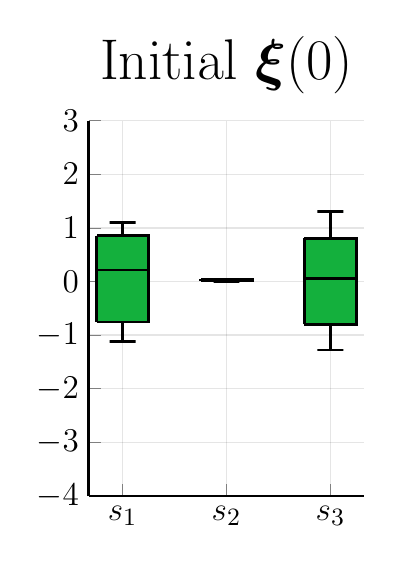
\begin{tikzpicture}[]
\begin{axis}[height = {63.5mm}, ylabel = {}, title = {Initial $\bm \xi(0)$}, xmin = {0.175}, xmax = {2.825}, ymax = {3}, xlabel = {}, unbounded coords=jump,scaled x ticks = false,xlabel style = {font = {\fontsize{18 pt}{23.400000000000002 pt}\selectfont}, color = {rgb,1:red,0.00000000;green,0.00000000;blue,0.00000000}, draw opacity = 1.0, rotate = 0.0},xmajorgrids = true,xtick = {0.5,1.5,2.5},xticklabels = {$s_1$,$s_2$,$s_3$},xtick align = inside,xticklabel style = {font = {\fontsize{13 pt}{16.900000000000002 pt}\selectfont}, color = {rgb,1:red,0.00000000;green,0.00000000;blue,0.00000000}, draw opacity = 1.0, rotate = 0.0},x grid style = {color = {rgb,1:red,0.00000000;green,0.00000000;blue,0.00000000},
draw opacity = 0.1,
line width = 0.5,
solid},axis x line* = left,x axis line style = {color = {rgb,1:red,0.00000000;green,0.00000000;blue,0.00000000},
draw opacity = 1.0,
line width = 1,
solid},scaled y ticks = false,ylabel style = {font = {\fontsize{18 pt}{23.400000000000002 pt}\selectfont}, color = {rgb,1:red,0.00000000;green,0.00000000;blue,0.00000000}, draw opacity = 1.0, rotate = 0.0},ymajorgrids = true,ytick = {-4.0,-3.0,-2.0,-1.0,0.0,1.0,2.0,3.0},yticklabels = {$-4$,$-3$,$-2$,$-1$,$0$,$1$,$2$,$3$},ytick align = inside,yticklabel style = {font = {\fontsize{13 pt}{16.900000000000002 pt}\selectfont}, color = {rgb,1:red,0.00000000;green,0.00000000;blue,0.00000000}, draw opacity = 1.0, rotate = 0.0},y grid style = {color = {rgb,1:red,0.00000000;green,0.00000000;blue,0.00000000},
draw opacity = 0.1,
line width = 0.5,
solid},axis y line* = left,y axis line style = {color = {rgb,1:red,0.00000000;green,0.00000000;blue,0.00000000},
draw opacity = 1.0,
line width = 1,
solid},    xshift = 0.0mm,
    yshift = 0.0mm,
    axis background/.style={fill={rgb,1:red,1.00000000;green,1.00000000;blue,1.00000000}}
,title style = {font = {\fontsize{22 pt}{28.6 pt}\selectfont}, color = {rgb,1:red,0.00000000;green,0.00000000;blue,0.00000000}, draw opacity = 1.0, rotate = 0.0},legend style = {color = {rgb,1:red,0.00000000;green,0.00000000;blue,0.00000000},
draw opacity = 1.0,
line width = 1,
solid,fill = {rgb,1:red,1.00000000;green,1.00000000;blue,1.00000000},font = {\fontsize{13 pt}{16.900000000000002 pt}\selectfont}},colorbar style={title=}, ymin = {-4}, width = {50.8mm}]\addplot+ [color = {rgb,1:red,0.00000000;green,0.00000000;blue,0.00000000},
draw opacity = 1.0,
line width = 1,
solid,mark = none,
mark size = 2.0,
mark options = {
    color = {rgb,1:red,0.00000000;green,0.00000000;blue,0.00000000}, draw opacity = 1.0,
    fill = {rgb,1:red,0.07843137;green,0.69019608;blue,0.23921569}, fill opacity = 1.0,
    line width = 1,
    rotate = 0,
    solid
},fill = {rgb,1:red,0.07843137;green,0.69019608;blue,0.23921569}, fill opacity=1.0,forget plot]coordinates {
(0.5, -1.1239759922027588)
(0.375, -1.1239759922027588)
(0.625, -1.1239759922027588)
(0.5, -1.1239759922027588)
(0.5, -0.7573540061712265)
};
\addplot+ [color = {rgb,1:red,0.00000000;green,0.00000000;blue,0.00000000},
draw opacity = 1.0,
line width = 1,
solid,mark = none,
mark size = 2.0,
mark options = {
    color = {rgb,1:red,0.00000000;green,0.00000000;blue,0.00000000}, draw opacity = 1.0,
    fill = {rgb,1:red,0.07843137;green,0.69019608;blue,0.23921569}, fill opacity = 1.0,
    line width = 1,
    rotate = 0,
    solid
},fill = {rgb,1:red,0.07843137;green,0.69019608;blue,0.23921569}, fill opacity=1.0,forget plot]coordinates {
(0.25, -0.7573540061712265)
(0.25, 0.21529492735862732)
(0.75, 0.21529492735862732)
(0.75, -0.7573540061712265)
(0.25, -0.7573540061712265)
};
\addplot+ [color = {rgb,1:red,0.00000000;green,0.00000000;blue,0.00000000},
draw opacity = 1.0,
line width = 1,
solid,mark = none,
mark size = 2.0,
mark options = {
    color = {rgb,1:red,0.00000000;green,0.00000000;blue,0.00000000}, draw opacity = 1.0,
    fill = {rgb,1:red,0.07843137;green,0.69019608;blue,0.23921569}, fill opacity = 1.0,
    line width = 1,
    rotate = 0,
    solid
},fill = {rgb,1:red,0.07843137;green,0.69019608;blue,0.23921569}, fill opacity=1.0,forget plot]coordinates {
(0.25, 0.8526894301176071)
(0.25, 0.21529492735862732)
(0.75, 0.21529492735862732)
(0.75, 0.8526894301176071)
(0.25, 0.8526894301176071)
};
\addplot+ [color = {rgb,1:red,0.00000000;green,0.00000000;blue,0.00000000},
draw opacity = 1.0,
line width = 1,
solid,mark = none,
mark size = 2.0,
mark options = {
    color = {rgb,1:red,0.00000000;green,0.00000000;blue,0.00000000}, draw opacity = 1.0,
    fill = {rgb,1:red,0.07843137;green,0.69019608;blue,0.23921569}, fill opacity = 1.0,
    line width = 1,
    rotate = 0,
    solid
},fill = {rgb,1:red,0.07843137;green,0.69019608;blue,0.23921569}, fill opacity=1.0,forget plot]coordinates {
(0.5, 1.0979955196380615)
(0.375, 1.0979955196380615)
(0.625, 1.0979955196380615)
(0.5, 1.0979955196380615)
(0.5, 0.8526894301176071)
};
\addplot+ [color = {rgb,1:red,0.00000000;green,0.00000000;blue,0.00000000},
draw opacity = 1.0,
line width = 1,
solid,mark = none,
mark size = 2.0,
mark options = {
    color = {rgb,1:red,0.00000000;green,0.00000000;blue,0.00000000}, draw opacity = 1.0,
    fill = {rgb,1:red,0.07843137;green,0.69019608;blue,0.23921569}, fill opacity = 1.0,
    line width = 1,
    rotate = 0,
    solid
},fill = {rgb,1:red,0.07843137;green,0.69019608;blue,0.23921569}, fill opacity=1.0,forget plot]coordinates {
(1.5, 0.005244790576398373)
(1.375, 0.005244790576398373)
(1.625, 0.005244790576398373)
(1.5, 0.005244790576398373)
(1.5, 0.01989517593756318)
};
\addplot+ [color = {rgb,1:red,0.00000000;green,0.00000000;blue,0.00000000},
draw opacity = 1.0,
line width = 1,
solid,mark = none,
mark size = 2.0,
mark options = {
    color = {rgb,1:red,0.00000000;green,0.00000000;blue,0.00000000}, draw opacity = 1.0,
    fill = {rgb,1:red,0.07843137;green,0.69019608;blue,0.23921569}, fill opacity = 1.0,
    line width = 1,
    rotate = 0,
    solid
},fill = {rgb,1:red,0.07843137;green,0.69019608;blue,0.23921569}, fill opacity=1.0,forget plot]coordinates {
(1.25, 0.01989517593756318)
(1.25, 0.02920403052121401)
(1.75, 0.02920403052121401)
(1.75, 0.01989517593756318)
(1.25, 0.01989517593756318)
};
\addplot+ [color = {rgb,1:red,0.00000000;green,0.00000000;blue,0.00000000},
draw opacity = 1.0,
line width = 1,
solid,mark = none,
mark size = 2.0,
mark options = {
    color = {rgb,1:red,0.00000000;green,0.00000000;blue,0.00000000}, draw opacity = 1.0,
    fill = {rgb,1:red,0.07843137;green,0.69019608;blue,0.23921569}, fill opacity = 1.0,
    line width = 1,
    rotate = 0,
    solid
},fill = {rgb,1:red,0.07843137;green,0.69019608;blue,0.23921569}, fill opacity=1.0,forget plot]coordinates {
(1.25, 0.03536794986575842)
(1.25, 0.02920403052121401)
(1.75, 0.02920403052121401)
(1.75, 0.03536794986575842)
(1.25, 0.03536794986575842)
};
\addplot+ [color = {rgb,1:red,0.00000000;green,0.00000000;blue,0.00000000},
draw opacity = 1.0,
line width = 1,
solid,mark = none,
mark size = 2.0,
mark options = {
    color = {rgb,1:red,0.00000000;green,0.00000000;blue,0.00000000}, draw opacity = 1.0,
    fill = {rgb,1:red,0.07843137;green,0.69019608;blue,0.23921569}, fill opacity = 1.0,
    line width = 1,
    rotate = 0,
    solid
},fill = {rgb,1:red,0.07843137;green,0.69019608;blue,0.23921569}, fill opacity=1.0,forget plot]coordinates {
(1.5, 0.04812627658247948)
(1.375, 0.04812627658247948)
(1.625, 0.04812627658247948)
(1.5, 0.04812627658247948)
(1.5, 0.03536794986575842)
};
\addplot+ [color = {rgb,1:red,0.00000000;green,0.00000000;blue,0.00000000},
draw opacity = 1.0,
line width = 1,
solid,mark = none,
mark size = 2.0,
mark options = {
    color = {rgb,1:red,0.00000000;green,0.00000000;blue,0.00000000}, draw opacity = 1.0,
    fill = {rgb,1:red,0.07843137;green,0.69019608;blue,0.23921569}, fill opacity = 1.0,
    line width = 1,
    rotate = 0,
    solid
},fill = {rgb,1:red,0.07843137;green,0.69019608;blue,0.23921569}, fill opacity=1.0,forget plot]coordinates {
(2.5, -1.2755112648010254)
(2.375, -1.2755112648010254)
(2.625, -1.2755112648010254)
(2.5, -1.2755112648010254)
(2.5, -0.799699679017067)
};
\addplot+ [color = {rgb,1:red,0.00000000;green,0.00000000;blue,0.00000000},
draw opacity = 1.0,
line width = 1,
solid,mark = none,
mark size = 2.0,
mark options = {
    color = {rgb,1:red,0.00000000;green,0.00000000;blue,0.00000000}, draw opacity = 1.0,
    fill = {rgb,1:red,0.07843137;green,0.69019608;blue,0.23921569}, fill opacity = 1.0,
    line width = 1,
    rotate = 0,
    solid
},fill = {rgb,1:red,0.07843137;green,0.69019608;blue,0.23921569}, fill opacity=1.0,forget plot]coordinates {
(2.25, -0.799699679017067)
(2.25, 0.05818364955484867)
(2.75, 0.05818364955484867)
(2.75, -0.799699679017067)
(2.25, -0.799699679017067)
};
\addplot+ [color = {rgb,1:red,0.00000000;green,0.00000000;blue,0.00000000},
draw opacity = 1.0,
line width = 1,
solid,mark = none,
mark size = 2.0,
mark options = {
    color = {rgb,1:red,0.00000000;green,0.00000000;blue,0.00000000}, draw opacity = 1.0,
    fill = {rgb,1:red,0.07843137;green,0.69019608;blue,0.23921569}, fill opacity = 1.0,
    line width = 1,
    rotate = 0,
    solid
},fill = {rgb,1:red,0.07843137;green,0.69019608;blue,0.23921569}, fill opacity=1.0,forget plot]coordinates {
(2.25, 0.802848145365715)
(2.25, 0.05818364955484867)
(2.75, 0.05818364955484867)
(2.75, 0.802848145365715)
(2.25, 0.802848145365715)
};
\addplot+ [color = {rgb,1:red,0.00000000;green,0.00000000;blue,0.00000000},
draw opacity = 1.0,
line width = 1,
solid,mark = none,
mark size = 2.0,
mark options = {
    color = {rgb,1:red,0.00000000;green,0.00000000;blue,0.00000000}, draw opacity = 1.0,
    fill = {rgb,1:red,0.07843137;green,0.69019608;blue,0.23921569}, fill opacity = 1.0,
    line width = 1,
    rotate = 0,
    solid
},fill = {rgb,1:red,0.07843137;green,0.69019608;blue,0.23921569}, fill opacity=1.0,forget plot]coordinates {
(2.5, 1.304929494857788)
(2.375, 1.304929494857788)
(2.625, 1.304929494857788)
(2.5, 1.304929494857788)
(2.5, 0.802848145365715)
};
\end{axis}

\end{tikzpicture}
}
  \resizebox{!}{.28\linewidth}{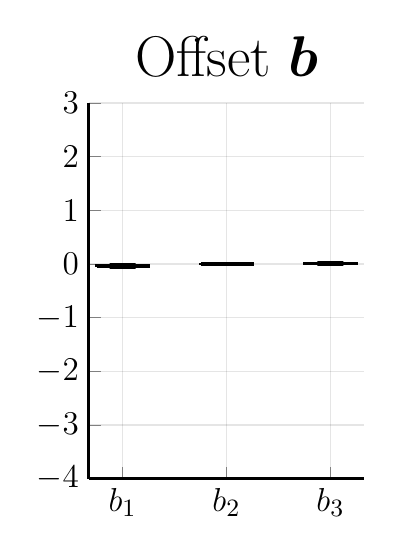
\begin{tikzpicture}[]
\begin{axis}[height = {63.5mm}, ylabel = {}, title = {Offset $\bm b$}, xmin = {0.175}, xmax = {2.825}, ymax = {3}, xlabel = {}, unbounded coords=jump,scaled x ticks = false,xlabel style = {font = {\fontsize{18 pt}{23.400000000000002 pt}\selectfont}, color = {rgb,1:red,0.00000000;green,0.00000000;blue,0.00000000}, draw opacity = 1.0, rotate = 0.0},xmajorgrids = true,xtick = {0.5,1.5,2.5},xticklabels = {$b_1$,$b_2$,$b_3$},xtick align = inside,xticklabel style = {font = {\fontsize{13 pt}{16.900000000000002 pt}\selectfont}, color = {rgb,1:red,0.00000000;green,0.00000000;blue,0.00000000}, draw opacity = 1.0, rotate = 0.0},x grid style = {color = {rgb,1:red,0.00000000;green,0.00000000;blue,0.00000000},
draw opacity = 0.1,
line width = 0.5,
solid},axis x line* = left,x axis line style = {color = {rgb,1:red,0.00000000;green,0.00000000;blue,0.00000000},
draw opacity = 1.0,
line width = 1,
solid},scaled y ticks = false,ylabel style = {font = {\fontsize{18 pt}{23.400000000000002 pt}\selectfont}, color = {rgb,1:red,0.00000000;green,0.00000000;blue,0.00000000}, draw opacity = 1.0, rotate = 0.0},ymajorgrids = true,ytick = {-4.0,-3.0,-2.0,-1.0,0.0,1.0,2.0,3.0},yticklabels = {$-4$,$-3$,$-2$,$-1$,$0$,$1$,$2$,$3$},ytick align = inside,yticklabel style = {font = {\fontsize{13 pt}{16.900000000000002 pt}\selectfont}, color = {rgb,1:red,0.00000000;green,0.00000000;blue,0.00000000}, draw opacity = 1.0, rotate = 0.0},y grid style = {color = {rgb,1:red,0.00000000;green,0.00000000;blue,0.00000000},
draw opacity = 0.1,
line width = 0.5,
solid},axis y line* = left,y axis line style = {color = {rgb,1:red,0.00000000;green,0.00000000;blue,0.00000000},
draw opacity = 1.0,
line width = 1,
solid},    xshift = 0.0mm,
    yshift = 0.0mm,
    axis background/.style={fill={rgb,1:red,1.00000000;green,1.00000000;blue,1.00000000}}
,title style = {font = {\fontsize{22 pt}{28.6 pt}\selectfont}, color = {rgb,1:red,0.00000000;green,0.00000000;blue,0.00000000}, draw opacity = 1.0, rotate = 0.0},legend style = {color = {rgb,1:red,0.00000000;green,0.00000000;blue,0.00000000},
draw opacity = 1.0,
line width = 1,
solid,fill = {rgb,1:red,1.00000000;green,1.00000000;blue,1.00000000},font = {\fontsize{13 pt}{16.900000000000002 pt}\selectfont}},colorbar style={title=}, ymin = {-4}, width = {50.8mm}]\addplot+ [color = {rgb,1:red,0.00000000;green,0.00000000;blue,0.00000000},
draw opacity = 1.0,
line width = 1,
solid,mark = none,
mark size = 2.0,
mark options = {
    color = {rgb,1:red,0.00000000;green,0.00000000;blue,0.00000000}, draw opacity = 1.0,
    fill = {rgb,1:red,0.07843137;green,0.69019608;blue,0.23921569}, fill opacity = 1.0,
    line width = 1,
    rotate = 0,
    solid
},fill = {rgb,1:red,0.07843137;green,0.69019608;blue,0.23921569}, fill opacity=1.0,forget plot]coordinates {
(0.5, -0.062348078936338425)
(0.375, -0.062348078936338425)
(0.625, -0.062348078936338425)
(0.5, -0.062348078936338425)
(0.5, -0.04346746485680342)
};
\addplot+ [color = {rgb,1:red,0.00000000;green,0.00000000;blue,0.00000000},
draw opacity = 1.0,
line width = 1,
solid,mark = none,
mark size = 2.0,
mark options = {
    color = {rgb,1:red,0.00000000;green,0.00000000;blue,0.00000000}, draw opacity = 1.0,
    fill = {rgb,1:red,0.07843137;green,0.69019608;blue,0.23921569}, fill opacity = 1.0,
    line width = 1,
    rotate = 0,
    solid
},fill = {rgb,1:red,0.07843137;green,0.69019608;blue,0.23921569}, fill opacity=1.0,forget plot]coordinates {
(0.25, -0.04346746485680342)
(0.25, -0.028916319832205772)
(0.75, -0.028916319832205772)
(0.75, -0.04346746485680342)
(0.25, -0.04346746485680342)
};
\addplot+ [color = {rgb,1:red,0.00000000;green,0.00000000;blue,0.00000000},
draw opacity = 1.0,
line width = 1,
solid,mark = none,
mark size = 2.0,
mark options = {
    color = {rgb,1:red,0.00000000;green,0.00000000;blue,0.00000000}, draw opacity = 1.0,
    fill = {rgb,1:red,0.07843137;green,0.69019608;blue,0.23921569}, fill opacity = 1.0,
    line width = 1,
    rotate = 0,
    solid
},fill = {rgb,1:red,0.07843137;green,0.69019608;blue,0.23921569}, fill opacity=1.0,forget plot]coordinates {
(0.25, -0.020901923067867756)
(0.25, -0.028916319832205772)
(0.75, -0.028916319832205772)
(0.75, -0.020901923067867756)
(0.25, -0.020901923067867756)
};
\addplot+ [color = {rgb,1:red,0.00000000;green,0.00000000;blue,0.00000000},
draw opacity = 1.0,
line width = 1,
solid,mark = none,
mark size = 2.0,
mark options = {
    color = {rgb,1:red,0.00000000;green,0.00000000;blue,0.00000000}, draw opacity = 1.0,
    fill = {rgb,1:red,0.07843137;green,0.69019608;blue,0.23921569}, fill opacity = 1.0,
    line width = 1,
    rotate = 0,
    solid
},fill = {rgb,1:red,0.07843137;green,0.69019608;blue,0.23921569}, fill opacity=1.0,forget plot]coordinates {
(0.5, -0.000460662879049778)
(0.375, -0.000460662879049778)
(0.625, -0.000460662879049778)
(0.5, -0.000460662879049778)
(0.5, -0.020901923067867756)
};
\addplot+ [color = {rgb,1:red,0.00000000;green,0.00000000;blue,0.00000000},
draw opacity = 1.0,
line width = 1,
solid,mark = none,
mark size = 2.0,
mark options = {
    color = {rgb,1:red,0.00000000;green,0.00000000;blue,0.00000000}, draw opacity = 1.0,
    fill = {rgb,1:red,0.07843137;green,0.69019608;blue,0.23921569}, fill opacity = 1.0,
    line width = 1,
    rotate = 0,
    solid
},fill = {rgb,1:red,0.07843137;green,0.69019608;blue,0.23921569}, fill opacity=1.0,forget plot]coordinates {
(1.5, -0.010381093248724937)
(1.375, -0.010381093248724937)
(1.625, -0.010381093248724937)
(1.5, -0.010381093248724937)
(1.5, -0.0025315636303275824)
};
\addplot+ [color = {rgb,1:red,0.00000000;green,0.00000000;blue,0.00000000},
draw opacity = 1.0,
line width = 1,
solid,mark = none,
mark size = 2.0,
mark options = {
    color = {rgb,1:red,0.00000000;green,0.00000000;blue,0.00000000}, draw opacity = 1.0,
    fill = {rgb,1:red,0.07843137;green,0.69019608;blue,0.23921569}, fill opacity = 1.0,
    line width = 1,
    rotate = 0,
    solid
},fill = {rgb,1:red,0.07843137;green,0.69019608;blue,0.23921569}, fill opacity=1.0,forget plot]coordinates {
(1.25, -0.0025315636303275824)
(1.25, 0.0015649637207388878)
(1.75, 0.0015649637207388878)
(1.75, -0.0025315636303275824)
(1.25, -0.0025315636303275824)
};
\addplot+ [color = {rgb,1:red,0.00000000;green,0.00000000;blue,0.00000000},
draw opacity = 1.0,
line width = 1,
solid,mark = none,
mark size = 2.0,
mark options = {
    color = {rgb,1:red,0.00000000;green,0.00000000;blue,0.00000000}, draw opacity = 1.0,
    fill = {rgb,1:red,0.07843137;green,0.69019608;blue,0.23921569}, fill opacity = 1.0,
    line width = 1,
    rotate = 0,
    solid
},fill = {rgb,1:red,0.07843137;green,0.69019608;blue,0.23921569}, fill opacity=1.0,forget plot]coordinates {
(1.25, 0.0068626245483756065)
(1.25, 0.0015649637207388878)
(1.75, 0.0015649637207388878)
(1.75, 0.0068626245483756065)
(1.25, 0.0068626245483756065)
};
\addplot+ [color = {rgb,1:red,0.00000000;green,0.00000000;blue,0.00000000},
draw opacity = 1.0,
line width = 1,
solid,mark = none,
mark size = 2.0,
mark options = {
    color = {rgb,1:red,0.00000000;green,0.00000000;blue,0.00000000}, draw opacity = 1.0,
    fill = {rgb,1:red,0.07843137;green,0.69019608;blue,0.23921569}, fill opacity = 1.0,
    line width = 1,
    rotate = 0,
    solid
},fill = {rgb,1:red,0.07843137;green,0.69019608;blue,0.23921569}, fill opacity=1.0,forget plot]coordinates {
(1.5, 0.013926548883318901)
(1.375, 0.013926548883318901)
(1.625, 0.013926548883318901)
(1.5, 0.013926548883318901)
(1.5, 0.0068626245483756065)
};
\addplot+ [color = {rgb,1:red,0.00000000;green,0.00000000;blue,0.00000000},
draw opacity = 1.0,
line width = 1,
solid,mark = none,
mark size = 2.0,
mark options = {
    color = {rgb,1:red,0.00000000;green,0.00000000;blue,0.00000000}, draw opacity = 1.0,
    fill = {rgb,1:red,0.07843137;green,0.69019608;blue,0.23921569}, fill opacity = 1.0,
    line width = 1,
    rotate = 0,
    solid
},fill = {rgb,1:red,0.07843137;green,0.69019608;blue,0.23921569}, fill opacity=1.0,forget plot]coordinates {
(2.5, -0.010155513882637024)
(2.375, -0.010155513882637024)
(2.625, -0.010155513882637024)
(2.5, -0.010155513882637024)
(2.5, 0.0009392667561769485)
};
\addplot+ [color = {rgb,1:red,0.00000000;green,0.00000000;blue,0.00000000},
draw opacity = 1.0,
line width = 1,
solid,mark = none,
mark size = 2.0,
mark options = {
    color = {rgb,1:red,0.00000000;green,0.00000000;blue,0.00000000}, draw opacity = 1.0,
    fill = {rgb,1:red,0.07843137;green,0.69019608;blue,0.23921569}, fill opacity = 1.0,
    line width = 1,
    rotate = 0,
    solid
},fill = {rgb,1:red,0.07843137;green,0.69019608;blue,0.23921569}, fill opacity=1.0,forget plot]coordinates {
(2.25, 0.0009392667561769485)
(2.25, 0.005983080714941025)
(2.75, 0.005983080714941025)
(2.75, 0.0009392667561769485)
(2.25, 0.0009392667561769485)
};
\addplot+ [color = {rgb,1:red,0.00000000;green,0.00000000;blue,0.00000000},
draw opacity = 1.0,
line width = 1,
solid,mark = none,
mark size = 2.0,
mark options = {
    color = {rgb,1:red,0.00000000;green,0.00000000;blue,0.00000000}, draw opacity = 1.0,
    fill = {rgb,1:red,0.07843137;green,0.69019608;blue,0.23921569}, fill opacity = 1.0,
    line width = 1,
    rotate = 0,
    solid
},fill = {rgb,1:red,0.07843137;green,0.69019608;blue,0.23921569}, fill opacity=1.0,forget plot]coordinates {
(2.25, 0.012997731566429138)
(2.25, 0.005983080714941025)
(2.75, 0.005983080714941025)
(2.75, 0.012997731566429138)
(2.25, 0.012997731566429138)
};
\addplot+ [color = {rgb,1:red,0.00000000;green,0.00000000;blue,0.00000000},
draw opacity = 1.0,
line width = 1,
solid,mark = none,
mark size = 2.0,
mark options = {
    color = {rgb,1:red,0.00000000;green,0.00000000;blue,0.00000000}, draw opacity = 1.0,
    fill = {rgb,1:red,0.07843137;green,0.69019608;blue,0.23921569}, fill opacity = 1.0,
    line width = 1,
    rotate = 0,
    solid
},fill = {rgb,1:red,0.07843137;green,0.69019608;blue,0.23921569}, fill opacity=1.0,forget plot]coordinates {
(2.5, 0.028738640248775482)
(2.375, 0.028738640248775482)
(2.625, 0.028738640248775482)
(2.5, 0.028738640248775482)
(2.5, 0.012997731566429138)
};
\end{axis}

\end{tikzpicture}
}
\end{frame}


\begin{frame}{Results}
  \centering
  \resizebox{\linewidth}{!}{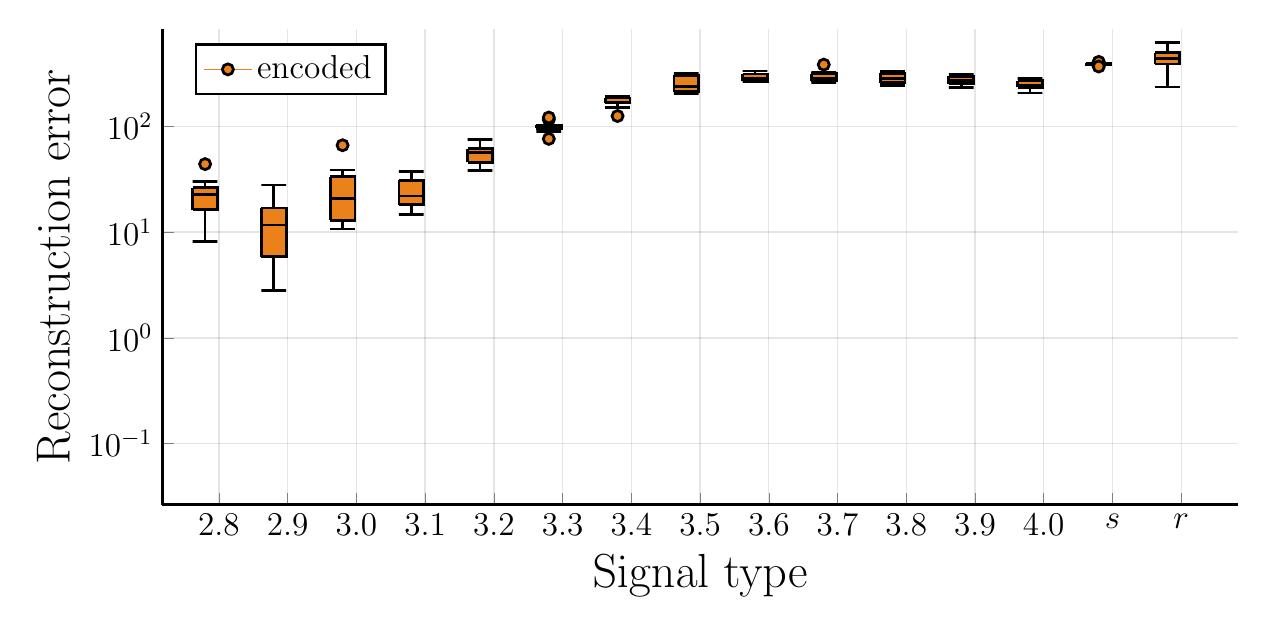
\begin{tikzpicture}[]
\begin{axis}[height = {76.2mm}, legend pos = {north west}, ylabel = {Reconstruction error}, xmin = {-0.3228}, xmax = {15.322799999999999}, ymax = {835.2283942487849}, ymode = {log}, xlabel = {Signal type}, unbounded coords=jump,scaled x ticks = false,xlabel style = {font = {\fontsize{16 pt}{20.8 pt}\selectfont}, color = {rgb,1:red,0.00000000;green,0.00000000;blue,0.00000000}, draw opacity = 1.0, rotate = 0.0},xmajorgrids = true,xtick = {0.5,1.5,2.5,3.5,4.5,5.5,6.5,7.5,8.5,9.5,10.5,11.5,12.5,13.5,14.5},xticklabels = {$2.8$,$2.9$,$3.0$,$3.1$,$3.2$,$3.3$,$3.4$,$3.5$,$3.6$,$3.7$,$3.8$,$3.9$,$4.0$,$s$,$r$},xtick align = inside,xticklabel style = {font = {\fontsize{12 pt}{15.600000000000001 pt}\selectfont}, color = {rgb,1:red,0.00000000;green,0.00000000;blue,0.00000000}, draw opacity = 1.0, rotate = 0.0},x grid style = {color = {rgb,1:red,0.00000000;green,0.00000000;blue,0.00000000},
draw opacity = 0.1,
line width = 0.5,
solid},axis x line* = left,x axis line style = {color = {rgb,1:red,0.00000000;green,0.00000000;blue,0.00000000},
draw opacity = 1.0,
line width = 1,
solid},scaled y ticks = false,ylabel style = {font = {\fontsize{16 pt}{20.8 pt}\selectfont}, color = {rgb,1:red,0.00000000;green,0.00000000;blue,0.00000000}, draw opacity = 1.0, rotate = 0.0},log basis y=10,ymajorgrids = true,ytick = {0.1,1.0,10.0,100.0},yticklabels = {$10^{-1}$,$10^{0}$,$10^{1}$,$10^{2}$},ytick align = inside,yticklabel style = {font = {\fontsize{12 pt}{15.600000000000001 pt}\selectfont}, color = {rgb,1:red,0.00000000;green,0.00000000;blue,0.00000000}, draw opacity = 1.0, rotate = 0.0},y grid style = {color = {rgb,1:red,0.00000000;green,0.00000000;blue,0.00000000},
draw opacity = 0.1,
line width = 0.5,
solid},axis y line* = left,y axis line style = {color = {rgb,1:red,0.00000000;green,0.00000000;blue,0.00000000},
draw opacity = 1.0,
line width = 1,
solid},    xshift = 0.0mm,
    yshift = 0.0mm,
    axis background/.style={fill={rgb,1:red,1.00000000;green,1.00000000;blue,1.00000000}}
,legend style = {color = {rgb,1:red,0.00000000;green,0.00000000;blue,0.00000000},
draw opacity = 1.0,
line width = 1,
solid,fill = {rgb,1:red,1.00000000;green,1.00000000;blue,1.00000000},font = {\fontsize{12 pt}{15.600000000000001 pt}\selectfont}},colorbar style={title=}, ymin = {0.026513221702982547}, width = {152.4mm}]\addplot+[draw=none, color = {rgb,1:red,0.92156863;green,0.50588235;blue,0.10588235},
draw opacity = 1.0,
line width = 0,
solid,mark = *,
mark size = 2.0,
mark options = {
    color = {rgb,1:red,0.00000000;green,0.00000000;blue,0.00000000}, draw opacity = 1.0,
    fill = {rgb,1:red,0.92156863;green,0.50588235;blue,0.10588235}, fill opacity = 1.0,
    line width = 1,
    rotate = 0,
    solid
}] coordinates {
(0.3, 44.06361770629883)
(2.3, 66.4576416015625)
(5.3, 116.00747680664062)
(5.3, 76.35958099365234)
(5.3, 121.595947265625)
(6.3, 125.59378814697266)
(9.3, 384.752197265625)
(13.3, 374.16156005859375)
(13.3, 405.60662841796875)
(13.3, 408.53326416015625)
(13.3, 369.4435729980469)
};
\addlegendentry{encoded}
\addplot+ [color = {rgb,1:red,0.00000000;green,0.00000000;blue,0.00000000},
draw opacity = 1.0,
line width = 1,
solid,mark = none,
mark size = 2.0,
mark options = {
    color = {rgb,1:red,0.00000000;green,0.00000000;blue,0.00000000}, draw opacity = 1.0,
    fill = {rgb,1:red,0.92156863;green,0.50588235;blue,0.10588235}, fill opacity = 1.0,
    line width = 1,
    rotate = 0,
    solid
},fill = {rgb,1:red,0.92156863;green,0.50588235;blue,0.10588235}, fill opacity=1.0,forget plot]coordinates {
(0.3, 8.204172134399414)
(0.11999999999999997, 8.204172134399414)
(0.48, 8.204172134399414)
(0.3, 8.204172134399414)
(0.3, 16.3089656829834)
};
\addplot+ [color = {rgb,1:red,0.00000000;green,0.00000000;blue,0.00000000},
draw opacity = 1.0,
line width = 1,
solid,mark = none,
mark size = 2.0,
mark options = {
    color = {rgb,1:red,0.00000000;green,0.00000000;blue,0.00000000}, draw opacity = 1.0,
    fill = {rgb,1:red,0.92156863;green,0.50588235;blue,0.10588235}, fill opacity = 1.0,
    line width = 1,
    rotate = 0,
    solid
},fill = {rgb,1:red,0.92156863;green,0.50588235;blue,0.10588235}, fill opacity=1.0,forget plot]coordinates {
(0.11999999999999997, 16.3089656829834)
(0.11999999999999997, 22.558713912963867)
(0.48, 22.558713912963867)
(0.48, 16.3089656829834)
(0.11999999999999997, 16.3089656829834)
};
\addplot+ [color = {rgb,1:red,0.00000000;green,0.00000000;blue,0.00000000},
draw opacity = 1.0,
line width = 1,
solid,mark = none,
mark size = 2.0,
mark options = {
    color = {rgb,1:red,0.00000000;green,0.00000000;blue,0.00000000}, draw opacity = 1.0,
    fill = {rgb,1:red,0.92156863;green,0.50588235;blue,0.10588235}, fill opacity = 1.0,
    line width = 1,
    rotate = 0,
    solid
},fill = {rgb,1:red,0.92156863;green,0.50588235;blue,0.10588235}, fill opacity=1.0,forget plot]coordinates {
(0.11999999999999997, 26.31829071044922)
(0.11999999999999997, 22.558713912963867)
(0.48, 22.558713912963867)
(0.48, 26.31829071044922)
(0.11999999999999997, 26.31829071044922)
};
\addplot+ [color = {rgb,1:red,0.00000000;green,0.00000000;blue,0.00000000},
draw opacity = 1.0,
line width = 1,
solid,mark = none,
mark size = 2.0,
mark options = {
    color = {rgb,1:red,0.00000000;green,0.00000000;blue,0.00000000}, draw opacity = 1.0,
    fill = {rgb,1:red,0.92156863;green,0.50588235;blue,0.10588235}, fill opacity = 1.0,
    line width = 1,
    rotate = 0,
    solid
},fill = {rgb,1:red,0.92156863;green,0.50588235;blue,0.10588235}, fill opacity=1.0,forget plot]coordinates {
(0.3, 29.960102081298828)
(0.11999999999999997, 29.960102081298828)
(0.48, 29.960102081298828)
(0.3, 29.960102081298828)
(0.3, 26.31829071044922)
};
\addplot+ [color = {rgb,1:red,0.00000000;green,0.00000000;blue,0.00000000},
draw opacity = 1.0,
line width = 1,
solid,mark = none,
mark size = 2.0,
mark options = {
    color = {rgb,1:red,0.00000000;green,0.00000000;blue,0.00000000}, draw opacity = 1.0,
    fill = {rgb,1:red,0.92156863;green,0.50588235;blue,0.10588235}, fill opacity = 1.0,
    line width = 1,
    rotate = 0,
    solid
},fill = {rgb,1:red,0.92156863;green,0.50588235;blue,0.10588235}, fill opacity=1.0,forget plot]coordinates {
(1.3, 2.7880234718322754)
(1.12, 2.7880234718322754)
(1.48, 2.7880234718322754)
(1.3, 2.7880234718322754)
(1.3, 5.857234001159668)
};
\addplot+ [color = {rgb,1:red,0.00000000;green,0.00000000;blue,0.00000000},
draw opacity = 1.0,
line width = 1,
solid,mark = none,
mark size = 2.0,
mark options = {
    color = {rgb,1:red,0.00000000;green,0.00000000;blue,0.00000000}, draw opacity = 1.0,
    fill = {rgb,1:red,0.92156863;green,0.50588235;blue,0.10588235}, fill opacity = 1.0,
    line width = 1,
    rotate = 0,
    solid
},fill = {rgb,1:red,0.92156863;green,0.50588235;blue,0.10588235}, fill opacity=1.0,forget plot]coordinates {
(1.12, 5.857234001159668)
(1.12, 11.678890228271484)
(1.48, 11.678890228271484)
(1.48, 5.857234001159668)
(1.12, 5.857234001159668)
};
\addplot+ [color = {rgb,1:red,0.00000000;green,0.00000000;blue,0.00000000},
draw opacity = 1.0,
line width = 1,
solid,mark = none,
mark size = 2.0,
mark options = {
    color = {rgb,1:red,0.00000000;green,0.00000000;blue,0.00000000}, draw opacity = 1.0,
    fill = {rgb,1:red,0.92156863;green,0.50588235;blue,0.10588235}, fill opacity = 1.0,
    line width = 1,
    rotate = 0,
    solid
},fill = {rgb,1:red,0.92156863;green,0.50588235;blue,0.10588235}, fill opacity=1.0,forget plot]coordinates {
(1.12, 16.91464328765869)
(1.12, 11.678890228271484)
(1.48, 11.678890228271484)
(1.48, 16.91464328765869)
(1.12, 16.91464328765869)
};
\addplot+ [color = {rgb,1:red,0.00000000;green,0.00000000;blue,0.00000000},
draw opacity = 1.0,
line width = 1,
solid,mark = none,
mark size = 2.0,
mark options = {
    color = {rgb,1:red,0.00000000;green,0.00000000;blue,0.00000000}, draw opacity = 1.0,
    fill = {rgb,1:red,0.92156863;green,0.50588235;blue,0.10588235}, fill opacity = 1.0,
    line width = 1,
    rotate = 0,
    solid
},fill = {rgb,1:red,0.92156863;green,0.50588235;blue,0.10588235}, fill opacity=1.0,forget plot]coordinates {
(1.3, 27.9256649017334)
(1.12, 27.9256649017334)
(1.48, 27.9256649017334)
(1.3, 27.9256649017334)
(1.3, 16.91464328765869)
};
\addplot+ [color = {rgb,1:red,0.00000000;green,0.00000000;blue,0.00000000},
draw opacity = 1.0,
line width = 1,
solid,mark = none,
mark size = 2.0,
mark options = {
    color = {rgb,1:red,0.00000000;green,0.00000000;blue,0.00000000}, draw opacity = 1.0,
    fill = {rgb,1:red,0.92156863;green,0.50588235;blue,0.10588235}, fill opacity = 1.0,
    line width = 1,
    rotate = 0,
    solid
},fill = {rgb,1:red,0.92156863;green,0.50588235;blue,0.10588235}, fill opacity=1.0,forget plot]coordinates {
(2.3, 10.7005615234375)
(2.1199999999999997, 10.7005615234375)
(2.48, 10.7005615234375)
(2.3, 10.7005615234375)
(2.3, 12.931447505950928)
};
\addplot+ [color = {rgb,1:red,0.00000000;green,0.00000000;blue,0.00000000},
draw opacity = 1.0,
line width = 1,
solid,mark = none,
mark size = 2.0,
mark options = {
    color = {rgb,1:red,0.00000000;green,0.00000000;blue,0.00000000}, draw opacity = 1.0,
    fill = {rgb,1:red,0.92156863;green,0.50588235;blue,0.10588235}, fill opacity = 1.0,
    line width = 1,
    rotate = 0,
    solid
},fill = {rgb,1:red,0.92156863;green,0.50588235;blue,0.10588235}, fill opacity=1.0,forget plot]coordinates {
(2.1199999999999997, 12.931447505950928)
(2.1199999999999997, 20.765978813171387)
(2.48, 20.765978813171387)
(2.48, 12.931447505950928)
(2.1199999999999997, 12.931447505950928)
};
\addplot+ [color = {rgb,1:red,0.00000000;green,0.00000000;blue,0.00000000},
draw opacity = 1.0,
line width = 1,
solid,mark = none,
mark size = 2.0,
mark options = {
    color = {rgb,1:red,0.00000000;green,0.00000000;blue,0.00000000}, draw opacity = 1.0,
    fill = {rgb,1:red,0.92156863;green,0.50588235;blue,0.10588235}, fill opacity = 1.0,
    line width = 1,
    rotate = 0,
    solid
},fill = {rgb,1:red,0.92156863;green,0.50588235;blue,0.10588235}, fill opacity=1.0,forget plot]coordinates {
(2.1199999999999997, 33.54420804977417)
(2.1199999999999997, 20.765978813171387)
(2.48, 20.765978813171387)
(2.48, 33.54420804977417)
(2.1199999999999997, 33.54420804977417)
};
\addplot+ [color = {rgb,1:red,0.00000000;green,0.00000000;blue,0.00000000},
draw opacity = 1.0,
line width = 1,
solid,mark = none,
mark size = 2.0,
mark options = {
    color = {rgb,1:red,0.00000000;green,0.00000000;blue,0.00000000}, draw opacity = 1.0,
    fill = {rgb,1:red,0.92156863;green,0.50588235;blue,0.10588235}, fill opacity = 1.0,
    line width = 1,
    rotate = 0,
    solid
},fill = {rgb,1:red,0.92156863;green,0.50588235;blue,0.10588235}, fill opacity=1.0,forget plot]coordinates {
(2.3, 38.70692443847656)
(2.1199999999999997, 38.70692443847656)
(2.48, 38.70692443847656)
(2.3, 38.70692443847656)
(2.3, 33.54420804977417)
};
\addplot+ [color = {rgb,1:red,0.00000000;green,0.00000000;blue,0.00000000},
draw opacity = 1.0,
line width = 1,
solid,mark = none,
mark size = 2.0,
mark options = {
    color = {rgb,1:red,0.00000000;green,0.00000000;blue,0.00000000}, draw opacity = 1.0,
    fill = {rgb,1:red,0.92156863;green,0.50588235;blue,0.10588235}, fill opacity = 1.0,
    line width = 1,
    rotate = 0,
    solid
},fill = {rgb,1:red,0.92156863;green,0.50588235;blue,0.10588235}, fill opacity=1.0,forget plot]coordinates {
(3.3, 14.816097259521484)
(3.1199999999999997, 14.816097259521484)
(3.48, 14.816097259521484)
(3.3, 14.816097259521484)
(3.3, 18.226701736450195)
};
\addplot+ [color = {rgb,1:red,0.00000000;green,0.00000000;blue,0.00000000},
draw opacity = 1.0,
line width = 1,
solid,mark = none,
mark size = 2.0,
mark options = {
    color = {rgb,1:red,0.00000000;green,0.00000000;blue,0.00000000}, draw opacity = 1.0,
    fill = {rgb,1:red,0.92156863;green,0.50588235;blue,0.10588235}, fill opacity = 1.0,
    line width = 1,
    rotate = 0,
    solid
},fill = {rgb,1:red,0.92156863;green,0.50588235;blue,0.10588235}, fill opacity=1.0,forget plot]coordinates {
(3.1199999999999997, 18.226701736450195)
(3.1199999999999997, 22.01521110534668)
(3.48, 22.01521110534668)
(3.48, 18.226701736450195)
(3.1199999999999997, 18.226701736450195)
};
\addplot+ [color = {rgb,1:red,0.00000000;green,0.00000000;blue,0.00000000},
draw opacity = 1.0,
line width = 1,
solid,mark = none,
mark size = 2.0,
mark options = {
    color = {rgb,1:red,0.00000000;green,0.00000000;blue,0.00000000}, draw opacity = 1.0,
    fill = {rgb,1:red,0.92156863;green,0.50588235;blue,0.10588235}, fill opacity = 1.0,
    line width = 1,
    rotate = 0,
    solid
},fill = {rgb,1:red,0.92156863;green,0.50588235;blue,0.10588235}, fill opacity=1.0,forget plot]coordinates {
(3.1199999999999997, 30.843246936798096)
(3.1199999999999997, 22.01521110534668)
(3.48, 22.01521110534668)
(3.48, 30.843246936798096)
(3.1199999999999997, 30.843246936798096)
};
\addplot+ [color = {rgb,1:red,0.00000000;green,0.00000000;blue,0.00000000},
draw opacity = 1.0,
line width = 1,
solid,mark = none,
mark size = 2.0,
mark options = {
    color = {rgb,1:red,0.00000000;green,0.00000000;blue,0.00000000}, draw opacity = 1.0,
    fill = {rgb,1:red,0.92156863;green,0.50588235;blue,0.10588235}, fill opacity = 1.0,
    line width = 1,
    rotate = 0,
    solid
},fill = {rgb,1:red,0.92156863;green,0.50588235;blue,0.10588235}, fill opacity=1.0,forget plot]coordinates {
(3.3, 37.649349212646484)
(3.1199999999999997, 37.649349212646484)
(3.48, 37.649349212646484)
(3.3, 37.649349212646484)
(3.3, 30.843246936798096)
};
\addplot+ [color = {rgb,1:red,0.00000000;green,0.00000000;blue,0.00000000},
draw opacity = 1.0,
line width = 1,
solid,mark = none,
mark size = 2.0,
mark options = {
    color = {rgb,1:red,0.00000000;green,0.00000000;blue,0.00000000}, draw opacity = 1.0,
    fill = {rgb,1:red,0.92156863;green,0.50588235;blue,0.10588235}, fill opacity = 1.0,
    line width = 1,
    rotate = 0,
    solid
},fill = {rgb,1:red,0.92156863;green,0.50588235;blue,0.10588235}, fill opacity=1.0,forget plot]coordinates {
(4.3, 38.598915100097656)
(4.12, 38.598915100097656)
(4.4799999999999995, 38.598915100097656)
(4.3, 38.598915100097656)
(4.3, 45.87193298339844)
};
\addplot+ [color = {rgb,1:red,0.00000000;green,0.00000000;blue,0.00000000},
draw opacity = 1.0,
line width = 1,
solid,mark = none,
mark size = 2.0,
mark options = {
    color = {rgb,1:red,0.00000000;green,0.00000000;blue,0.00000000}, draw opacity = 1.0,
    fill = {rgb,1:red,0.92156863;green,0.50588235;blue,0.10588235}, fill opacity = 1.0,
    line width = 1,
    rotate = 0,
    solid
},fill = {rgb,1:red,0.92156863;green,0.50588235;blue,0.10588235}, fill opacity=1.0,forget plot]coordinates {
(4.12, 45.87193298339844)
(4.12, 56.44198417663574)
(4.4799999999999995, 56.44198417663574)
(4.4799999999999995, 45.87193298339844)
(4.12, 45.87193298339844)
};
\addplot+ [color = {rgb,1:red,0.00000000;green,0.00000000;blue,0.00000000},
draw opacity = 1.0,
line width = 1,
solid,mark = none,
mark size = 2.0,
mark options = {
    color = {rgb,1:red,0.00000000;green,0.00000000;blue,0.00000000}, draw opacity = 1.0,
    fill = {rgb,1:red,0.92156863;green,0.50588235;blue,0.10588235}, fill opacity = 1.0,
    line width = 1,
    rotate = 0,
    solid
},fill = {rgb,1:red,0.92156863;green,0.50588235;blue,0.10588235}, fill opacity=1.0,forget plot]coordinates {
(4.12, 61.80284023284912)
(4.12, 56.44198417663574)
(4.4799999999999995, 56.44198417663574)
(4.4799999999999995, 61.80284023284912)
(4.12, 61.80284023284912)
};
\addplot+ [color = {rgb,1:red,0.00000000;green,0.00000000;blue,0.00000000},
draw opacity = 1.0,
line width = 1,
solid,mark = none,
mark size = 2.0,
mark options = {
    color = {rgb,1:red,0.00000000;green,0.00000000;blue,0.00000000}, draw opacity = 1.0,
    fill = {rgb,1:red,0.92156863;green,0.50588235;blue,0.10588235}, fill opacity = 1.0,
    line width = 1,
    rotate = 0,
    solid
},fill = {rgb,1:red,0.92156863;green,0.50588235;blue,0.10588235}, fill opacity=1.0,forget plot]coordinates {
(4.3, 75.34232330322266)
(4.12, 75.34232330322266)
(4.4799999999999995, 75.34232330322266)
(4.3, 75.34232330322266)
(4.3, 61.80284023284912)
};
\addplot+ [color = {rgb,1:red,0.00000000;green,0.00000000;blue,0.00000000},
draw opacity = 1.0,
line width = 1,
solid,mark = none,
mark size = 2.0,
mark options = {
    color = {rgb,1:red,0.00000000;green,0.00000000;blue,0.00000000}, draw opacity = 1.0,
    fill = {rgb,1:red,0.92156863;green,0.50588235;blue,0.10588235}, fill opacity = 1.0,
    line width = 1,
    rotate = 0,
    solid
},fill = {rgb,1:red,0.92156863;green,0.50588235;blue,0.10588235}, fill opacity=1.0,forget plot]coordinates {
(5.3, 89.34620666503906)
(5.12, 89.34620666503906)
(5.4799999999999995, 89.34620666503906)
(5.3, 89.34620666503906)
(5.3, 95.83408737182617)
};
\addplot+ [color = {rgb,1:red,0.00000000;green,0.00000000;blue,0.00000000},
draw opacity = 1.0,
line width = 1,
solid,mark = none,
mark size = 2.0,
mark options = {
    color = {rgb,1:red,0.00000000;green,0.00000000;blue,0.00000000}, draw opacity = 1.0,
    fill = {rgb,1:red,0.92156863;green,0.50588235;blue,0.10588235}, fill opacity = 1.0,
    line width = 1,
    rotate = 0,
    solid
},fill = {rgb,1:red,0.92156863;green,0.50588235;blue,0.10588235}, fill opacity=1.0,forget plot]coordinates {
(5.12, 95.83408737182617)
(5.12, 98.83730697631836)
(5.4799999999999995, 98.83730697631836)
(5.4799999999999995, 95.83408737182617)
(5.12, 95.83408737182617)
};
\addplot+ [color = {rgb,1:red,0.00000000;green,0.00000000;blue,0.00000000},
draw opacity = 1.0,
line width = 1,
solid,mark = none,
mark size = 2.0,
mark options = {
    color = {rgb,1:red,0.00000000;green,0.00000000;blue,0.00000000}, draw opacity = 1.0,
    fill = {rgb,1:red,0.92156863;green,0.50588235;blue,0.10588235}, fill opacity = 1.0,
    line width = 1,
    rotate = 0,
    solid
},fill = {rgb,1:red,0.92156863;green,0.50588235;blue,0.10588235}, fill opacity=1.0,forget plot]coordinates {
(5.12, 102.3152027130127)
(5.12, 98.83730697631836)
(5.4799999999999995, 98.83730697631836)
(5.4799999999999995, 102.3152027130127)
(5.12, 102.3152027130127)
};
\addplot+ [color = {rgb,1:red,0.00000000;green,0.00000000;blue,0.00000000},
draw opacity = 1.0,
line width = 1,
solid,mark = none,
mark size = 2.0,
mark options = {
    color = {rgb,1:red,0.00000000;green,0.00000000;blue,0.00000000}, draw opacity = 1.0,
    fill = {rgb,1:red,0.92156863;green,0.50588235;blue,0.10588235}, fill opacity = 1.0,
    line width = 1,
    rotate = 0,
    solid
},fill = {rgb,1:red,0.92156863;green,0.50588235;blue,0.10588235}, fill opacity=1.0,forget plot]coordinates {
(5.3, 102.64289855957031)
(5.12, 102.64289855957031)
(5.4799999999999995, 102.64289855957031)
(5.3, 102.64289855957031)
(5.3, 102.3152027130127)
};
\addplot+ [color = {rgb,1:red,0.00000000;green,0.00000000;blue,0.00000000},
draw opacity = 1.0,
line width = 1,
solid,mark = none,
mark size = 2.0,
mark options = {
    color = {rgb,1:red,0.00000000;green,0.00000000;blue,0.00000000}, draw opacity = 1.0,
    fill = {rgb,1:red,0.92156863;green,0.50588235;blue,0.10588235}, fill opacity = 1.0,
    line width = 1,
    rotate = 0,
    solid
},fill = {rgb,1:red,0.92156863;green,0.50588235;blue,0.10588235}, fill opacity=1.0,forget plot]coordinates {
(6.3, 151.41188049316406)
(6.12, 151.41188049316406)
(6.4799999999999995, 151.41188049316406)
(6.3, 151.41188049316406)
(6.3, 167.3861846923828)
};
\addplot+ [color = {rgb,1:red,0.00000000;green,0.00000000;blue,0.00000000},
draw opacity = 1.0,
line width = 1,
solid,mark = none,
mark size = 2.0,
mark options = {
    color = {rgb,1:red,0.00000000;green,0.00000000;blue,0.00000000}, draw opacity = 1.0,
    fill = {rgb,1:red,0.92156863;green,0.50588235;blue,0.10588235}, fill opacity = 1.0,
    line width = 1,
    rotate = 0,
    solid
},fill = {rgb,1:red,0.92156863;green,0.50588235;blue,0.10588235}, fill opacity=1.0,forget plot]coordinates {
(6.12, 167.3861846923828)
(6.12, 170.06918334960938)
(6.4799999999999995, 170.06918334960938)
(6.4799999999999995, 167.3861846923828)
(6.12, 167.3861846923828)
};
\addplot+ [color = {rgb,1:red,0.00000000;green,0.00000000;blue,0.00000000},
draw opacity = 1.0,
line width = 1,
solid,mark = none,
mark size = 2.0,
mark options = {
    color = {rgb,1:red,0.00000000;green,0.00000000;blue,0.00000000}, draw opacity = 1.0,
    fill = {rgb,1:red,0.92156863;green,0.50588235;blue,0.10588235}, fill opacity = 1.0,
    line width = 1,
    rotate = 0,
    solid
},fill = {rgb,1:red,0.92156863;green,0.50588235;blue,0.10588235}, fill opacity=1.0,forget plot]coordinates {
(6.12, 186.0583267211914)
(6.12, 170.06918334960938)
(6.4799999999999995, 170.06918334960938)
(6.4799999999999995, 186.0583267211914)
(6.12, 186.0583267211914)
};
\addplot+ [color = {rgb,1:red,0.00000000;green,0.00000000;blue,0.00000000},
draw opacity = 1.0,
line width = 1,
solid,mark = none,
mark size = 2.0,
mark options = {
    color = {rgb,1:red,0.00000000;green,0.00000000;blue,0.00000000}, draw opacity = 1.0,
    fill = {rgb,1:red,0.92156863;green,0.50588235;blue,0.10588235}, fill opacity = 1.0,
    line width = 1,
    rotate = 0,
    solid
},fill = {rgb,1:red,0.92156863;green,0.50588235;blue,0.10588235}, fill opacity=1.0,forget plot]coordinates {
(6.3, 192.79783630371094)
(6.12, 192.79783630371094)
(6.4799999999999995, 192.79783630371094)
(6.3, 192.79783630371094)
(6.3, 186.0583267211914)
};
\addplot+ [color = {rgb,1:red,0.00000000;green,0.00000000;blue,0.00000000},
draw opacity = 1.0,
line width = 1,
solid,mark = none,
mark size = 2.0,
mark options = {
    color = {rgb,1:red,0.00000000;green,0.00000000;blue,0.00000000}, draw opacity = 1.0,
    fill = {rgb,1:red,0.92156863;green,0.50588235;blue,0.10588235}, fill opacity = 1.0,
    line width = 1,
    rotate = 0,
    solid
},fill = {rgb,1:red,0.92156863;green,0.50588235;blue,0.10588235}, fill opacity=1.0,forget plot]coordinates {
(7.3, 205.65560913085938)
(7.12, 205.65560913085938)
(7.4799999999999995, 205.65560913085938)
(7.3, 205.65560913085938)
(7.3, 213.2966423034668)
};
\addplot+ [color = {rgb,1:red,0.00000000;green,0.00000000;blue,0.00000000},
draw opacity = 1.0,
line width = 1,
solid,mark = none,
mark size = 2.0,
mark options = {
    color = {rgb,1:red,0.00000000;green,0.00000000;blue,0.00000000}, draw opacity = 1.0,
    fill = {rgb,1:red,0.92156863;green,0.50588235;blue,0.10588235}, fill opacity = 1.0,
    line width = 1,
    rotate = 0,
    solid
},fill = {rgb,1:red,0.92156863;green,0.50588235;blue,0.10588235}, fill opacity=1.0,forget plot]coordinates {
(7.12, 213.2966423034668)
(7.12, 238.21907806396484)
(7.4799999999999995, 238.21907806396484)
(7.4799999999999995, 213.2966423034668)
(7.12, 213.2966423034668)
};
\addplot+ [color = {rgb,1:red,0.00000000;green,0.00000000;blue,0.00000000},
draw opacity = 1.0,
line width = 1,
solid,mark = none,
mark size = 2.0,
mark options = {
    color = {rgb,1:red,0.00000000;green,0.00000000;blue,0.00000000}, draw opacity = 1.0,
    fill = {rgb,1:red,0.92156863;green,0.50588235;blue,0.10588235}, fill opacity = 1.0,
    line width = 1,
    rotate = 0,
    solid
},fill = {rgb,1:red,0.92156863;green,0.50588235;blue,0.10588235}, fill opacity=1.0,forget plot]coordinates {
(7.12, 303.9123764038086)
(7.12, 238.21907806396484)
(7.4799999999999995, 238.21907806396484)
(7.4799999999999995, 303.9123764038086)
(7.12, 303.9123764038086)
};
\addplot+ [color = {rgb,1:red,0.00000000;green,0.00000000;blue,0.00000000},
draw opacity = 1.0,
line width = 1,
solid,mark = none,
mark size = 2.0,
mark options = {
    color = {rgb,1:red,0.00000000;green,0.00000000;blue,0.00000000}, draw opacity = 1.0,
    fill = {rgb,1:red,0.92156863;green,0.50588235;blue,0.10588235}, fill opacity = 1.0,
    line width = 1,
    rotate = 0,
    solid
},fill = {rgb,1:red,0.92156863;green,0.50588235;blue,0.10588235}, fill opacity=1.0,forget plot]coordinates {
(7.3, 315.68939208984375)
(7.12, 315.68939208984375)
(7.4799999999999995, 315.68939208984375)
(7.3, 315.68939208984375)
(7.3, 303.9123764038086)
};
\addplot+ [color = {rgb,1:red,0.00000000;green,0.00000000;blue,0.00000000},
draw opacity = 1.0,
line width = 1,
solid,mark = none,
mark size = 2.0,
mark options = {
    color = {rgb,1:red,0.00000000;green,0.00000000;blue,0.00000000}, draw opacity = 1.0,
    fill = {rgb,1:red,0.92156863;green,0.50588235;blue,0.10588235}, fill opacity = 1.0,
    line width = 1,
    rotate = 0,
    solid
},fill = {rgb,1:red,0.92156863;green,0.50588235;blue,0.10588235}, fill opacity=1.0,forget plot]coordinates {
(8.3, 264.95477294921875)
(8.120000000000001, 264.95477294921875)
(8.48, 264.95477294921875)
(8.3, 264.95477294921875)
(8.3, 266.86964416503906)
};
\addplot+ [color = {rgb,1:red,0.00000000;green,0.00000000;blue,0.00000000},
draw opacity = 1.0,
line width = 1,
solid,mark = none,
mark size = 2.0,
mark options = {
    color = {rgb,1:red,0.00000000;green,0.00000000;blue,0.00000000}, draw opacity = 1.0,
    fill = {rgb,1:red,0.92156863;green,0.50588235;blue,0.10588235}, fill opacity = 1.0,
    line width = 1,
    rotate = 0,
    solid
},fill = {rgb,1:red,0.92156863;green,0.50588235;blue,0.10588235}, fill opacity=1.0,forget plot]coordinates {
(8.120000000000001, 266.86964416503906)
(8.120000000000001, 283.7917938232422)
(8.48, 283.7917938232422)
(8.48, 266.86964416503906)
(8.120000000000001, 266.86964416503906)
};
\addplot+ [color = {rgb,1:red,0.00000000;green,0.00000000;blue,0.00000000},
draw opacity = 1.0,
line width = 1,
solid,mark = none,
mark size = 2.0,
mark options = {
    color = {rgb,1:red,0.00000000;green,0.00000000;blue,0.00000000}, draw opacity = 1.0,
    fill = {rgb,1:red,0.92156863;green,0.50588235;blue,0.10588235}, fill opacity = 1.0,
    line width = 1,
    rotate = 0,
    solid
},fill = {rgb,1:red,0.92156863;green,0.50588235;blue,0.10588235}, fill opacity=1.0,forget plot]coordinates {
(8.120000000000001, 314.2527084350586)
(8.120000000000001, 283.7917938232422)
(8.48, 283.7917938232422)
(8.48, 314.2527084350586)
(8.120000000000001, 314.2527084350586)
};
\addplot+ [color = {rgb,1:red,0.00000000;green,0.00000000;blue,0.00000000},
draw opacity = 1.0,
line width = 1,
solid,mark = none,
mark size = 2.0,
mark options = {
    color = {rgb,1:red,0.00000000;green,0.00000000;blue,0.00000000}, draw opacity = 1.0,
    fill = {rgb,1:red,0.92156863;green,0.50588235;blue,0.10588235}, fill opacity = 1.0,
    line width = 1,
    rotate = 0,
    solid
},fill = {rgb,1:red,0.92156863;green,0.50588235;blue,0.10588235}, fill opacity=1.0,forget plot]coordinates {
(8.3, 334.311767578125)
(8.120000000000001, 334.311767578125)
(8.48, 334.311767578125)
(8.3, 334.311767578125)
(8.3, 314.2527084350586)
};
\addplot+ [color = {rgb,1:red,0.00000000;green,0.00000000;blue,0.00000000},
draw opacity = 1.0,
line width = 1,
solid,mark = none,
mark size = 2.0,
mark options = {
    color = {rgb,1:red,0.00000000;green,0.00000000;blue,0.00000000}, draw opacity = 1.0,
    fill = {rgb,1:red,0.92156863;green,0.50588235;blue,0.10588235}, fill opacity = 1.0,
    line width = 1,
    rotate = 0,
    solid
},fill = {rgb,1:red,0.92156863;green,0.50588235;blue,0.10588235}, fill opacity=1.0,forget plot]coordinates {
(9.3, 262.7439880371094)
(9.120000000000001, 262.7439880371094)
(9.48, 262.7439880371094)
(9.3, 262.7439880371094)
(9.3, 272.1040573120117)
};
\addplot+ [color = {rgb,1:red,0.00000000;green,0.00000000;blue,0.00000000},
draw opacity = 1.0,
line width = 1,
solid,mark = none,
mark size = 2.0,
mark options = {
    color = {rgb,1:red,0.00000000;green,0.00000000;blue,0.00000000}, draw opacity = 1.0,
    fill = {rgb,1:red,0.92156863;green,0.50588235;blue,0.10588235}, fill opacity = 1.0,
    line width = 1,
    rotate = 0,
    solid
},fill = {rgb,1:red,0.92156863;green,0.50588235;blue,0.10588235}, fill opacity=1.0,forget plot]coordinates {
(9.120000000000001, 272.1040573120117)
(9.120000000000001, 284.98338317871094)
(9.48, 284.98338317871094)
(9.48, 272.1040573120117)
(9.120000000000001, 272.1040573120117)
};
\addplot+ [color = {rgb,1:red,0.00000000;green,0.00000000;blue,0.00000000},
draw opacity = 1.0,
line width = 1,
solid,mark = none,
mark size = 2.0,
mark options = {
    color = {rgb,1:red,0.00000000;green,0.00000000;blue,0.00000000}, draw opacity = 1.0,
    fill = {rgb,1:red,0.92156863;green,0.50588235;blue,0.10588235}, fill opacity = 1.0,
    line width = 1,
    rotate = 0,
    solid
},fill = {rgb,1:red,0.92156863;green,0.50588235;blue,0.10588235}, fill opacity=1.0,forget plot]coordinates {
(9.120000000000001, 315.8684844970703)
(9.120000000000001, 284.98338317871094)
(9.48, 284.98338317871094)
(9.48, 315.8684844970703)
(9.120000000000001, 315.8684844970703)
};
\addplot+ [color = {rgb,1:red,0.00000000;green,0.00000000;blue,0.00000000},
draw opacity = 1.0,
line width = 1,
solid,mark = none,
mark size = 2.0,
mark options = {
    color = {rgb,1:red,0.00000000;green,0.00000000;blue,0.00000000}, draw opacity = 1.0,
    fill = {rgb,1:red,0.92156863;green,0.50588235;blue,0.10588235}, fill opacity = 1.0,
    line width = 1,
    rotate = 0,
    solid
},fill = {rgb,1:red,0.92156863;green,0.50588235;blue,0.10588235}, fill opacity=1.0,forget plot]coordinates {
(9.3, 321.8604736328125)
(9.120000000000001, 321.8604736328125)
(9.48, 321.8604736328125)
(9.3, 321.8604736328125)
(9.3, 315.8684844970703)
};
\addplot+ [color = {rgb,1:red,0.00000000;green,0.00000000;blue,0.00000000},
draw opacity = 1.0,
line width = 1,
solid,mark = none,
mark size = 2.0,
mark options = {
    color = {rgb,1:red,0.00000000;green,0.00000000;blue,0.00000000}, draw opacity = 1.0,
    fill = {rgb,1:red,0.92156863;green,0.50588235;blue,0.10588235}, fill opacity = 1.0,
    line width = 1,
    rotate = 0,
    solid
},fill = {rgb,1:red,0.92156863;green,0.50588235;blue,0.10588235}, fill opacity=1.0,forget plot]coordinates {
(10.3, 245.1909942626953)
(10.120000000000001, 245.1909942626953)
(10.48, 245.1909942626953)
(10.3, 245.1909942626953)
(10.3, 258.98338317871094)
};
\addplot+ [color = {rgb,1:red,0.00000000;green,0.00000000;blue,0.00000000},
draw opacity = 1.0,
line width = 1,
solid,mark = none,
mark size = 2.0,
mark options = {
    color = {rgb,1:red,0.00000000;green,0.00000000;blue,0.00000000}, draw opacity = 1.0,
    fill = {rgb,1:red,0.92156863;green,0.50588235;blue,0.10588235}, fill opacity = 1.0,
    line width = 1,
    rotate = 0,
    solid
},fill = {rgb,1:red,0.92156863;green,0.50588235;blue,0.10588235}, fill opacity=1.0,forget plot]coordinates {
(10.120000000000001, 258.98338317871094)
(10.120000000000001, 284.86351013183594)
(10.48, 284.86351013183594)
(10.48, 258.98338317871094)
(10.120000000000001, 258.98338317871094)
};
\addplot+ [color = {rgb,1:red,0.00000000;green,0.00000000;blue,0.00000000},
draw opacity = 1.0,
line width = 1,
solid,mark = none,
mark size = 2.0,
mark options = {
    color = {rgb,1:red,0.00000000;green,0.00000000;blue,0.00000000}, draw opacity = 1.0,
    fill = {rgb,1:red,0.92156863;green,0.50588235;blue,0.10588235}, fill opacity = 1.0,
    line width = 1,
    rotate = 0,
    solid
},fill = {rgb,1:red,0.92156863;green,0.50588235;blue,0.10588235}, fill opacity=1.0,forget plot]coordinates {
(10.120000000000001, 318.98902893066406)
(10.120000000000001, 284.86351013183594)
(10.48, 284.86351013183594)
(10.48, 318.98902893066406)
(10.120000000000001, 318.98902893066406)
};
\addplot+ [color = {rgb,1:red,0.00000000;green,0.00000000;blue,0.00000000},
draw opacity = 1.0,
line width = 1,
solid,mark = none,
mark size = 2.0,
mark options = {
    color = {rgb,1:red,0.00000000;green,0.00000000;blue,0.00000000}, draw opacity = 1.0,
    fill = {rgb,1:red,0.92156863;green,0.50588235;blue,0.10588235}, fill opacity = 1.0,
    line width = 1,
    rotate = 0,
    solid
},fill = {rgb,1:red,0.92156863;green,0.50588235;blue,0.10588235}, fill opacity=1.0,forget plot]coordinates {
(10.3, 335.1548767089844)
(10.120000000000001, 335.1548767089844)
(10.48, 335.1548767089844)
(10.3, 335.1548767089844)
(10.3, 318.98902893066406)
};
\addplot+ [color = {rgb,1:red,0.00000000;green,0.00000000;blue,0.00000000},
draw opacity = 1.0,
line width = 1,
solid,mark = none,
mark size = 2.0,
mark options = {
    color = {rgb,1:red,0.00000000;green,0.00000000;blue,0.00000000}, draw opacity = 1.0,
    fill = {rgb,1:red,0.92156863;green,0.50588235;blue,0.10588235}, fill opacity = 1.0,
    line width = 1,
    rotate = 0,
    solid
},fill = {rgb,1:red,0.92156863;green,0.50588235;blue,0.10588235}, fill opacity=1.0,forget plot]coordinates {
(11.3, 235.41229248046875)
(11.120000000000001, 235.41229248046875)
(11.48, 235.41229248046875)
(11.3, 235.41229248046875)
(11.3, 253.53979873657227)
};
\addplot+ [color = {rgb,1:red,0.00000000;green,0.00000000;blue,0.00000000},
draw opacity = 1.0,
line width = 1,
solid,mark = none,
mark size = 2.0,
mark options = {
    color = {rgb,1:red,0.00000000;green,0.00000000;blue,0.00000000}, draw opacity = 1.0,
    fill = {rgb,1:red,0.92156863;green,0.50588235;blue,0.10588235}, fill opacity = 1.0,
    line width = 1,
    rotate = 0,
    solid
},fill = {rgb,1:red,0.92156863;green,0.50588235;blue,0.10588235}, fill opacity=1.0,forget plot]coordinates {
(11.120000000000001, 253.53979873657227)
(11.120000000000001, 270.57215881347656)
(11.48, 270.57215881347656)
(11.48, 253.53979873657227)
(11.120000000000001, 253.53979873657227)
};
\addplot+ [color = {rgb,1:red,0.00000000;green,0.00000000;blue,0.00000000},
draw opacity = 1.0,
line width = 1,
solid,mark = none,
mark size = 2.0,
mark options = {
    color = {rgb,1:red,0.00000000;green,0.00000000;blue,0.00000000}, draw opacity = 1.0,
    fill = {rgb,1:red,0.92156863;green,0.50588235;blue,0.10588235}, fill opacity = 1.0,
    line width = 1,
    rotate = 0,
    solid
},fill = {rgb,1:red,0.92156863;green,0.50588235;blue,0.10588235}, fill opacity=1.0,forget plot]coordinates {
(11.120000000000001, 297.8817672729492)
(11.120000000000001, 270.57215881347656)
(11.48, 270.57215881347656)
(11.48, 297.8817672729492)
(11.120000000000001, 297.8817672729492)
};
\addplot+ [color = {rgb,1:red,0.00000000;green,0.00000000;blue,0.00000000},
draw opacity = 1.0,
line width = 1,
solid,mark = none,
mark size = 2.0,
mark options = {
    color = {rgb,1:red,0.00000000;green,0.00000000;blue,0.00000000}, draw opacity = 1.0,
    fill = {rgb,1:red,0.92156863;green,0.50588235;blue,0.10588235}, fill opacity = 1.0,
    line width = 1,
    rotate = 0,
    solid
},fill = {rgb,1:red,0.92156863;green,0.50588235;blue,0.10588235}, fill opacity=1.0,forget plot]coordinates {
(11.3, 309.5116271972656)
(11.120000000000001, 309.5116271972656)
(11.48, 309.5116271972656)
(11.3, 309.5116271972656)
(11.3, 297.8817672729492)
};
\addplot+ [color = {rgb,1:red,0.00000000;green,0.00000000;blue,0.00000000},
draw opacity = 1.0,
line width = 1,
solid,mark = none,
mark size = 2.0,
mark options = {
    color = {rgb,1:red,0.00000000;green,0.00000000;blue,0.00000000}, draw opacity = 1.0,
    fill = {rgb,1:red,0.92156863;green,0.50588235;blue,0.10588235}, fill opacity = 1.0,
    line width = 1,
    rotate = 0,
    solid
},fill = {rgb,1:red,0.92156863;green,0.50588235;blue,0.10588235}, fill opacity=1.0,forget plot]coordinates {
(12.3, 207.65921020507812)
(12.120000000000001, 207.65921020507812)
(12.48, 207.65921020507812)
(12.3, 207.65921020507812)
(12.3, 234.71627044677734)
};
\addplot+ [color = {rgb,1:red,0.00000000;green,0.00000000;blue,0.00000000},
draw opacity = 1.0,
line width = 1,
solid,mark = none,
mark size = 2.0,
mark options = {
    color = {rgb,1:red,0.00000000;green,0.00000000;blue,0.00000000}, draw opacity = 1.0,
    fill = {rgb,1:red,0.92156863;green,0.50588235;blue,0.10588235}, fill opacity = 1.0,
    line width = 1,
    rotate = 0,
    solid
},fill = {rgb,1:red,0.92156863;green,0.50588235;blue,0.10588235}, fill opacity=1.0,forget plot]coordinates {
(12.120000000000001, 234.71627044677734)
(12.120000000000001, 244.56800079345703)
(12.48, 244.56800079345703)
(12.48, 234.71627044677734)
(12.120000000000001, 234.71627044677734)
};
\addplot+ [color = {rgb,1:red,0.00000000;green,0.00000000;blue,0.00000000},
draw opacity = 1.0,
line width = 1,
solid,mark = none,
mark size = 2.0,
mark options = {
    color = {rgb,1:red,0.00000000;green,0.00000000;blue,0.00000000}, draw opacity = 1.0,
    fill = {rgb,1:red,0.92156863;green,0.50588235;blue,0.10588235}, fill opacity = 1.0,
    line width = 1,
    rotate = 0,
    solid
},fill = {rgb,1:red,0.92156863;green,0.50588235;blue,0.10588235}, fill opacity=1.0,forget plot]coordinates {
(12.120000000000001, 271.4323959350586)
(12.120000000000001, 244.56800079345703)
(12.48, 244.56800079345703)
(12.48, 271.4323959350586)
(12.120000000000001, 271.4323959350586)
};
\addplot+ [color = {rgb,1:red,0.00000000;green,0.00000000;blue,0.00000000},
draw opacity = 1.0,
line width = 1,
solid,mark = none,
mark size = 2.0,
mark options = {
    color = {rgb,1:red,0.00000000;green,0.00000000;blue,0.00000000}, draw opacity = 1.0,
    fill = {rgb,1:red,0.92156863;green,0.50588235;blue,0.10588235}, fill opacity = 1.0,
    line width = 1,
    rotate = 0,
    solid
},fill = {rgb,1:red,0.92156863;green,0.50588235;blue,0.10588235}, fill opacity=1.0,forget plot]coordinates {
(12.3, 285.8587951660156)
(12.120000000000001, 285.8587951660156)
(12.48, 285.8587951660156)
(12.3, 285.8587951660156)
(12.3, 271.4323959350586)
};
\addplot+ [color = {rgb,1:red,0.00000000;green,0.00000000;blue,0.00000000},
draw opacity = 1.0,
line width = 1,
solid,mark = none,
mark size = 2.0,
mark options = {
    color = {rgb,1:red,0.00000000;green,0.00000000;blue,0.00000000}, draw opacity = 1.0,
    fill = {rgb,1:red,0.92156863;green,0.50588235;blue,0.10588235}, fill opacity = 1.0,
    line width = 1,
    rotate = 0,
    solid
},fill = {rgb,1:red,0.92156863;green,0.50588235;blue,0.10588235}, fill opacity=1.0,forget plot]coordinates {
(13.3, 385.26593017578125)
(13.120000000000001, 385.26593017578125)
(13.48, 385.26593017578125)
(13.3, 385.26593017578125)
(13.3, 385.59766387939453)
};
\addplot+ [color = {rgb,1:red,0.00000000;green,0.00000000;blue,0.00000000},
draw opacity = 1.0,
line width = 1,
solid,mark = none,
mark size = 2.0,
mark options = {
    color = {rgb,1:red,0.00000000;green,0.00000000;blue,0.00000000}, draw opacity = 1.0,
    fill = {rgb,1:red,0.92156863;green,0.50588235;blue,0.10588235}, fill opacity = 1.0,
    line width = 1,
    rotate = 0,
    solid
},fill = {rgb,1:red,0.92156863;green,0.50588235;blue,0.10588235}, fill opacity=1.0,forget plot]coordinates {
(13.120000000000001, 385.59766387939453)
(13.120000000000001, 388.7466125488281)
(13.48, 388.7466125488281)
(13.48, 385.59766387939453)
(13.120000000000001, 385.59766387939453)
};
\addplot+ [color = {rgb,1:red,0.00000000;green,0.00000000;blue,0.00000000},
draw opacity = 1.0,
line width = 1,
solid,mark = none,
mark size = 2.0,
mark options = {
    color = {rgb,1:red,0.00000000;green,0.00000000;blue,0.00000000}, draw opacity = 1.0,
    fill = {rgb,1:red,0.92156863;green,0.50588235;blue,0.10588235}, fill opacity = 1.0,
    line width = 1,
    rotate = 0,
    solid
},fill = {rgb,1:red,0.92156863;green,0.50588235;blue,0.10588235}, fill opacity=1.0,forget plot]coordinates {
(13.120000000000001, 391.3895492553711)
(13.120000000000001, 388.7466125488281)
(13.48, 388.7466125488281)
(13.48, 391.3895492553711)
(13.120000000000001, 391.3895492553711)
};
\addplot+ [color = {rgb,1:red,0.00000000;green,0.00000000;blue,0.00000000},
draw opacity = 1.0,
line width = 1,
solid,mark = none,
mark size = 2.0,
mark options = {
    color = {rgb,1:red,0.00000000;green,0.00000000;blue,0.00000000}, draw opacity = 1.0,
    fill = {rgb,1:red,0.92156863;green,0.50588235;blue,0.10588235}, fill opacity = 1.0,
    line width = 1,
    rotate = 0,
    solid
},fill = {rgb,1:red,0.92156863;green,0.50588235;blue,0.10588235}, fill opacity=1.0,forget plot]coordinates {
(13.3, 391.4018249511719)
(13.120000000000001, 391.4018249511719)
(13.48, 391.4018249511719)
(13.3, 391.4018249511719)
(13.3, 391.3895492553711)
};
\addplot+ [color = {rgb,1:red,0.00000000;green,0.00000000;blue,0.00000000},
draw opacity = 1.0,
line width = 1,
solid,mark = none,
mark size = 2.0,
mark options = {
    color = {rgb,1:red,0.00000000;green,0.00000000;blue,0.00000000}, draw opacity = 1.0,
    fill = {rgb,1:red,0.92156863;green,0.50588235;blue,0.10588235}, fill opacity = 1.0,
    line width = 1,
    rotate = 0,
    solid
},fill = {rgb,1:red,0.92156863;green,0.50588235;blue,0.10588235}, fill opacity=1.0,forget plot]coordinates {
(14.3, 236.92127990722656)
(14.120000000000001, 236.92127990722656)
(14.48, 236.92127990722656)
(14.3, 236.92127990722656)
(14.3, 389.8154983520508)
};
\addplot+ [color = {rgb,1:red,0.00000000;green,0.00000000;blue,0.00000000},
draw opacity = 1.0,
line width = 1,
solid,mark = none,
mark size = 2.0,
mark options = {
    color = {rgb,1:red,0.00000000;green,0.00000000;blue,0.00000000}, draw opacity = 1.0,
    fill = {rgb,1:red,0.92156863;green,0.50588235;blue,0.10588235}, fill opacity = 1.0,
    line width = 1,
    rotate = 0,
    solid
},fill = {rgb,1:red,0.92156863;green,0.50588235;blue,0.10588235}, fill opacity=1.0,forget plot]coordinates {
(14.120000000000001, 389.8154983520508)
(14.120000000000001, 438.87171936035156)
(14.48, 438.87171936035156)
(14.48, 389.8154983520508)
(14.120000000000001, 389.8154983520508)
};
\addplot+ [color = {rgb,1:red,0.00000000;green,0.00000000;blue,0.00000000},
draw opacity = 1.0,
line width = 1,
solid,mark = none,
mark size = 2.0,
mark options = {
    color = {rgb,1:red,0.00000000;green,0.00000000;blue,0.00000000}, draw opacity = 1.0,
    fill = {rgb,1:red,0.92156863;green,0.50588235;blue,0.10588235}, fill opacity = 1.0,
    line width = 1,
    rotate = 0,
    solid
},fill = {rgb,1:red,0.92156863;green,0.50588235;blue,0.10588235}, fill opacity=1.0,forget plot]coordinates {
(14.120000000000001, 498.5798110961914)
(14.120000000000001, 438.87171936035156)
(14.48, 438.87171936035156)
(14.48, 498.5798110961914)
(14.120000000000001, 498.5798110961914)
};
\addplot+ [color = {rgb,1:red,0.00000000;green,0.00000000;blue,0.00000000},
draw opacity = 1.0,
line width = 1,
solid,mark = none,
mark size = 2.0,
mark options = {
    color = {rgb,1:red,0.00000000;green,0.00000000;blue,0.00000000}, draw opacity = 1.0,
    fill = {rgb,1:red,0.92156863;green,0.50588235;blue,0.10588235}, fill opacity = 1.0,
    line width = 1,
    rotate = 0,
    solid
},fill = {rgb,1:red,0.92156863;green,0.50588235;blue,0.10588235}, fill opacity=1.0,forget plot]coordinates {
(14.3, 623.008056640625)
(14.120000000000001, 623.008056640625)
(14.48, 623.008056640625)
(14.3, 623.008056640625)
(14.3, 498.5798110961914)
};

\end{axis}

\end{tikzpicture}
}
\end{frame}


\begin{frame}{Reidentification}
  \begin{minipage}{.49\textwidth}
    \color{black}
    \begin{itemize}
      \item Starting point: $\bm z = \phi(x)$
      \item Fix irrelevant parameters
      \item Continue optimizing $|\psi(\bm z) - \bm x|^2$
    \end{itemize}
  \end{minipage}
  \begin{minipage}{.49\textwidth}
  \def\layersep{2.6cm}
  \begin{tikzpicture}[shorten >=1pt,->,draw=black!50, node distance=\layersep]
    \tikzstyle{every pin edge}=[<-,shorten <=1pt]
    \tikzstyle{neuron}=[circle,fill=black!25,minimum size=17pt,inner sep=0pt]
    \tikzstyle{input neuron}=[neuron, fill=gray];
    \tikzstyle{output neuron}=[neuron, fill=gray];
    \tikzstyle{hidden neuron}=[neuron, fill=mLightBrown];
    \tikzstyle{annot} = [text width=4em, text centered]
  
    % Draw the hidden layer nodes
    \node[hidden neuron] (H-1) at (\layersep,-2cm) {$\bm W$};
    \node[hidden neuron] (H-2) at (\layersep,-3cm) {$\bm \xi$};
    \node[hidden neuron] (H-3) at (\layersep,-4cm) {$\bm b$};
  
    % Draw the output layer node
    \foreach \name / \y in {1,...,5}
        \node[output neuron] (O-\name) at (\layersep*2,-\y cm) {};
  
    % draw and connect decoder
    \node[draw, ultra thick, rotate=90, rounded corners=8, minimum height=1.1cm, minimum width=3.5cm]
        (odesolve) at  (\layersep+\layersep/2, -3) {ODE solver $\psi$};
    \foreach \name / \y in {1,...,3}
        \path (H-\name) edge (odesolve);
    \foreach \dest in {1,...,5}
        \path (odesolve) edge (O-\dest);
  
    % Annotate the last layer
    \node[above of=O-3] (pxz) {$\bm \hat x = \psi(\bm z)$};
  
    % output lines
    \draw[-,dotted, very thick, decoration={snake, segment length=0.32cm, amplitude=0.6cm}, decorate]
      (\layersep*2+0.5cm, -1.5) -- (\layersep*2+2cm, -1.5);
    \draw[-,dotted, very thick, decoration={snake, segment length=1.3cm, amplitude=0.6cm}, decorate]
      (\layersep*2+0.5cm, -3) -- (\layersep*2+2cm, -3);
    \draw[-,dotted, very thick, decoration={snake, segment length=0.7cm, amplitude=0.6cm}, decorate]
      (\layersep*2+0.5cm, -4.5) -- (\layersep*2+2cm, -4.5);
  \end{tikzpicture}
  \end{minipage}
\end{frame}

\begin{frame}{Results}
  \centering
  \resizebox{\linewidth}{!}{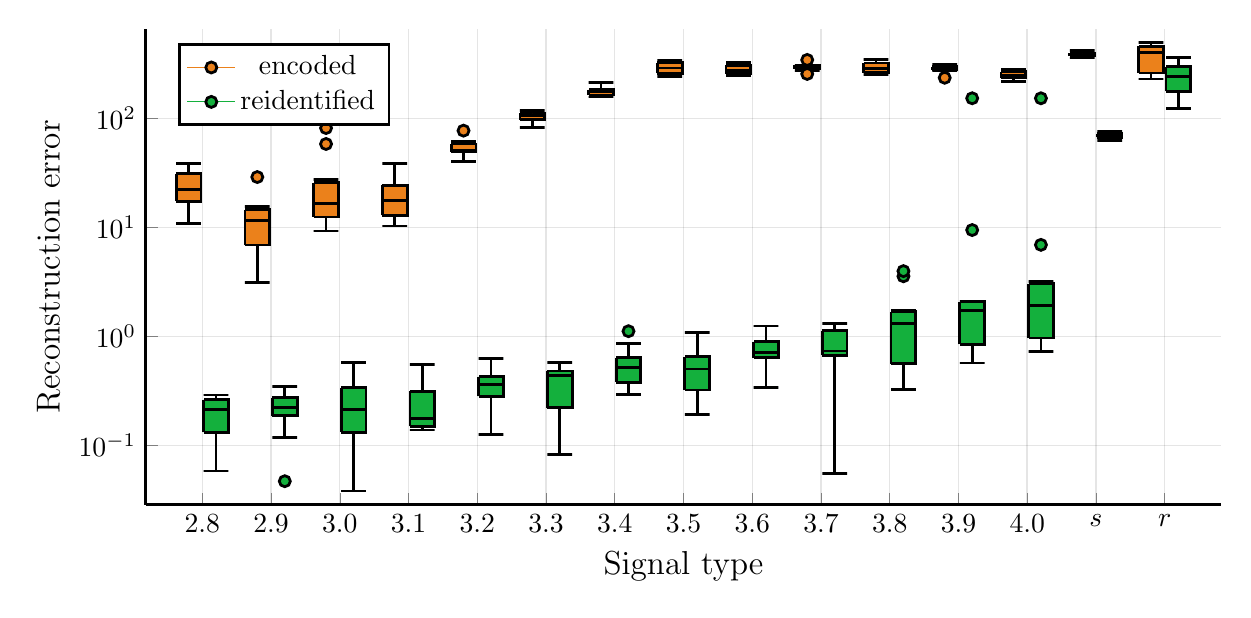
\begin{tikzpicture}[]
\begin{axis}[height = {76.19999999999999mm}, legend pos = {north west}, ylabel = {Reconstruction error}, xmin = {-0.3228}, xmax = {15.322799999999999}, ymax = {662.5170707102975}, ymode = {log}, xlabel = {Signal type}, unbounded coords=jump,scaled x ticks = false,xlabel style = {font = {\fontsize{13 pt}{16.900000000000002 pt}\selectfont}, color = {rgb,1:red,0.00000000;green,0.00000000;blue,0.00000000}, draw opacity = 1.0, rotate = 0.0},xmajorgrids = true,xtick = {0.5,1.5,2.5,3.5,4.5,5.5,6.5,7.5,8.5,9.5,10.5,11.5,12.5,13.5,14.5},xticklabels = {$2.8$,$2.9$,$3.0$,$3.1$,$3.2$,$3.3$,$3.4$,$3.5$,$3.6$,$3.7$,$3.8$,$3.9$,$4.0$,$s$,$r$},xtick align = inside,xticklabel style = {font = {\fontsize{10 pt}{13.0 pt}\selectfont}, color = {rgb,1:red,0.00000000;green,0.00000000;blue,0.00000000}, draw opacity = 1.0, rotate = 0.0},x grid style = {color = {rgb,1:red,0.00000000;green,0.00000000;blue,0.00000000},
draw opacity = 0.1,
line width = 0.5,
solid},axis x line* = left,x axis line style = {color = {rgb,1:red,0.00000000;green,0.00000000;blue,0.00000000},
draw opacity = 1.0,
line width = 1,
solid},scaled y ticks = false,ylabel style = {font = {\fontsize{13 pt}{16.900000000000002 pt}\selectfont}, color = {rgb,1:red,0.00000000;green,0.00000000;blue,0.00000000}, draw opacity = 1.0, rotate = 0.0},log basis y=10,ymajorgrids = true,ytick = {0.1,1.0,10.0,100.0},yticklabels = {$10^{-1}$,$10^{0}$,$10^{1}$,$10^{2}$},ytick align = inside,yticklabel style = {font = {\fontsize{10 pt}{13.0 pt}\selectfont}, color = {rgb,1:red,0.00000000;green,0.00000000;blue,0.00000000}, draw opacity = 1.0, rotate = 0.0},y grid style = {color = {rgb,1:red,0.00000000;green,0.00000000;blue,0.00000000},
draw opacity = 0.1,
line width = 0.5,
solid},axis y line* = left,y axis line style = {color = {rgb,1:red,0.00000000;green,0.00000000;blue,0.00000000},
draw opacity = 1.0,
line width = 1,
solid},    xshift = 0.0mm,
    yshift = 0.0mm,
    axis background/.style={fill={rgb,1:red,1.00000000;green,1.00000000;blue,1.00000000}}
,legend style = {color = {rgb,1:red,0.00000000;green,0.00000000;blue,0.00000000},
draw opacity = 1.0,
line width = 1,
solid,fill = {rgb,1:red,1.00000000;green,1.00000000;blue,1.00000000},font = {\fontsize{10 pt}{13.0 pt}\selectfont}},colorbar style={title=}, ymin = {0.028726737344608507}, width = {152.4mm}]\addplot+[draw=none, color = {rgb,1:red,0.92156863;green,0.50588235;blue,0.10588235},
draw opacity = 1.0,
line width = 0,
solid,mark = *,
mark size = 2.0,
mark options = {
    color = {rgb,1:red,0.00000000;green,0.00000000;blue,0.00000000}, draw opacity = 1.0,
    fill = {rgb,1:red,0.92156863;green,0.50588235;blue,0.10588235}, fill opacity = 1.0,
    line width = 1,
    rotate = 0,
    solid
}] coordinates {
(1.3, 29.055774688720703)
(2.3, 58.43292236328125)
(2.3, 81.81697082519531)
(4.3, 77.44379425048828)
(9.3, 345.1807861328125)
(9.3, 256.5791320800781)
(11.3, 236.64788818359375)
};
\addlegendentry{encoded}
\addlegendentry{reidentified}
\addplot+ [color = {rgb,1:red,0.00000000;green,0.00000000;blue,0.00000000},
draw opacity = 1.0,
line width = 1,
solid,mark = none,
mark size = 2.0,
mark options = {
    color = {rgb,1:red,0.00000000;green,0.00000000;blue,0.00000000}, draw opacity = 1.0,
    fill = {rgb,1:red,0.92156863;green,0.50588235;blue,0.10588235}, fill opacity = 1.0,
    line width = 1,
    rotate = 0,
    solid
},fill = {rgb,1:red,0.92156863;green,0.50588235;blue,0.10588235}, fill opacity=1.0,forget plot]coordinates {
(0.3, 10.867465019226074)
(0.11999999999999997, 10.867465019226074)
(0.48, 10.867465019226074)
(0.3, 10.867465019226074)
(0.3, 17.441078186035156)
};
\addplot+ [color = {rgb,1:red,0.00000000;green,0.00000000;blue,0.00000000},
draw opacity = 1.0,
line width = 1,
solid,mark = none,
mark size = 2.0,
mark options = {
    color = {rgb,1:red,0.00000000;green,0.00000000;blue,0.00000000}, draw opacity = 1.0,
    fill = {rgb,1:red,0.92156863;green,0.50588235;blue,0.10588235}, fill opacity = 1.0,
    line width = 1,
    rotate = 0,
    solid
},fill = {rgb,1:red,0.92156863;green,0.50588235;blue,0.10588235}, fill opacity=1.0,forget plot]coordinates {
(0.11999999999999997, 17.441078186035156)
(0.11999999999999997, 22.494403839111328)
(0.48, 22.494403839111328)
(0.48, 17.441078186035156)
(0.11999999999999997, 17.441078186035156)
};
\addplot+ [color = {rgb,1:red,0.00000000;green,0.00000000;blue,0.00000000},
draw opacity = 1.0,
line width = 1,
solid,mark = none,
mark size = 2.0,
mark options = {
    color = {rgb,1:red,0.00000000;green,0.00000000;blue,0.00000000}, draw opacity = 1.0,
    fill = {rgb,1:red,0.92156863;green,0.50588235;blue,0.10588235}, fill opacity = 1.0,
    line width = 1,
    rotate = 0,
    solid
},fill = {rgb,1:red,0.92156863;green,0.50588235;blue,0.10588235}, fill opacity=1.0,forget plot]coordinates {
(0.11999999999999997, 31.15847873687744)
(0.11999999999999997, 22.494403839111328)
(0.48, 22.494403839111328)
(0.48, 31.15847873687744)
(0.11999999999999997, 31.15847873687744)
};
\addplot+ [color = {rgb,1:red,0.00000000;green,0.00000000;blue,0.00000000},
draw opacity = 1.0,
line width = 1,
solid,mark = none,
mark size = 2.0,
mark options = {
    color = {rgb,1:red,0.00000000;green,0.00000000;blue,0.00000000}, draw opacity = 1.0,
    fill = {rgb,1:red,0.92156863;green,0.50588235;blue,0.10588235}, fill opacity = 1.0,
    line width = 1,
    rotate = 0,
    solid
},fill = {rgb,1:red,0.92156863;green,0.50588235;blue,0.10588235}, fill opacity=1.0,forget plot]coordinates {
(0.3, 38.78556442260742)
(0.11999999999999997, 38.78556442260742)
(0.48, 38.78556442260742)
(0.3, 38.78556442260742)
(0.3, 31.15847873687744)
};
\addplot+ [color = {rgb,1:red,0.00000000;green,0.00000000;blue,0.00000000},
draw opacity = 1.0,
line width = 1,
solid,mark = none,
mark size = 2.0,
mark options = {
    color = {rgb,1:red,0.00000000;green,0.00000000;blue,0.00000000}, draw opacity = 1.0,
    fill = {rgb,1:red,0.92156863;green,0.50588235;blue,0.10588235}, fill opacity = 1.0,
    line width = 1,
    rotate = 0,
    solid
},fill = {rgb,1:red,0.92156863;green,0.50588235;blue,0.10588235}, fill opacity=1.0,forget plot]coordinates {
(1.3, 3.1521103382110596)
(1.12, 3.1521103382110596)
(1.48, 3.1521103382110596)
(1.3, 3.1521103382110596)
(1.3, 6.90257203578949)
};
\addplot+ [color = {rgb,1:red,0.00000000;green,0.00000000;blue,0.00000000},
draw opacity = 1.0,
line width = 1,
solid,mark = none,
mark size = 2.0,
mark options = {
    color = {rgb,1:red,0.00000000;green,0.00000000;blue,0.00000000}, draw opacity = 1.0,
    fill = {rgb,1:red,0.92156863;green,0.50588235;blue,0.10588235}, fill opacity = 1.0,
    line width = 1,
    rotate = 0,
    solid
},fill = {rgb,1:red,0.92156863;green,0.50588235;blue,0.10588235}, fill opacity=1.0,forget plot]coordinates {
(1.12, 6.90257203578949)
(1.12, 11.578704357147217)
(1.48, 11.578704357147217)
(1.48, 6.90257203578949)
(1.12, 6.90257203578949)
};
\addplot+ [color = {rgb,1:red,0.00000000;green,0.00000000;blue,0.00000000},
draw opacity = 1.0,
line width = 1,
solid,mark = none,
mark size = 2.0,
mark options = {
    color = {rgb,1:red,0.00000000;green,0.00000000;blue,0.00000000}, draw opacity = 1.0,
    fill = {rgb,1:red,0.92156863;green,0.50588235;blue,0.10588235}, fill opacity = 1.0,
    line width = 1,
    rotate = 0,
    solid
},fill = {rgb,1:red,0.92156863;green,0.50588235;blue,0.10588235}, fill opacity=1.0,forget plot]coordinates {
(1.12, 14.601720571517944)
(1.12, 11.578704357147217)
(1.48, 11.578704357147217)
(1.48, 14.601720571517944)
(1.12, 14.601720571517944)
};
\addplot+ [color = {rgb,1:red,0.00000000;green,0.00000000;blue,0.00000000},
draw opacity = 1.0,
line width = 1,
solid,mark = none,
mark size = 2.0,
mark options = {
    color = {rgb,1:red,0.00000000;green,0.00000000;blue,0.00000000}, draw opacity = 1.0,
    fill = {rgb,1:red,0.92156863;green,0.50588235;blue,0.10588235}, fill opacity = 1.0,
    line width = 1,
    rotate = 0,
    solid
},fill = {rgb,1:red,0.92156863;green,0.50588235;blue,0.10588235}, fill opacity=1.0,forget plot]coordinates {
(1.3, 15.519279479980469)
(1.12, 15.519279479980469)
(1.48, 15.519279479980469)
(1.3, 15.519279479980469)
(1.3, 14.601720571517944)
};
\addplot+ [color = {rgb,1:red,0.00000000;green,0.00000000;blue,0.00000000},
draw opacity = 1.0,
line width = 1,
solid,mark = none,
mark size = 2.0,
mark options = {
    color = {rgb,1:red,0.00000000;green,0.00000000;blue,0.00000000}, draw opacity = 1.0,
    fill = {rgb,1:red,0.92156863;green,0.50588235;blue,0.10588235}, fill opacity = 1.0,
    line width = 1,
    rotate = 0,
    solid
},fill = {rgb,1:red,0.92156863;green,0.50588235;blue,0.10588235}, fill opacity=1.0,forget plot]coordinates {
(2.3, 9.296589851379395)
(2.1199999999999997, 9.296589851379395)
(2.48, 9.296589851379395)
(2.3, 9.296589851379395)
(2.3, 12.521861553192139)
};
\addplot+ [color = {rgb,1:red,0.00000000;green,0.00000000;blue,0.00000000},
draw opacity = 1.0,
line width = 1,
solid,mark = none,
mark size = 2.0,
mark options = {
    color = {rgb,1:red,0.00000000;green,0.00000000;blue,0.00000000}, draw opacity = 1.0,
    fill = {rgb,1:red,0.92156863;green,0.50588235;blue,0.10588235}, fill opacity = 1.0,
    line width = 1,
    rotate = 0,
    solid
},fill = {rgb,1:red,0.92156863;green,0.50588235;blue,0.10588235}, fill opacity=1.0,forget plot]coordinates {
(2.1199999999999997, 12.521861553192139)
(2.1199999999999997, 16.7490873336792)
(2.48, 16.7490873336792)
(2.48, 12.521861553192139)
(2.1199999999999997, 12.521861553192139)
};
\addplot+ [color = {rgb,1:red,0.00000000;green,0.00000000;blue,0.00000000},
draw opacity = 1.0,
line width = 1,
solid,mark = none,
mark size = 2.0,
mark options = {
    color = {rgb,1:red,0.00000000;green,0.00000000;blue,0.00000000}, draw opacity = 1.0,
    fill = {rgb,1:red,0.92156863;green,0.50588235;blue,0.10588235}, fill opacity = 1.0,
    line width = 1,
    rotate = 0,
    solid
},fill = {rgb,1:red,0.92156863;green,0.50588235;blue,0.10588235}, fill opacity=1.0,forget plot]coordinates {
(2.1199999999999997, 25.8030686378479)
(2.1199999999999997, 16.7490873336792)
(2.48, 16.7490873336792)
(2.48, 25.8030686378479)
(2.1199999999999997, 25.8030686378479)
};
\addplot+ [color = {rgb,1:red,0.00000000;green,0.00000000;blue,0.00000000},
draw opacity = 1.0,
line width = 1,
solid,mark = none,
mark size = 2.0,
mark options = {
    color = {rgb,1:red,0.00000000;green,0.00000000;blue,0.00000000}, draw opacity = 1.0,
    fill = {rgb,1:red,0.92156863;green,0.50588235;blue,0.10588235}, fill opacity = 1.0,
    line width = 1,
    rotate = 0,
    solid
},fill = {rgb,1:red,0.92156863;green,0.50588235;blue,0.10588235}, fill opacity=1.0,forget plot]coordinates {
(2.3, 27.37742805480957)
(2.1199999999999997, 27.37742805480957)
(2.48, 27.37742805480957)
(2.3, 27.37742805480957)
(2.3, 25.8030686378479)
};
\addplot+ [color = {rgb,1:red,0.00000000;green,0.00000000;blue,0.00000000},
draw opacity = 1.0,
line width = 1,
solid,mark = none,
mark size = 2.0,
mark options = {
    color = {rgb,1:red,0.00000000;green,0.00000000;blue,0.00000000}, draw opacity = 1.0,
    fill = {rgb,1:red,0.92156863;green,0.50588235;blue,0.10588235}, fill opacity = 1.0,
    line width = 1,
    rotate = 0,
    solid
},fill = {rgb,1:red,0.92156863;green,0.50588235;blue,0.10588235}, fill opacity=1.0,forget plot]coordinates {
(3.3, 10.342211723327637)
(3.1199999999999997, 10.342211723327637)
(3.48, 10.342211723327637)
(3.3, 10.342211723327637)
(3.3, 12.956748962402344)
};
\addplot+ [color = {rgb,1:red,0.00000000;green,0.00000000;blue,0.00000000},
draw opacity = 1.0,
line width = 1,
solid,mark = none,
mark size = 2.0,
mark options = {
    color = {rgb,1:red,0.00000000;green,0.00000000;blue,0.00000000}, draw opacity = 1.0,
    fill = {rgb,1:red,0.92156863;green,0.50588235;blue,0.10588235}, fill opacity = 1.0,
    line width = 1,
    rotate = 0,
    solid
},fill = {rgb,1:red,0.92156863;green,0.50588235;blue,0.10588235}, fill opacity=1.0,forget plot]coordinates {
(3.1199999999999997, 12.956748962402344)
(3.1199999999999997, 17.761272430419922)
(3.48, 17.761272430419922)
(3.48, 12.956748962402344)
(3.1199999999999997, 12.956748962402344)
};
\addplot+ [color = {rgb,1:red,0.00000000;green,0.00000000;blue,0.00000000},
draw opacity = 1.0,
line width = 1,
solid,mark = none,
mark size = 2.0,
mark options = {
    color = {rgb,1:red,0.00000000;green,0.00000000;blue,0.00000000}, draw opacity = 1.0,
    fill = {rgb,1:red,0.92156863;green,0.50588235;blue,0.10588235}, fill opacity = 1.0,
    line width = 1,
    rotate = 0,
    solid
},fill = {rgb,1:red,0.92156863;green,0.50588235;blue,0.10588235}, fill opacity=1.0,forget plot]coordinates {
(3.1199999999999997, 24.47358751296997)
(3.1199999999999997, 17.761272430419922)
(3.48, 17.761272430419922)
(3.48, 24.47358751296997)
(3.1199999999999997, 24.47358751296997)
};
\addplot+ [color = {rgb,1:red,0.00000000;green,0.00000000;blue,0.00000000},
draw opacity = 1.0,
line width = 1,
solid,mark = none,
mark size = 2.0,
mark options = {
    color = {rgb,1:red,0.00000000;green,0.00000000;blue,0.00000000}, draw opacity = 1.0,
    fill = {rgb,1:red,0.92156863;green,0.50588235;blue,0.10588235}, fill opacity = 1.0,
    line width = 1,
    rotate = 0,
    solid
},fill = {rgb,1:red,0.92156863;green,0.50588235;blue,0.10588235}, fill opacity=1.0,forget plot]coordinates {
(3.3, 38.824127197265625)
(3.1199999999999997, 38.824127197265625)
(3.48, 38.824127197265625)
(3.3, 38.824127197265625)
(3.3, 24.47358751296997)
};
\addplot+ [color = {rgb,1:red,0.00000000;green,0.00000000;blue,0.00000000},
draw opacity = 1.0,
line width = 1,
solid,mark = none,
mark size = 2.0,
mark options = {
    color = {rgb,1:red,0.00000000;green,0.00000000;blue,0.00000000}, draw opacity = 1.0,
    fill = {rgb,1:red,0.92156863;green,0.50588235;blue,0.10588235}, fill opacity = 1.0,
    line width = 1,
    rotate = 0,
    solid
},fill = {rgb,1:red,0.92156863;green,0.50588235;blue,0.10588235}, fill opacity=1.0,forget plot]coordinates {
(4.3, 40.35332107543945)
(4.12, 40.35332107543945)
(4.4799999999999995, 40.35332107543945)
(4.3, 40.35332107543945)
(4.3, 49.50746250152588)
};
\addplot+ [color = {rgb,1:red,0.00000000;green,0.00000000;blue,0.00000000},
draw opacity = 1.0,
line width = 1,
solid,mark = none,
mark size = 2.0,
mark options = {
    color = {rgb,1:red,0.00000000;green,0.00000000;blue,0.00000000}, draw opacity = 1.0,
    fill = {rgb,1:red,0.92156863;green,0.50588235;blue,0.10588235}, fill opacity = 1.0,
    line width = 1,
    rotate = 0,
    solid
},fill = {rgb,1:red,0.92156863;green,0.50588235;blue,0.10588235}, fill opacity=1.0,forget plot]coordinates {
(4.12, 49.50746250152588)
(4.12, 51.022865295410156)
(4.4799999999999995, 51.022865295410156)
(4.4799999999999995, 49.50746250152588)
(4.12, 49.50746250152588)
};
\addplot+ [color = {rgb,1:red,0.00000000;green,0.00000000;blue,0.00000000},
draw opacity = 1.0,
line width = 1,
solid,mark = none,
mark size = 2.0,
mark options = {
    color = {rgb,1:red,0.00000000;green,0.00000000;blue,0.00000000}, draw opacity = 1.0,
    fill = {rgb,1:red,0.92156863;green,0.50588235;blue,0.10588235}, fill opacity = 1.0,
    line width = 1,
    rotate = 0,
    solid
},fill = {rgb,1:red,0.92156863;green,0.50588235;blue,0.10588235}, fill opacity=1.0,forget plot]coordinates {
(4.12, 58.51133346557617)
(4.12, 51.022865295410156)
(4.4799999999999995, 51.022865295410156)
(4.4799999999999995, 58.51133346557617)
(4.12, 58.51133346557617)
};
\addplot+ [color = {rgb,1:red,0.00000000;green,0.00000000;blue,0.00000000},
draw opacity = 1.0,
line width = 1,
solid,mark = none,
mark size = 2.0,
mark options = {
    color = {rgb,1:red,0.00000000;green,0.00000000;blue,0.00000000}, draw opacity = 1.0,
    fill = {rgb,1:red,0.92156863;green,0.50588235;blue,0.10588235}, fill opacity = 1.0,
    line width = 1,
    rotate = 0,
    solid
},fill = {rgb,1:red,0.92156863;green,0.50588235;blue,0.10588235}, fill opacity=1.0,forget plot]coordinates {
(4.3, 61.58100891113281)
(4.12, 61.58100891113281)
(4.4799999999999995, 61.58100891113281)
(4.3, 61.58100891113281)
(4.3, 58.51133346557617)
};
\addplot+ [color = {rgb,1:red,0.00000000;green,0.00000000;blue,0.00000000},
draw opacity = 1.0,
line width = 1,
solid,mark = none,
mark size = 2.0,
mark options = {
    color = {rgb,1:red,0.00000000;green,0.00000000;blue,0.00000000}, draw opacity = 1.0,
    fill = {rgb,1:red,0.92156863;green,0.50588235;blue,0.10588235}, fill opacity = 1.0,
    line width = 1,
    rotate = 0,
    solid
},fill = {rgb,1:red,0.92156863;green,0.50588235;blue,0.10588235}, fill opacity=1.0,forget plot]coordinates {
(5.3, 82.34829711914062)
(5.12, 82.34829711914062)
(5.4799999999999995, 82.34829711914062)
(5.3, 82.34829711914062)
(5.3, 97.81059837341309)
};
\addplot+ [color = {rgb,1:red,0.00000000;green,0.00000000;blue,0.00000000},
draw opacity = 1.0,
line width = 1,
solid,mark = none,
mark size = 2.0,
mark options = {
    color = {rgb,1:red,0.00000000;green,0.00000000;blue,0.00000000}, draw opacity = 1.0,
    fill = {rgb,1:red,0.92156863;green,0.50588235;blue,0.10588235}, fill opacity = 1.0,
    line width = 1,
    rotate = 0,
    solid
},fill = {rgb,1:red,0.92156863;green,0.50588235;blue,0.10588235}, fill opacity=1.0,forget plot]coordinates {
(5.12, 97.81059837341309)
(5.12, 106.15861129760742)
(5.4799999999999995, 106.15861129760742)
(5.4799999999999995, 97.81059837341309)
(5.12, 97.81059837341309)
};
\addplot+ [color = {rgb,1:red,0.00000000;green,0.00000000;blue,0.00000000},
draw opacity = 1.0,
line width = 1,
solid,mark = none,
mark size = 2.0,
mark options = {
    color = {rgb,1:red,0.00000000;green,0.00000000;blue,0.00000000}, draw opacity = 1.0,
    fill = {rgb,1:red,0.92156863;green,0.50588235;blue,0.10588235}, fill opacity = 1.0,
    line width = 1,
    rotate = 0,
    solid
},fill = {rgb,1:red,0.92156863;green,0.50588235;blue,0.10588235}, fill opacity=1.0,forget plot]coordinates {
(5.12, 111.30532264709473)
(5.12, 106.15861129760742)
(5.4799999999999995, 106.15861129760742)
(5.4799999999999995, 111.30532264709473)
(5.12, 111.30532264709473)
};
\addplot+ [color = {rgb,1:red,0.00000000;green,0.00000000;blue,0.00000000},
draw opacity = 1.0,
line width = 1,
solid,mark = none,
mark size = 2.0,
mark options = {
    color = {rgb,1:red,0.00000000;green,0.00000000;blue,0.00000000}, draw opacity = 1.0,
    fill = {rgb,1:red,0.92156863;green,0.50588235;blue,0.10588235}, fill opacity = 1.0,
    line width = 1,
    rotate = 0,
    solid
},fill = {rgb,1:red,0.92156863;green,0.50588235;blue,0.10588235}, fill opacity=1.0,forget plot]coordinates {
(5.3, 118.78929138183594)
(5.12, 118.78929138183594)
(5.4799999999999995, 118.78929138183594)
(5.3, 118.78929138183594)
(5.3, 111.30532264709473)
};
\addplot+ [color = {rgb,1:red,0.00000000;green,0.00000000;blue,0.00000000},
draw opacity = 1.0,
line width = 1,
solid,mark = none,
mark size = 2.0,
mark options = {
    color = {rgb,1:red,0.00000000;green,0.00000000;blue,0.00000000}, draw opacity = 1.0,
    fill = {rgb,1:red,0.92156863;green,0.50588235;blue,0.10588235}, fill opacity = 1.0,
    line width = 1,
    rotate = 0,
    solid
},fill = {rgb,1:red,0.92156863;green,0.50588235;blue,0.10588235}, fill opacity=1.0,forget plot]coordinates {
(6.3, 157.7874298095703)
(6.12, 157.7874298095703)
(6.4799999999999995, 157.7874298095703)
(6.3, 157.7874298095703)
(6.3, 164.21955108642578)
};
\addplot+ [color = {rgb,1:red,0.00000000;green,0.00000000;blue,0.00000000},
draw opacity = 1.0,
line width = 1,
solid,mark = none,
mark size = 2.0,
mark options = {
    color = {rgb,1:red,0.00000000;green,0.00000000;blue,0.00000000}, draw opacity = 1.0,
    fill = {rgb,1:red,0.92156863;green,0.50588235;blue,0.10588235}, fill opacity = 1.0,
    line width = 1,
    rotate = 0,
    solid
},fill = {rgb,1:red,0.92156863;green,0.50588235;blue,0.10588235}, fill opacity=1.0,forget plot]coordinates {
(6.12, 164.21955108642578)
(6.12, 177.64422607421875)
(6.4799999999999995, 177.64422607421875)
(6.4799999999999995, 164.21955108642578)
(6.12, 164.21955108642578)
};
\addplot+ [color = {rgb,1:red,0.00000000;green,0.00000000;blue,0.00000000},
draw opacity = 1.0,
line width = 1,
solid,mark = none,
mark size = 2.0,
mark options = {
    color = {rgb,1:red,0.00000000;green,0.00000000;blue,0.00000000}, draw opacity = 1.0,
    fill = {rgb,1:red,0.92156863;green,0.50588235;blue,0.10588235}, fill opacity = 1.0,
    line width = 1,
    rotate = 0,
    solid
},fill = {rgb,1:red,0.92156863;green,0.50588235;blue,0.10588235}, fill opacity=1.0,forget plot]coordinates {
(6.12, 184.19443130493164)
(6.12, 177.64422607421875)
(6.4799999999999995, 177.64422607421875)
(6.4799999999999995, 184.19443130493164)
(6.12, 184.19443130493164)
};
\addplot+ [color = {rgb,1:red,0.00000000;green,0.00000000;blue,0.00000000},
draw opacity = 1.0,
line width = 1,
solid,mark = none,
mark size = 2.0,
mark options = {
    color = {rgb,1:red,0.00000000;green,0.00000000;blue,0.00000000}, draw opacity = 1.0,
    fill = {rgb,1:red,0.92156863;green,0.50588235;blue,0.10588235}, fill opacity = 1.0,
    line width = 1,
    rotate = 0,
    solid
},fill = {rgb,1:red,0.92156863;green,0.50588235;blue,0.10588235}, fill opacity=1.0,forget plot]coordinates {
(6.3, 213.3422088623047)
(6.12, 213.3422088623047)
(6.4799999999999995, 213.3422088623047)
(6.3, 213.3422088623047)
(6.3, 184.19443130493164)
};
\addplot+ [color = {rgb,1:red,0.00000000;green,0.00000000;blue,0.00000000},
draw opacity = 1.0,
line width = 1,
solid,mark = none,
mark size = 2.0,
mark options = {
    color = {rgb,1:red,0.00000000;green,0.00000000;blue,0.00000000}, draw opacity = 1.0,
    fill = {rgb,1:red,0.92156863;green,0.50588235;blue,0.10588235}, fill opacity = 1.0,
    line width = 1,
    rotate = 0,
    solid
},fill = {rgb,1:red,0.92156863;green,0.50588235;blue,0.10588235}, fill opacity=1.0,forget plot]coordinates {
(7.3, 243.187255859375)
(7.12, 243.187255859375)
(7.4799999999999995, 243.187255859375)
(7.3, 243.187255859375)
(7.3, 259.30875396728516)
};
\addplot+ [color = {rgb,1:red,0.00000000;green,0.00000000;blue,0.00000000},
draw opacity = 1.0,
line width = 1,
solid,mark = none,
mark size = 2.0,
mark options = {
    color = {rgb,1:red,0.00000000;green,0.00000000;blue,0.00000000}, draw opacity = 1.0,
    fill = {rgb,1:red,0.92156863;green,0.50588235;blue,0.10588235}, fill opacity = 1.0,
    line width = 1,
    rotate = 0,
    solid
},fill = {rgb,1:red,0.92156863;green,0.50588235;blue,0.10588235}, fill opacity=1.0,forget plot]coordinates {
(7.12, 259.30875396728516)
(7.12, 291.3841094970703)
(7.4799999999999995, 291.3841094970703)
(7.4799999999999995, 259.30875396728516)
(7.12, 259.30875396728516)
};
\addplot+ [color = {rgb,1:red,0.00000000;green,0.00000000;blue,0.00000000},
draw opacity = 1.0,
line width = 1,
solid,mark = none,
mark size = 2.0,
mark options = {
    color = {rgb,1:red,0.00000000;green,0.00000000;blue,0.00000000}, draw opacity = 1.0,
    fill = {rgb,1:red,0.92156863;green,0.50588235;blue,0.10588235}, fill opacity = 1.0,
    line width = 1,
    rotate = 0,
    solid
},fill = {rgb,1:red,0.92156863;green,0.50588235;blue,0.10588235}, fill opacity=1.0,forget plot]coordinates {
(7.12, 326.21466064453125)
(7.12, 291.3841094970703)
(7.4799999999999995, 291.3841094970703)
(7.4799999999999995, 326.21466064453125)
(7.12, 326.21466064453125)
};
\addplot+ [color = {rgb,1:red,0.00000000;green,0.00000000;blue,0.00000000},
draw opacity = 1.0,
line width = 1,
solid,mark = none,
mark size = 2.0,
mark options = {
    color = {rgb,1:red,0.00000000;green,0.00000000;blue,0.00000000}, draw opacity = 1.0,
    fill = {rgb,1:red,0.92156863;green,0.50588235;blue,0.10588235}, fill opacity = 1.0,
    line width = 1,
    rotate = 0,
    solid
},fill = {rgb,1:red,0.92156863;green,0.50588235;blue,0.10588235}, fill opacity=1.0,forget plot]coordinates {
(7.3, 340.9198913574219)
(7.12, 340.9198913574219)
(7.4799999999999995, 340.9198913574219)
(7.3, 340.9198913574219)
(7.3, 326.21466064453125)
};
\addplot+ [color = {rgb,1:red,0.00000000;green,0.00000000;blue,0.00000000},
draw opacity = 1.0,
line width = 1,
solid,mark = none,
mark size = 2.0,
mark options = {
    color = {rgb,1:red,0.00000000;green,0.00000000;blue,0.00000000}, draw opacity = 1.0,
    fill = {rgb,1:red,0.92156863;green,0.50588235;blue,0.10588235}, fill opacity = 1.0,
    line width = 1,
    rotate = 0,
    solid
},fill = {rgb,1:red,0.92156863;green,0.50588235;blue,0.10588235}, fill opacity=1.0,forget plot]coordinates {
(8.3, 249.42568969726562)
(8.120000000000001, 249.42568969726562)
(8.48, 249.42568969726562)
(8.3, 249.42568969726562)
(8.3, 258.3868942260742)
};
\addplot+ [color = {rgb,1:red,0.00000000;green,0.00000000;blue,0.00000000},
draw opacity = 1.0,
line width = 1,
solid,mark = none,
mark size = 2.0,
mark options = {
    color = {rgb,1:red,0.00000000;green,0.00000000;blue,0.00000000}, draw opacity = 1.0,
    fill = {rgb,1:red,0.92156863;green,0.50588235;blue,0.10588235}, fill opacity = 1.0,
    line width = 1,
    rotate = 0,
    solid
},fill = {rgb,1:red,0.92156863;green,0.50588235;blue,0.10588235}, fill opacity=1.0,forget plot]coordinates {
(8.120000000000001, 258.3868942260742)
(8.120000000000001, 275.39857482910156)
(8.48, 275.39857482910156)
(8.48, 258.3868942260742)
(8.120000000000001, 258.3868942260742)
};
\addplot+ [color = {rgb,1:red,0.00000000;green,0.00000000;blue,0.00000000},
draw opacity = 1.0,
line width = 1,
solid,mark = none,
mark size = 2.0,
mark options = {
    color = {rgb,1:red,0.00000000;green,0.00000000;blue,0.00000000}, draw opacity = 1.0,
    fill = {rgb,1:red,0.92156863;green,0.50588235;blue,0.10588235}, fill opacity = 1.0,
    line width = 1,
    rotate = 0,
    solid
},fill = {rgb,1:red,0.92156863;green,0.50588235;blue,0.10588235}, fill opacity=1.0,forget plot]coordinates {
(8.120000000000001, 307.469970703125)
(8.120000000000001, 275.39857482910156)
(8.48, 275.39857482910156)
(8.48, 307.469970703125)
(8.120000000000001, 307.469970703125)
};
\addplot+ [color = {rgb,1:red,0.00000000;green,0.00000000;blue,0.00000000},
draw opacity = 1.0,
line width = 1,
solid,mark = none,
mark size = 2.0,
mark options = {
    color = {rgb,1:red,0.00000000;green,0.00000000;blue,0.00000000}, draw opacity = 1.0,
    fill = {rgb,1:red,0.92156863;green,0.50588235;blue,0.10588235}, fill opacity = 1.0,
    line width = 1,
    rotate = 0,
    solid
},fill = {rgb,1:red,0.92156863;green,0.50588235;blue,0.10588235}, fill opacity=1.0,forget plot]coordinates {
(8.3, 324.40301513671875)
(8.120000000000001, 324.40301513671875)
(8.48, 324.40301513671875)
(8.3, 324.40301513671875)
(8.3, 307.469970703125)
};
\addplot+ [color = {rgb,1:red,0.00000000;green,0.00000000;blue,0.00000000},
draw opacity = 1.0,
line width = 1,
solid,mark = none,
mark size = 2.0,
mark options = {
    color = {rgb,1:red,0.00000000;green,0.00000000;blue,0.00000000}, draw opacity = 1.0,
    fill = {rgb,1:red,0.92156863;green,0.50588235;blue,0.10588235}, fill opacity = 1.0,
    line width = 1,
    rotate = 0,
    solid
},fill = {rgb,1:red,0.92156863;green,0.50588235;blue,0.10588235}, fill opacity=1.0,forget plot]coordinates {
(9.3, 275.405517578125)
(9.120000000000001, 275.405517578125)
(9.48, 275.405517578125)
(9.3, 275.405517578125)
(9.3, 288.12052154541016)
};
\addplot+ [color = {rgb,1:red,0.00000000;green,0.00000000;blue,0.00000000},
draw opacity = 1.0,
line width = 1,
solid,mark = none,
mark size = 2.0,
mark options = {
    color = {rgb,1:red,0.00000000;green,0.00000000;blue,0.00000000}, draw opacity = 1.0,
    fill = {rgb,1:red,0.92156863;green,0.50588235;blue,0.10588235}, fill opacity = 1.0,
    line width = 1,
    rotate = 0,
    solid
},fill = {rgb,1:red,0.92156863;green,0.50588235;blue,0.10588235}, fill opacity=1.0,forget plot]coordinates {
(9.120000000000001, 288.12052154541016)
(9.120000000000001, 295.4416046142578)
(9.48, 295.4416046142578)
(9.48, 288.12052154541016)
(9.120000000000001, 288.12052154541016)
};
\addplot+ [color = {rgb,1:red,0.00000000;green,0.00000000;blue,0.00000000},
draw opacity = 1.0,
line width = 1,
solid,mark = none,
mark size = 2.0,
mark options = {
    color = {rgb,1:red,0.00000000;green,0.00000000;blue,0.00000000}, draw opacity = 1.0,
    fill = {rgb,1:red,0.92156863;green,0.50588235;blue,0.10588235}, fill opacity = 1.0,
    line width = 1,
    rotate = 0,
    solid
},fill = {rgb,1:red,0.92156863;green,0.50588235;blue,0.10588235}, fill opacity=1.0,forget plot]coordinates {
(9.120000000000001, 308.7365417480469)
(9.120000000000001, 295.4416046142578)
(9.48, 295.4416046142578)
(9.48, 308.7365417480469)
(9.120000000000001, 308.7365417480469)
};
\addplot+ [color = {rgb,1:red,0.00000000;green,0.00000000;blue,0.00000000},
draw opacity = 1.0,
line width = 1,
solid,mark = none,
mark size = 2.0,
mark options = {
    color = {rgb,1:red,0.00000000;green,0.00000000;blue,0.00000000}, draw opacity = 1.0,
    fill = {rgb,1:red,0.92156863;green,0.50588235;blue,0.10588235}, fill opacity = 1.0,
    line width = 1,
    rotate = 0,
    solid
},fill = {rgb,1:red,0.92156863;green,0.50588235;blue,0.10588235}, fill opacity=1.0,forget plot]coordinates {
(9.3, 310.21502685546875)
(9.120000000000001, 310.21502685546875)
(9.48, 310.21502685546875)
(9.3, 310.21502685546875)
(9.3, 308.7365417480469)
};
\addplot+ [color = {rgb,1:red,0.00000000;green,0.00000000;blue,0.00000000},
draw opacity = 1.0,
line width = 1,
solid,mark = none,
mark size = 2.0,
mark options = {
    color = {rgb,1:red,0.00000000;green,0.00000000;blue,0.00000000}, draw opacity = 1.0,
    fill = {rgb,1:red,0.92156863;green,0.50588235;blue,0.10588235}, fill opacity = 1.0,
    line width = 1,
    rotate = 0,
    solid
},fill = {rgb,1:red,0.92156863;green,0.50588235;blue,0.10588235}, fill opacity=1.0,forget plot]coordinates {
(10.3, 252.637939453125)
(10.120000000000001, 252.637939453125)
(10.48, 252.637939453125)
(10.3, 252.637939453125)
(10.3, 263.6750259399414)
};
\addplot+ [color = {rgb,1:red,0.00000000;green,0.00000000;blue,0.00000000},
draw opacity = 1.0,
line width = 1,
solid,mark = none,
mark size = 2.0,
mark options = {
    color = {rgb,1:red,0.00000000;green,0.00000000;blue,0.00000000}, draw opacity = 1.0,
    fill = {rgb,1:red,0.92156863;green,0.50588235;blue,0.10588235}, fill opacity = 1.0,
    line width = 1,
    rotate = 0,
    solid
},fill = {rgb,1:red,0.92156863;green,0.50588235;blue,0.10588235}, fill opacity=1.0,forget plot]coordinates {
(10.120000000000001, 263.6750259399414)
(10.120000000000001, 288.7881774902344)
(10.48, 288.7881774902344)
(10.48, 263.6750259399414)
(10.120000000000001, 263.6750259399414)
};
\addplot+ [color = {rgb,1:red,0.00000000;green,0.00000000;blue,0.00000000},
draw opacity = 1.0,
line width = 1,
solid,mark = none,
mark size = 2.0,
mark options = {
    color = {rgb,1:red,0.00000000;green,0.00000000;blue,0.00000000}, draw opacity = 1.0,
    fill = {rgb,1:red,0.92156863;green,0.50588235;blue,0.10588235}, fill opacity = 1.0,
    line width = 1,
    rotate = 0,
    solid
},fill = {rgb,1:red,0.92156863;green,0.50588235;blue,0.10588235}, fill opacity=1.0,forget plot]coordinates {
(10.120000000000001, 322.8680419921875)
(10.120000000000001, 288.7881774902344)
(10.48, 288.7881774902344)
(10.48, 322.8680419921875)
(10.120000000000001, 322.8680419921875)
};
\addplot+ [color = {rgb,1:red,0.00000000;green,0.00000000;blue,0.00000000},
draw opacity = 1.0,
line width = 1,
solid,mark = none,
mark size = 2.0,
mark options = {
    color = {rgb,1:red,0.00000000;green,0.00000000;blue,0.00000000}, draw opacity = 1.0,
    fill = {rgb,1:red,0.92156863;green,0.50588235;blue,0.10588235}, fill opacity = 1.0,
    line width = 1,
    rotate = 0,
    solid
},fill = {rgb,1:red,0.92156863;green,0.50588235;blue,0.10588235}, fill opacity=1.0,forget plot]coordinates {
(10.3, 348.84808349609375)
(10.120000000000001, 348.84808349609375)
(10.48, 348.84808349609375)
(10.3, 348.84808349609375)
(10.3, 322.8680419921875)
};
\addplot+ [color = {rgb,1:red,0.00000000;green,0.00000000;blue,0.00000000},
draw opacity = 1.0,
line width = 1,
solid,mark = none,
mark size = 2.0,
mark options = {
    color = {rgb,1:red,0.00000000;green,0.00000000;blue,0.00000000}, draw opacity = 1.0,
    fill = {rgb,1:red,0.92156863;green,0.50588235;blue,0.10588235}, fill opacity = 1.0,
    line width = 1,
    rotate = 0,
    solid
},fill = {rgb,1:red,0.92156863;green,0.50588235;blue,0.10588235}, fill opacity=1.0,forget plot]coordinates {
(11.3, 274.5265808105469)
(11.120000000000001, 274.5265808105469)
(11.48, 274.5265808105469)
(11.3, 274.5265808105469)
(11.3, 279.8248825073242)
};
\addplot+ [color = {rgb,1:red,0.00000000;green,0.00000000;blue,0.00000000},
draw opacity = 1.0,
line width = 1,
solid,mark = none,
mark size = 2.0,
mark options = {
    color = {rgb,1:red,0.00000000;green,0.00000000;blue,0.00000000}, draw opacity = 1.0,
    fill = {rgb,1:red,0.92156863;green,0.50588235;blue,0.10588235}, fill opacity = 1.0,
    line width = 1,
    rotate = 0,
    solid
},fill = {rgb,1:red,0.92156863;green,0.50588235;blue,0.10588235}, fill opacity=1.0,forget plot]coordinates {
(11.120000000000001, 279.8248825073242)
(11.120000000000001, 285.75177001953125)
(11.48, 285.75177001953125)
(11.48, 279.8248825073242)
(11.120000000000001, 279.8248825073242)
};
\addplot+ [color = {rgb,1:red,0.00000000;green,0.00000000;blue,0.00000000},
draw opacity = 1.0,
line width = 1,
solid,mark = none,
mark size = 2.0,
mark options = {
    color = {rgb,1:red,0.00000000;green,0.00000000;blue,0.00000000}, draw opacity = 1.0,
    fill = {rgb,1:red,0.92156863;green,0.50588235;blue,0.10588235}, fill opacity = 1.0,
    line width = 1,
    rotate = 0,
    solid
},fill = {rgb,1:red,0.92156863;green,0.50588235;blue,0.10588235}, fill opacity=1.0,forget plot]coordinates {
(11.120000000000001, 299.6744689941406)
(11.120000000000001, 285.75177001953125)
(11.48, 285.75177001953125)
(11.48, 299.6744689941406)
(11.120000000000001, 299.6744689941406)
};
\addplot+ [color = {rgb,1:red,0.00000000;green,0.00000000;blue,0.00000000},
draw opacity = 1.0,
line width = 1,
solid,mark = none,
mark size = 2.0,
mark options = {
    color = {rgb,1:red,0.00000000;green,0.00000000;blue,0.00000000}, draw opacity = 1.0,
    fill = {rgb,1:red,0.92156863;green,0.50588235;blue,0.10588235}, fill opacity = 1.0,
    line width = 1,
    rotate = 0,
    solid
},fill = {rgb,1:red,0.92156863;green,0.50588235;blue,0.10588235}, fill opacity=1.0,forget plot]coordinates {
(11.3, 313.4098815917969)
(11.120000000000001, 313.4098815917969)
(11.48, 313.4098815917969)
(11.3, 313.4098815917969)
(11.3, 299.6744689941406)
};
\addplot+ [color = {rgb,1:red,0.00000000;green,0.00000000;blue,0.00000000},
draw opacity = 1.0,
line width = 1,
solid,mark = none,
mark size = 2.0,
mark options = {
    color = {rgb,1:red,0.00000000;green,0.00000000;blue,0.00000000}, draw opacity = 1.0,
    fill = {rgb,1:red,0.92156863;green,0.50588235;blue,0.10588235}, fill opacity = 1.0,
    line width = 1,
    rotate = 0,
    solid
},fill = {rgb,1:red,0.92156863;green,0.50588235;blue,0.10588235}, fill opacity=1.0,forget plot]coordinates {
(12.3, 220.34805297851562)
(12.120000000000001, 220.34805297851562)
(12.48, 220.34805297851562)
(12.3, 220.34805297851562)
(12.3, 235.1759147644043)
};
\addplot+ [color = {rgb,1:red,0.00000000;green,0.00000000;blue,0.00000000},
draw opacity = 1.0,
line width = 1,
solid,mark = none,
mark size = 2.0,
mark options = {
    color = {rgb,1:red,0.00000000;green,0.00000000;blue,0.00000000}, draw opacity = 1.0,
    fill = {rgb,1:red,0.92156863;green,0.50588235;blue,0.10588235}, fill opacity = 1.0,
    line width = 1,
    rotate = 0,
    solid
},fill = {rgb,1:red,0.92156863;green,0.50588235;blue,0.10588235}, fill opacity=1.0,forget plot]coordinates {
(12.120000000000001, 235.1759147644043)
(12.120000000000001, 249.46733856201172)
(12.48, 249.46733856201172)
(12.48, 235.1759147644043)
(12.120000000000001, 235.1759147644043)
};
\addplot+ [color = {rgb,1:red,0.00000000;green,0.00000000;blue,0.00000000},
draw opacity = 1.0,
line width = 1,
solid,mark = none,
mark size = 2.0,
mark options = {
    color = {rgb,1:red,0.00000000;green,0.00000000;blue,0.00000000}, draw opacity = 1.0,
    fill = {rgb,1:red,0.92156863;green,0.50588235;blue,0.10588235}, fill opacity = 1.0,
    line width = 1,
    rotate = 0,
    solid
},fill = {rgb,1:red,0.92156863;green,0.50588235;blue,0.10588235}, fill opacity=1.0,forget plot]coordinates {
(12.120000000000001, 268.2483673095703)
(12.120000000000001, 249.46733856201172)
(12.48, 249.46733856201172)
(12.48, 268.2483673095703)
(12.120000000000001, 268.2483673095703)
};
\addplot+ [color = {rgb,1:red,0.00000000;green,0.00000000;blue,0.00000000},
draw opacity = 1.0,
line width = 1,
solid,mark = none,
mark size = 2.0,
mark options = {
    color = {rgb,1:red,0.00000000;green,0.00000000;blue,0.00000000}, draw opacity = 1.0,
    fill = {rgb,1:red,0.92156863;green,0.50588235;blue,0.10588235}, fill opacity = 1.0,
    line width = 1,
    rotate = 0,
    solid
},fill = {rgb,1:red,0.92156863;green,0.50588235;blue,0.10588235}, fill opacity=1.0,forget plot]coordinates {
(12.3, 280.2359619140625)
(12.120000000000001, 280.2359619140625)
(12.48, 280.2359619140625)
(12.3, 280.2359619140625)
(12.3, 268.2483673095703)
};
\addplot+ [color = {rgb,1:red,0.00000000;green,0.00000000;blue,0.00000000},
draw opacity = 1.0,
line width = 1,
solid,mark = none,
mark size = 2.0,
mark options = {
    color = {rgb,1:red,0.00000000;green,0.00000000;blue,0.00000000}, draw opacity = 1.0,
    fill = {rgb,1:red,0.92156863;green,0.50588235;blue,0.10588235}, fill opacity = 1.0,
    line width = 1,
    rotate = 0,
    solid
},fill = {rgb,1:red,0.92156863;green,0.50588235;blue,0.10588235}, fill opacity=1.0,forget plot]coordinates {
(13.3, 360.0884094238281)
(13.120000000000001, 360.0884094238281)
(13.48, 360.0884094238281)
(13.3, 360.0884094238281)
(13.3, 374.8258056640625)
};
\addplot+ [color = {rgb,1:red,0.00000000;green,0.00000000;blue,0.00000000},
draw opacity = 1.0,
line width = 1,
solid,mark = none,
mark size = 2.0,
mark options = {
    color = {rgb,1:red,0.00000000;green,0.00000000;blue,0.00000000}, draw opacity = 1.0,
    fill = {rgb,1:red,0.92156863;green,0.50588235;blue,0.10588235}, fill opacity = 1.0,
    line width = 1,
    rotate = 0,
    solid
},fill = {rgb,1:red,0.92156863;green,0.50588235;blue,0.10588235}, fill opacity=1.0,forget plot]coordinates {
(13.120000000000001, 374.8258056640625)
(13.120000000000001, 384.53321838378906)
(13.48, 384.53321838378906)
(13.48, 374.8258056640625)
(13.120000000000001, 374.8258056640625)
};
\addplot+ [color = {rgb,1:red,0.00000000;green,0.00000000;blue,0.00000000},
draw opacity = 1.0,
line width = 1,
solid,mark = none,
mark size = 2.0,
mark options = {
    color = {rgb,1:red,0.00000000;green,0.00000000;blue,0.00000000}, draw opacity = 1.0,
    fill = {rgb,1:red,0.92156863;green,0.50588235;blue,0.10588235}, fill opacity = 1.0,
    line width = 1,
    rotate = 0,
    solid
},fill = {rgb,1:red,0.92156863;green,0.50588235;blue,0.10588235}, fill opacity=1.0,forget plot]coordinates {
(13.120000000000001, 399.0635299682617)
(13.120000000000001, 384.53321838378906)
(13.48, 384.53321838378906)
(13.48, 399.0635299682617)
(13.120000000000001, 399.0635299682617)
};
\addplot+ [color = {rgb,1:red,0.00000000;green,0.00000000;blue,0.00000000},
draw opacity = 1.0,
line width = 1,
solid,mark = none,
mark size = 2.0,
mark options = {
    color = {rgb,1:red,0.00000000;green,0.00000000;blue,0.00000000}, draw opacity = 1.0,
    fill = {rgb,1:red,0.92156863;green,0.50588235;blue,0.10588235}, fill opacity = 1.0,
    line width = 1,
    rotate = 0,
    solid
},fill = {rgb,1:red,0.92156863;green,0.50588235;blue,0.10588235}, fill opacity=1.0,forget plot]coordinates {
(13.3, 422.36566162109375)
(13.120000000000001, 422.36566162109375)
(13.48, 422.36566162109375)
(13.3, 422.36566162109375)
(13.3, 399.0635299682617)
};
\addplot+ [color = {rgb,1:red,0.00000000;green,0.00000000;blue,0.00000000},
draw opacity = 1.0,
line width = 1,
solid,mark = none,
mark size = 2.0,
mark options = {
    color = {rgb,1:red,0.00000000;green,0.00000000;blue,0.00000000}, draw opacity = 1.0,
    fill = {rgb,1:red,0.92156863;green,0.50588235;blue,0.10588235}, fill opacity = 1.0,
    line width = 1,
    rotate = 0,
    solid
},fill = {rgb,1:red,0.92156863;green,0.50588235;blue,0.10588235}, fill opacity=1.0,forget plot]coordinates {
(14.3, 230.55941772460938)
(14.120000000000001, 230.55941772460938)
(14.48, 230.55941772460938)
(14.3, 230.55941772460938)
(14.3, 261.64928817749023)
};
\addplot+ [color = {rgb,1:red,0.00000000;green,0.00000000;blue,0.00000000},
draw opacity = 1.0,
line width = 1,
solid,mark = none,
mark size = 2.0,
mark options = {
    color = {rgb,1:red,0.00000000;green,0.00000000;blue,0.00000000}, draw opacity = 1.0,
    fill = {rgb,1:red,0.92156863;green,0.50588235;blue,0.10588235}, fill opacity = 1.0,
    line width = 1,
    rotate = 0,
    solid
},fill = {rgb,1:red,0.92156863;green,0.50588235;blue,0.10588235}, fill opacity=1.0,forget plot]coordinates {
(14.120000000000001, 261.64928817749023)
(14.120000000000001, 406.4973602294922)
(14.48, 406.4973602294922)
(14.48, 261.64928817749023)
(14.120000000000001, 261.64928817749023)
};
\addplot+ [color = {rgb,1:red,0.00000000;green,0.00000000;blue,0.00000000},
draw opacity = 1.0,
line width = 1,
solid,mark = none,
mark size = 2.0,
mark options = {
    color = {rgb,1:red,0.00000000;green,0.00000000;blue,0.00000000}, draw opacity = 1.0,
    fill = {rgb,1:red,0.92156863;green,0.50588235;blue,0.10588235}, fill opacity = 1.0,
    line width = 1,
    rotate = 0,
    solid
},fill = {rgb,1:red,0.92156863;green,0.50588235;blue,0.10588235}, fill opacity=1.0,forget plot]coordinates {
(14.120000000000001, 460.04891204833984)
(14.120000000000001, 406.4973602294922)
(14.48, 406.4973602294922)
(14.48, 460.04891204833984)
(14.120000000000001, 460.04891204833984)
};
\addplot+ [color = {rgb,1:red,0.00000000;green,0.00000000;blue,0.00000000},
draw opacity = 1.0,
line width = 1,
solid,mark = none,
mark size = 2.0,
mark options = {
    color = {rgb,1:red,0.00000000;green,0.00000000;blue,0.00000000}, draw opacity = 1.0,
    fill = {rgb,1:red,0.92156863;green,0.50588235;blue,0.10588235}, fill opacity = 1.0,
    line width = 1,
    rotate = 0,
    solid
},fill = {rgb,1:red,0.92156863;green,0.50588235;blue,0.10588235}, fill opacity=1.0,forget plot]coordinates {
(14.3, 498.5611877441406)
(14.120000000000001, 498.5611877441406)
(14.48, 498.5611877441406)
(14.3, 498.5611877441406)
(14.3, 460.04891204833984)
};
\addplot+[draw=none, color = {rgb,1:red,0.07843137;green,0.69019608;blue,0.23921569},
draw opacity = 1.0,
line width = 0,
solid,mark = *,
mark size = 2.0,
mark options = {
    color = {rgb,1:red,0.00000000;green,0.00000000;blue,0.00000000}, draw opacity = 1.0,
    fill = {rgb,1:red,0.07843137;green,0.69019608;blue,0.23921569}, fill opacity = 1.0,
    line width = 1,
    rotate = 0,
    solid
}] coordinates {
(1.7, 0.04701931029558182)
(6.7, 1.118979573249817)
(10.7, 3.570587396621704)
(10.7, 3.982499599456787)
(11.7, 153.5428924560547)
(11.7, 9.483768463134766)
(12.7, 6.934218883514404)
(12.7, 153.45416259765625)
};
\addlegendentry{encoded}
\addlegendentry{reidentified}
\addplot+ [color = {rgb,1:red,0.00000000;green,0.00000000;blue,0.00000000},
draw opacity = 1.0,
line width = 1,
solid,mark = none,
mark size = 2.0,
mark options = {
    color = {rgb,1:red,0.00000000;green,0.00000000;blue,0.00000000}, draw opacity = 1.0,
    fill = {rgb,1:red,0.07843137;green,0.69019608;blue,0.23921569}, fill opacity = 1.0,
    line width = 1,
    rotate = 0,
    solid
},fill = {rgb,1:red,0.07843137;green,0.69019608;blue,0.23921569}, fill opacity=1.0,forget plot]coordinates {
(0.7, 0.05847620964050293)
(0.5199999999999999, 0.05847620964050293)
(0.88, 0.05847620964050293)
(0.7, 0.05847620964050293)
(0.7, 0.13222477957606316)
};
\addplot+ [color = {rgb,1:red,0.00000000;green,0.00000000;blue,0.00000000},
draw opacity = 1.0,
line width = 1,
solid,mark = none,
mark size = 2.0,
mark options = {
    color = {rgb,1:red,0.00000000;green,0.00000000;blue,0.00000000}, draw opacity = 1.0,
    fill = {rgb,1:red,0.07843137;green,0.69019608;blue,0.23921569}, fill opacity = 1.0,
    line width = 1,
    rotate = 0,
    solid
},fill = {rgb,1:red,0.07843137;green,0.69019608;blue,0.23921569}, fill opacity=1.0,forget plot]coordinates {
(0.5199999999999999, 0.13222477957606316)
(0.5199999999999999, 0.2124849036335945)
(0.88, 0.2124849036335945)
(0.88, 0.13222477957606316)
(0.5199999999999999, 0.13222477957606316)
};
\addplot+ [color = {rgb,1:red,0.00000000;green,0.00000000;blue,0.00000000},
draw opacity = 1.0,
line width = 1,
solid,mark = none,
mark size = 2.0,
mark options = {
    color = {rgb,1:red,0.00000000;green,0.00000000;blue,0.00000000}, draw opacity = 1.0,
    fill = {rgb,1:red,0.07843137;green,0.69019608;blue,0.23921569}, fill opacity = 1.0,
    line width = 1,
    rotate = 0,
    solid
},fill = {rgb,1:red,0.07843137;green,0.69019608;blue,0.23921569}, fill opacity=1.0,forget plot]coordinates {
(0.5199999999999999, 0.2638809308409691)
(0.5199999999999999, 0.2124849036335945)
(0.88, 0.2124849036335945)
(0.88, 0.2638809308409691)
(0.5199999999999999, 0.2638809308409691)
};
\addplot+ [color = {rgb,1:red,0.00000000;green,0.00000000;blue,0.00000000},
draw opacity = 1.0,
line width = 1,
solid,mark = none,
mark size = 2.0,
mark options = {
    color = {rgb,1:red,0.00000000;green,0.00000000;blue,0.00000000}, draw opacity = 1.0,
    fill = {rgb,1:red,0.07843137;green,0.69019608;blue,0.23921569}, fill opacity = 1.0,
    line width = 1,
    rotate = 0,
    solid
},fill = {rgb,1:red,0.07843137;green,0.69019608;blue,0.23921569}, fill opacity=1.0,forget plot]coordinates {
(0.7, 0.29123392701148987)
(0.5199999999999999, 0.29123392701148987)
(0.88, 0.29123392701148987)
(0.7, 0.29123392701148987)
(0.7, 0.2638809308409691)
};
\addplot+ [color = {rgb,1:red,0.00000000;green,0.00000000;blue,0.00000000},
draw opacity = 1.0,
line width = 1,
solid,mark = none,
mark size = 2.0,
mark options = {
    color = {rgb,1:red,0.00000000;green,0.00000000;blue,0.00000000}, draw opacity = 1.0,
    fill = {rgb,1:red,0.07843137;green,0.69019608;blue,0.23921569}, fill opacity = 1.0,
    line width = 1,
    rotate = 0,
    solid
},fill = {rgb,1:red,0.07843137;green,0.69019608;blue,0.23921569}, fill opacity=1.0,forget plot]coordinates {
(1.7, 0.11763487011194229)
(1.52, 0.11763487011194229)
(1.88, 0.11763487011194229)
(1.7, 0.11763487011194229)
(1.7, 0.18697701767086983)
};
\addplot+ [color = {rgb,1:red,0.00000000;green,0.00000000;blue,0.00000000},
draw opacity = 1.0,
line width = 1,
solid,mark = none,
mark size = 2.0,
mark options = {
    color = {rgb,1:red,0.00000000;green,0.00000000;blue,0.00000000}, draw opacity = 1.0,
    fill = {rgb,1:red,0.07843137;green,0.69019608;blue,0.23921569}, fill opacity = 1.0,
    line width = 1,
    rotate = 0,
    solid
},fill = {rgb,1:red,0.07843137;green,0.69019608;blue,0.23921569}, fill opacity=1.0,forget plot]coordinates {
(1.52, 0.18697701767086983)
(1.52, 0.22208240628242493)
(1.88, 0.22208240628242493)
(1.88, 0.18697701767086983)
(1.52, 0.18697701767086983)
};
\addplot+ [color = {rgb,1:red,0.00000000;green,0.00000000;blue,0.00000000},
draw opacity = 1.0,
line width = 1,
solid,mark = none,
mark size = 2.0,
mark options = {
    color = {rgb,1:red,0.00000000;green,0.00000000;blue,0.00000000}, draw opacity = 1.0,
    fill = {rgb,1:red,0.07843137;green,0.69019608;blue,0.23921569}, fill opacity = 1.0,
    line width = 1,
    rotate = 0,
    solid
},fill = {rgb,1:red,0.07843137;green,0.69019608;blue,0.23921569}, fill opacity=1.0,forget plot]coordinates {
(1.52, 0.2753973752260208)
(1.52, 0.22208240628242493)
(1.88, 0.22208240628242493)
(1.88, 0.2753973752260208)
(1.52, 0.2753973752260208)
};
\addplot+ [color = {rgb,1:red,0.00000000;green,0.00000000;blue,0.00000000},
draw opacity = 1.0,
line width = 1,
solid,mark = none,
mark size = 2.0,
mark options = {
    color = {rgb,1:red,0.00000000;green,0.00000000;blue,0.00000000}, draw opacity = 1.0,
    fill = {rgb,1:red,0.07843137;green,0.69019608;blue,0.23921569}, fill opacity = 1.0,
    line width = 1,
    rotate = 0,
    solid
},fill = {rgb,1:red,0.07843137;green,0.69019608;blue,0.23921569}, fill opacity=1.0,forget plot]coordinates {
(1.7, 0.3498546779155731)
(1.52, 0.3498546779155731)
(1.88, 0.3498546779155731)
(1.7, 0.3498546779155731)
(1.7, 0.2753973752260208)
};
\addplot+ [color = {rgb,1:red,0.00000000;green,0.00000000;blue,0.00000000},
draw opacity = 1.0,
line width = 1,
solid,mark = none,
mark size = 2.0,
mark options = {
    color = {rgb,1:red,0.00000000;green,0.00000000;blue,0.00000000}, draw opacity = 1.0,
    fill = {rgb,1:red,0.07843137;green,0.69019608;blue,0.23921569}, fill opacity = 1.0,
    line width = 1,
    rotate = 0,
    solid
},fill = {rgb,1:red,0.07843137;green,0.69019608;blue,0.23921569}, fill opacity=1.0,forget plot]coordinates {
(2.7, 0.03817375749349594)
(2.52, 0.03817375749349594)
(2.8800000000000003, 0.03817375749349594)
(2.7, 0.03817375749349594)
(2.7, 0.13243678957223892)
};
\addplot+ [color = {rgb,1:red,0.00000000;green,0.00000000;blue,0.00000000},
draw opacity = 1.0,
line width = 1,
solid,mark = none,
mark size = 2.0,
mark options = {
    color = {rgb,1:red,0.00000000;green,0.00000000;blue,0.00000000}, draw opacity = 1.0,
    fill = {rgb,1:red,0.07843137;green,0.69019608;blue,0.23921569}, fill opacity = 1.0,
    line width = 1,
    rotate = 0,
    solid
},fill = {rgb,1:red,0.07843137;green,0.69019608;blue,0.23921569}, fill opacity=1.0,forget plot]coordinates {
(2.52, 0.13243678957223892)
(2.52, 0.21461566537618637)
(2.8800000000000003, 0.21461566537618637)
(2.8800000000000003, 0.13243678957223892)
(2.52, 0.13243678957223892)
};
\addplot+ [color = {rgb,1:red,0.00000000;green,0.00000000;blue,0.00000000},
draw opacity = 1.0,
line width = 1,
solid,mark = none,
mark size = 2.0,
mark options = {
    color = {rgb,1:red,0.00000000;green,0.00000000;blue,0.00000000}, draw opacity = 1.0,
    fill = {rgb,1:red,0.07843137;green,0.69019608;blue,0.23921569}, fill opacity = 1.0,
    line width = 1,
    rotate = 0,
    solid
},fill = {rgb,1:red,0.07843137;green,0.69019608;blue,0.23921569}, fill opacity=1.0,forget plot]coordinates {
(2.52, 0.3391379341483116)
(2.52, 0.21461566537618637)
(2.8800000000000003, 0.21461566537618637)
(2.8800000000000003, 0.3391379341483116)
(2.52, 0.3391379341483116)
};
\addplot+ [color = {rgb,1:red,0.00000000;green,0.00000000;blue,0.00000000},
draw opacity = 1.0,
line width = 1,
solid,mark = none,
mark size = 2.0,
mark options = {
    color = {rgb,1:red,0.00000000;green,0.00000000;blue,0.00000000}, draw opacity = 1.0,
    fill = {rgb,1:red,0.07843137;green,0.69019608;blue,0.23921569}, fill opacity = 1.0,
    line width = 1,
    rotate = 0,
    solid
},fill = {rgb,1:red,0.07843137;green,0.69019608;blue,0.23921569}, fill opacity=1.0,forget plot]coordinates {
(2.7, 0.5775651931762695)
(2.52, 0.5775651931762695)
(2.8800000000000003, 0.5775651931762695)
(2.7, 0.5775651931762695)
(2.7, 0.3391379341483116)
};
\addplot+ [color = {rgb,1:red,0.00000000;green,0.00000000;blue,0.00000000},
draw opacity = 1.0,
line width = 1,
solid,mark = none,
mark size = 2.0,
mark options = {
    color = {rgb,1:red,0.00000000;green,0.00000000;blue,0.00000000}, draw opacity = 1.0,
    fill = {rgb,1:red,0.07843137;green,0.69019608;blue,0.23921569}, fill opacity = 1.0,
    line width = 1,
    rotate = 0,
    solid
},fill = {rgb,1:red,0.07843137;green,0.69019608;blue,0.23921569}, fill opacity=1.0,forget plot]coordinates {
(3.7, 0.13841643929481506)
(3.52, 0.13841643929481506)
(3.8800000000000003, 0.13841643929481506)
(3.7, 0.13841643929481506)
(3.7, 0.15006499364972115)
};
\addplot+ [color = {rgb,1:red,0.00000000;green,0.00000000;blue,0.00000000},
draw opacity = 1.0,
line width = 1,
solid,mark = none,
mark size = 2.0,
mark options = {
    color = {rgb,1:red,0.00000000;green,0.00000000;blue,0.00000000}, draw opacity = 1.0,
    fill = {rgb,1:red,0.07843137;green,0.69019608;blue,0.23921569}, fill opacity = 1.0,
    line width = 1,
    rotate = 0,
    solid
},fill = {rgb,1:red,0.07843137;green,0.69019608;blue,0.23921569}, fill opacity=1.0,forget plot]coordinates {
(3.52, 0.15006499364972115)
(3.52, 0.17738211154937744)
(3.8800000000000003, 0.17738211154937744)
(3.8800000000000003, 0.15006499364972115)
(3.52, 0.15006499364972115)
};
\addplot+ [color = {rgb,1:red,0.00000000;green,0.00000000;blue,0.00000000},
draw opacity = 1.0,
line width = 1,
solid,mark = none,
mark size = 2.0,
mark options = {
    color = {rgb,1:red,0.00000000;green,0.00000000;blue,0.00000000}, draw opacity = 1.0,
    fill = {rgb,1:red,0.07843137;green,0.69019608;blue,0.23921569}, fill opacity = 1.0,
    line width = 1,
    rotate = 0,
    solid
},fill = {rgb,1:red,0.07843137;green,0.69019608;blue,0.23921569}, fill opacity=1.0,forget plot]coordinates {
(3.52, 0.31412600725889206)
(3.52, 0.17738211154937744)
(3.8800000000000003, 0.17738211154937744)
(3.8800000000000003, 0.31412600725889206)
(3.52, 0.31412600725889206)
};
\addplot+ [color = {rgb,1:red,0.00000000;green,0.00000000;blue,0.00000000},
draw opacity = 1.0,
line width = 1,
solid,mark = none,
mark size = 2.0,
mark options = {
    color = {rgb,1:red,0.00000000;green,0.00000000;blue,0.00000000}, draw opacity = 1.0,
    fill = {rgb,1:red,0.07843137;green,0.69019608;blue,0.23921569}, fill opacity = 1.0,
    line width = 1,
    rotate = 0,
    solid
},fill = {rgb,1:red,0.07843137;green,0.69019608;blue,0.23921569}, fill opacity=1.0,forget plot]coordinates {
(3.7, 0.550517201423645)
(3.52, 0.550517201423645)
(3.8800000000000003, 0.550517201423645)
(3.7, 0.550517201423645)
(3.7, 0.31412600725889206)
};
\addplot+ [color = {rgb,1:red,0.00000000;green,0.00000000;blue,0.00000000},
draw opacity = 1.0,
line width = 1,
solid,mark = none,
mark size = 2.0,
mark options = {
    color = {rgb,1:red,0.00000000;green,0.00000000;blue,0.00000000}, draw opacity = 1.0,
    fill = {rgb,1:red,0.07843137;green,0.69019608;blue,0.23921569}, fill opacity = 1.0,
    line width = 1,
    rotate = 0,
    solid
},fill = {rgb,1:red,0.07843137;green,0.69019608;blue,0.23921569}, fill opacity=1.0,forget plot]coordinates {
(4.7, 0.12611842155456543)
(4.5200000000000005, 0.12611842155456543)
(4.88, 0.12611842155456543)
(4.7, 0.12611842155456543)
(4.7, 0.2817257195711136)
};
\addplot+ [color = {rgb,1:red,0.00000000;green,0.00000000;blue,0.00000000},
draw opacity = 1.0,
line width = 1,
solid,mark = none,
mark size = 2.0,
mark options = {
    color = {rgb,1:red,0.00000000;green,0.00000000;blue,0.00000000}, draw opacity = 1.0,
    fill = {rgb,1:red,0.07843137;green,0.69019608;blue,0.23921569}, fill opacity = 1.0,
    line width = 1,
    rotate = 0,
    solid
},fill = {rgb,1:red,0.07843137;green,0.69019608;blue,0.23921569}, fill opacity=1.0,forget plot]coordinates {
(4.5200000000000005, 0.2817257195711136)
(4.5200000000000005, 0.36071810126304626)
(4.88, 0.36071810126304626)
(4.88, 0.2817257195711136)
(4.5200000000000005, 0.2817257195711136)
};
\addplot+ [color = {rgb,1:red,0.00000000;green,0.00000000;blue,0.00000000},
draw opacity = 1.0,
line width = 1,
solid,mark = none,
mark size = 2.0,
mark options = {
    color = {rgb,1:red,0.00000000;green,0.00000000;blue,0.00000000}, draw opacity = 1.0,
    fill = {rgb,1:red,0.07843137;green,0.69019608;blue,0.23921569}, fill opacity = 1.0,
    line width = 1,
    rotate = 0,
    solid
},fill = {rgb,1:red,0.07843137;green,0.69019608;blue,0.23921569}, fill opacity=1.0,forget plot]coordinates {
(4.5200000000000005, 0.4281655326485634)
(4.5200000000000005, 0.36071810126304626)
(4.88, 0.36071810126304626)
(4.88, 0.4281655326485634)
(4.5200000000000005, 0.4281655326485634)
};
\addplot+ [color = {rgb,1:red,0.00000000;green,0.00000000;blue,0.00000000},
draw opacity = 1.0,
line width = 1,
solid,mark = none,
mark size = 2.0,
mark options = {
    color = {rgb,1:red,0.00000000;green,0.00000000;blue,0.00000000}, draw opacity = 1.0,
    fill = {rgb,1:red,0.07843137;green,0.69019608;blue,0.23921569}, fill opacity = 1.0,
    line width = 1,
    rotate = 0,
    solid
},fill = {rgb,1:red,0.07843137;green,0.69019608;blue,0.23921569}, fill opacity=1.0,forget plot]coordinates {
(4.7, 0.6328132748603821)
(4.5200000000000005, 0.6328132748603821)
(4.88, 0.6328132748603821)
(4.7, 0.6328132748603821)
(4.7, 0.4281655326485634)
};
\addplot+ [color = {rgb,1:red,0.00000000;green,0.00000000;blue,0.00000000},
draw opacity = 1.0,
line width = 1,
solid,mark = none,
mark size = 2.0,
mark options = {
    color = {rgb,1:red,0.00000000;green,0.00000000;blue,0.00000000}, draw opacity = 1.0,
    fill = {rgb,1:red,0.07843137;green,0.69019608;blue,0.23921569}, fill opacity = 1.0,
    line width = 1,
    rotate = 0,
    solid
},fill = {rgb,1:red,0.07843137;green,0.69019608;blue,0.23921569}, fill opacity=1.0,forget plot]coordinates {
(5.7, 0.08216199278831482)
(5.5200000000000005, 0.08216199278831482)
(5.88, 0.08216199278831482)
(5.7, 0.08216199278831482)
(5.7, 0.22166958823800087)
};
\addplot+ [color = {rgb,1:red,0.00000000;green,0.00000000;blue,0.00000000},
draw opacity = 1.0,
line width = 1,
solid,mark = none,
mark size = 2.0,
mark options = {
    color = {rgb,1:red,0.00000000;green,0.00000000;blue,0.00000000}, draw opacity = 1.0,
    fill = {rgb,1:red,0.07843137;green,0.69019608;blue,0.23921569}, fill opacity = 1.0,
    line width = 1,
    rotate = 0,
    solid
},fill = {rgb,1:red,0.07843137;green,0.69019608;blue,0.23921569}, fill opacity=1.0,forget plot]coordinates {
(5.5200000000000005, 0.22166958823800087)
(5.5200000000000005, 0.4387005865573883)
(5.88, 0.4387005865573883)
(5.88, 0.22166958823800087)
(5.5200000000000005, 0.22166958823800087)
};
\addplot+ [color = {rgb,1:red,0.00000000;green,0.00000000;blue,0.00000000},
draw opacity = 1.0,
line width = 1,
solid,mark = none,
mark size = 2.0,
mark options = {
    color = {rgb,1:red,0.00000000;green,0.00000000;blue,0.00000000}, draw opacity = 1.0,
    fill = {rgb,1:red,0.07843137;green,0.69019608;blue,0.23921569}, fill opacity = 1.0,
    line width = 1,
    rotate = 0,
    solid
},fill = {rgb,1:red,0.07843137;green,0.69019608;blue,0.23921569}, fill opacity=1.0,forget plot]coordinates {
(5.5200000000000005, 0.48175816982984543)
(5.5200000000000005, 0.4387005865573883)
(5.88, 0.4387005865573883)
(5.88, 0.48175816982984543)
(5.5200000000000005, 0.48175816982984543)
};
\addplot+ [color = {rgb,1:red,0.00000000;green,0.00000000;blue,0.00000000},
draw opacity = 1.0,
line width = 1,
solid,mark = none,
mark size = 2.0,
mark options = {
    color = {rgb,1:red,0.00000000;green,0.00000000;blue,0.00000000}, draw opacity = 1.0,
    fill = {rgb,1:red,0.07843137;green,0.69019608;blue,0.23921569}, fill opacity = 1.0,
    line width = 1,
    rotate = 0,
    solid
},fill = {rgb,1:red,0.07843137;green,0.69019608;blue,0.23921569}, fill opacity=1.0,forget plot]coordinates {
(5.7, 0.5782302021980286)
(5.5200000000000005, 0.5782302021980286)
(5.88, 0.5782302021980286)
(5.7, 0.5782302021980286)
(5.7, 0.48175816982984543)
};
\addplot+ [color = {rgb,1:red,0.00000000;green,0.00000000;blue,0.00000000},
draw opacity = 1.0,
line width = 1,
solid,mark = none,
mark size = 2.0,
mark options = {
    color = {rgb,1:red,0.00000000;green,0.00000000;blue,0.00000000}, draw opacity = 1.0,
    fill = {rgb,1:red,0.07843137;green,0.69019608;blue,0.23921569}, fill opacity = 1.0,
    line width = 1,
    rotate = 0,
    solid
},fill = {rgb,1:red,0.07843137;green,0.69019608;blue,0.23921569}, fill opacity=1.0,forget plot]coordinates {
(6.7, 0.2923452854156494)
(6.5200000000000005, 0.2923452854156494)
(6.88, 0.2923452854156494)
(6.7, 0.2923452854156494)
(6.7, 0.380998395383358)
};
\addplot+ [color = {rgb,1:red,0.00000000;green,0.00000000;blue,0.00000000},
draw opacity = 1.0,
line width = 1,
solid,mark = none,
mark size = 2.0,
mark options = {
    color = {rgb,1:red,0.00000000;green,0.00000000;blue,0.00000000}, draw opacity = 1.0,
    fill = {rgb,1:red,0.07843137;green,0.69019608;blue,0.23921569}, fill opacity = 1.0,
    line width = 1,
    rotate = 0,
    solid
},fill = {rgb,1:red,0.07843137;green,0.69019608;blue,0.23921569}, fill opacity=1.0,forget plot]coordinates {
(6.5200000000000005, 0.380998395383358)
(6.5200000000000005, 0.5157125294208527)
(6.88, 0.5157125294208527)
(6.88, 0.380998395383358)
(6.5200000000000005, 0.380998395383358)
};
\addplot+ [color = {rgb,1:red,0.00000000;green,0.00000000;blue,0.00000000},
draw opacity = 1.0,
line width = 1,
solid,mark = none,
mark size = 2.0,
mark options = {
    color = {rgb,1:red,0.00000000;green,0.00000000;blue,0.00000000}, draw opacity = 1.0,
    fill = {rgb,1:red,0.07843137;green,0.69019608;blue,0.23921569}, fill opacity = 1.0,
    line width = 1,
    rotate = 0,
    solid
},fill = {rgb,1:red,0.07843137;green,0.69019608;blue,0.23921569}, fill opacity=1.0,forget plot]coordinates {
(6.5200000000000005, 0.6367749869823456)
(6.5200000000000005, 0.5157125294208527)
(6.88, 0.5157125294208527)
(6.88, 0.6367749869823456)
(6.5200000000000005, 0.6367749869823456)
};
\addplot+ [color = {rgb,1:red,0.00000000;green,0.00000000;blue,0.00000000},
draw opacity = 1.0,
line width = 1,
solid,mark = none,
mark size = 2.0,
mark options = {
    color = {rgb,1:red,0.00000000;green,0.00000000;blue,0.00000000}, draw opacity = 1.0,
    fill = {rgb,1:red,0.07843137;green,0.69019608;blue,0.23921569}, fill opacity = 1.0,
    line width = 1,
    rotate = 0,
    solid
},fill = {rgb,1:red,0.07843137;green,0.69019608;blue,0.23921569}, fill opacity=1.0,forget plot]coordinates {
(6.7, 0.8575249314308167)
(6.5200000000000005, 0.8575249314308167)
(6.88, 0.8575249314308167)
(6.7, 0.8575249314308167)
(6.7, 0.6367749869823456)
};
\addplot+ [color = {rgb,1:red,0.00000000;green,0.00000000;blue,0.00000000},
draw opacity = 1.0,
line width = 1,
solid,mark = none,
mark size = 2.0,
mark options = {
    color = {rgb,1:red,0.00000000;green,0.00000000;blue,0.00000000}, draw opacity = 1.0,
    fill = {rgb,1:red,0.07843137;green,0.69019608;blue,0.23921569}, fill opacity = 1.0,
    line width = 1,
    rotate = 0,
    solid
},fill = {rgb,1:red,0.07843137;green,0.69019608;blue,0.23921569}, fill opacity=1.0,forget plot]coordinates {
(7.7, 0.19240541756153107)
(7.5200000000000005, 0.19240541756153107)
(7.88, 0.19240541756153107)
(7.7, 0.19240541756153107)
(7.7, 0.3226969242095947)
};
\addplot+ [color = {rgb,1:red,0.00000000;green,0.00000000;blue,0.00000000},
draw opacity = 1.0,
line width = 1,
solid,mark = none,
mark size = 2.0,
mark options = {
    color = {rgb,1:red,0.00000000;green,0.00000000;blue,0.00000000}, draw opacity = 1.0,
    fill = {rgb,1:red,0.07843137;green,0.69019608;blue,0.23921569}, fill opacity = 1.0,
    line width = 1,
    rotate = 0,
    solid
},fill = {rgb,1:red,0.07843137;green,0.69019608;blue,0.23921569}, fill opacity=1.0,forget plot]coordinates {
(7.5200000000000005, 0.3226969242095947)
(7.5200000000000005, 0.5038620233535767)
(7.88, 0.5038620233535767)
(7.88, 0.3226969242095947)
(7.5200000000000005, 0.3226969242095947)
};
\addplot+ [color = {rgb,1:red,0.00000000;green,0.00000000;blue,0.00000000},
draw opacity = 1.0,
line width = 1,
solid,mark = none,
mark size = 2.0,
mark options = {
    color = {rgb,1:red,0.00000000;green,0.00000000;blue,0.00000000}, draw opacity = 1.0,
    fill = {rgb,1:red,0.07843137;green,0.69019608;blue,0.23921569}, fill opacity = 1.0,
    line width = 1,
    rotate = 0,
    solid
},fill = {rgb,1:red,0.07843137;green,0.69019608;blue,0.23921569}, fill opacity=1.0,forget plot]coordinates {
(7.5200000000000005, 0.6518934220075607)
(7.5200000000000005, 0.5038620233535767)
(7.88, 0.5038620233535767)
(7.88, 0.6518934220075607)
(7.5200000000000005, 0.6518934220075607)
};
\addplot+ [color = {rgb,1:red,0.00000000;green,0.00000000;blue,0.00000000},
draw opacity = 1.0,
line width = 1,
solid,mark = none,
mark size = 2.0,
mark options = {
    color = {rgb,1:red,0.00000000;green,0.00000000;blue,0.00000000}, draw opacity = 1.0,
    fill = {rgb,1:red,0.07843137;green,0.69019608;blue,0.23921569}, fill opacity = 1.0,
    line width = 1,
    rotate = 0,
    solid
},fill = {rgb,1:red,0.07843137;green,0.69019608;blue,0.23921569}, fill opacity=1.0,forget plot]coordinates {
(7.7, 1.0937118530273438)
(7.5200000000000005, 1.0937118530273438)
(7.88, 1.0937118530273438)
(7.7, 1.0937118530273438)
(7.7, 0.6518934220075607)
};
\addplot+ [color = {rgb,1:red,0.00000000;green,0.00000000;blue,0.00000000},
draw opacity = 1.0,
line width = 1,
solid,mark = none,
mark size = 2.0,
mark options = {
    color = {rgb,1:red,0.00000000;green,0.00000000;blue,0.00000000}, draw opacity = 1.0,
    fill = {rgb,1:red,0.07843137;green,0.69019608;blue,0.23921569}, fill opacity = 1.0,
    line width = 1,
    rotate = 0,
    solid
},fill = {rgb,1:red,0.07843137;green,0.69019608;blue,0.23921569}, fill opacity=1.0,forget plot]coordinates {
(8.7, 0.34112346172332764)
(8.52, 0.34112346172332764)
(8.879999999999999, 0.34112346172332764)
(8.7, 0.34112346172332764)
(8.7, 0.641554981470108)
};
\addplot+ [color = {rgb,1:red,0.00000000;green,0.00000000;blue,0.00000000},
draw opacity = 1.0,
line width = 1,
solid,mark = none,
mark size = 2.0,
mark options = {
    color = {rgb,1:red,0.00000000;green,0.00000000;blue,0.00000000}, draw opacity = 1.0,
    fill = {rgb,1:red,0.07843137;green,0.69019608;blue,0.23921569}, fill opacity = 1.0,
    line width = 1,
    rotate = 0,
    solid
},fill = {rgb,1:red,0.07843137;green,0.69019608;blue,0.23921569}, fill opacity=1.0,forget plot]coordinates {
(8.52, 0.641554981470108)
(8.52, 0.7099788784980774)
(8.879999999999999, 0.7099788784980774)
(8.879999999999999, 0.641554981470108)
(8.52, 0.641554981470108)
};
\addplot+ [color = {rgb,1:red,0.00000000;green,0.00000000;blue,0.00000000},
draw opacity = 1.0,
line width = 1,
solid,mark = none,
mark size = 2.0,
mark options = {
    color = {rgb,1:red,0.00000000;green,0.00000000;blue,0.00000000}, draw opacity = 1.0,
    fill = {rgb,1:red,0.07843137;green,0.69019608;blue,0.23921569}, fill opacity = 1.0,
    line width = 1,
    rotate = 0,
    solid
},fill = {rgb,1:red,0.07843137;green,0.69019608;blue,0.23921569}, fill opacity=1.0,forget plot]coordinates {
(8.52, 0.8973920494318008)
(8.52, 0.7099788784980774)
(8.879999999999999, 0.7099788784980774)
(8.879999999999999, 0.8973920494318008)
(8.52, 0.8973920494318008)
};
\addplot+ [color = {rgb,1:red,0.00000000;green,0.00000000;blue,0.00000000},
draw opacity = 1.0,
line width = 1,
solid,mark = none,
mark size = 2.0,
mark options = {
    color = {rgb,1:red,0.00000000;green,0.00000000;blue,0.00000000}, draw opacity = 1.0,
    fill = {rgb,1:red,0.07843137;green,0.69019608;blue,0.23921569}, fill opacity = 1.0,
    line width = 1,
    rotate = 0,
    solid
},fill = {rgb,1:red,0.07843137;green,0.69019608;blue,0.23921569}, fill opacity=1.0,forget plot]coordinates {
(8.7, 1.2459784746170044)
(8.52, 1.2459784746170044)
(8.879999999999999, 1.2459784746170044)
(8.7, 1.2459784746170044)
(8.7, 0.8973920494318008)
};
\addplot+ [color = {rgb,1:red,0.00000000;green,0.00000000;blue,0.00000000},
draw opacity = 1.0,
line width = 1,
solid,mark = none,
mark size = 2.0,
mark options = {
    color = {rgb,1:red,0.00000000;green,0.00000000;blue,0.00000000}, draw opacity = 1.0,
    fill = {rgb,1:red,0.07843137;green,0.69019608;blue,0.23921569}, fill opacity = 1.0,
    line width = 1,
    rotate = 0,
    solid
},fill = {rgb,1:red,0.07843137;green,0.69019608;blue,0.23921569}, fill opacity=1.0,forget plot]coordinates {
(9.7, 0.0550113245844841)
(9.52, 0.0550113245844841)
(9.879999999999999, 0.0550113245844841)
(9.7, 0.0550113245844841)
(9.7, 0.6733634024858475)
};
\addplot+ [color = {rgb,1:red,0.00000000;green,0.00000000;blue,0.00000000},
draw opacity = 1.0,
line width = 1,
solid,mark = none,
mark size = 2.0,
mark options = {
    color = {rgb,1:red,0.00000000;green,0.00000000;blue,0.00000000}, draw opacity = 1.0,
    fill = {rgb,1:red,0.07843137;green,0.69019608;blue,0.23921569}, fill opacity = 1.0,
    line width = 1,
    rotate = 0,
    solid
},fill = {rgb,1:red,0.07843137;green,0.69019608;blue,0.23921569}, fill opacity=1.0,forget plot]coordinates {
(9.52, 0.6733634024858475)
(9.52, 0.7358782291412354)
(9.879999999999999, 0.7358782291412354)
(9.879999999999999, 0.6733634024858475)
(9.52, 0.6733634024858475)
};
\addplot+ [color = {rgb,1:red,0.00000000;green,0.00000000;blue,0.00000000},
draw opacity = 1.0,
line width = 1,
solid,mark = none,
mark size = 2.0,
mark options = {
    color = {rgb,1:red,0.00000000;green,0.00000000;blue,0.00000000}, draw opacity = 1.0,
    fill = {rgb,1:red,0.07843137;green,0.69019608;blue,0.23921569}, fill opacity = 1.0,
    line width = 1,
    rotate = 0,
    solid
},fill = {rgb,1:red,0.07843137;green,0.69019608;blue,0.23921569}, fill opacity=1.0,forget plot]coordinates {
(9.52, 1.1310912817716599)
(9.52, 0.7358782291412354)
(9.879999999999999, 0.7358782291412354)
(9.879999999999999, 1.1310912817716599)
(9.52, 1.1310912817716599)
};
\addplot+ [color = {rgb,1:red,0.00000000;green,0.00000000;blue,0.00000000},
draw opacity = 1.0,
line width = 1,
solid,mark = none,
mark size = 2.0,
mark options = {
    color = {rgb,1:red,0.00000000;green,0.00000000;blue,0.00000000}, draw opacity = 1.0,
    fill = {rgb,1:red,0.07843137;green,0.69019608;blue,0.23921569}, fill opacity = 1.0,
    line width = 1,
    rotate = 0,
    solid
},fill = {rgb,1:red,0.07843137;green,0.69019608;blue,0.23921569}, fill opacity=1.0,forget plot]coordinates {
(9.7, 1.314489722251892)
(9.52, 1.314489722251892)
(9.879999999999999, 1.314489722251892)
(9.7, 1.314489722251892)
(9.7, 1.1310912817716599)
};
\addplot+ [color = {rgb,1:red,0.00000000;green,0.00000000;blue,0.00000000},
draw opacity = 1.0,
line width = 1,
solid,mark = none,
mark size = 2.0,
mark options = {
    color = {rgb,1:red,0.00000000;green,0.00000000;blue,0.00000000}, draw opacity = 1.0,
    fill = {rgb,1:red,0.07843137;green,0.69019608;blue,0.23921569}, fill opacity = 1.0,
    line width = 1,
    rotate = 0,
    solid
},fill = {rgb,1:red,0.07843137;green,0.69019608;blue,0.23921569}, fill opacity=1.0,forget plot]coordinates {
(10.7, 0.3238643705844879)
(10.52, 0.3238643705844879)
(10.879999999999999, 0.3238643705844879)
(10.7, 0.3238643705844879)
(10.7, 0.5627653673291206)
};
\addplot+ [color = {rgb,1:red,0.00000000;green,0.00000000;blue,0.00000000},
draw opacity = 1.0,
line width = 1,
solid,mark = none,
mark size = 2.0,
mark options = {
    color = {rgb,1:red,0.00000000;green,0.00000000;blue,0.00000000}, draw opacity = 1.0,
    fill = {rgb,1:red,0.07843137;green,0.69019608;blue,0.23921569}, fill opacity = 1.0,
    line width = 1,
    rotate = 0,
    solid
},fill = {rgb,1:red,0.07843137;green,0.69019608;blue,0.23921569}, fill opacity=1.0,forget plot]coordinates {
(10.52, 0.5627653673291206)
(10.52, 1.3096609115600586)
(10.879999999999999, 1.3096609115600586)
(10.879999999999999, 0.5627653673291206)
(10.52, 0.5627653673291206)
};
\addplot+ [color = {rgb,1:red,0.00000000;green,0.00000000;blue,0.00000000},
draw opacity = 1.0,
line width = 1,
solid,mark = none,
mark size = 2.0,
mark options = {
    color = {rgb,1:red,0.00000000;green,0.00000000;blue,0.00000000}, draw opacity = 1.0,
    fill = {rgb,1:red,0.07843137;green,0.69019608;blue,0.23921569}, fill opacity = 1.0,
    line width = 1,
    rotate = 0,
    solid
},fill = {rgb,1:red,0.07843137;green,0.69019608;blue,0.23921569}, fill opacity=1.0,forget plot]coordinates {
(10.52, 1.6840011775493622)
(10.52, 1.3096609115600586)
(10.879999999999999, 1.3096609115600586)
(10.879999999999999, 1.6840011775493622)
(10.52, 1.6840011775493622)
};
\addplot+ [color = {rgb,1:red,0.00000000;green,0.00000000;blue,0.00000000},
draw opacity = 1.0,
line width = 1,
solid,mark = none,
mark size = 2.0,
mark options = {
    color = {rgb,1:red,0.00000000;green,0.00000000;blue,0.00000000}, draw opacity = 1.0,
    fill = {rgb,1:red,0.07843137;green,0.69019608;blue,0.23921569}, fill opacity = 1.0,
    line width = 1,
    rotate = 0,
    solid
},fill = {rgb,1:red,0.07843137;green,0.69019608;blue,0.23921569}, fill opacity=1.0,forget plot]coordinates {
(10.7, 1.7186927795410156)
(10.52, 1.7186927795410156)
(10.879999999999999, 1.7186927795410156)
(10.7, 1.7186927795410156)
(10.7, 1.6840011775493622)
};
\addplot+ [color = {rgb,1:red,0.00000000;green,0.00000000;blue,0.00000000},
draw opacity = 1.0,
line width = 1,
solid,mark = none,
mark size = 2.0,
mark options = {
    color = {rgb,1:red,0.00000000;green,0.00000000;blue,0.00000000}, draw opacity = 1.0,
    fill = {rgb,1:red,0.07843137;green,0.69019608;blue,0.23921569}, fill opacity = 1.0,
    line width = 1,
    rotate = 0,
    solid
},fill = {rgb,1:red,0.07843137;green,0.69019608;blue,0.23921569}, fill opacity=1.0,forget plot]coordinates {
(11.7, 0.5722344517707825)
(11.52, 0.5722344517707825)
(11.879999999999999, 0.5722344517707825)
(11.7, 0.5722344517707825)
(11.7, 0.8465515822172165)
};
\addplot+ [color = {rgb,1:red,0.00000000;green,0.00000000;blue,0.00000000},
draw opacity = 1.0,
line width = 1,
solid,mark = none,
mark size = 2.0,
mark options = {
    color = {rgb,1:red,0.00000000;green,0.00000000;blue,0.00000000}, draw opacity = 1.0,
    fill = {rgb,1:red,0.07843137;green,0.69019608;blue,0.23921569}, fill opacity = 1.0,
    line width = 1,
    rotate = 0,
    solid
},fill = {rgb,1:red,0.07843137;green,0.69019608;blue,0.23921569}, fill opacity=1.0,forget plot]coordinates {
(11.52, 0.8465515822172165)
(11.52, 1.7339459657669067)
(11.879999999999999, 1.7339459657669067)
(11.879999999999999, 0.8465515822172165)
(11.52, 0.8465515822172165)
};
\addplot+ [color = {rgb,1:red,0.00000000;green,0.00000000;blue,0.00000000},
draw opacity = 1.0,
line width = 1,
solid,mark = none,
mark size = 2.0,
mark options = {
    color = {rgb,1:red,0.00000000;green,0.00000000;blue,0.00000000}, draw opacity = 1.0,
    fill = {rgb,1:red,0.07843137;green,0.69019608;blue,0.23921569}, fill opacity = 1.0,
    line width = 1,
    rotate = 0,
    solid
},fill = {rgb,1:red,0.07843137;green,0.69019608;blue,0.23921569}, fill opacity=1.0,forget plot]coordinates {
(11.52, 2.082284539937973)
(11.52, 1.7339459657669067)
(11.879999999999999, 1.7339459657669067)
(11.879999999999999, 2.082284539937973)
(11.52, 2.082284539937973)
};
\addplot+ [color = {rgb,1:red,0.00000000;green,0.00000000;blue,0.00000000},
draw opacity = 1.0,
line width = 1,
solid,mark = none,
mark size = 2.0,
mark options = {
    color = {rgb,1:red,0.00000000;green,0.00000000;blue,0.00000000}, draw opacity = 1.0,
    fill = {rgb,1:red,0.07843137;green,0.69019608;blue,0.23921569}, fill opacity = 1.0,
    line width = 1,
    rotate = 0,
    solid
},fill = {rgb,1:red,0.07843137;green,0.69019608;blue,0.23921569}, fill opacity=1.0,forget plot]coordinates {
(11.7, 2.1115307807922363)
(11.52, 2.1115307807922363)
(11.879999999999999, 2.1115307807922363)
(11.7, 2.1115307807922363)
(11.7, 2.082284539937973)
};
\addplot+ [color = {rgb,1:red,0.00000000;green,0.00000000;blue,0.00000000},
draw opacity = 1.0,
line width = 1,
solid,mark = none,
mark size = 2.0,
mark options = {
    color = {rgb,1:red,0.00000000;green,0.00000000;blue,0.00000000}, draw opacity = 1.0,
    fill = {rgb,1:red,0.07843137;green,0.69019608;blue,0.23921569}, fill opacity = 1.0,
    line width = 1,
    rotate = 0,
    solid
},fill = {rgb,1:red,0.07843137;green,0.69019608;blue,0.23921569}, fill opacity=1.0,forget plot]coordinates {
(12.7, 0.7285388708114624)
(12.52, 0.7285388708114624)
(12.879999999999999, 0.7285388708114624)
(12.7, 0.7285388708114624)
(12.7, 0.9668996781110764)
};
\addplot+ [color = {rgb,1:red,0.00000000;green,0.00000000;blue,0.00000000},
draw opacity = 1.0,
line width = 1,
solid,mark = none,
mark size = 2.0,
mark options = {
    color = {rgb,1:red,0.00000000;green,0.00000000;blue,0.00000000}, draw opacity = 1.0,
    fill = {rgb,1:red,0.07843137;green,0.69019608;blue,0.23921569}, fill opacity = 1.0,
    line width = 1,
    rotate = 0,
    solid
},fill = {rgb,1:red,0.07843137;green,0.69019608;blue,0.23921569}, fill opacity=1.0,forget plot]coordinates {
(12.52, 0.9668996781110764)
(12.52, 1.9385488033294678)
(12.879999999999999, 1.9385488033294678)
(12.879999999999999, 0.9668996781110764)
(12.52, 0.9668996781110764)
};
\addplot+ [color = {rgb,1:red,0.00000000;green,0.00000000;blue,0.00000000},
draw opacity = 1.0,
line width = 1,
solid,mark = none,
mark size = 2.0,
mark options = {
    color = {rgb,1:red,0.00000000;green,0.00000000;blue,0.00000000}, draw opacity = 1.0,
    fill = {rgb,1:red,0.07843137;green,0.69019608;blue,0.23921569}, fill opacity = 1.0,
    line width = 1,
    rotate = 0,
    solid
},fill = {rgb,1:red,0.07843137;green,0.69019608;blue,0.23921569}, fill opacity=1.0,forget plot]coordinates {
(12.52, 3.053100347518921)
(12.52, 1.9385488033294678)
(12.879999999999999, 1.9385488033294678)
(12.879999999999999, 3.053100347518921)
(12.52, 3.053100347518921)
};
\addplot+ [color = {rgb,1:red,0.00000000;green,0.00000000;blue,0.00000000},
draw opacity = 1.0,
line width = 1,
solid,mark = none,
mark size = 2.0,
mark options = {
    color = {rgb,1:red,0.00000000;green,0.00000000;blue,0.00000000}, draw opacity = 1.0,
    fill = {rgb,1:red,0.07843137;green,0.69019608;blue,0.23921569}, fill opacity = 1.0,
    line width = 1,
    rotate = 0,
    solid
},fill = {rgb,1:red,0.07843137;green,0.69019608;blue,0.23921569}, fill opacity=1.0,forget plot]coordinates {
(12.7, 3.183501720428467)
(12.52, 3.183501720428467)
(12.879999999999999, 3.183501720428467)
(12.7, 3.183501720428467)
(12.7, 3.053100347518921)
};
\addplot+ [color = {rgb,1:red,0.00000000;green,0.00000000;blue,0.00000000},
draw opacity = 1.0,
line width = 1,
solid,mark = none,
mark size = 2.0,
mark options = {
    color = {rgb,1:red,0.00000000;green,0.00000000;blue,0.00000000}, draw opacity = 1.0,
    fill = {rgb,1:red,0.07843137;green,0.69019608;blue,0.23921569}, fill opacity = 1.0,
    line width = 1,
    rotate = 0,
    solid
},fill = {rgb,1:red,0.07843137;green,0.69019608;blue,0.23921569}, fill opacity=1.0,forget plot]coordinates {
(13.7, 63.0515022277832)
(13.52, 63.0515022277832)
(13.879999999999999, 63.0515022277832)
(13.7, 63.0515022277832)
(13.7, 67.01324653625488)
};
\addplot+ [color = {rgb,1:red,0.00000000;green,0.00000000;blue,0.00000000},
draw opacity = 1.0,
line width = 1,
solid,mark = none,
mark size = 2.0,
mark options = {
    color = {rgb,1:red,0.00000000;green,0.00000000;blue,0.00000000}, draw opacity = 1.0,
    fill = {rgb,1:red,0.07843137;green,0.69019608;blue,0.23921569}, fill opacity = 1.0,
    line width = 1,
    rotate = 0,
    solid
},fill = {rgb,1:red,0.07843137;green,0.69019608;blue,0.23921569}, fill opacity=1.0,forget plot]coordinates {
(13.52, 67.01324653625488)
(13.52, 70.53125762939453)
(13.879999999999999, 70.53125762939453)
(13.879999999999999, 67.01324653625488)
(13.52, 67.01324653625488)
};
\addplot+ [color = {rgb,1:red,0.00000000;green,0.00000000;blue,0.00000000},
draw opacity = 1.0,
line width = 1,
solid,mark = none,
mark size = 2.0,
mark options = {
    color = {rgb,1:red,0.00000000;green,0.00000000;blue,0.00000000}, draw opacity = 1.0,
    fill = {rgb,1:red,0.07843137;green,0.69019608;blue,0.23921569}, fill opacity = 1.0,
    line width = 1,
    rotate = 0,
    solid
},fill = {rgb,1:red,0.07843137;green,0.69019608;blue,0.23921569}, fill opacity=1.0,forget plot]coordinates {
(13.52, 72.4738883972168)
(13.52, 70.53125762939453)
(13.879999999999999, 70.53125762939453)
(13.879999999999999, 72.4738883972168)
(13.52, 72.4738883972168)
};
\addplot+ [color = {rgb,1:red,0.00000000;green,0.00000000;blue,0.00000000},
draw opacity = 1.0,
line width = 1,
solid,mark = none,
mark size = 2.0,
mark options = {
    color = {rgb,1:red,0.00000000;green,0.00000000;blue,0.00000000}, draw opacity = 1.0,
    fill = {rgb,1:red,0.07843137;green,0.69019608;blue,0.23921569}, fill opacity = 1.0,
    line width = 1,
    rotate = 0,
    solid
},fill = {rgb,1:red,0.07843137;green,0.69019608;blue,0.23921569}, fill opacity=1.0,forget plot]coordinates {
(13.7, 76.5672607421875)
(13.52, 76.5672607421875)
(13.879999999999999, 76.5672607421875)
(13.7, 76.5672607421875)
(13.7, 72.4738883972168)
};
\addplot+ [color = {rgb,1:red,0.00000000;green,0.00000000;blue,0.00000000},
draw opacity = 1.0,
line width = 1,
solid,mark = none,
mark size = 2.0,
mark options = {
    color = {rgb,1:red,0.00000000;green,0.00000000;blue,0.00000000}, draw opacity = 1.0,
    fill = {rgb,1:red,0.07843137;green,0.69019608;blue,0.23921569}, fill opacity = 1.0,
    line width = 1,
    rotate = 0,
    solid
},fill = {rgb,1:red,0.07843137;green,0.69019608;blue,0.23921569}, fill opacity=1.0,forget plot]coordinates {
(14.7, 124.50983428955078)
(14.52, 124.50983428955078)
(14.879999999999999, 124.50983428955078)
(14.7, 124.50983428955078)
(14.7, 177.10457229614258)
};
\addplot+ [color = {rgb,1:red,0.00000000;green,0.00000000;blue,0.00000000},
draw opacity = 1.0,
line width = 1,
solid,mark = none,
mark size = 2.0,
mark options = {
    color = {rgb,1:red,0.00000000;green,0.00000000;blue,0.00000000}, draw opacity = 1.0,
    fill = {rgb,1:red,0.07843137;green,0.69019608;blue,0.23921569}, fill opacity = 1.0,
    line width = 1,
    rotate = 0,
    solid
},fill = {rgb,1:red,0.07843137;green,0.69019608;blue,0.23921569}, fill opacity=1.0,forget plot]coordinates {
(14.52, 177.10457229614258)
(14.52, 243.10055541992188)
(14.879999999999999, 243.10055541992188)
(14.879999999999999, 177.10457229614258)
(14.52, 177.10457229614258)
};
\addplot+ [color = {rgb,1:red,0.00000000;green,0.00000000;blue,0.00000000},
draw opacity = 1.0,
line width = 1,
solid,mark = none,
mark size = 2.0,
mark options = {
    color = {rgb,1:red,0.00000000;green,0.00000000;blue,0.00000000}, draw opacity = 1.0,
    fill = {rgb,1:red,0.07843137;green,0.69019608;blue,0.23921569}, fill opacity = 1.0,
    line width = 1,
    rotate = 0,
    solid
},fill = {rgb,1:red,0.07843137;green,0.69019608;blue,0.23921569}, fill opacity=1.0,forget plot]coordinates {
(14.52, 299.0585250854492)
(14.52, 243.10055541992188)
(14.879999999999999, 243.10055541992188)
(14.879999999999999, 299.0585250854492)
(14.52, 299.0585250854492)
};
\addplot+ [color = {rgb,1:red,0.00000000;green,0.00000000;blue,0.00000000},
draw opacity = 1.0,
line width = 1,
solid,mark = none,
mark size = 2.0,
mark options = {
    color = {rgb,1:red,0.00000000;green,0.00000000;blue,0.00000000}, draw opacity = 1.0,
    fill = {rgb,1:red,0.07843137;green,0.69019608;blue,0.23921569}, fill opacity = 1.0,
    line width = 1,
    rotate = 0,
    solid
},fill = {rgb,1:red,0.07843137;green,0.69019608;blue,0.23921569}, fill opacity=1.0,forget plot]coordinates {
(14.7, 363.6540222167969)
(14.52, 363.6540222167969)
(14.879999999999999, 363.6540222167969)
(14.7, 363.6540222167969)
(14.7, 299.0585250854492)
};
\end{axis}

\end{tikzpicture}
}
  \color{black}
  \alert{Reidentification} enables far extrapolation
\end{frame}

\begin{frame}[label=conclusion, standout]{Conclusion}
  \begin{itemize}
    \item Identification of partially observed system
    \item<2-> Sparse, explainable model
    \item<3-> Good extrapolation
  \end{itemize}
\end{frame}

\begin{frame}[standout]{Conclusion}
  \centering
  Do you have data for us?
\end{frame}

\end{document}
